% vim: set tw=80:spell
%
\documentclass[twoside,a5paper,10pt]{extarticle}
%\documentclass[twoside,14pt,draft]{extarticle}
%\documentclass[twoside,14pt,draft]{scrartcl}
\usepackage{amsmath}
\usepackage{amssymb}
\usepackage{amsfonts}
\usepackage{mathtext}
\usepackage{pdfpages}
\usepackage{parallel}
\usepackage[T2A]{fontenc}
\usepackage{ucs}
\usepackage[utf8x]{inputenc}
\usepackage[polish,english,russian]{babel}
\usepackage{hyperref}
\usepackage{rotating}
\usepackage[inner=2cm,top=1.8cm,outer=2cm,bottom=2.3cm,nohead]{geometry}
\usepackage{listings}
\usepackage{graphicx}
\usepackage{wrapfig}
\usepackage{longtable}
\usepackage{indentfirst}
\usepackage{array}
\newcolumntype{P}[1]{>{\raggedright\arraybackslash}p{#1}}
\frenchspacing
\usepackage{fixltx2e} %text sub- and superscripts
\usepackage{icomma} % коскі ў матэматычным рэжыме
\PreloadUnicodePage{4}

\newcommand{\longpage}{\enlargethispage{\baselineskip}}
\newcommand{\shortpage}{\enlargethispage{-\baselineskip}}

\def\switchlang#1{\expandafter\csname switchlang#1\endcsname}
\def\switchlangbe{
\let\saverefname=\refname%
\def\refname{Літаратура}%
\def\figurename{Іл.}%
}
\def\switchlangen{
\let\saverefname=\refname%
\def\refname{References}%
\def\figurename{Fig.}%
}
\def\switchlangru{
\let\saverefname=\refname%
\let\savefigurename=\figurename%
\def\refname{Литература}%
\def\figurename{Рис.}%
}

\hyphenation{admi-ni-stra-tive}
\hyphenation{ex-pe-ri-ence}
\hyphenation{fle-xi-bi-li-ty}
\hyphenation{Py-thon}
\hyphenation{ma-the-ma-ti-cal}
\hyphenation{re-ported}
\hyphenation{imp-le-menta-tions}
\hyphenation{pro-vides}
\hyphenation{en-gi-neering}
\hyphenation{com-pa-ti-bi-li-ty}
\hyphenation{im-pos-sible}
\hyphenation{desk-top}
\hyphenation{elec-tro-nic}
\hyphenation{com-pa-ny}
\hyphenation{de-ve-lop-ment}
\hyphenation{de-ve-loping}
\hyphenation{de-ve-lop}
\hyphenation{da-ta-ba-se}
\hyphenation{plat-forms}
\hyphenation{or-ga-ni-za-tion}
\hyphenation{pro-gramming}
\hyphenation{in-stru-ments}
\hyphenation{Li-nux}
\hyphenation{sour-ce}
\hyphenation{en-vi-ron-ment}
\hyphenation{Te-le-pathy}
\hyphenation{Li-nux-ov-ka}
\hyphenation{Open-BSD}
\hyphenation{Free-BSD}
\hyphenation{men-ti-on-ed}
\hyphenation{app-li-ca-tion}

\def\progref!#1!{\texttt{#1}}
\renewcommand{\arraystretch}{2} %Іначай формулы ў матрыцы зліпаюцца з лініямі
\usepackage{array}

\def\interview #1 (#2), #3, #4, #5\par{

\section[#1, #3, #4]{#1 -- #3, #4}
\def\qname{LVEE}
\def\aname{#1}
\def\q ##1\par{{\noindent \bf \qname: ##1 }\par}
\def\a{{\noindent \bf \aname: } \def\qname{L}\def\aname{#2}}
}

\def\interview* #1 (#2), #3, #4, #5\par{

\section*{#1\\{\small\rm #3, #4. #5}}

\def\qname{LVEE}
\def\aname{#1}
\def\q ##1\par{{\noindent \bf \qname: ##1 }\par}
\def\a{{\noindent \bf \aname: } \def\qname{L}\def\aname{#2}}
}

%\usepackage{portland}
%\usepackage{lscape}
%\usepackage{rotating}
\usepackage[labelsep=period,justification=centering]{caption}
%\usepackage{ccaption}
%\captiondelim{. }
\usepackage{hyphenat}
\usepackage{tweaklist}
\usepackage{pdfpages}
%\usepackage{trace}
%\usepackage{tikz}
%\usetikzlibrary{calc}
%\usetikzlibrary{positioning}
\usepackage{subfig}
\renewcommand{\enumhook}{\setlength{\topsep}{0pt}%
  \setlength{\itemsep}{0pt}\setlength{\parskip}{0pt plus 1pt minus 1pt}\setlength{\parsep}{0pt}}
\renewcommand{\itemhook}{\setlength{\topsep}{0pt}%
  \setlength{\itemsep}{0pt}\setlength{\parskip}{0pt plus 1pt minus 1pt}\setlength{\parsep}{0pt}}
%\renewcommand{\enumhook}{\setlength{\topsep}{0pt}%
%  \setlength{\itemsep}{0pt}}
%\renewcommand{\itemhook}{\setlength{\topsep}{0pt}%
%  \setlength{\itemsep}{0pt}\setlength{\parskip}{0pt}\setlength{\parsep}{0pt}}
%\renewcommand{\enumhook}{\setlength{\topsep}{0pt}%
%  \setlength{\itemsep}{0pt}}
%\renewcommand{\itemhook}{\setlength{\topsep}{0pt}%
%  \setlength{\itemsep}{0pt}\setlength{\parsep}{0pt}}

\clubpenalty=10000%
\widowpenalty=10000%
%\setlength{\parindent}{1.25cm}%

\newcommand\familyname[1]{\textbf{#1}}

\DeclareMathOperator{\e}{e}
\DeclareMathOperator{\cov}{cov}
\DeclareMathOperator{\diag}{diag}

\newcommand\eof{\writetotalpages\end{document}\endinput}

\newcommand\key[1]{\textbf{#1}}
\newcommand\vect[1]{\mathbf{#1}}
\def\eqn #1 $#2${\begin{equation}\label{eq:#1}#2\end{equation}}
%\def\where #1
\newcommand\eqnref[1]{(\ref{eq:#1})}
\makeatletter
\def\p@subfigure{\thefigure,~}
\def\thesubfigure{\asbuk{subfigure}}
\newcounter{articleno}
\setcounter{articleno}0
\@newctr{figure}[articleno]
\renewcommand \thefigure {\@arabic\c@articleno.\@arabic\c@figure}
\@newctr{equation}[articleno]
\renewcommand\theequation{\@arabic\c@articleno.\@arabic\c@equation}
\newcommand\ps@twoside{%
 \makeatletter%
 \renewcommand\@oddfoot{~\hfill\thepage}%
 \renewcommand\@evenfoot{\thepage\hfill~}%
 \makeatother%
}
\newcounter{totalpages}
\def\writetotalpages{%
  \protected@write\@auxout
      {}%
      {\string\setcounter{totalpages}{\thepage}}}
\newcounter{totalfigures}%
\newcounter{totalsubfigures}%
\newcounter{totalsections}%
\newcounter{totalsubsections}%
\newcounter{totalsubsubsections}%
\newcounter{totalparagraphs}%

%\def\addcontentsline#1#2#3{%
%  \addtocontents{#1}{\protect\contentsline{#2}{#3}{\thepage}%
%  \protect\stepcounter{total#2s}}}
\makeatother
\newcommand\comment[1]{\textsf{#1}}
\renewcommand\labelitemi{\textendash}
\renewcommand\labelitemii{\textendash}


% перенос формул в тексте
\newcommand*{\hm}[1]{#1\nobreak\discretionary{}%
  {\hbox{$\mathsurround=0pt #1$}}{}}

\def\layersep{2.5cm}

\begin{document}
\switchlang{ru}
\addtocounter{page}{2}%
\pagestyle{twoside}

\makeatletter
\def\@starttoc#1{%
  \begingroup
    \raggedright
    \sloppy
    \makeatletter
    \@input{\jobname.#1}%
    \if@filesw
      \expandafter\newwrite\csname tf@#1\endcsname
      \immediate\openout \csname tf@#1\endcsname \jobname.#1\relax
    \fi
    \@nobreakfalse
    \fussy
  \endgroup}
\makeatother


\thispagestyle{empty}
\newpage
\tableofcontents

\def\documentclass[#1]#2{}

\makeatletter

\def\@self@name{00}
\def\@preamble@name{preamble.tex}

\def\document{\newpage}
\let\@lvee@enddoc\enddocument

\let\@lvee@input\input
\def\enddocument{%
\gdef\@title{}%
\gdef\@author{}%
}

\def\@lbibitem[#1]#2{\setlength{\topsep}{0pt}%
  \setlength{\itemsep}{0pt}\setlength{\parskip}{0pt plus 1pt minus 1pt}\setlength{\parsep}{0pt}%
    \item[\@biblabel{#1}\hfill]\if@filesw
      {\let\protect\noexpand
       \immediate
       \write\@auxout{\string\bibcite{#2}{#1}}}\fi\ignorespaces}
\def\@bibitem#1{\setlength{\topsep}{0pt}%
  \setlength{\itemsep}{0pt}\setlength{\parskip}{0pt plus 1pt minus 1pt}\setlength{\parsep}{0pt}%
    \item\if@filesw \immediate\write\@auxout
       {\string\bibcite{#1}{\the\value{\@listctr}}}\fi\ignorespaces}

\renewcommand\maketitle{\par
  \begingroup
     \def\@thanks{}% flush all the thanks we have already collected so they don't accumulate
     \renewcommand\thefootnote{\@fnsymbol\c@footnote}%
     \def\@makefnmark{\rlap{\@textsuperscript{\normalfont\@thefnmark}}}%
     \long\def\@makefntext##1{\parindent 1em\noindent
             \hb@xt@1.8em{%
                 \hss\@textsuperscript{\normalfont\@thefnmark}}##1}%
%     \if@twocolumn
%       \ifnum \col@number=\@ne
%         \@maketitle
%       \else
%         \twocolumn[\@maketitle]%
%       \fi
%     \else
      \newpage
      \global\@topnum\z@   % Prevents figures from going at top of page.
      \stepcounter{articleno}%
      \def\footnote##1{}
      \ifx \@author \@empty
          \addcontentsline{toc}{section}{\nohyphens{\@title}}%
      \else
          \addcontentsline{toc}{section}{\nohyphens{\@author: \@title}}%
      \fi
      \@maketitle
%     \fi
    \thispagestyle{twoside}\@thanks
  \endgroup
  \setcounter{footnote}{0}%
}

\def\@maketitle{%
  \newpage
  \null
  \begin{center}%
  \let \footnote \thanks
    {\LARGE \@title }\\%
    \ifx \@author \@empty
    \else
    {\large
      \lineskip .2em%
      \begin{tabular}[t]{c}%
        \@author
      \end{tabular}}%
    \fi
  \end{center}%
  \par
}

\def\input#1{
\let\@@@@curfile\@@@curfile
\def\@@@curfile{#1}
\message{@@\@@@curfile @@}
\ifx \@@@curfile \@preamble@name
    \message{An attempt to include the preamble has occured, ignoring.^^J}
\else
    \ifx \@@@curfile \@self@name
        \message{An attempt to include ourselves had occured, ignoring.^^J}
    \else
        \@lvee@input#1
    \fi
\fi
\let\@@@curfile\@@@@curfile
\message{ONEXIT @@\@@@curfile @@}
}

\def\abstract{%
        \small%
        \quotation \noindent}

\def\nocite#1{}
\def\bibliography#1{
    \makeatletter%
    \@lvee@input{\@@@curfile.bbl}
    \makeatother%
}

\makeatother 
\documentclass[10pt, a5paper]{article}
\usepackage{pdfpages}
\usepackage{parallel}
\usepackage[T2A]{fontenc}
\usepackage{ucs}
\usepackage[utf8x]{inputenc}
\usepackage[polish,english,russian]{babel}
\usepackage{hyperref}
\usepackage{rotating}
\usepackage[inner=2cm,top=1.8cm,outer=2cm,bottom=2.3cm,nohead]{geometry}
\usepackage{listings}
\usepackage{graphicx}
\usepackage{wrapfig}
\usepackage{longtable}
\usepackage{indentfirst}
\usepackage{array}
\newcolumntype{P}[1]{>{\raggedright\arraybackslash}p{#1}}
\frenchspacing
\usepackage{fixltx2e} %text sub- and superscripts
\usepackage{icomma} % коскі ў матэматычным рэжыме
\PreloadUnicodePage{4}

\newcommand{\longpage}{\enlargethispage{\baselineskip}}
\newcommand{\shortpage}{\enlargethispage{-\baselineskip}}

\def\switchlang#1{\expandafter\csname switchlang#1\endcsname}
\def\switchlangbe{
\let\saverefname=\refname%
\def\refname{Літаратура}%
\def\figurename{Іл.}%
}
\def\switchlangen{
\let\saverefname=\refname%
\def\refname{References}%
\def\figurename{Fig.}%
}
\def\switchlangru{
\let\saverefname=\refname%
\let\savefigurename=\figurename%
\def\refname{Литература}%
\def\figurename{Рис.}%
}

\hyphenation{admi-ni-stra-tive}
\hyphenation{ex-pe-ri-ence}
\hyphenation{fle-xi-bi-li-ty}
\hyphenation{Py-thon}
\hyphenation{ma-the-ma-ti-cal}
\hyphenation{re-ported}
\hyphenation{imp-le-menta-tions}
\hyphenation{pro-vides}
\hyphenation{en-gi-neering}
\hyphenation{com-pa-ti-bi-li-ty}
\hyphenation{im-pos-sible}
\hyphenation{desk-top}
\hyphenation{elec-tro-nic}
\hyphenation{com-pa-ny}
\hyphenation{de-ve-lop-ment}
\hyphenation{de-ve-loping}
\hyphenation{de-ve-lop}
\hyphenation{da-ta-ba-se}
\hyphenation{plat-forms}
\hyphenation{or-ga-ni-za-tion}
\hyphenation{pro-gramming}
\hyphenation{in-stru-ments}
\hyphenation{Li-nux}
\hyphenation{sour-ce}
\hyphenation{en-vi-ron-ment}
\hyphenation{Te-le-pathy}
\hyphenation{Li-nux-ov-ka}
\hyphenation{Open-BSD}
\hyphenation{Free-BSD}
\hyphenation{men-ti-on-ed}
\hyphenation{app-li-ca-tion}

\def\progref!#1!{\texttt{#1}}
\renewcommand{\arraystretch}{2} %Іначай формулы ў матрыцы зліпаюцца з лініямі
\usepackage{array}

\def\interview #1 (#2), #3, #4, #5\par{

\section[#1, #3, #4]{#1 -- #3, #4}
\def\qname{LVEE}
\def\aname{#1}
\def\q ##1\par{{\noindent \bf \qname: ##1 }\par}
\def\a{{\noindent \bf \aname: } \def\qname{L}\def\aname{#2}}
}

\def\interview* #1 (#2), #3, #4, #5\par{

\section*{#1\\{\small\rm #3, #4. #5}}

\def\qname{LVEE}
\def\aname{#1}
\def\q ##1\par{{\noindent \bf \qname: ##1 }\par}
\def\a{{\noindent \bf \aname: } \def\qname{L}\def\aname{#2}}
}

\begin{document}
\title{О методах динамического встраивания в ядро операционной системы (на примере Linux)}
\author{Илья Матвейчиков\footnote{Москва, РФ, \url{http://lvee.org/en/abstracts/123}}}
\maketitle
\begin{abstract}
The article presents an overview of methods for dynamic integration into the Linux kernel to modify (add, change) its functionality. Both traditional methods of integration based on changing kernel's code, such as patching, and methods based on using other capabilities are considered. Special attention is paid to bypassing integrity mechanisms while doing the interception. Data invalidation method is proposed.
\end{abstract}
\subsection*{Постановка задачи}

Под встраиванием в программную систему понимается процесс внедрения в неё дополнительных (сторонних) программных элементов, осуществляемый таким образом, чтобы с одной стороны сохранялось её функционирование, а с другой "--- расширялись или изменялись её функциональные возможности.

Говоря о встраивании, будем рассматривать следующую практическую задачу. Пусть есть некоторый целевой компонент программной системы, функционирующий в соответствии с заданным (базовым) алгоритмом. Необходимо осуществить модификацию работы данного компонента таким образом, чтобы иметь возможность вносить конкретные изменения в этот базовый алгоритм.

Таким образом, основной целью встраивания является получение возможности контроля, модификации и расширения функций компонентов программной системы, тогда как основной задачей встраивания является обеспечение внедрения в существующую программную систему при сохранении её работоспособности. Успешно выполненное встраивание характеризуется сохранением функционирования программной системы при наличии в её составе нового компонента.

\subsection*{Терминология}

При рассмотрении программной системы как совокупности взаимосвязанных программных модулей (компонент), образующих общую вычислительную систему, ее центральной частью становится ядро ОС. Оно выполняет функции посредника между приложениями и устройствами, осуществляющими обработку данных на аппаратном уровне. При этом, основной его задачей является эффективное управление ресурсами.

Рассматривая компоненты программных систем в качестве разного рода прикладных и системных программ, выполняющихся на соответствующем оборудовании, можно установить связь между встраиванием и получением возможности перехвата управления в ходе выполнения участков этих программ. При этом программный код, который обрабатывает подобные ситуации, называется кодом-перехватчиком или проще "--- хуком (англ., hooking). Сами же термины перехват (управления) и встраивание считаются схожими и, если это не оговаривается отдельно, используются для обозначения одного и того же. Однако следует иметь в виду существующее различие между ними: встраивание представляет собой процесс внедрения в общем смысле, тогда как перехват скорее указывает на конкретный методический приём.

Отличительной чертой методов динамического встраивания является отсутствие необходимости перезагрузки целевой системы для того, чтобы ожидаемые изменения вступили в силу. Как правило, объектами перехвата являются функции "--- элементы кода ядра, реализующие тот или иной алгоритм. Реже встраивание происходит в такие системные механизмы как обработчики исключений и, в частности, диспетчер системных вызовов.

\subsection*{Специфика ядра Linux}

По своей архитектуре Linux представляет собой монолитное ядро с поддержкой возможности расширения функциональности за счёт модулей, по необходимости загружаемых в процессе работы. Учитывая данную особенность, для ядра Linux существует возможность разрабатывать расширения, которые, фактически являясь частью ядра, могут переопределять/дополнять различные его функции, т.е.  изменять порядок работы его подсистем.

Перехват функций ядра является базовым методом, позволяющим переопределять/дополнять различные его механизмы. Исходя из того, что ядро Linux почти полностью написано на языке C, за исключением небольших архитектурно-зависимых частей, можно утверждать, что для осуществления встраивания в большинство компонентов ядра достаточно иметь возможность перехвата соответствующих функций.

Обработка исключений лежит в основе функционирования множества системных механизмов. Вследствие этого перехват обработчиков исключений ядра Linux позволяет повысить степень контроля над системой, а перехват диспетчера системных вызовов даёт возможность осуществлять регуляцию запросов прикладного ПО к сервисам ядра Linux.

\subsection*{Техника патчинга}

В основе традиционных методов встраивания лежит патчинг (англ., patching) "--- техника внесения изменений в код или данные, позволяющая модифицировать поведение целевого алгоритма требуемым образом. Технически, результатом патчинга является изменение содержимого ячеек в оперативной памяти. Однако модификация кода, в отличие от модификации данных, имеет свои особенности, связанные прежде всего с фундаментальным отличием кода от данных.

Реализация перехвата с использованием техники патчинга требует квалификации, а также понимания принципов работы не только самого ядра, но и особенностей используемой аппаратной платформы. При модификации кода стоит особо обращать внимание на корректность встраивания в случае многопроцессорных систем, ведь в результате изменений не должна нарушаться когерентность. Кроме того следует учитывать необходимость обхода механизмов защиты кода ядра от модификации, а также особенности поиска и использования скрытых и не экспортируемых символов. Так или иначе, в большинстве случаев патчинг позволяет решить задачу встраивания.

\subsection*{Платформо-зависимые подходы}

Недостатком патчинга можно считать необходимое нарушение целостности компонентов целевой системы. Внесение изменений в код может быть легко обнаружено, что в некоторых контекстах является принципиальным ограничением. В этом случае следует использовать методы, лишённые такого рода ограничений. Как правило, часть таких методов использует аппарантые возможности платформы (например, аппаратные точки останова), что в принципе не может являться универсальным, учитывая хотя бы ограничения на число устанавливаемых перехватов. С другой стороны, всегда остаётся возможность использования разного рода виртуальных функций и прочих динамически заменяемых указателей, позволяющих переопределять в известных пределах поведение системы. Последнее, в частности, распространено для перехвата операций, осуществляемых в рамках виртуальной файловой системы (VFS), когда для операций с объектами используются таблицы виртуальных методов, замена которых может быть выполнена без модификации кода. Однако данный подход также имеет ряд ограничений, главное из которых заключается в том, что нет возможности контролировать то, контроль чего архитектурно не предусмотрен.

\subsection*{Метод инвалидации данных}

В ходе исследования вопросов осуществления встраивания без модификации кода была отмечена возможность управления обработкой исключений в ядре Linux. На базе этого был разработан метод встраивания, получивший название метода инвалидации данных, суть которого заключается в том, что модификации (инвалидации) подвергается внутренняя переменная, используемая в коде целевой подсистемы. Вследствие того, что значение этой переменной инвалидируется, создаются условия для возникновения исключения при доступе к ней частей алгоритма. Обработка таких ситуаций позволяет получить управление, необходимое для исправления ошибки, что в свою очередь используется для перехвата управления, а следовательно и встраивания.

Примером применения метода инвалидации данных является осуществление встраивания в ключевые механизмы ядра Linux, контролируемые с использованием фреймворка LSM (Linux Security Modules) для архитекруры x86\_64. При этом операция инвалидации данных заключается в изменении одного единственного бита в ключевой для LSM переменной "--- security\_ops.

\subsection*{Заключение}

Таким образом, для встраивания в ядро ОС существуют способы, использование которых применительно к конкретной задаче является более или менее целесообразным. Патчинг является базовым методом встраивания и может быть применим, если отсутствуют ограничения на сохранение целостности кода. В противном случае, в зависимости от ситуации, могут применяться специфичные для архитектуры решения (такие, как использование аппаратных точек останова), перегрузка виртуальных функций, а также метод инвалидации данных, который является в достаточной степени универсальным и может быть реализован для широкого круга систем.

\end{document}

\documentclass[10pt, a5paper]{article}
\usepackage{pdfpages}
\usepackage{parallel}
\usepackage[T2A]{fontenc}
\usepackage{ucs}
\usepackage[utf8x]{inputenc}
\usepackage[polish,english,russian]{babel}
\usepackage{hyperref}
\usepackage{rotating}
\usepackage[inner=2cm,top=1.8cm,outer=2cm,bottom=2.3cm,nohead]{geometry}
\usepackage{listings}
\usepackage{graphicx}
\usepackage{wrapfig}
\usepackage{longtable}
\usepackage{indentfirst}
\usepackage{array}
\newcolumntype{P}[1]{>{\raggedright\arraybackslash}p{#1}}
\frenchspacing
\usepackage{fixltx2e} %text sub- and superscripts
\usepackage{icomma} % коскі ў матэматычным рэжыме
\PreloadUnicodePage{4}

\newcommand{\longpage}{\enlargethispage{\baselineskip}}
\newcommand{\shortpage}{\enlargethispage{-\baselineskip}}

\def\switchlang#1{\expandafter\csname switchlang#1\endcsname}
\def\switchlangbe{
\let\saverefname=\refname%
\def\refname{Літаратура}%
\def\figurename{Іл.}%
}
\def\switchlangen{
\let\saverefname=\refname%
\def\refname{References}%
\def\figurename{Fig.}%
}
\def\switchlangru{
\let\saverefname=\refname%
\let\savefigurename=\figurename%
\def\refname{Литература}%
\def\figurename{Рис.}%
}

\hyphenation{admi-ni-stra-tive}
\hyphenation{ex-pe-ri-ence}
\hyphenation{fle-xi-bi-li-ty}
\hyphenation{Py-thon}
\hyphenation{ma-the-ma-ti-cal}
\hyphenation{re-ported}
\hyphenation{imp-le-menta-tions}
\hyphenation{pro-vides}
\hyphenation{en-gi-neering}
\hyphenation{com-pa-ti-bi-li-ty}
\hyphenation{im-pos-sible}
\hyphenation{desk-top}
\hyphenation{elec-tro-nic}
\hyphenation{com-pa-ny}
\hyphenation{de-ve-lop-ment}
\hyphenation{de-ve-loping}
\hyphenation{de-ve-lop}
\hyphenation{da-ta-ba-se}
\hyphenation{plat-forms}
\hyphenation{or-ga-ni-za-tion}
\hyphenation{pro-gramming}
\hyphenation{in-stru-ments}
\hyphenation{Li-nux}
\hyphenation{sour-ce}
\hyphenation{en-vi-ron-ment}
\hyphenation{Te-le-pathy}
\hyphenation{Li-nux-ov-ka}
\hyphenation{Open-BSD}
\hyphenation{Free-BSD}
\hyphenation{men-ti-on-ed}
\hyphenation{app-li-ca-tion}

\def\progref!#1!{\texttt{#1}}
\renewcommand{\arraystretch}{2} %Іначай формулы ў матрыцы зліпаюцца з лініямі
\usepackage{array}

\def\interview #1 (#2), #3, #4, #5\par{

\section[#1, #3, #4]{#1 -- #3, #4}
\def\qname{LVEE}
\def\aname{#1}
\def\q ##1\par{{\noindent \bf \qname: ##1 }\par}
\def\a{{\noindent \bf \aname: } \def\qname{L}\def\aname{#2}}
}

\def\interview* #1 (#2), #3, #4, #5\par{

\section*{#1\\{\small\rm #3, #4. #5}}

\def\qname{LVEE}
\def\aname{#1}
\def\q ##1\par{{\noindent \bf \qname: ##1 }\par}
\def\a{{\noindent \bf \aname: } \def\qname{L}\def\aname{#2}}
}

\begin{document}
\title{Безупречная история в Git или Mercurial}
\author{Алексей Хлебников, Осло, Норвегия\footnote{\url{alexei.khlebnikov@gmail.com}, \url{http://lvee.org/en/abstracts/125}}}
\maketitle
\begin{abstract}
History of development saved in version control systems (VCS) is very important. It simplifies investigation of problems, reversi\-on of regressions, picking specific changes for specific customers or releases, learning code for new developers in a team, generally keeping control over the code, assigning blame, etc. However, after long development of a complex software product, its VCS history is often hard to read. The talk shows  ways to remedy the problem by consistent use of branching, rebasing and squashing, with detailed examples for Git and Mercurial.
\end{abstract}
\subsection*{Введение}

Существуют различные способы использования VCS в процессе разработки. Некоторые команды просто коммитят всё в основную ветку одного репозитория. Иные используют ветвление (branching), слияние (merging), несколько репозиториев (cloning). Ниже предлагается вариант, который удобен разработчикам и в то же время оптимизирован для улучшения читаемости истории VCS. Иными словами, как правильно бранчить, сквошить и ребэйсить код, используя команды Git и Mercurial.

\subsection*{Важные приёмы процесса разработки}

\subsubsection*{Ветвление (branching)}

Ветвление имеет следующие преимущества:

\begin{itemize}
  \item Работая в отдельной ветке над отдельным кейсом (case), вы можете свободно экспериментировать, не боясь сломать main"=line. Это важно не только технически, но и психологически: над разработчиком не довлеет груз ответственности и он может позволить себе большую свободу действий.
  \item Соответственно, коммиты других участников проекта на других ветках не смогут ничего сломать на вашей собственной ветке.
  \item Все коммиты, относящиеся к данному кейсу, сгруппированы. Они идут по порядку, в отличие от ситуации, когда все участники разработки используют только одну ветку. Это облегчает понимание кода данного кейса и улучшает историю в VCS.
  \item Пока код данной ветки не доставлен в mainline, можно редактировать историю (остановимся на этом позже).
\end{itemize}

Без ветвления все коммиты идут вперемешку на mainline:
\begin{figure}[h!]
  \centering
  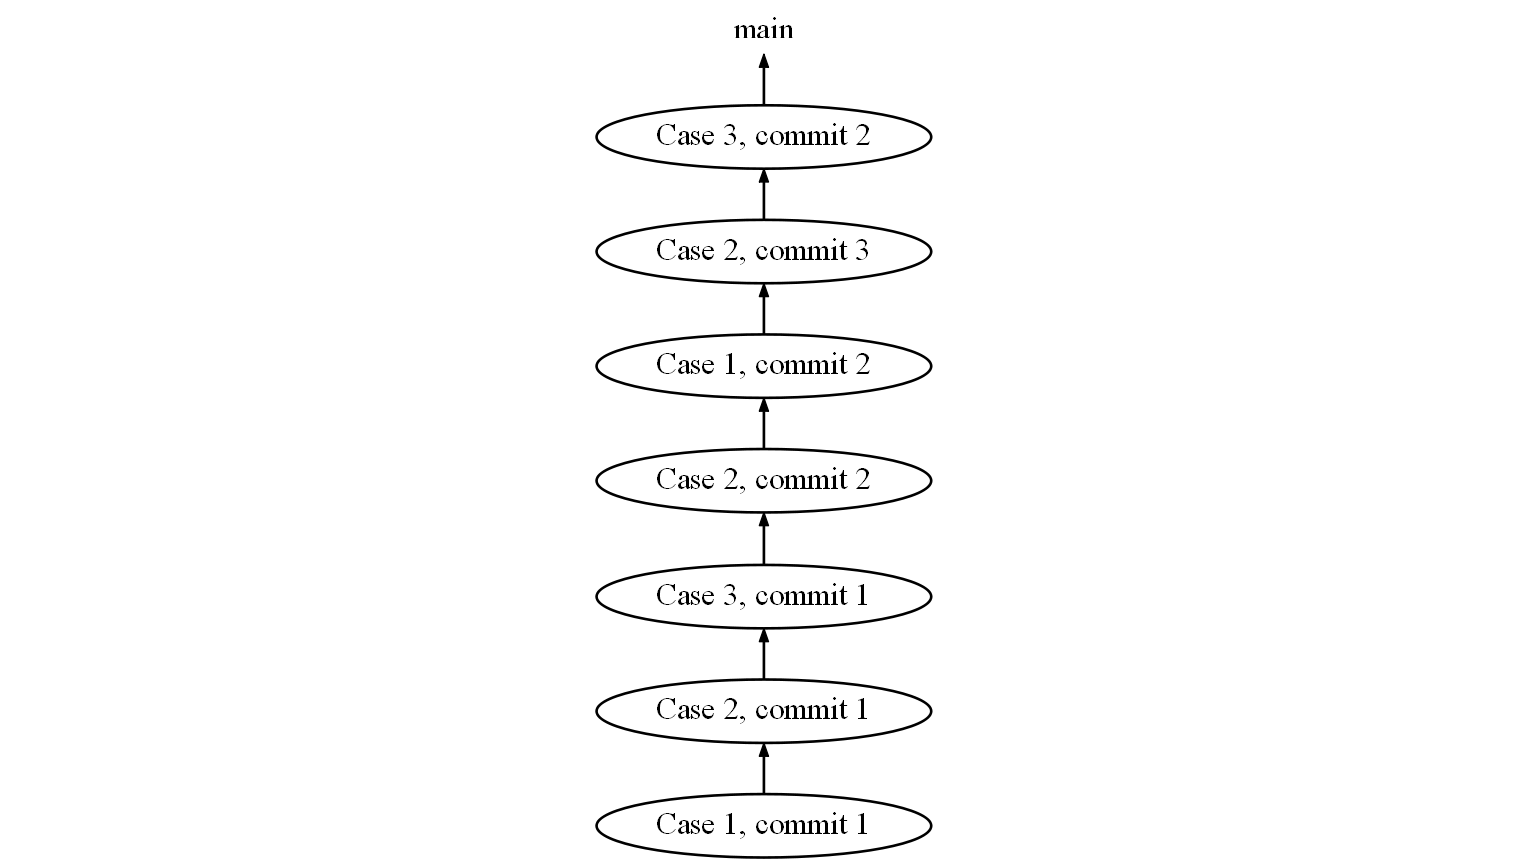
\includegraphics[scale=0.2]{02_2014_only-main.png}
\end{figure}

При ветвлении коммиты группируются по кейсам:
\begin{figure}[h!]
  \centering
  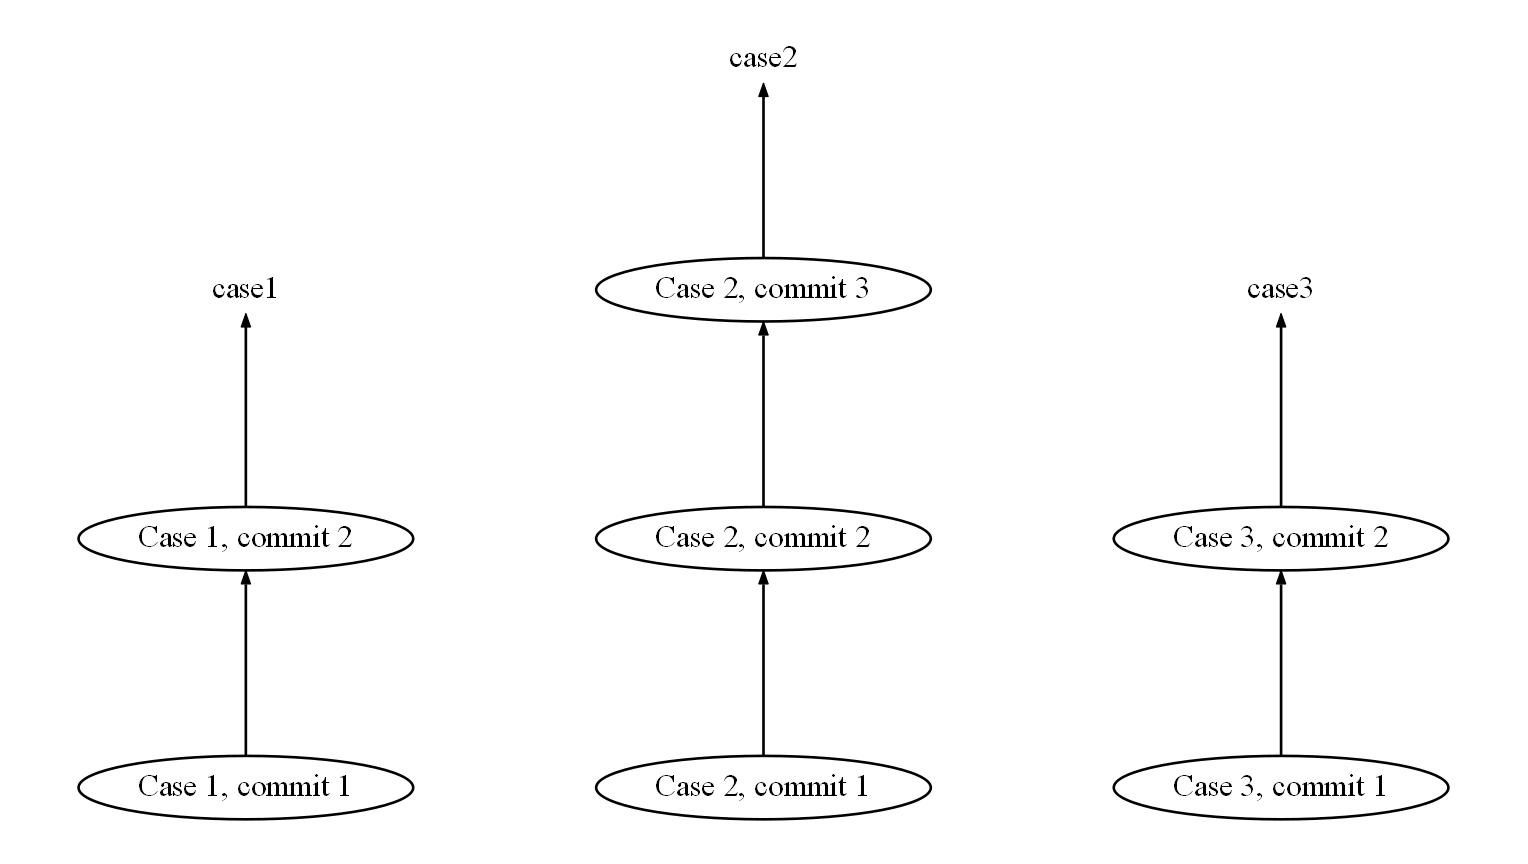
\includegraphics[scale=0.2]{02_2014_branches.png}
\end{figure}

\subsubsection*{Rebasing}

Rebasing может применяться в процессе работы над кейсом, а также для доставки коммитов в mainline.

Rebasing в процессе работы позволяет:

\begin{itemize}
  \item Получить ответвление от обновлённого mainline.
  \item Разрешать merge-conflicts небольшими порциями в ходе работы, а не одним большим куском в самом конце.
  \item Тестировать код своего кейса относительно нового mainline без его доставки в этот самый mainline.
\end{itemize}

Rebase вместо Merge как метод доставки кода в mainline позволяет получить:

\begin{itemize}
  \item Линейную историю в VCS. Линия проще и наглядней графа.
  \item Меньше проблем с blame, bisect и revert. Эти команды работают лучше на коммитах с одним родителем, чем с несколькими.
  \item Возможность удалять очень старые ветки (и их коммиты) из репозитория. Это повышает быстродействие репозитория. А если эти ветки всё-таки нужны "--- их можно хранить в архивном репозитории или в бэкапе. Тем, кто считает замедление репозитория при увеличении количества коммитов надуманной проблемой, есть смысл ознакомиться с исследованием Facebook \cite{Hlebnikov1}.
\end{itemize}

При доставке кода в mainline через Merge, mainline состоит в основном из merge-коммитов:
\begin{figure}[h!]
  \centering
  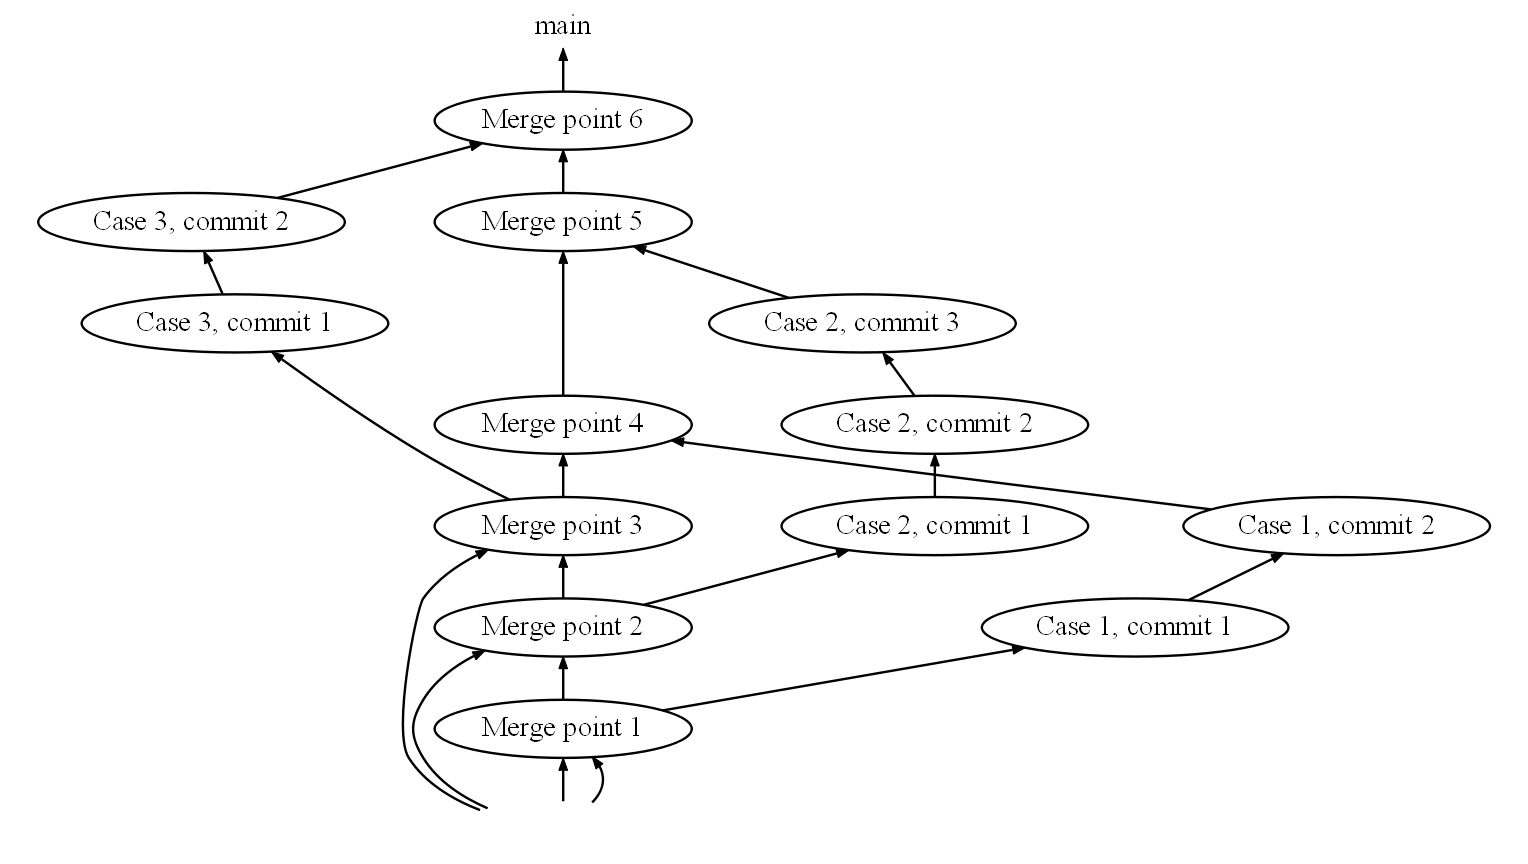
\includegraphics[scale=0.2]{02_2014_main-merged.png}
\end{figure}

Тот же самый граф, но без ярко выраженного вертикального mainline:
\begin{figure}[h!]
  \centering
  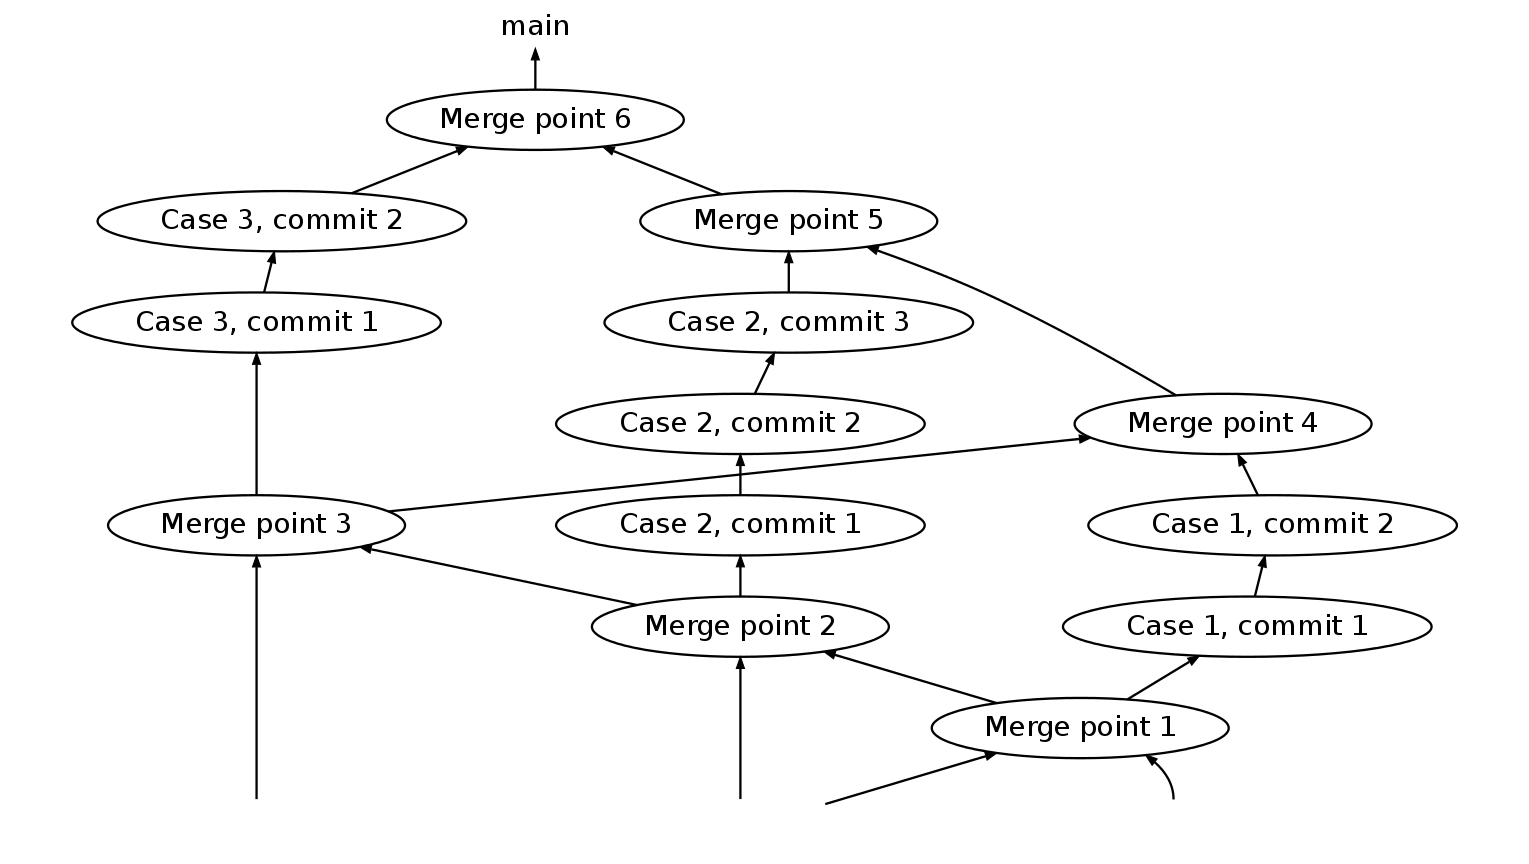
\includegraphics[scale=0.2]{02_2014_main-merged-weak-mainline.png}
\end{figure}

Как видно, в такой истории довольно трудно разобраться, особенно по прошествии долгого времени, или если разбирающийся "--- новый человек на проекте. В этом графе даже mainline трудно найти.

А вот история, которая получается при Rebase:
\begin{figure}[h!]
  \centering
  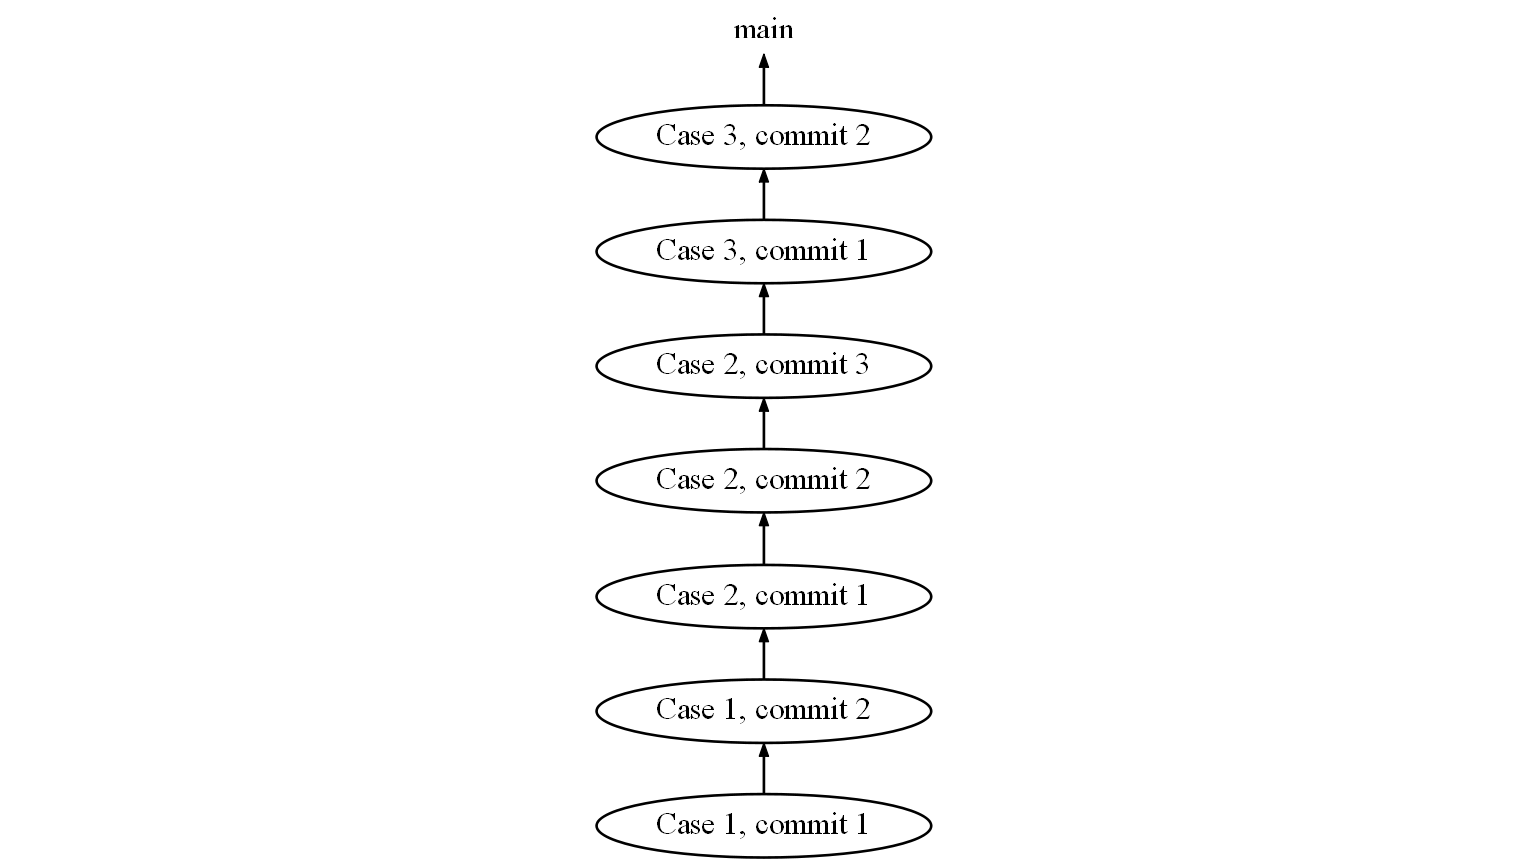
\includegraphics[scale=0.2]{02_2014_main-ordered.png}
\end{figure}

Как видно, история линейна, что сильно улучшает её читаемость. Но можно сделать ещё лучше "--- уменьшить количество коммитов. И в этом поможет squashing.

\subsubsection*{Squashing}

Squashing "--- это слияние нескольких коммитов в один. Squashing позволяет получить:

\begin{itemize}
  \item Компактную историю. Это тем важнее, чем дольше идёт разработка и чем больше коммитов собралось в репозитории.
  \item Меньше мусора в истории.
  \item Более лёгкий откат изменений.
\end{itemize}

Если после работы над кейсом ветка содержит много мусора в истории\ldots{}
\begin{figure}[h!]
  \centering
  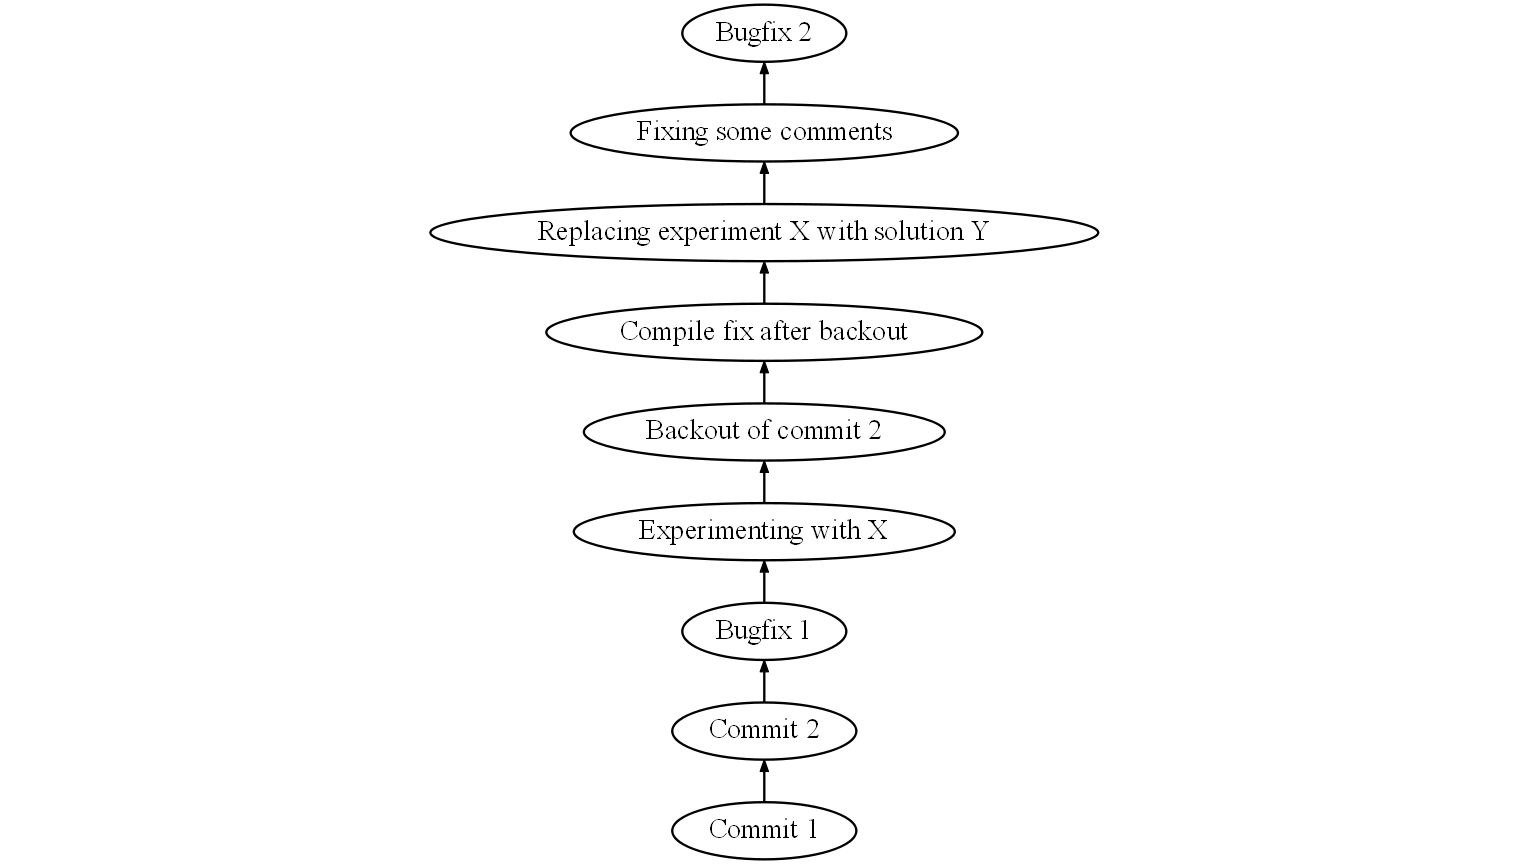
\includegraphics[scale=0.2]{02_2014_history-with-garbage.png}
\end{figure}

\ldots{}squashing позволит избавиться от этого мусора, слив все комиты в один:
\begin{figure}[h!]
  \centering
  
\includegraphics[scale=0.3]{02_2014_history-without-garbage.png}
\end{figure}

\subsection*{Конкретные команды, шаг за шагом}

Приведем примеры команд для Git и Mercurial в виде таблицы:

\begin{table}
  \centering
  \begin{tabular}{P{2.5cm}|P{3.5cm}|P{3.5cm}}
    \hline
                                  ~  & \textbf{Git}                   & \textbf{Mercurial}          \\ \hline
    Ответвление от mainline          & git checkout -{}-b case4       & hg book case4              \\
    Работа над кейсом                & git commit -m "Commit 1" \newline
                                       git commit -m "Commit 2" \ldots{}
                                                                    & hg commit -m "Commit 1" \newline
                                                                      hg commit -m "Commit 2" \ldots{} \\
    Rebase и squash              & git checkout -{}-b \emph{case4-2} \newline
                                   git rebase -{}-interactive main
                                                     & (нужны расширения rebase и histedit) \newline
                                                       hg rebase -{}-keep -{}-dest main \newline
                                                       hg histedit main \newline
                                                       hg book \emph{case4-2}      \\
    \hline
  \end{tabular}
\end{table}
Отдельно коснёмся «табу на rebase после push». Существует довольно распространённый миф, что если ветка запушена (push) на сервер "--- все возможности ребэйса (rebase) для неё потеряны, потому что если ветку проребэйсить и запушить на сервер опять (что возможно только с ключом --force), то это создаст несоответствие между репозиторием на сервере и репозиториями других разработчиков. В результате эти разработчики при попытке подтянуть эту ветку с сервера получат сломанную ветку.

На самом деле rebase возможен, если выполнять его правильно. На примере команд, приведённых в таблице, видно, что при ребэйсинге создаётся новая ветка, \textbf{case4-2}. Это принципиальный момент. Первоначальная ветка, \textbf{case4}, так и остаётся на своём месте, и получается аналог copy-on-write. Таким образом консистентность репозитория не нарушается, и ветка case4 не ломается "--- она просто устаревает. Теперь про неё можно забыть, а дальнейшую разработку, если она ещё продолжается, вести на ветке case4-2.

Также следует обратить внимание на ключ --interactive для Git и команду histedit для Mercurial. В результате их использования Git или Mercurial вызывают текстовый редактор, в котором разработчик может редактировать историю своей ветки: помечать коммиты для правки комментария, сливать несколько коммитов вместе, менять коммиты местами, удалять ненужные коммиты.

В сущности, многие коммиты "--- просто мусор в истории VCS: неудавшиеся эксперименты, багфиксы, фиксы компиляции, чистка неиспользуемых переменных, исправления опечаток в комментариях. Подобный материал в истории VCS не представляет ровным счётом никакого интереса. Как правило, от разработчика требуется имплементация фичи X или исправление бага Y, и желательно одним куском (то есть, как правило (хоть и не всегда), одним коммитом). А детали того, через что разработчик прошёл в процессе разработки, никого не интересуют. По этой причине мелкие правящие коммиты всегда имеет смысл объединить с «главными» коммитами, которые они дополняют. Это же относится и к фиксам в результате code review.

Делать слишком много «главных» коммитов для одного кейса тоже не имеет смысла. Наоборот, для большинства кейсов перед доставкой кода в mainline лучше слить все коммиты в один и использовать название кейса как комментарий этого единственного коммита. Если имел место рефакторинг без изменения функциональности "--- его имеет смысл выделить в отдельный коммит. Если имели место фиксы багов mainline'a, которые проявились при работе над данным кейсом "--- их тоже имеет смысл выделить в отдельные коммиты, и поместить эти коммиты перед основной разработкой. Других коммитов не нужно. Это и есть squashing "--- слияние нескольких коммитов в один.

Кроме чистки мусора в истории squashing также помогает убрать коммиты, которые не компилируются, путём слияния с фиксом компиляции. Это важно, если  используется bisect, а также в случае отката изменений.

Если вам захочется оставить в истории VCS свои чаяния и веяния по поводу данного кейса из ностальгических соображений "--- есть возможность сохранить их только для себя на той старой ветке case4, которая была любезно сохранена при copy-on-write-rebase. Не перетаскивая свой мусор в mainline, разработчик заодно не создает аналогичного искушения для товарищей по команде.

\subsection*{Доставка кода в mainline}

Итак, работа над кейсом завершена, код кейса оттестирован с новейшим mainline. После финальных rebase и squash на ветке должна находиться краткая и красивая история кейса, а сама ветка основана на верхушке mainline. Это и есть подходящий момент для доставки кода кейса в mainline. Для этого надо всего лишь переместить указатель mainline вперёд по ветке case4-2 "--- сделать fast-forward. Это можно сделать несколькими способами; автор предпочитает такие:

\begin{table}
  \centering
  \begin{tabular}{P{3.5cm}|P{6cm}} \hline
    \textbf{Git}                       & \textbf{Mercurial}            \\ \hline
     git push . case4-2:main      & (hg update case4-2) \linebreak
                               hg book main \linebreak  \# «book» does fast-forward \linebreak
                               \# in this case                                               \\ \hline
  \end{tabular}
\end{table}
Важно обратить внимание на точку после git push. Она означает «текущий репозиторий». Однако можно пушить и сразу в origin:

git push origin case4-2:main

При этом не следует опасаться поломки origin/main, т.к. если предлагаемый push не fast-forward, Git не позволит выполнить push без ключа -{}-force.

\subsection*{Выводы}

В результате использования предложенного подхода мы получаем:

\begin{itemize}
  \item Удобство разработки на отдельных ветвях.
  \item Возможность всегда работать и тестировать свои изменения относительно новейшего mainline.
  \item Линейную историю.
  \item Группировку коммитов по кейсам.
  \item Безупречную и компактную историю без мусора.
\end{itemize}

\begin{figure}[h!]
  \centering
  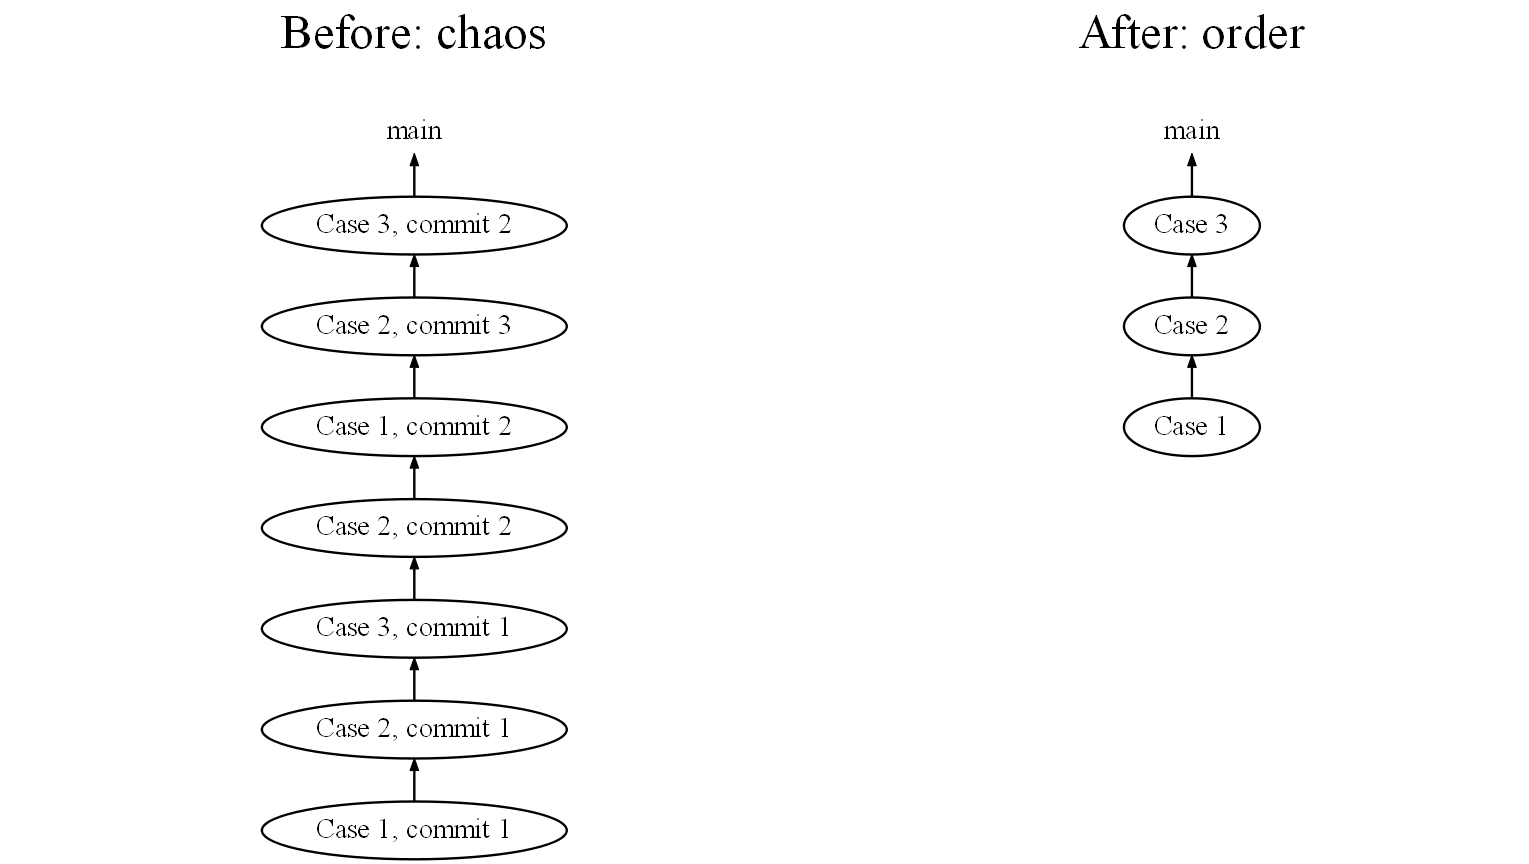
\includegraphics[scale=0.2]{02_2014_before-vs-after.png}
\end{figure}

\begin{thebibliography}{9}
\bibitem{Hlebnikov1} \url{http://thread.gmane.org/gmane.comp.version-control.git/189776}
\end{thebibliography}
\end{document}

\documentclass[10pt, a5paper]{article}
\usepackage{pdfpages}
\usepackage{parallel}
\usepackage[T2A]{fontenc}
\usepackage{ucs}
\usepackage[utf8x]{inputenc}
\usepackage[polish,english,russian]{babel}
\usepackage{hyperref}
\usepackage{rotating}
\usepackage[inner=2cm,top=1.8cm,outer=2cm,bottom=2.3cm,nohead]{geometry}
\usepackage{listings}
\usepackage{graphicx}
\usepackage{wrapfig}
\usepackage{longtable}
\usepackage{indentfirst}
\usepackage{array}
\newcolumntype{P}[1]{>{\raggedright\arraybackslash}p{#1}}
\frenchspacing
\usepackage{fixltx2e} %text sub- and superscripts
\usepackage{icomma} % коскі ў матэматычным рэжыме
\PreloadUnicodePage{4}

\newcommand{\longpage}{\enlargethispage{\baselineskip}}
\newcommand{\shortpage}{\enlargethispage{-\baselineskip}}

\def\switchlang#1{\expandafter\csname switchlang#1\endcsname}
\def\switchlangbe{
\let\saverefname=\refname%
\def\refname{Літаратура}%
\def\figurename{Іл.}%
}
\def\switchlangen{
\let\saverefname=\refname%
\def\refname{References}%
\def\figurename{Fig.}%
}
\def\switchlangru{
\let\saverefname=\refname%
\let\savefigurename=\figurename%
\def\refname{Литература}%
\def\figurename{Рис.}%
}

\hyphenation{admi-ni-stra-tive}
\hyphenation{ex-pe-ri-ence}
\hyphenation{fle-xi-bi-li-ty}
\hyphenation{Py-thon}
\hyphenation{ma-the-ma-ti-cal}
\hyphenation{re-ported}
\hyphenation{imp-le-menta-tions}
\hyphenation{pro-vides}
\hyphenation{en-gi-neering}
\hyphenation{com-pa-ti-bi-li-ty}
\hyphenation{im-pos-sible}
\hyphenation{desk-top}
\hyphenation{elec-tro-nic}
\hyphenation{com-pa-ny}
\hyphenation{de-ve-lop-ment}
\hyphenation{de-ve-loping}
\hyphenation{de-ve-lop}
\hyphenation{da-ta-ba-se}
\hyphenation{plat-forms}
\hyphenation{or-ga-ni-za-tion}
\hyphenation{pro-gramming}
\hyphenation{in-stru-ments}
\hyphenation{Li-nux}
\hyphenation{sour-ce}
\hyphenation{en-vi-ron-ment}
\hyphenation{Te-le-pathy}
\hyphenation{Li-nux-ov-ka}
\hyphenation{Open-BSD}
\hyphenation{Free-BSD}
\hyphenation{men-ti-on-ed}
\hyphenation{app-li-ca-tion}

\def\progref!#1!{\texttt{#1}}
\renewcommand{\arraystretch}{2} %Іначай формулы ў матрыцы зліпаюцца з лініямі
\usepackage{array}

\def\interview #1 (#2), #3, #4, #5\par{

\section[#1, #3, #4]{#1 -- #3, #4}
\def\qname{LVEE}
\def\aname{#1}
\def\q ##1\par{{\noindent \bf \qname: ##1 }\par}
\def\a{{\noindent \bf \aname: } \def\qname{L}\def\aname{#2}}
}

\def\interview* #1 (#2), #3, #4, #5\par{

\section*{#1\\{\small\rm #3, #4. #5}}

\def\qname{LVEE}
\def\aname{#1}
\def\q ##1\par{{\noindent \bf \qname: ##1 }\par}
\def\a{{\noindent \bf \aname: } \def\qname{L}\def\aname{#2}}
}

\begin{document}
\title{Коммерциализаия СПО под GPL лицензией}
\author{Александр Рябиков, Сергей Середа "--- Москва, РФ\footnote{\url{rsashka@mail.ru}, \url{http://lvee.org/en/abstracts/121}}}
\maketitle
\begin{abstract}
In accordance to main goals of ADempiere Foundation our task was to find a way to get return on investments in Free Software modification/enhancement for a SMB developer company without dual licensing and without accompanying the product with proprietary add"=ons/plugins or additional services or merchandise. Also there were a need to provide a mechanism of costs' sharing between several interested SMB companies.

After initial economic analysis we've concluded that the only way to get return on investments in free software development is to create a time lag between the moment of software product provision to a user and the moment of rights provision for this software according to GPL. Otherwise, demand and supply law just will not work with free software.

Also we have studied the legislation and FSF Comprehensive FAQ about the GNU Licenses. As a result, there were constructed two schemes that could create such time lag without GPL violation. 

First is based mostly on GNU FAQ, second is based on the provisions of contract law.
\end{abstract}
%\begin{center}\textbf{Фонд поддержки и развития делового свободного программного обеспечения ``Адемпиере''}\end{center}

%\begin{flushright}Авторы: 
%Александр Рябиков, 
%Сергей Середа, к.э.н.,\end{flushright}

\subsection*{СПО под GPL лицензией}

Как известно, “свободные” лицензии дают конечным пользователям полную свободу, в том числе и свободу распространять конечный программный продукт наравне с разработчиком. А это означает, что каждый раз, когда разработчик продаёт копию ПО под “свободной” лицензией, он создает себе конкурента. Принято считать, что невозможно зарабатывать деньги непосредственно на доработке и распространении свободного программного обеспечения, распространяемого на условиях GPL или совместимых с нею лицензий. Описываемые в литературе и применяемые на практике бизнес"=модели практически безусловно предполагают бесплатное (или за символическую плату) распространение таких программ. В противоположность этому, наличие “традиционной” (на жаргоне называемой “проприетарной”) лицензии позволяет зарабатывать непосредственно на распространении программного обеспечения.

Обладателю исключительных прав на программу ещё доступна модель двойного лицензирования, подразумевающая “несвободную” коммерческую лицензию на ПО для бизнес"=заказчиков и GPL"=совместимую лицензию  для представителей сообщества. Для всех же вторичных проектов (так называемых “форков”) подобная возможность исключена. Любые доработки кода для ПО, выпущенного под GPL, могут быть выпущены только под этой же или совместимой “вирусной” лицензией, а замена GPL на несовместимую лицензию допускается только с согласия всех обладателей исключительных прав на программу.

С учетом этого, считается, что зарабатывать на Free Software, не являясь обладателем прав на оригинальный продукт, можно либо оказывая сервисные услуги (сопровождение, документирование, обучение и т.п.), либо компонуя его с собственными разработками с закрытым исходным кодом, способом, который допускается используемой свободной лицензией.

Описываемый ниже способ коммерциализации доработок свободного ПО позволит в определенной мере изменить сложившуюся ситуацию. Предлагаемая бизнес"=модель предназначена, в основном для b2b"=разработчиков, развивающих уже существующие свободные программные продукты, но не владеющих исключительным правом на сам продукт (т.е. наиболее часто встречающаяся ситуация).

Суть бизнес"=модели сводится к созданию условий, аналогичных “традиционному” модели распространения программного обеспечения, т.е. к “продаже” доработанного продукта сразу нескольким покупателям, что даст возможность окупить понесенные затраты на доработку СПО за счет их многократной продажи. Такой эффект достигается за счет создания временного лага между началом продаж доработанного программного продукта и моментом его размещения в свободном доступе для бесплатной загрузки, что позволяет разработчику стать, на какое"=то время, единственным продавцом, у кого эти доработки можно будет приобрести.

Особенность предлагаемой модели заключается в том, что при этом не происходит ни изменения, ни нарушения условий “вирусного” лицензионного соглашения "--- эффективное ограничение распространения продукта определяется договором между хозяйствующими субъектами и вытекает из процесса выполнения заказных программных разработок.

\subsection*{1. Решение, «подсказанное» Free Software \linebreak Foundation (FSF)}

Временной лаг создаётся за счёт превращения пользователя в (со)разработчика, подписания с ним соглашения о нераспространении экземпляров продукта и предоставления ему программного обеспечения для тестирования на продуктивных данных.

\subsubsection*{Часто забываемые факты о GPL}

\begin{itemize}
  \item GPL допускает платное распространение программ \cite{ryabikov1}.
  \item GPL не требует от разработчика делать исходные коды своих разработок доступными широкой публике \cite{ryabikov2}.
  \item Разработчик не вправе запрещать Заказчику дальнейшее распространение ПО \cite{ryabikov3, ryabikov4}.
  \item GPL позволяет Заказчику запретить разработчику распространять результаты заказной разработки  \cite{ryabikov5}.
\end{itemize}

\subsection*{Сценарий по «подсказке» FSF}

Исходная ситуация: Разработчиком доработан GPL"=продукт, \linebreak есть компания"=пользователь, желающая внедрить доработанный \linebreak продукт, но не готовая оплатить полную стоимость доработки, Разработчику необходимо обеспечить возврат инвестиций в доработку, но есть риск, что компания"=пользователь опубликует доработки, как только получит к ним доступ.

\subsubsection*{Предлагаемая схема взаимодействия к компанией"=пользователем:}

\begin{itemize}
  \item Разработчик продает компании"=пользователю исходный продукт без своих доработок.
  \item Разработчик нанимает компанию"=пользователя для выполнения работ, связанных с новым кодом, в частности, для тестирования.
  \item В соответствии с комментариями FSF \cite{ryabikov5} существует законная возможность ограничить распространение тестируемого кода на время действия соответствующего договора.
  \item Время действия этого договора и будет определять временной лаг между началом распространения доработок GPL продукта и моментом его появления в свободном доступе.
  \item Разработчик может одновременно работать по такой схеме сразу с несколькими заинтересованными компаниями.
\end{itemize}

\subsection*{2. Решение на основе договорного права}

Временной лаг создаётся за счёт того, что права на созданный по заказу код и возможность его дальнейшего распространения возникают только после полного исполнения обязательств сторонами договора на доработку ПО.

\subsubsection*{Сценарий на основе договорного права}

Исходная ситуация: Разработчиком доработан GPL"=продукт \linebreak  (разработчик готов его доработать), есть компания"=пользователь, желающая внедрить доработанный продукт, но не готовая оплатить полную стоимость доработки, Разработчику необходимо обеспечить возврат инвестиций в доработку, но есть риск, что компания"=пользователь опубликует доработки, как только получит к ним доступ.

\subsubsection*{Предлагаемая схема взаимодействия к компанией"=пользователем:}

\begin{itemize}
  \item Разработчик заключает с компанией"=пользователем договор на доработку исходного GPL продукта.
  \item В соответствии с действующим законодательством РФ (Статья 712. Право подрядчика на удержание, Статья 1296. Программы для ЭВМ и базы данных, созданные по заказу), в этом случае существует законная возможность ограничить распространение тестируемого кода на время действия соответствующего договора.
  \item Время действия этого договора и будет определять временной лаг между началом распространения доработок продукта под GPL лицензией и моментом его появления в свободном доступе.
  \item Разработчик может одновременно работать по такой схеме сразу с несколькими заинтересованными компаниями.
\end{itemize}

Описанная конструкция не является каким"=то искусственным построением. Наоборот, она является описанием вполне реального процесса заказной разработки корпоративного ПО, который завершается только после проведения опытной или опытно"=промышленной эксплуатации разработок (с их полным сопровождением все это время) и передачи их в промышленную эксплуатацию.

По мнению авторов, регулируя длительность временного лага между началом продаж доработанного программного продукта и моментом его размещения в свободном доступе для бесплатной загрузки, в зависимости от типа, сложности, популярности и иных характеристик дорабатываемого программного продукта, можно обеспечить возврат инвестиций в его развитие, достаточный для поддержания коммерческого предприятия. При этом, за счет заключения подобных договоров с несколькими (в идеале "--- со многими) пользователями"=заказчиками будет также обеспечено и разделение затрат между ними (в отличие от схемы bounty source, в рамках которой доработка целиком оплачивается одним заказчиком).

Конечно, наложение любых ограничений на распространение СПО может быть воспринято “в штыки” сообществом и, возможно, потребуются определенные усилия, что бы сторонники двух диаметрально противоположных точек зрения на способы распространения ПО смогли оценить положительные и отрицательные стороны от такого “нововведения”. Тем не менее, описанная бизнес"=модель полностью основана на законе и не нарушает ни одного положения о защите интеллектуальной собственности. Более того, она, по сути, является просто специализированной модификацией широко применяемой в корпоративном секторе стандартной модели заказной разработки ПО.

Мы обсудили с Ричардом Столлманом эти способы и он сделал важные замечания к описываемым моделям. Второй способ на основе контрактного права соответствует GPLv2, но нарушает GPLv3, где в явном виде прописано, что лицензия имеет приоритет над контрактными обязательствами. С этим мнением не согласны наши юристы, но кто из них прав может решить только судебная практика.
Насчет первого способа, Ричард конечно не в восторге, но нарушение GPL будет в том случае, если работа пользователя будет фиктивной. Другими словами, пользователь должен по настоящему работать в соответствии с контрактными обязательствами и эта работа должна реально оплачиваться.

Конечно, используя описанные выше принципы, первое время код будет отсутствовать в свободном доступе, но через какое то время он все равно станет доступен для всех. И в результате, и инвесторы вернут вложенные средства и сообщество получит ощутимый вклад в развитие СПО.

Данная методика коммерциализации СПО с лицензией GPL была представлена на Russian Open Source Summit 2014. Статья по материалам доклада доступна на сайте PCWEEK \cite{ryabikov6}.

\begin{thebibliography}{9}
\bibitem{ryabikov1} \url{http://www.gnu.org/licenses/gpl-faq.en.html#DoesTheGPLAllowMoney}
\bibitem{ryabikov2} \url{http://www.gnu.org/licenses/gpl-faq.en.html#DoesTheGPLRequireAvailabilityToPublic}
\bibitem{ryabikov3} \url{http://www.gnu.org/licenses/gpl-faq.en.html#DoesTheGPLAllowNDA}
\bibitem{ryabikov4} \url{http://www.gnu.org/licenses/gpl-faq.en.html#DoesTheGPLAllowModNDA}
\bibitem{ryabikov5} \url{http://www.gnu.org/licenses/gpl-faq.en.html#DevelopChangesUnderNDA}
\bibitem{ryabikov6} \url{http://www.pcweek.ru/foss/article/detail.php?ID=164583}
\end{thebibliography}
\end{document}

\documentclass[10pt, a5paper]{article}
\usepackage{pdfpages}
\usepackage{parallel}
\usepackage[T2A]{fontenc}
\usepackage{ucs}
\usepackage[utf8x]{inputenc}
\usepackage[polish,english,russian]{babel}
\usepackage{hyperref}
\usepackage{rotating}
\usepackage[inner=2cm,top=1.8cm,outer=2cm,bottom=2.3cm,nohead]{geometry}
\usepackage{listings}
\usepackage{graphicx}
\usepackage{wrapfig}
\usepackage{longtable}
\usepackage{indentfirst}
\usepackage{array}
\newcolumntype{P}[1]{>{\raggedright\arraybackslash}p{#1}}
\frenchspacing
\usepackage{fixltx2e} %text sub- and superscripts
\usepackage{icomma} % коскі ў матэматычным рэжыме
\PreloadUnicodePage{4}

\newcommand{\longpage}{\enlargethispage{\baselineskip}}
\newcommand{\shortpage}{\enlargethispage{-\baselineskip}}

\def\switchlang#1{\expandafter\csname switchlang#1\endcsname}
\def\switchlangbe{
\let\saverefname=\refname%
\def\refname{Літаратура}%
\def\figurename{Іл.}%
}
\def\switchlangen{
\let\saverefname=\refname%
\def\refname{References}%
\def\figurename{Fig.}%
}
\def\switchlangru{
\let\saverefname=\refname%
\let\savefigurename=\figurename%
\def\refname{Литература}%
\def\figurename{Рис.}%
}

\hyphenation{admi-ni-stra-tive}
\hyphenation{ex-pe-ri-ence}
\hyphenation{fle-xi-bi-li-ty}
\hyphenation{Py-thon}
\hyphenation{ma-the-ma-ti-cal}
\hyphenation{re-ported}
\hyphenation{imp-le-menta-tions}
\hyphenation{pro-vides}
\hyphenation{en-gi-neering}
\hyphenation{com-pa-ti-bi-li-ty}
\hyphenation{im-pos-sible}
\hyphenation{desk-top}
\hyphenation{elec-tro-nic}
\hyphenation{com-pa-ny}
\hyphenation{de-ve-lop-ment}
\hyphenation{de-ve-loping}
\hyphenation{de-ve-lop}
\hyphenation{da-ta-ba-se}
\hyphenation{plat-forms}
\hyphenation{or-ga-ni-za-tion}
\hyphenation{pro-gramming}
\hyphenation{in-stru-ments}
\hyphenation{Li-nux}
\hyphenation{sour-ce}
\hyphenation{en-vi-ron-ment}
\hyphenation{Te-le-pathy}
\hyphenation{Li-nux-ov-ka}
\hyphenation{Open-BSD}
\hyphenation{Free-BSD}
\hyphenation{men-ti-on-ed}
\hyphenation{app-li-ca-tion}

\def\progref!#1!{\texttt{#1}}
\renewcommand{\arraystretch}{2} %Іначай формулы ў матрыцы зліпаюцца з лініямі
\usepackage{array}

\def\interview #1 (#2), #3, #4, #5\par{

\section[#1, #3, #4]{#1 -- #3, #4}
\def\qname{LVEE}
\def\aname{#1}
\def\q ##1\par{{\noindent \bf \qname: ##1 }\par}
\def\a{{\noindent \bf \aname: } \def\qname{L}\def\aname{#2}}
}

\def\interview* #1 (#2), #3, #4, #5\par{

\section*{#1\\{\small\rm #3, #4. #5}}

\def\qname{LVEE}
\def\aname{#1}
\def\q ##1\par{{\noindent \bf \qname: ##1 }\par}
\def\a{{\noindent \bf \aname: } \def\qname{L}\def\aname{#2}}
}

\begin{document}
\title{Text parsing with python and PLY}
\author{Даниил Батурин "--- Томск, РФ\footnote{\url{daniil@baturin.org}, \url{http://lvee.org/en/abstracts/122}}}
\maketitle
\begin{abstract}
Language parsing is a common software development problem. Python is widely used in both production software development and rapid prototyping, and a number of lexer and parser generators were written for it.
In this talk we discuss using one of them, PLY, which is a pure python implementation of classic lex and YACC tools, for parsing a made-up configuration file grammar.
\end{abstract}
Formal language parsing is a common problem in software development. Standardized formats with already available parsing libraries, such as XML and JSON, have simplified the problem, but did not completely remove it. Python is widely used as a general purpose programming language as well as one for rapid prototyping, so Python programmers face this task as well.

There is a number of parser generators for Python, which use different algorithms and APIs. In this talk we discuss PLY that is a pure Python implementation of classic UNIX tools: lex scanner generator, and YACC parser generator. It is maintained by David Beazley and distributed under thee-clause BSD license.

Lex and YACC are there for decades and have been reimplemented not once. This makes PLY easy to learn for UNIX programmers and relatively easy to convert the Python code into C/C++ if needed.

\subsection*{Parsing basics}

There are three typical approaches to make a parser:

\begin{enumerate}
  \item write an ad hoc parser manually,
  \item use a parser generator,
  \item write an advanced parsing algorithm manually.
\end{enumerate}

Ad hoc parsers are suitable for simple grammars, but tend to quickly become hard to maintain and modify. Coding an advanced parsing algorithm like an LL parser is usually redundant and only feasible for very complex grammars or in case of special requirements. For the majority of grammars a parser produced with some parser generator is usually the best option.

Most parser implementations do not work directly with the character stream but use a \emph{token} stream produced by a \emph{scanner}. Using a separate scanner (also known as lexer) to break the stream into tokens simplifies the task as it allows to write grammar rules in terms of token names rather than literal strings, e.g. all arithmetic operators can be referred to as OPSIGN token in a rule for arithmetic expressions. Scanner code is usually generated automatically from a set of regular expressions as well.

The most common algorithm used by parser generators is LALR (1) that reads tokens until a sequence matching the entire grammar rule is found.

\subsection*{Using PLY}

PLY consists of two modules, \verb!ply.lex! and \verb!ply.yacc!. Actions for tokens and grammar rules are defined as functions, while token regular expressions and grammar rules are defined in function docstrings. Tokens that need no actions can be defined as variables.

A simple parser for breaking into parts a line consisting of letters and digits groups separated by semicolon will look like:

\begin{verbatim}
import re
import ply.lex as lex
import ply.yacc as yacc

## Lexer part
tokens = ( 'LETTER', 'DIGIT', 'SEMI' )

t_LETTER = r'[a-z]'

def t_DIGIT(t):
    r'[0-9]'
    t.value = int(t.value)
    return t

t_SEMI = r';'
t_ignore = r' '

lexer = lex.lex(debug=1)

## Parser part
start = 'start'

def p_letter_digit_pair(p):
    ''' pair : LETTER DIGIT SEMI '''
    p[0] = (p[1], p[2])

def p_pair_group(p):
    ''' pair_group : pair_group pair
                   | pair
    '''
    print p[0], p[1]
    p[0] = [p[1]] if len(p) == 2 else p[1] + [p[2]]

start = 'pair_group'

parser = yacc.yacc(debug=1)

## Test it
s = "a 0; b 1; c 2;"
print(parser.parse(s))
\end{verbatim}

A more elaborate example discussed in the conference talk can be found at \url{https://github.com/dmbaturin/ply-example}


\begin{thebibliography}{9}
\bibitem{baturin1} PLY website. \url{http://www.dabeaz.com/ply/}
\bibitem{baturin2} Pete Jinks, The Implementation and Power of Programming Languages. \url{http://www.cs.man.ac.uk/~pjj/cs212/ho/ho.html}
\end{thebibliography}

\end{document}

\documentclass[10pt, a5paper]{article}
\usepackage{pdfpages}
\usepackage{parallel}
\usepackage[T2A]{fontenc}
\usepackage{ucs}
\usepackage[utf8x]{inputenc}
\usepackage[polish,english,russian]{babel}
\usepackage{hyperref}
\usepackage{rotating}
\usepackage[inner=2cm,top=1.8cm,outer=2cm,bottom=2.3cm,nohead]{geometry}
\usepackage{listings}
\usepackage{graphicx}
\usepackage{wrapfig}
\usepackage{longtable}
\usepackage{indentfirst}
\usepackage{array}
\newcolumntype{P}[1]{>{\raggedright\arraybackslash}p{#1}}
\frenchspacing
\usepackage{fixltx2e} %text sub- and superscripts
\usepackage{icomma} % коскі ў матэматычным рэжыме
\PreloadUnicodePage{4}

\newcommand{\longpage}{\enlargethispage{\baselineskip}}
\newcommand{\shortpage}{\enlargethispage{-\baselineskip}}

\def\switchlang#1{\expandafter\csname switchlang#1\endcsname}
\def\switchlangbe{
\let\saverefname=\refname%
\def\refname{Літаратура}%
\def\figurename{Іл.}%
}
\def\switchlangen{
\let\saverefname=\refname%
\def\refname{References}%
\def\figurename{Fig.}%
}
\def\switchlangru{
\let\saverefname=\refname%
\let\savefigurename=\figurename%
\def\refname{Литература}%
\def\figurename{Рис.}%
}

\hyphenation{admi-ni-stra-tive}
\hyphenation{ex-pe-ri-ence}
\hyphenation{fle-xi-bi-li-ty}
\hyphenation{Py-thon}
\hyphenation{ma-the-ma-ti-cal}
\hyphenation{re-ported}
\hyphenation{imp-le-menta-tions}
\hyphenation{pro-vides}
\hyphenation{en-gi-neering}
\hyphenation{com-pa-ti-bi-li-ty}
\hyphenation{im-pos-sible}
\hyphenation{desk-top}
\hyphenation{elec-tro-nic}
\hyphenation{com-pa-ny}
\hyphenation{de-ve-lop-ment}
\hyphenation{de-ve-loping}
\hyphenation{de-ve-lop}
\hyphenation{da-ta-ba-se}
\hyphenation{plat-forms}
\hyphenation{or-ga-ni-za-tion}
\hyphenation{pro-gramming}
\hyphenation{in-stru-ments}
\hyphenation{Li-nux}
\hyphenation{sour-ce}
\hyphenation{en-vi-ron-ment}
\hyphenation{Te-le-pathy}
\hyphenation{Li-nux-ov-ka}
\hyphenation{Open-BSD}
\hyphenation{Free-BSD}
\hyphenation{men-ti-on-ed}
\hyphenation{app-li-ca-tion}

\def\progref!#1!{\texttt{#1}}
\renewcommand{\arraystretch}{2} %Іначай формулы ў матрыцы зліпаюцца з лініямі
\usepackage{array}

\def\interview #1 (#2), #3, #4, #5\par{

\section[#1, #3, #4]{#1 -- #3, #4}
\def\qname{LVEE}
\def\aname{#1}
\def\q ##1\par{{\noindent \bf \qname: ##1 }\par}
\def\a{{\noindent \bf \aname: } \def\qname{L}\def\aname{#2}}
}

\def\interview* #1 (#2), #3, #4, #5\par{

\section*{#1\\{\small\rm #3, #4. #5}}

\def\qname{LVEE}
\def\aname{#1}
\def\q ##1\par{{\noindent \bf \qname: ##1 }\par}
\def\a{{\noindent \bf \aname: } \def\qname{L}\def\aname{#2}}
}

\begin{document}
\title{Bootloader and Linux kernel debugging on ARM board with OpenOCD}
\author{Vladimir Zapolskiy "--- Espoo, Finland\footnote{\url{vz@mleia.com}, \url{http://lvee.org/en/abstracts/126}}}
\maketitle
\begin{abstract}
The system software development in area of embedded systems is complicated by proximity to the physical world, incomplete knowledge of hardware errors and sophisticated existing software. Fortunately it is possible to reuse advantages of a debugger in development of operating systems and bootloaders with the aid of a bridge from hardware and running system software to the GDB session on a developer's workstation, which is provided by JTAG interface, a cheap JTAG-USB adapter and connective software from open source OpenOCD project.
\end{abstract}
Consider a task of a new device development from system programmer's point of view, and to immerse in the details let the device has any purpose but it complies with the following requirements:

\begin{itemize}
  \item the device is powered by ARMv4 or higher application processor, possibly multicore one,
  \item the ARM application processor executes bootloader, hypervisor or operating system kernel, and the developer has access to its source code, for instance U-boot bootloader and Linux kernel.
\end{itemize}

A system programmer of ARM powered embedded systems unavoidably meets a number of tasks and problems during the low-level development stage:

\begin{itemize}
  \item port a bootloader or Linux kernel to a new ARM SoC,
  \item port a bootloader or Linux kernel to a new device governed by some ARM SoC,
  \item add new features of arbitrary nature into a bootloader or Linux kernel,
  \item fix a bug in a bootloader or Linux kernel code,
  \item thoroughly perceive the work of a subcomponent in a bootloader or Linux kernel during runtime.
\end{itemize}

Arguably not all aforementioned tasks are related to debugging, but for simplicity let's call them debugging tasks, and let's find a handy debugger, which helps to resolve the problems listed above. One well-known by developers, favourable and powerful debugger is GNU Debugger or GDB \cite{Zapolskiy1}, and fortunately there is a way to utilize the same debugger for the introduced new challenges in the domain of low-level system programming, so GDB helps to debug not only applications, but bootloaders and operating systems.

One of the most popular methods of system code debugging is the control of application processor cores in runtime by means of boundary scan checking of integrated circuits according to JTAG specification (IEEE Std. 1149.1)\cite{Zapolskiy2}, and the considered ARM SoCs and most of development PCBs have such interface. There are commercial brand JTAG adapters from Lauterbach and Abatron, but due to many benefits (convenience and flexibility in use, price, advantages of open source software etc.) it is reasonable to use simple cheap JTAG-USB adaptors and the attendant supplementary managing code from the open source, constantly developing Open On-Chip Debugger project or OpenOCD\cite{Zapolskiy3}.

Functionally OpenOCD software paired with e.g. FT2232 powered JTAG-USB adapter successfully compete with notably more expensive brand alternatives. OpenOCD allows to write sophisticated Tcl scripts operating with the target CPU and board (for example, automated firmware upload, writing to a flash drive on board reset, etc.), scripts handling and post-processing events from cores, reading and modifying board RAM content and core registers, setting execution breakpoints and data read/write watchpoints, and also OpenOCD presents two user interaction interfaces, among which one is for low-level and manual operations via telnet protocol and another one serves as a GDB server. The latter familiar GDB server interface is conveniently utilized by a developer, who applies her/his ready practical knowledge of debugging with GDB and uses GDB open documentation, as well as add-ons -- for example, user's own GDB scripts or GDB frontends and IDEs like DDD, Emacs or Eclipse.

One of the powerful functions of GDB server from OpenOCD is the ability to debug in runtime the code execution on multiple CPU cores simultaneously by means of a GDB protocol extension. From the user's point of view it looks similarly to debugging a multithread application, but the role of an application is performed here by e.g. the Linux kernel.

For embedded software developers OpenOCD facilitates essentially the execution of any tasks mentioned in the beginning, and debugging a complex source code beneath the application level becomes easy and comprehensible, making OpenOCD a helpful tool and adding it to the system developer's must-have toolbox.


\begin{thebibliography}{9}
\bibitem{Zapolskiy1} The GNU Project Debugger, \url{https://www.gnu.org/software/gdb/}
\bibitem{Zapolskiy2} IEEE 1149.1-2013, \url{http://standards.ieee.org/findstds/standard/1149.1-2013.html}
\bibitem{Zapolskiy3} Open On-Chip Debugger, \url{http://openocd.sourceforge.net/doc/html/index.html}
\end{thebibliography}
\end{document}

\documentclass[10pt, a5paper]{article}
\usepackage{pdfpages}
\usepackage{parallel}
\usepackage[T2A]{fontenc}
\usepackage{ucs}
\usepackage[utf8x]{inputenc}
\usepackage[polish,english,russian]{babel}
\usepackage{hyperref}
\usepackage{rotating}
\usepackage[inner=2cm,top=1.8cm,outer=2cm,bottom=2.3cm,nohead]{geometry}
\usepackage{listings}
\usepackage{graphicx}
\usepackage{wrapfig}
\usepackage{longtable}
\usepackage{indentfirst}
\usepackage{array}
\newcolumntype{P}[1]{>{\raggedright\arraybackslash}p{#1}}
\frenchspacing
\usepackage{fixltx2e} %text sub- and superscripts
\usepackage{icomma} % коскі ў матэматычным рэжыме
\PreloadUnicodePage{4}

\newcommand{\longpage}{\enlargethispage{\baselineskip}}
\newcommand{\shortpage}{\enlargethispage{-\baselineskip}}

\def\switchlang#1{\expandafter\csname switchlang#1\endcsname}
\def\switchlangbe{
\let\saverefname=\refname%
\def\refname{Літаратура}%
\def\figurename{Іл.}%
}
\def\switchlangen{
\let\saverefname=\refname%
\def\refname{References}%
\def\figurename{Fig.}%
}
\def\switchlangru{
\let\saverefname=\refname%
\let\savefigurename=\figurename%
\def\refname{Литература}%
\def\figurename{Рис.}%
}

\hyphenation{admi-ni-stra-tive}
\hyphenation{ex-pe-ri-ence}
\hyphenation{fle-xi-bi-li-ty}
\hyphenation{Py-thon}
\hyphenation{ma-the-ma-ti-cal}
\hyphenation{re-ported}
\hyphenation{imp-le-menta-tions}
\hyphenation{pro-vides}
\hyphenation{en-gi-neering}
\hyphenation{com-pa-ti-bi-li-ty}
\hyphenation{im-pos-sible}
\hyphenation{desk-top}
\hyphenation{elec-tro-nic}
\hyphenation{com-pa-ny}
\hyphenation{de-ve-lop-ment}
\hyphenation{de-ve-loping}
\hyphenation{de-ve-lop}
\hyphenation{da-ta-ba-se}
\hyphenation{plat-forms}
\hyphenation{or-ga-ni-za-tion}
\hyphenation{pro-gramming}
\hyphenation{in-stru-ments}
\hyphenation{Li-nux}
\hyphenation{sour-ce}
\hyphenation{en-vi-ron-ment}
\hyphenation{Te-le-pathy}
\hyphenation{Li-nux-ov-ka}
\hyphenation{Open-BSD}
\hyphenation{Free-BSD}
\hyphenation{men-ti-on-ed}
\hyphenation{app-li-ca-tion}

\def\progref!#1!{\texttt{#1}}
\renewcommand{\arraystretch}{2} %Іначай формулы ў матрыцы зліпаюцца з лініямі
\usepackage{array}

\def\interview #1 (#2), #3, #4, #5\par{

\section[#1, #3, #4]{#1 -- #3, #4}
\def\qname{LVEE}
\def\aname{#1}
\def\q ##1\par{{\noindent \bf \qname: ##1 }\par}
\def\a{{\noindent \bf \aname: } \def\qname{L}\def\aname{#2}}
}

\def\interview* #1 (#2), #3, #4, #5\par{

\section*{#1\\{\small\rm #3, #4. #5}}

\def\qname{LVEE}
\def\aname{#1}
\def\q ##1\par{{\noindent \bf \qname: ##1 }\par}
\def\a{{\noindent \bf \aname: } \def\qname{L}\def\aname{#2}}
}

\switchlang{ru} 
\begin{document}
\title{Язык программирования Go: использовать нельзя игнорировать}
\author{Алексей Романов "--- Minsk, Belarus\footnote{\url{drednout.by@gmail.com}, \url{http://lvee.org/ru/abstracts/140}}}
\maketitle
\begin{abstract}
This paper gives a short introduction into Go programming language. 
It is a statically"=typed language with syntax loosely derived from that of C, adding garbage collection, type safety, some dynamic"=typing capabilities, additional built"=in types such as variable"=length arrays and key"=value maps, and large standard library.
Main advantages and disadvantegs of Go language are reviewed. Go would be extremely helpful for creating scalable and robust network services with great performance. 
\end{abstract}
Go, часто именуемый так же как Golang "--- компилируемый, многопоточный язык программирования, разработанный компанией \linebreak Google. Язык довольно молодой, разработка его началась в недрах компании Google в 2007 году, в 2009 он был анонсирован публике, а мартом 2011 датирована первая стабильная версия "--- r56. Язык активно развивается и в настоящее время, текущая стабильная версия языка "--- 1.3. Создателями языка являются небезызвестные товарищи Роб Пайк и Кен Томпсон, а также Роберт Гризмер.

Ключевыми особенностями языка Go являются:

\begin{itemize}
  \item многопоточность и конкурентность встроена в язык;
  \item автоматическое управление памятью (garbage collection);
  \item высокая производительность(сравнима с C/C++);
  \item мощная стандартная библиотека;
  \item частичная поддержка ООП;
  \item статическая и строгая типизация;
  \item C"=подобный простой синтаксис;
  \item открытый исходный код;
  \item большое и открытое сообщество разработчиков (522 контрибьютера);
  \item серьёзная поддержка от Google и других вендоров ПО.
\end{itemize}


Язык Go умеет распараллеливать написанную программу на все процессоры компьютера, на котором она запускается. Для этого используется механизм сопрограмм, которые называются \emph{горутины} (go"=routines). \emph{Сопрограммы} "--- это легковесные потоки, и их количество может достигать десятков и сотен тысяч в одной программе. При этом Go относится довольно бережно относится к ресурсом компьютера и не потребляет много процессора и памяти без необходимости.

Автоматическое управление памятью в языке Go прилично ускоряет скорость разработки, но реализация сборки мусора может вызвать дополнительные задержки в процессе выполнения программы.

Если верить бенчмаркам, Go значительно превосходит в производительности популярные скриптовые языки Python, Ruby, PHP, примерно равен по производительности языку Java и немного отстаёт по этому показателю от C/C++. Потребление памяти у Go довольно скромное по сравнению с Java, Python, Ruby, но C/C++ он проигрывает в этом компоненте.

Язык Go имеет богатую стандартную библиотеку, которая позволяет просто решать многие задачи, не изобретая велосипед. Существуют довольно большое пакетов от сторонних разработчиков, которые можно загрузить через систему пакетов Go. При необходимости, можно использовать C/C++ библиотеки напрямую из Go.

Поддержка ООП в языке Go довольно оригинальная. В нем нет классов, наследования и традиционного полиморфизма. Вместо этого есть структуры, интерфейсы и возможность встраивать их друг в друга. Таким образом, язык Go можно назвать легковесным ООП"=языком.

Синтаксис языка довольно простой, и изучить его можно за несколько дней. Статическая и строгая типизация не вызовет никаких проблему у программистов c опытом на C/C++/Java. При переходе на него со скриптовых языков Python/Ruby/Perl замечено, что скорость разработки довольно прилично падает, но при этом возрастает качество полученного на выходе кода.

Существуют 2 основных реализации языка Go: Go Compiler(gc) и проект gccgo. GC "--- это оригинальный компилятор, разработанный в недрах компании Google и выпущенный под BSD"=лицензию с 3 пунктами. gccgo является частью коллекции компиляторов GCC и лицензирован под GPLv3.

Язык активно используют различные коммерческие компании для решения своих производственных задач, таким образом, его можно считать готовым к промышленному использованию. Наиболее известные компании, использующие Go для решения серьёзных инженерных задач "--- Google, Yandex, Dropbox, Github, Iron.io, Zynga.

К недостаткам Go можно отнести:

\begin{itemize}
  \item проблемы с написанием обобщенного кода (generics в Java, \linebreak templates в C++);
  \item проблемы со использование Go во встраиваемых системах \linebreak (embedded systems);
  \item язык довольно специализированный (например, написать приложение с GUI"=интерфейсом будет не так просто);
  \item язык довольно молодой (не так много библиотек, возможны проблемы с производительностью, поиском программистов под проект на этом языке).
\end{itemize}

Таким образом, Go "--- это довольно молодой язык с открытым исходным кодом и большим растущим сообществом разработчиков. Основная специализация Go "--- написание высокопроизводительных сетевых сервисов, которые могут обрабатывать большое количество одновременных запросов. При этом Go эффективно использует основные ресурсы компьютера "--- процессор и память. Кроме этого, Go является языком общего назначения, позволяющим решать широкий круг различных производственных задач.

Пример кода на Go, запускающего 2 бесконечных сонных горутины:

\begin{verbatim}
func server(i int) {
   for {
      print(i)
      time.Sleep(10)
   }
}
go server(1)
go server(2)
\end{verbatim}

\begin{thebibliography}{9}
\bibitem{rom1} \url{https://www.openhub.net/p/go}
\bibitem{rom2} \url{https://code.google.com/p/go-wiki/wiki/GoUsers}
\bibitem{rom3} \url{http://benchmarksgame.alioth.debian.org/}
\bibitem{rom4} \url{http://golang.org/doc/devel/release.html}
\bibitem{rom5} \url{http://golang.org/doc/faq}
\bibitem{rom6} \url{http://yager.io/programming/go.html}
\end{thebibliography}

\end{document}

\documentclass[10pt, a5paper]{article}
\usepackage{pdfpages}
\usepackage{parallel}
\usepackage[T2A]{fontenc}
\usepackage{ucs}
\usepackage[utf8x]{inputenc}
\usepackage[polish,english,russian]{babel}
\usepackage{hyperref}
\usepackage{rotating}
\usepackage[inner=2cm,top=1.8cm,outer=2cm,bottom=2.3cm,nohead]{geometry}
\usepackage{listings}
\usepackage{graphicx}
\usepackage{wrapfig}
\usepackage{longtable}
\usepackage{indentfirst}
\usepackage{array}
\newcolumntype{P}[1]{>{\raggedright\arraybackslash}p{#1}}
\frenchspacing
\usepackage{fixltx2e} %text sub- and superscripts
\usepackage{icomma} % коскі ў матэматычным рэжыме
\PreloadUnicodePage{4}

\newcommand{\longpage}{\enlargethispage{\baselineskip}}
\newcommand{\shortpage}{\enlargethispage{-\baselineskip}}

\def\switchlang#1{\expandafter\csname switchlang#1\endcsname}
\def\switchlangbe{
\let\saverefname=\refname%
\def\refname{Літаратура}%
\def\figurename{Іл.}%
}
\def\switchlangen{
\let\saverefname=\refname%
\def\refname{References}%
\def\figurename{Fig.}%
}
\def\switchlangru{
\let\saverefname=\refname%
\let\savefigurename=\figurename%
\def\refname{Литература}%
\def\figurename{Рис.}%
}

\hyphenation{admi-ni-stra-tive}
\hyphenation{ex-pe-ri-ence}
\hyphenation{fle-xi-bi-li-ty}
\hyphenation{Py-thon}
\hyphenation{ma-the-ma-ti-cal}
\hyphenation{re-ported}
\hyphenation{imp-le-menta-tions}
\hyphenation{pro-vides}
\hyphenation{en-gi-neering}
\hyphenation{com-pa-ti-bi-li-ty}
\hyphenation{im-pos-sible}
\hyphenation{desk-top}
\hyphenation{elec-tro-nic}
\hyphenation{com-pa-ny}
\hyphenation{de-ve-lop-ment}
\hyphenation{de-ve-loping}
\hyphenation{de-ve-lop}
\hyphenation{da-ta-ba-se}
\hyphenation{plat-forms}
\hyphenation{or-ga-ni-za-tion}
\hyphenation{pro-gramming}
\hyphenation{in-stru-ments}
\hyphenation{Li-nux}
\hyphenation{sour-ce}
\hyphenation{en-vi-ron-ment}
\hyphenation{Te-le-pathy}
\hyphenation{Li-nux-ov-ka}
\hyphenation{Open-BSD}
\hyphenation{Free-BSD}
\hyphenation{men-ti-on-ed}
\hyphenation{app-li-ca-tion}

\def\progref!#1!{\texttt{#1}}
\renewcommand{\arraystretch}{2} %Іначай формулы ў матрыцы зліпаюцца з лініямі
\usepackage{array}

\def\interview #1 (#2), #3, #4, #5\par{

\section[#1, #3, #4]{#1 -- #3, #4}
\def\qname{LVEE}
\def\aname{#1}
\def\q ##1\par{{\noindent \bf \qname: ##1 }\par}
\def\a{{\noindent \bf \aname: } \def\qname{L}\def\aname{#2}}
}

\def\interview* #1 (#2), #3, #4, #5\par{

\section*{#1\\{\small\rm #3, #4. #5}}

\def\qname{LVEE}
\def\aname{#1}
\def\q ##1\par{{\noindent \bf \qname: ##1 }\par}
\def\a{{\noindent \bf \aname: } \def\qname{L}\def\aname{#2}}
}

\switchlang{en}
\begin{document}
\title{ROOT. A data analysis framework}
\author{Andrew Savchenko, NRNU MEPhI, Moscow, Russia\footnote{\url{bircoph@gmail.com}, \url{http://lvee.org/en/abstracts/128}}}
\maketitle
\begin{abstract}
Modern high energy physics (HEP) demands a high perfor\-mance large scale data mining toolkit. An introduction to such tool "--- a ROOT data analysis framework is presented. A brief overview of its ample features is provided. Some performance and architecture details are discussed.
\end{abstract}
High energy physics (HEP) is well"=known not only for fundamental research, but for being an incentive for technology bleeding edge as a byproduct of its challenging demands. WWW was born at CERN \cite{Savchenko1}, Grid technology is nursed in scientific environment, and petabyte scale data processing free tools are bred there.

Today HEP experiments produce petabytes of data and are in de\-mand of a tool to process and physically analyze these data. Such tool is available since 1995 and is known as ROOT \cite{Savchenko2}. It is licensed by LGPL and is developed by worldwide recognized scientific centers (CERN, FermiLab, BNL, etc). ROOT is an object"=oriented C++ framework, designed for large scale data analysis, mining and storing and analyzing petabytes of data in an efficient way \cite{Savchenko3}.

Any instance of a C++ class can be stored into a ROOT file in a machine"=independent compressed binary format. In ROOT the TTree object container is optimized for statistical data analysis over very large data sets by using vertical data storage techniques \cite{Savchenko4}. This container uses buckets for each tree branch, where each bucket is a continuous space in file, allowing to effectively extract data subsets (e.~g. if only several values from each event are needed for current analysis) \cite{Savchenko5}. These containers can span a large number of files on local disks, the web, or a number of different shared file systems.

In order to analyze this data, user can chose from a wide set of mathematical and statistical functions, including linear algebra classes, numerical algorithms such as integration and minimization, and various methods for performing regression analysis (fitting). In particular, the RooFit package \cite{Savchenko6} allows user to perform complex data modeling and fitting while the RooStats library provides abstractions and implementations for advanced statistical tools. Multivariate classification methods based on machine learning techniques and neural networks are available via the TMVA package \cite{Savchenko7}.

A central part of these analysis tools are the histogram classes which provide binning of one- and multi"=dimensional data. Results can be saved in vector formats like Postscript, PDF or LaTeX with Metafont, or in bitmap formats like JPG, PNG or GIF \cite{Savchenko4}.

Users typically create their analysis macros step by step, making use of the interactive C++ interpreter Cling (which is based on Clang and have superseded older CINT project), while running on small data samples. Once the development is finished, they can run these macros at full compiled speed over large data sets, using on"=the"=fly compilation, or by creating a standalone C++ program using ROOT libraries. Bindings for Python, Ruby as well as integration with R and Mathematica are available.

Finally, if HPC clusters are present, the user can reduce the execution time of intrinsically parallel tasks "--- e.~g. data mining in HEP "--- by using PROOF, which will take care of optimally distributing the work over all available resources in a transparent way \cite{Savchenko4}. Grid and AFS \cite{Savchenko8} support is also available.

Besides High Energy Physics ROOT is also widely used in many other scientific fields like astronomy and biology, and also in finance and medicine \cite{Savchenko9}, so it may be used in any other field requiring spectral analysis or advanced hiincenvestogram facilities.

\begin{thebibliography}{9}
\bibitem{Savchenko1} \url{http://home.web.cern.ch/topics/birth-web}
\bibitem{Savchenko2} \url{http://root.cern.ch}
\bibitem{Savchenko3} ROOT: An Object-Oriented Data Analysis Framework // Linux Journal, Issue 51, July 1998. \url{ftp://root.cern.ch/root/lj.ps.gz}
\bibitem{Savchenko4} ROOT "--- A C++ framework for petabyte data storage, statistical analysis and visualization // Computer Physics Communications; Anniversary Issue; Volume 180, Issue 12, December 2009, Pages 2499-2512. \url{http://dx.doi.org/10.1016/j.cpc.2009.08.005} 
\bibitem{Savchenko5} ROOT Users Guide. I/O chapter. \url{http://root.cern.ch/root/htmldoc/guides/users-guide/ROOTUsersGuideChapters/InputOutput.pdf} 
\bibitem{Savchenko6} Roofit quickstart guide. \url{http://root.cern.ch/drupal/sites/default/files/roofit_quickstart_3.00.pdf} 
\bibitem{Savchenko7} TMVA User's Guide. \url{http://tmva.sourceforge.net/docu/TMVAUsersGuide.pdf}
\bibitem{Savchenko8} Andrew File System. \url{http://www.openafs.org/}
\bibitem{Savchenko9} \url{http://root.cern.ch/drupal/content/about}
\end{thebibliography}
\end{document}

\documentclass[10pt, a5paper]{article}
\usepackage{pdfpages}
\usepackage{parallel}
\usepackage[T2A]{fontenc}
\usepackage{ucs}
\usepackage[utf8x]{inputenc}
\usepackage[polish,english,russian]{babel}
\usepackage{hyperref}
\usepackage{rotating}
\usepackage[inner=2cm,top=1.8cm,outer=2cm,bottom=2.3cm,nohead]{geometry}
\usepackage{listings}
\usepackage{graphicx}
\usepackage{wrapfig}
\usepackage{longtable}
\usepackage{indentfirst}
\usepackage{array}
\newcolumntype{P}[1]{>{\raggedright\arraybackslash}p{#1}}
\frenchspacing
\usepackage{fixltx2e} %text sub- and superscripts
\usepackage{icomma} % коскі ў матэматычным рэжыме
\PreloadUnicodePage{4}

\newcommand{\longpage}{\enlargethispage{\baselineskip}}
\newcommand{\shortpage}{\enlargethispage{-\baselineskip}}

\def\switchlang#1{\expandafter\csname switchlang#1\endcsname}
\def\switchlangbe{
\let\saverefname=\refname%
\def\refname{Літаратура}%
\def\figurename{Іл.}%
}
\def\switchlangen{
\let\saverefname=\refname%
\def\refname{References}%
\def\figurename{Fig.}%
}
\def\switchlangru{
\let\saverefname=\refname%
\let\savefigurename=\figurename%
\def\refname{Литература}%
\def\figurename{Рис.}%
}

\hyphenation{admi-ni-stra-tive}
\hyphenation{ex-pe-ri-ence}
\hyphenation{fle-xi-bi-li-ty}
\hyphenation{Py-thon}
\hyphenation{ma-the-ma-ti-cal}
\hyphenation{re-ported}
\hyphenation{imp-le-menta-tions}
\hyphenation{pro-vides}
\hyphenation{en-gi-neering}
\hyphenation{com-pa-ti-bi-li-ty}
\hyphenation{im-pos-sible}
\hyphenation{desk-top}
\hyphenation{elec-tro-nic}
\hyphenation{com-pa-ny}
\hyphenation{de-ve-lop-ment}
\hyphenation{de-ve-loping}
\hyphenation{de-ve-lop}
\hyphenation{da-ta-ba-se}
\hyphenation{plat-forms}
\hyphenation{or-ga-ni-za-tion}
\hyphenation{pro-gramming}
\hyphenation{in-stru-ments}
\hyphenation{Li-nux}
\hyphenation{sour-ce}
\hyphenation{en-vi-ron-ment}
\hyphenation{Te-le-pathy}
\hyphenation{Li-nux-ov-ka}
\hyphenation{Open-BSD}
\hyphenation{Free-BSD}
\hyphenation{men-ti-on-ed}
\hyphenation{app-li-ca-tion}

\def\progref!#1!{\texttt{#1}}
\renewcommand{\arraystretch}{2} %Іначай формулы ў матрыцы зліпаюцца з лініямі
\usepackage{array}

\def\interview #1 (#2), #3, #4, #5\par{

\section[#1, #3, #4]{#1 -- #3, #4}
\def\qname{LVEE}
\def\aname{#1}
\def\q ##1\par{{\noindent \bf \qname: ##1 }\par}
\def\a{{\noindent \bf \aname: } \def\qname{L}\def\aname{#2}}
}

\def\interview* #1 (#2), #3, #4, #5\par{

\section*{#1\\{\small\rm #3, #4. #5}}

\def\qname{LVEE}
\def\aname{#1}
\def\q ##1\par{{\noindent \bf \qname: ##1 }\par}
\def\a{{\noindent \bf \aname: } \def\qname{L}\def\aname{#2}}
}

\begin{document}
\title{Test environment configuration with Ansible}
\author{Викентий Лапа "--- Минск, Беларусь\footnote{\url{nop@tut.by}, \url{http://lvee.org/en/abstracts/130}}}
\maketitle
\begin{abstract}
Integration testing assume frequent changes in test environment such as application installation, configuration for every software build, for defects verification and reproduction. This task is not very complicated but monotonous and it complexity increases with number of hosts in test environment. Manually it can be solved only on one small range of hosts less than ten, because configuration time increases with number of nodes and can't be parallel for only person. As solution for test environment deployment it is suggestion to use Ansible configuration management application. In this presentation we review pros and cons of this product and present basic application functionality with practical examples used in testing. 
\end{abstract}
Сегодня существуют десятки различных систем для управления конфигурациями. Среди них есть как проекты, которые получили широкое распространение и хорошо известны (Chef, Puppet, Salt), так и относительно новые системы. О возможностях системы управления конфигурациями Ansible и пойдет речь в данном докладе.

Системы управления конфигурациями хорошо себя зарекомендовали в областях, где требуется управление группами компьютеров, либо где окружение динамично меняется. Хорошими примерами являются облачные вычисления и кластерные системы. Тестирование кластерных файловых систем "--- это пример динамичной системы, состоящей из группы компьютеров.

Типичная конфигурация, с которой нам приходится иметь дело, представляет собой 6 компьютеров, а ее время жизни составляет 3--5 дней. Постоянно мы используем 5 систем т.е. всего 30 компьютеров. Поскольку процесс тестирования предполагает частую реконфигурацию систем, либо при выходе новых версий ПО, либо для верификации/воспроизведении дефектов, то необходимо этот процесс автоматизировать. Отметим, что при ручной установке сложность и время установки возрастает с ростом количества хостов, и при этом параллельно можно конфигурировать до 10 узлов. Естественным решением является применение автоматизации "--- либо разработкой собственного средства на каком"=то языке программирования, либо с помощью готового приложения. Так нами было выбрано приложение Ansible. Ее главное отличие от аналогичных систем управления конфигурациями "--- это отсутствие единого сервера для управления и отсутствие специального агента на хостах. Минимально необходимые требования к хосту "--- сервер SSH и Python 2.6. Минусом такого подхода является то, что скорость выполнения задач зависит от скорости установления соединения с узлом; однако есть дополнительные режимы для ускорения.

Для описания конфигурации систем используются два типа файлов с описанием хостов (inventory) и файлы задач (playbooks).

Inventory"=файл является простым INI"=файлом, хранит информацию об одном узле, группе узлов, содержит переменные, объединения узлов и группы по заданному шаблону, параметры соединения (порт, имя пользователя, IP адрес). В нашем случае мы создали 5 групп, по группе на тестовое окружение, и эти группы в свою очередь  разделили на группы серверов и клиентов. Например, такое разделение позволяет применить индивидуальные настройки на серверах и общие настройки на всю группу.

Второй важный файл "--- это сборник заданий (playbook). Это тестовый файл в формате YAML, где описаны действия, которые будут применяться к каждому хосту, а также указана группа хостов для конфигурации. Все действия описываются именем задачи и именем модуля с параметрами. Сборник заданий можно организовать в нескольких файлах, что позволяет использовать задания повторно. В заданиях поддерживаются дополнительные элементы "--- такие как циклы, условные выражения, переменные.

В Ansible существует около сотни доступных модулей. Вот примеры задач, которые успешно решаются с их помощью:

\begin{itemize}
  \item установка публичных ключей;
  \item заполнение файлов конфигурации;
  \item копирование вспомогательных скриптов для тестирования.
\end{itemize}

Иногда стандартных модулей недостаточно. Пример "--- конфигурация сетевых интерфейсов. По скольку в Ansible заложены возможности по дополнению функциональности системы с помощью интерфейса модулей, плагинов, либо скриптов, то можно использовать различные варианты для решения этой задачи. Так изначально использовался написанный ранее bash"=скрипт. Позже по мере изучения возможностей приложения эта задача была реализована нами с использованием циклов, модуля templates и переменных узлов. Также эту задачу можно реализовать в виде дополнительного модуля на любом языке программирования. Но в нашем случае предпочтение отдается Python, т.к. это позволяет  использовать стандартную библиотеку Ansible, которая содержит функции для написания модулей.

В итоге за счет использования системы освободилось дополнительное время для других задач, а сама система "--- проста для внедрения, поддерживает достаточно большое число реализованных функций, и в случае необходимости существуют простые способы добавления новых.

\end{document}

\documentclass[10pt, a5paper]{article}
\usepackage{pdfpages}
\usepackage{parallel}
\usepackage[T2A]{fontenc}
\usepackage{ucs}
\usepackage[utf8x]{inputenc}
\usepackage[polish,english,russian]{babel}
\usepackage{hyperref}
\usepackage{rotating}
\usepackage[inner=2cm,top=1.8cm,outer=2cm,bottom=2.3cm,nohead]{geometry}
\usepackage{listings}
\usepackage{graphicx}
\usepackage{wrapfig}
\usepackage{longtable}
\usepackage{indentfirst}
\usepackage{array}
\newcolumntype{P}[1]{>{\raggedright\arraybackslash}p{#1}}
\frenchspacing
\usepackage{fixltx2e} %text sub- and superscripts
\usepackage{icomma} % коскі ў матэматычным рэжыме
\PreloadUnicodePage{4}

\newcommand{\longpage}{\enlargethispage{\baselineskip}}
\newcommand{\shortpage}{\enlargethispage{-\baselineskip}}

\def\switchlang#1{\expandafter\csname switchlang#1\endcsname}
\def\switchlangbe{
\let\saverefname=\refname%
\def\refname{Літаратура}%
\def\figurename{Іл.}%
}
\def\switchlangen{
\let\saverefname=\refname%
\def\refname{References}%
\def\figurename{Fig.}%
}
\def\switchlangru{
\let\saverefname=\refname%
\let\savefigurename=\figurename%
\def\refname{Литература}%
\def\figurename{Рис.}%
}

\hyphenation{admi-ni-stra-tive}
\hyphenation{ex-pe-ri-ence}
\hyphenation{fle-xi-bi-li-ty}
\hyphenation{Py-thon}
\hyphenation{ma-the-ma-ti-cal}
\hyphenation{re-ported}
\hyphenation{imp-le-menta-tions}
\hyphenation{pro-vides}
\hyphenation{en-gi-neering}
\hyphenation{com-pa-ti-bi-li-ty}
\hyphenation{im-pos-sible}
\hyphenation{desk-top}
\hyphenation{elec-tro-nic}
\hyphenation{com-pa-ny}
\hyphenation{de-ve-lop-ment}
\hyphenation{de-ve-loping}
\hyphenation{de-ve-lop}
\hyphenation{da-ta-ba-se}
\hyphenation{plat-forms}
\hyphenation{or-ga-ni-za-tion}
\hyphenation{pro-gramming}
\hyphenation{in-stru-ments}
\hyphenation{Li-nux}
\hyphenation{sour-ce}
\hyphenation{en-vi-ron-ment}
\hyphenation{Te-le-pathy}
\hyphenation{Li-nux-ov-ka}
\hyphenation{Open-BSD}
\hyphenation{Free-BSD}
\hyphenation{men-ti-on-ed}
\hyphenation{app-li-ca-tion}

\def\progref!#1!{\texttt{#1}}
\renewcommand{\arraystretch}{2} %Іначай формулы ў матрыцы зліпаюцца з лініямі
\usepackage{array}

\def\interview #1 (#2), #3, #4, #5\par{

\section[#1, #3, #4]{#1 -- #3, #4}
\def\qname{LVEE}
\def\aname{#1}
\def\q ##1\par{{\noindent \bf \qname: ##1 }\par}
\def\a{{\noindent \bf \aname: } \def\qname{L}\def\aname{#2}}
}

\def\interview* #1 (#2), #3, #4, #5\par{

\section*{#1\\{\small\rm #3, #4. #5}}

\def\qname{LVEE}
\def\aname{#1}
\def\q ##1\par{{\noindent \bf \qname: ##1 }\par}
\def\a{{\noindent \bf \aname: } \def\qname{L}\def\aname{#2}}
}

\switchlang{en}
\begin{document}
\title{Luwrain as a platform for distributing applications for handicapped people}
\author{Michael Pozhidaev, Tomsk, Russia\footnote{\url{msp@altlinux.ru}, \url{http://lvee.org/en/abstracts/129}}}
\maketitle
\begin{abstract}
The paper proposes the new conception of distributing appli\-cations for people with low vision or blind ones, which is based on accessible environment Luwrain. The offered approach involves Java and doesn't require any prior experience or practice in accessibility technologies.
\end{abstract}
Last years we can see the process when various vendors release applica\-tions, which typically play a role of clients for services, usually accessed through the Internet. These applications have a version for every popu\-lar platform, especially mobile, because it is the simplest way to bring particular service to user and make access easy and comfortable. Mean\-time, the problem remains actual in a context of accessibility questions. When new application of this type appears, usually there are no promi\-ses that it will be understandable by people with low vision or blind ones.

The problem is partially solved by accessibility features incorporated in particular platform but initial UI design anyway is prepared mostly for sighted people and disabled users are continuing to be in handicap\-ped position, because there is still no any technology which could provide the interface completely suitable and understandable for them. Actually, the embedded accessibility features could be useful for people who have the experience of work with a particular platform as sighted user, because they do an assisting in terms (GUI, windows, dialogs, multitouch) of the interface, which the user should be already familiar with. Such prior explanation and introduction to new environment are sometimes difficult to do, especially for seniors or children born blind. Only the interface, which was designed for disabled users from scratch, could guarantee the complete access to services. The author thinks that it is especially important as we can see now the process of spreading the digital government services over all parts of the society as well as making popular various payment systems, which evidently could be very useful for everybody who is restricted in moving or consuming services in normal way.

From this point of view the accessible environment Luwrain can be considered as a platform for distributing accessible applications for blind and visually impaired people. The main advantage it can offer to potential application providers is that they do not need any experience in creating accessibility technologies. They may think of Luwrain as of a Java library which consists of classes representing the behavior of various controls, such as lists, trees, menus, forms etc, but in a way suitable for using by blind consumers. The purpose of every such class is clearly understandable and does not require any special knowledge or prior practice. The set of Luwrain classes to be created should be sufficient for constructing the interface of most applications which do not imply graphical and visual objects. Further, Luwrain library is written on Java SE and that makes possible its using on every platform with proper Java SE support. Besides that, since Java is involved in creating applications for Android, we may think that providers should have a lot of already written code on Java and the preparing of new front"=end will be relatively easy and will not require significant amount of new resources for extra work.

Luwrain environment is designed in such way that gives the user the simplest and the most understandable method of interaction. When the user doesn't see a picture on the screen he/she replaces it with the image in the imagination. Luwrain takes care that this artificial picture should be the most simple as it could be, because with these circumstances simplicity means all necessary properties "--- to be comfortable, elegant and time efficient. The portions of the information, transmitted from Luwrain to user, are also as minimal as it is possible to be sufficient. The information transmitted mostly through speech. The screen also contains the picture with the textual data reflecting the working object, but it plays mostly a supplementary role. In Luwrain there are no any objects or pieces of data, which are inaccessible without involving the monitor.

If potential user hasn't any suitable operating system on the PC, that will not make impossible using the applications created for Luwrain, because Luwrain is distributed as a complete standalone Linux"=based OS as well. The license of this ISO image is free and the chosen legal status eliminates any barriers for users to have complete access to desired services. The bootable ISO image being described should be suited for installation without sighted help and should be shipped with accessible browser.

Finally, we would like to invite everybody who is interesting in developing this conception to discuss the question of creating the central repository or store for the applications designed for Luwrain. Having the single place to get applications from, handicapped consumers could get the generally new approach to Internet services which so far raised a lot of questions of compatibility with accessibility features.

\end{document}

\documentclass[10pt, a5paper]{article}
\usepackage{pdfpages}
\usepackage{parallel}
\usepackage[T2A]{fontenc}
\usepackage{ucs}
\usepackage[utf8x]{inputenc}
\usepackage[polish,english,russian]{babel}
\usepackage{hyperref}
\usepackage{rotating}
\usepackage[inner=2cm,top=1.8cm,outer=2cm,bottom=2.3cm,nohead]{geometry}
\usepackage{listings}
\usepackage{graphicx}
\usepackage{wrapfig}
\usepackage{longtable}
\usepackage{indentfirst}
\usepackage{array}
\newcolumntype{P}[1]{>{\raggedright\arraybackslash}p{#1}}
\frenchspacing
\usepackage{fixltx2e} %text sub- and superscripts
\usepackage{icomma} % коскі ў матэматычным рэжыме
\PreloadUnicodePage{4}

\newcommand{\longpage}{\enlargethispage{\baselineskip}}
\newcommand{\shortpage}{\enlargethispage{-\baselineskip}}

\def\switchlang#1{\expandafter\csname switchlang#1\endcsname}
\def\switchlangbe{
\let\saverefname=\refname%
\def\refname{Літаратура}%
\def\figurename{Іл.}%
}
\def\switchlangen{
\let\saverefname=\refname%
\def\refname{References}%
\def\figurename{Fig.}%
}
\def\switchlangru{
\let\saverefname=\refname%
\let\savefigurename=\figurename%
\def\refname{Литература}%
\def\figurename{Рис.}%
}

\hyphenation{admi-ni-stra-tive}
\hyphenation{ex-pe-ri-ence}
\hyphenation{fle-xi-bi-li-ty}
\hyphenation{Py-thon}
\hyphenation{ma-the-ma-ti-cal}
\hyphenation{re-ported}
\hyphenation{imp-le-menta-tions}
\hyphenation{pro-vides}
\hyphenation{en-gi-neering}
\hyphenation{com-pa-ti-bi-li-ty}
\hyphenation{im-pos-sible}
\hyphenation{desk-top}
\hyphenation{elec-tro-nic}
\hyphenation{com-pa-ny}
\hyphenation{de-ve-lop-ment}
\hyphenation{de-ve-loping}
\hyphenation{de-ve-lop}
\hyphenation{da-ta-ba-se}
\hyphenation{plat-forms}
\hyphenation{or-ga-ni-za-tion}
\hyphenation{pro-gramming}
\hyphenation{in-stru-ments}
\hyphenation{Li-nux}
\hyphenation{sour-ce}
\hyphenation{en-vi-ron-ment}
\hyphenation{Te-le-pathy}
\hyphenation{Li-nux-ov-ka}
\hyphenation{Open-BSD}
\hyphenation{Free-BSD}
\hyphenation{men-ti-on-ed}
\hyphenation{app-li-ca-tion}

\def\progref!#1!{\texttt{#1}}
\renewcommand{\arraystretch}{2} %Іначай формулы ў матрыцы зліпаюцца з лініямі
\usepackage{array}

\def\interview #1 (#2), #3, #4, #5\par{

\section[#1, #3, #4]{#1 -- #3, #4}
\def\qname{LVEE}
\def\aname{#1}
\def\q ##1\par{{\noindent \bf \qname: ##1 }\par}
\def\a{{\noindent \bf \aname: } \def\qname{L}\def\aname{#2}}
}

\def\interview* #1 (#2), #3, #4, #5\par{

\section*{#1\\{\small\rm #3, #4. #5}}

\def\qname{LVEE}
\def\aname{#1}
\def\q ##1\par{{\noindent \bf \qname: ##1 }\par}
\def\a{{\noindent \bf \aname: } \def\qname{L}\def\aname{#2}}
}

\begin{document}
\title{Создание 3D"=мультфильма средствами СПО}
\author{Виктория Бабахина "--- Рязань, РФ\footnote{\url{vitorry@gmail.com}, \url{http://lvee.org/en/abstracts/134}}}
\maketitle
\begin{abstract}
The article gives an overview about using free software in film making industry. It covers all the basic steps of creating an animated film with sample use of Blender, Krita, Gimp, Mypaint, Alchemy, etс.
\end{abstract}
В последнее время СПО все активнее применяется в киноиндустрии. Не последнюю роль в этом играет студия Blender Foundation, некоммерческая организация, занимающаяся разработкой програм\-много пакета трёхмерного моделирования с открытым исходным кодом под названием Blender. Основателем фонда и главным разработчиком является Тон Розендаль.

Blender Foundation выпустили уже не один мультфильм, среди которых «Big Buck Bunny» и «Sintel». Мультфильмы эти были полностью, от концепта до готового продукта, созданы при помощи СПО.

Кроме  Blender Foundation в последнее время все больше и больше мультипликационных студий обращаются к СПО во всех странах мира. В большинстве случаев это небольшие студии, однако есть примеры использования, к примеру Blender, такими гигантами, как Columbia Pictures при съемках фильма «Человек"=Паук 2».

\subsection*{Разработка концепции}

На этапе разработки концептов неоценимо важна возможность создать много быстрых и выразительных эскизов"=идей, некоторые из которых в дальнейшем лягут в основу готового продукта. В этом отношении  программа  Alchemy может стать хорошим подспорьем. Еще одним полезным графическим редактором является Krita "--- созданная непосредственно для рисования, для этого в ней есть все необходимое и даже более того: обширный набор кистей, удобные инструменты для построения перспективы и прочие необходимые вещи. Однако, она практически не пригодна для обработки изображения. Для дальнейшей обработки можно воспользоваться GIMP.

\subsection*{Раскадровка}

После появления первых эскизов и написания сценария, необходима предварительная визуализация будущего мультфильма. Для этого создается раскадровка. Как правило, раскадровка выглядит как небольшие пронумерованные картинки, зачастую довольно схематичные. Однако, благодаря этим картинкам становится понятно чередование планов, тоновой разбор, монтажные стыки кадров, да и в принципе визуальный ряд сюжета. Целесообразно использование Krita или MyPaint. Помимо использования обычных контурных кистей возможно применение широкого спектра кистей, имитирующих натуральные материалы, что позволяет сделать раскадровку более «живой» и подходящей настрою мультфильма.

\subsection*{Аниматик}

Аналогичную роль выполняет аниматик, но в отличии от ракадровки, он дает уже более конкретное представление о том, что будет происходить в мультфильме, не просто последовательность действий, но и более подробные движения персонажей. Фактически аниматик "--- это черновой мультфильм. Как правило, аниматиков рисуется довольно много. В случае трехмерного мультфильма первый аниматик все равно создается рисованный, как черновая последовательность картинок. Для чернового аниматика вполне возможно использовать программу для 2D"=анимации sunfig. Или просто покадрово нарисовать основные фазы в Krita и собрать их в том же Blender или в любом другом видео"=редакоре. Большим плюсом специальных программ для 2D"=анимации является то, что есть возможность прорисовать некоторые фазы более подробно, и просто в  одном редакторе, и сразу там же их и собрать.

Следующие варианты аниматика создаются уже в 3D. Выглядят они поначалу достаточно неказисто "--- для упрощения процесса рендеринга в них не используются текстуры, убрана большая часть мелочей. В первых вариантах аниматика отсутствует модель как таковая, вместо нее упрощенная шарнирная болванка. Анимированных движений еще тоже нет. 
Затем аниматик начинает прорабатываться подробнее, добавляются персонажи, текстуры, мебель. И так до финального композитинга.

Эта работа проходит уже целиком и полностью в Blender. Для оптимизации процесса все предметы и персонажи, находящиеся в сцене, расположены в отдельных файлах. В главном документе на них присутствуют только ссылки, что значительно облегчает работу и ускоряет рендер.

\subsection*{Моделирование персонажей}

Когда определены первые эскизы персонажей, начинается подготовка референсов для моделирования. На референсах представлены несколько видов будущей модели, а так же, при необходимости, детали костюма. Затем начинается процесс создания модели в Blender. Поскольку процесс создания высокополигональной модели человека очень труден и долог, а время часто поджимает, то имеет смыл воспользоваться программой  MakeHuman. Это программа для создания модели человека методом задания параметров, таких как рост, пол, раса, форма носа и так далее. Эта программа удобна для создания простой «Болванки» будущего персонажа, на основе которой уже можно будет создать более сложную модель.

\subsection*{Анимация}

Для анимации модели ее необходимо оснастить скелетом, так называемым «ригом». Как правило, процесс заключается в следующем. В модели в нужных местах располагаются «кости», затем они привязываются к мэшу. Для удобства, кости позже заменяют специальными рычажками "--- контроллерами. Получается этакая марионетка, которой очень просто и удобно управлять.

В Blender есть встроенный аддон для автоматического создания рига "--- Rigify. Это довольно"=таки удобный аддон, которым пользуется сейчас большинство аниматоров. Сначала он автоматически задает арматуру. Ее можно отредактировать в зависимости от вида модели: увеличить, уменьшить, добавить запасную пару рук и так далее. Затем, на основе этой арматуры, автоматически генерируются контроллеры. Опять же, все можно дополнять при необходимости.

\subsection*{Освещение и постобработка}

Одним из заключительных этапов работы над мультфильмом является чистовая анимация движений персонажей. На этом же этапе производятся настройки освещения (лайтинг). Лайтинг "--- это большой отдельный этап в создании мультфильма, так как освещение "--- один из основных способов создания атмосферы в фильме.
 
На этом же этапе происходит запекание симуляций, если таковые имеются. Blender располагает внушительным набором симуляций: одежды, дыма, огня, ветра и т.д.

Мультфильм рендерится, как правило, небольшими фрагментами, которые в последствии монтируются друг с другом согласно аниматику. В финале, после рендеринга, каждая сцена проходит этап композитинга "--- постобработки. К готовой картинке добавляются необходимые эффекты: виньетирование, размытие, цветокоррекция. В Blender этот процесс производится при помощи нодов "--- так называемых узлов. Каждый узел в этой системе "--- какое"=то действие, они последовательно соединяются друг с другом, в начале и в конце входные и выходные узлы.


\begin{thebibliography}{9}
\bibitem{b1} Хитрук Ф.С. Проффесия "--- аниматор М.: Гаятри, 2008.
\bibitem{b2} Burne Hogarth  Dynamic Wrinkles And Drapery New York: Watson"=Guptill Publications, 1995.
\bibitem{b3} Ken A. Priebe The Advanced Art of Stop"=Motion Animation New York: Course Technology, a part of Cengage Learning, 2011.
\bibitem{b4} http://disneyfrozen.tumblr.com/tagged/concept-art  Дата просмотра: 20.04.2014.
\bibitem{b5} http://www.blendernation.com/ Дата просмотра: 14.04.2014.
\bibitem{b6} http://www.disneyanimation.com/ Дата просмотра: 20.04.2014.
\end{thebibliography}

\end{document}

\documentclass[10pt, a5paper]{article}
\usepackage{pdfpages}
\usepackage{parallel}
\usepackage[T2A]{fontenc}
\usepackage{ucs}
\usepackage[utf8x]{inputenc}
\usepackage[polish,english,russian]{babel}
\usepackage{hyperref}
\usepackage{rotating}
\usepackage[inner=2cm,top=1.8cm,outer=2cm,bottom=2.3cm,nohead]{geometry}
\usepackage{listings}
\usepackage{graphicx}
\usepackage{wrapfig}
\usepackage{longtable}
\usepackage{indentfirst}
\usepackage{array}
\newcolumntype{P}[1]{>{\raggedright\arraybackslash}p{#1}}
\frenchspacing
\usepackage{fixltx2e} %text sub- and superscripts
\usepackage{icomma} % коскі ў матэматычным рэжыме
\PreloadUnicodePage{4}

\newcommand{\longpage}{\enlargethispage{\baselineskip}}
\newcommand{\shortpage}{\enlargethispage{-\baselineskip}}

\def\switchlang#1{\expandafter\csname switchlang#1\endcsname}
\def\switchlangbe{
\let\saverefname=\refname%
\def\refname{Літаратура}%
\def\figurename{Іл.}%
}
\def\switchlangen{
\let\saverefname=\refname%
\def\refname{References}%
\def\figurename{Fig.}%
}
\def\switchlangru{
\let\saverefname=\refname%
\let\savefigurename=\figurename%
\def\refname{Литература}%
\def\figurename{Рис.}%
}

\hyphenation{admi-ni-stra-tive}
\hyphenation{ex-pe-ri-ence}
\hyphenation{fle-xi-bi-li-ty}
\hyphenation{Py-thon}
\hyphenation{ma-the-ma-ti-cal}
\hyphenation{re-ported}
\hyphenation{imp-le-menta-tions}
\hyphenation{pro-vides}
\hyphenation{en-gi-neering}
\hyphenation{com-pa-ti-bi-li-ty}
\hyphenation{im-pos-sible}
\hyphenation{desk-top}
\hyphenation{elec-tro-nic}
\hyphenation{com-pa-ny}
\hyphenation{de-ve-lop-ment}
\hyphenation{de-ve-loping}
\hyphenation{de-ve-lop}
\hyphenation{da-ta-ba-se}
\hyphenation{plat-forms}
\hyphenation{or-ga-ni-za-tion}
\hyphenation{pro-gramming}
\hyphenation{in-stru-ments}
\hyphenation{Li-nux}
\hyphenation{sour-ce}
\hyphenation{en-vi-ron-ment}
\hyphenation{Te-le-pathy}
\hyphenation{Li-nux-ov-ka}
\hyphenation{Open-BSD}
\hyphenation{Free-BSD}
\hyphenation{men-ti-on-ed}
\hyphenation{app-li-ca-tion}

\def\progref!#1!{\texttt{#1}}
\renewcommand{\arraystretch}{2} %Іначай формулы ў матрыцы зліпаюцца з лініямі
\usepackage{array}

\def\interview #1 (#2), #3, #4, #5\par{

\section[#1, #3, #4]{#1 -- #3, #4}
\def\qname{LVEE}
\def\aname{#1}
\def\q ##1\par{{\noindent \bf \qname: ##1 }\par}
\def\a{{\noindent \bf \aname: } \def\qname{L}\def\aname{#2}}
}

\def\interview* #1 (#2), #3, #4, #5\par{

\section*{#1\\{\small\rm #3, #4. #5}}

\def\qname{LVEE}
\def\aname{#1}
\def\q ##1\par{{\noindent \bf \qname: ##1 }\par}
\def\a{{\noindent \bf \aname: } \def\qname{L}\def\aname{#2}}
}

\switchlang{be}
\begin{document}
\title{Zotero: аўтаматычная бібліяграфія ў WYSIWYG"=рэдактарах}
\author{Антон Літвіненка, Кіеў, Украiна\footnote{\url{tenebrosus.scriptor@gmail.com}, \url{http://lvee.org/en/abstracts/127}}}
\maketitle
\begin{abstract}
Automatic bibliography generation, being common for LaTeX users, is irrationally rarely used by scientists that prepare publica\-tions via WYSIWYG editing packages. While some linkers of BibTeX system to office packages exist, one may prefer more profound reference systems that automatize also crawling and managing citations as well as regular sorting and pattern format\-ting. FLOSS example of such system, named Zotero, is discussed in the presentation.
\end{abstract}
\subsection*{Матывацыя ды патрабаванні}

Афармленне вынікаў навуковых даследванняў у выглядзе артыкулаў, манаграфій ды іншых працаў, патрабуе афармлення спісу літаратуры пад пэўныя патрабаванні. Гэтыя патрабаванні, як правіла, ўключаюць нумерацыю спасылак на літаратурныя крыніцы ў парадку іхняга ўзнікнення ў тэксце працы, а таксама фарматаванне тэксту спасылкі паводле пэўнага шаблону, які адрозніваецца ў розных рэдакцыях. Парадак узнікнення можа істотна мяняцца пад час працы над тэкстам, рознасць шаблонаў афармлення замінае ўжытку спасылак з аднаго артыкулу пры напісанні іншага. Ручная перанумероўка ды перафарматаванне спасылак з’яўляецца маруднай працай, якая лёгка прыводзіць да памылак.

У выдавецкіх сістэмах на базе LaTeX сродкі аўтаматычнага фарматавання з’яўляюцца тыповай і неад’ёмнай часткай сістэмы. Уключэнне спасылкі рэалізуецца праз адпаведную каманду працэсара. У выпадку WYSIWYG"=працэсараў падобны функцыянал даводзіцца рэалізоўваць праз вонкавую сістэму ды плагіны для ёйнай інтэграцыі з тэкставым працэсарам. З улікам адсутнасці тэкставых камандаў патрэбныя адмысловыя аб’екты для захавання дадзеных спасылкі (у выпадку OpenOffice ужываюцца зноскі (reference marks) альбо закладкі (bookmarks), ў MS Word "--- палі (fields) альбо закладкі (bookmarks).

\subsection*{Кампаненты Zotero}

\begin{enumerate}
  \item Сістэма імпарту спасылак. Дазваляе дадаць спасылку да бібліяграфічнай базы «адным націскам» са старонкі навуковага часопісу ці сістэмы пошуку навуковай літаратуры, альбо праз зазначэнне DOI, ISBN, Pubmed ID і г.д., а таксама з іншых бібліяграфічных базаў (напрыклад, базы для BibTeX).
  \item Арганізатар бібліяграфічнай базы. Дазваляе ствараць, выдаляць, рэдагаваць і сартаваць спасылкі, а таксама арганізуе сінхранізацыю праз анлайн"=сховішча.
  \item Плагін інтэграцыі з тэкставым працэсарам.
  \item Дадатковыя кампаненты.
\end{enumerate}

\subsection*{CSL. Рэпазіторыі стыляў}

Фарматаванне тэксту спасылкі задаецца шаблонам, апісаным з дапамогай адмысловае мовы CSL (Citation Style Language), што базуецца на мове разметкі XML \cite{Litvinenko1}. Напрыклад, фрагмент апісання стылю Journal of American Chemical Society выглядае наступным чынам:

\begin{verbatim}
<if type="article-magazine">
         <group delimiter=" ">
           <text variable="container-title" font-style=
"italic" suffix="."/>
           <text macro="edition"/>
           <text macro="publisher"/>
           <text macro="full-issued" suffix=","/>
           <text macro="pages"/>
         </group>
       </if>
       <else-if type="thesis">
         <group delimiter=", ">
           <group delimiter=". ">
             <text variable="title"/>
             <text variable="genre"/>
           </group>
           <text macro="publisher"/>
           <text macro="issued"/>
           <text macro="volume"/>
           <text macro="pages"/>
         </group>
       </else-if>
\end{verbatim}

За час існавання праэкту напрацавана вялікая колькасць стыляў для разнастайных навуковых часопісаў, якія можна знайсці ў адмысловым рэпазіторыі \cite{Litvinenko2}. У выпадку, калі патрэбнага стылю бракуе, яго можна стварыць уласнаруч праз адаптацыю наяўных. Для гэтага распрацаваны візуальны рэдактар (рыс. 1), які дазваляе паводле прыкладу спасылкі знайсці найбольш падобны стыль і змяніць яго пад свае патрэбы, не кранаючы XML"=код  \cite{Litvinenko3}.

\begin{figure}[h!]
  \centering
  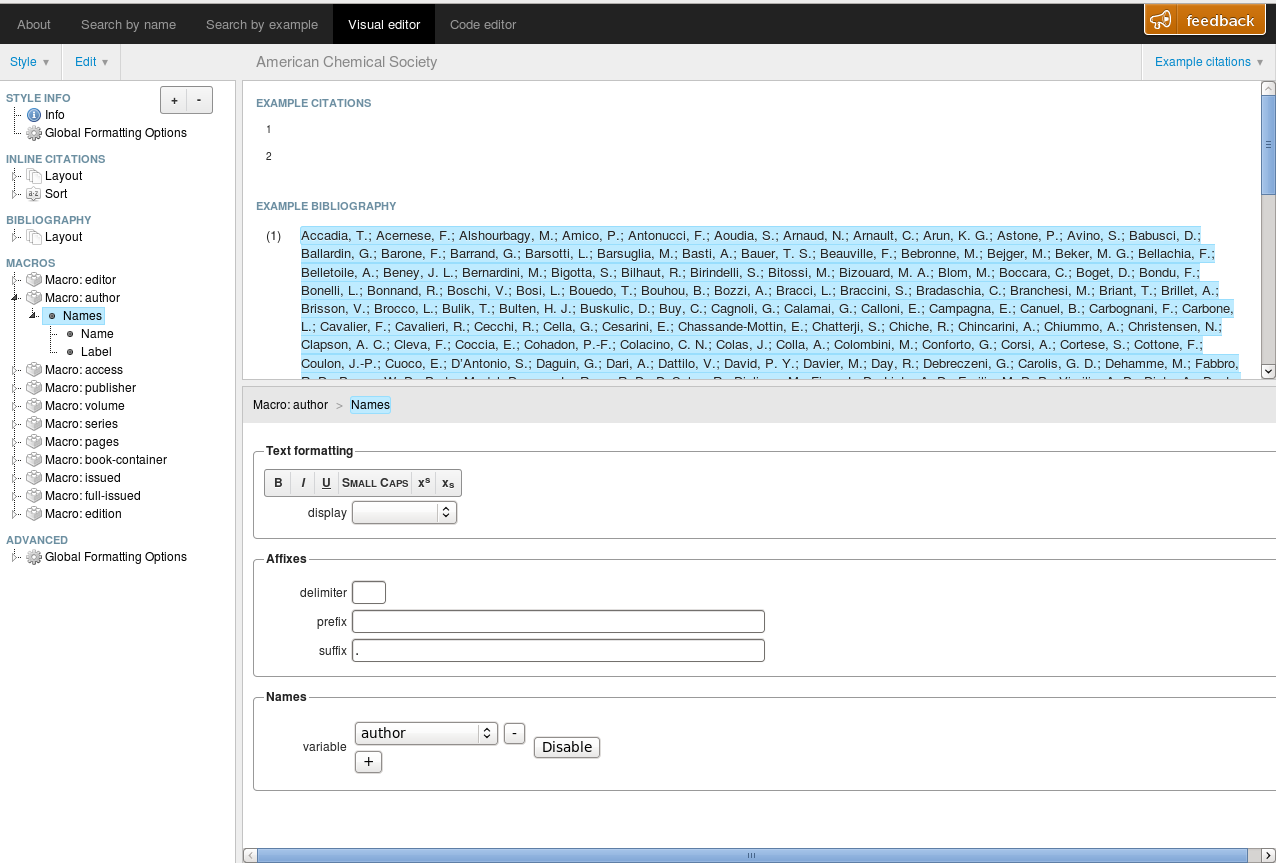
\includegraphics[scale=0.2]{11_2014_screen_editor.png}
  \caption{Акно візуальнага рэдактара: фарматаванне імёнаў аўтараў}
\end{figure}

\subsection*{Практычнае выкарыстанне}

Zotero рэалізаваны ў выглядзе плагіна для Firefox (найбольш поўнафункцыянальны) ды standalone"=праграмы.

\subsubsection*{Напаўненне базы бібліяграфіі}

Найбольш тыповы і зручны спосаб для артыкулаў: зайсці на старонку з анатацыяй адпаведнага артыкулу на афіцыйным сайце часопісу і націснуць кнопку захавання спасылкі (рыс. 2).

Для кніг: ўвесці ISBN.

\subsubsection*{Кіраванне базай}

Спасылкі сартуюцца па тэках (адна спасылка можа знаходзіцца ў некалькіх тэках). Акно плагіна адлюстроўвае спіс тэкаў, спіс спасылак у абранай тэцы ды падрабязнасці абранай спасылкі (рыс. 1). Магчымы хуткі пошук па зместу спасылак.


\begin{figure}[h!]
  \centering
  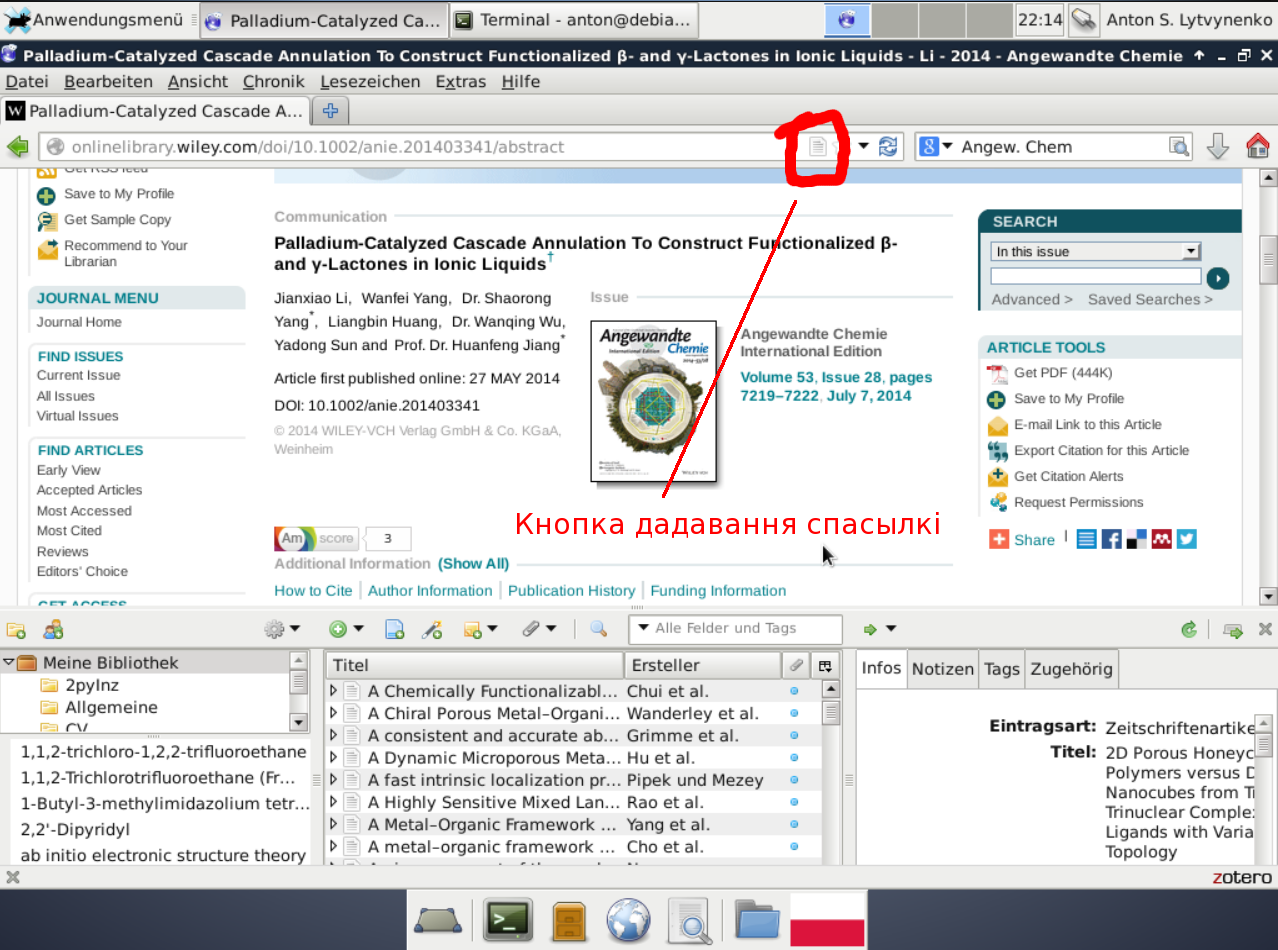
\includegraphics[scale=0.2]{11_2014_Fig1.png}
  \caption{Панэль Firefox"=плагіна Zotero і аўтаматычнае дадаванне спасылкі са старонкі часопіса Angewandte Chemie}
\end{figure}



\subsubsection*{Дадаванне спасылкі ў тэкст}

Інтэграцыйны плагін дадае кнопкі ў панэль офіснага працэсара (рыс. 3): дадаць спасылку (пад час першага выкарыстання прапануецца выбраць шаблон фарматавання), рэдагаваць спасылку, дадаць спіс літаратуры, рэдагаваць спіс літаратуры, панавіць спіс, усталяваць опцыі для дакуманту, выдаліць коды палёў (пераўтварае фарматаваныя спасылкі ў звыклы тэкст). Устаўка ды рэдагаванне магчымае праз выбар спасылак са спісаў, а таксама праз хуткі пошук у акенцы дадавання (рыс. 4) Выдаленне спасылкі "--- праз выдаленне адпаведнага аб’екту ў тэксце.



\begin{figure}[h!]
  \centering
  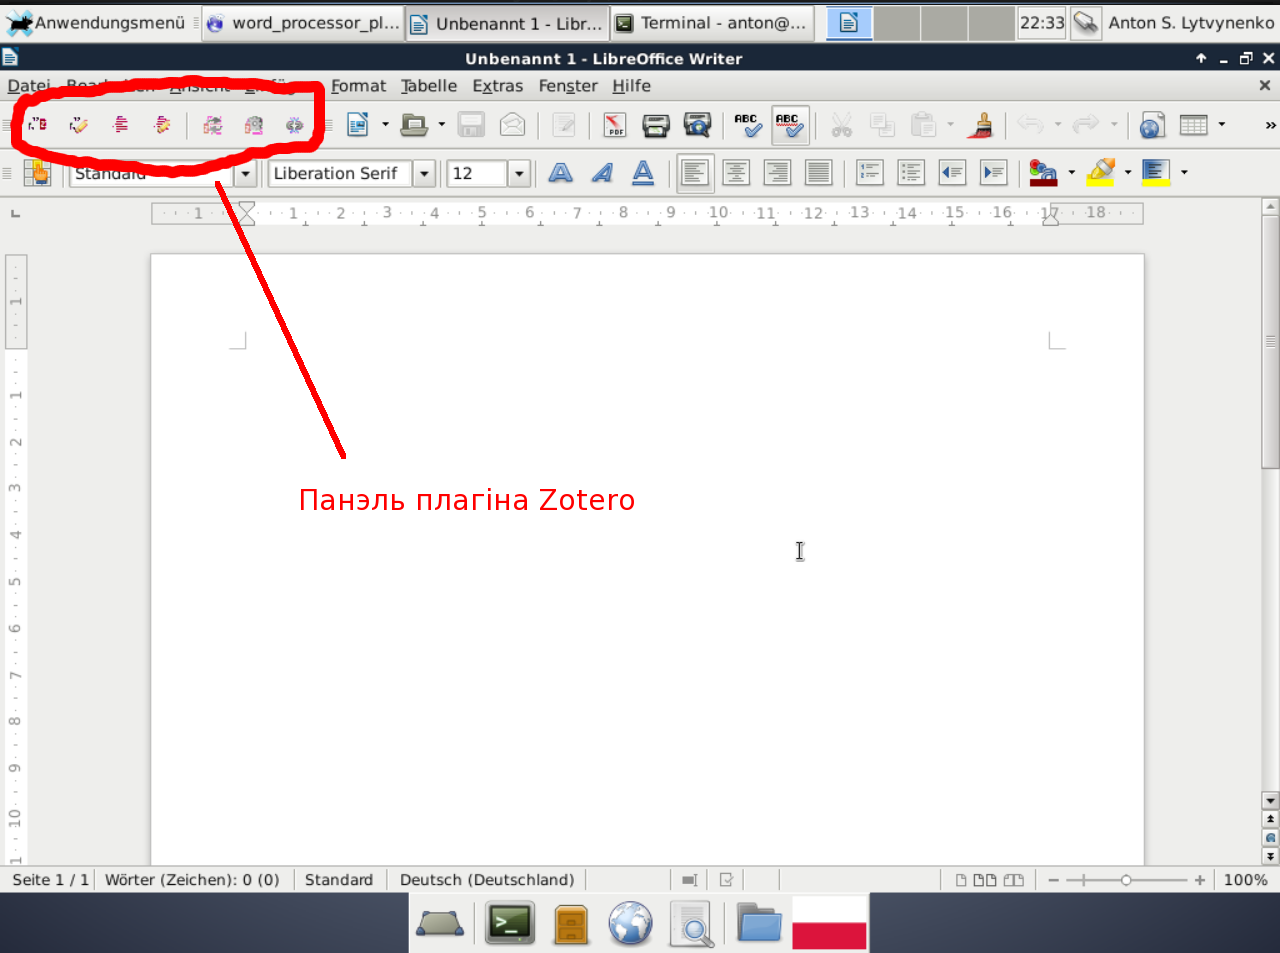
\includegraphics[scale=0.2]{11_2014_Fig2.png}
  \caption{Інтэграцыя Zotero ў LibreOffice}
\end{figure}


\begin{figure}[h!]
  \centering
  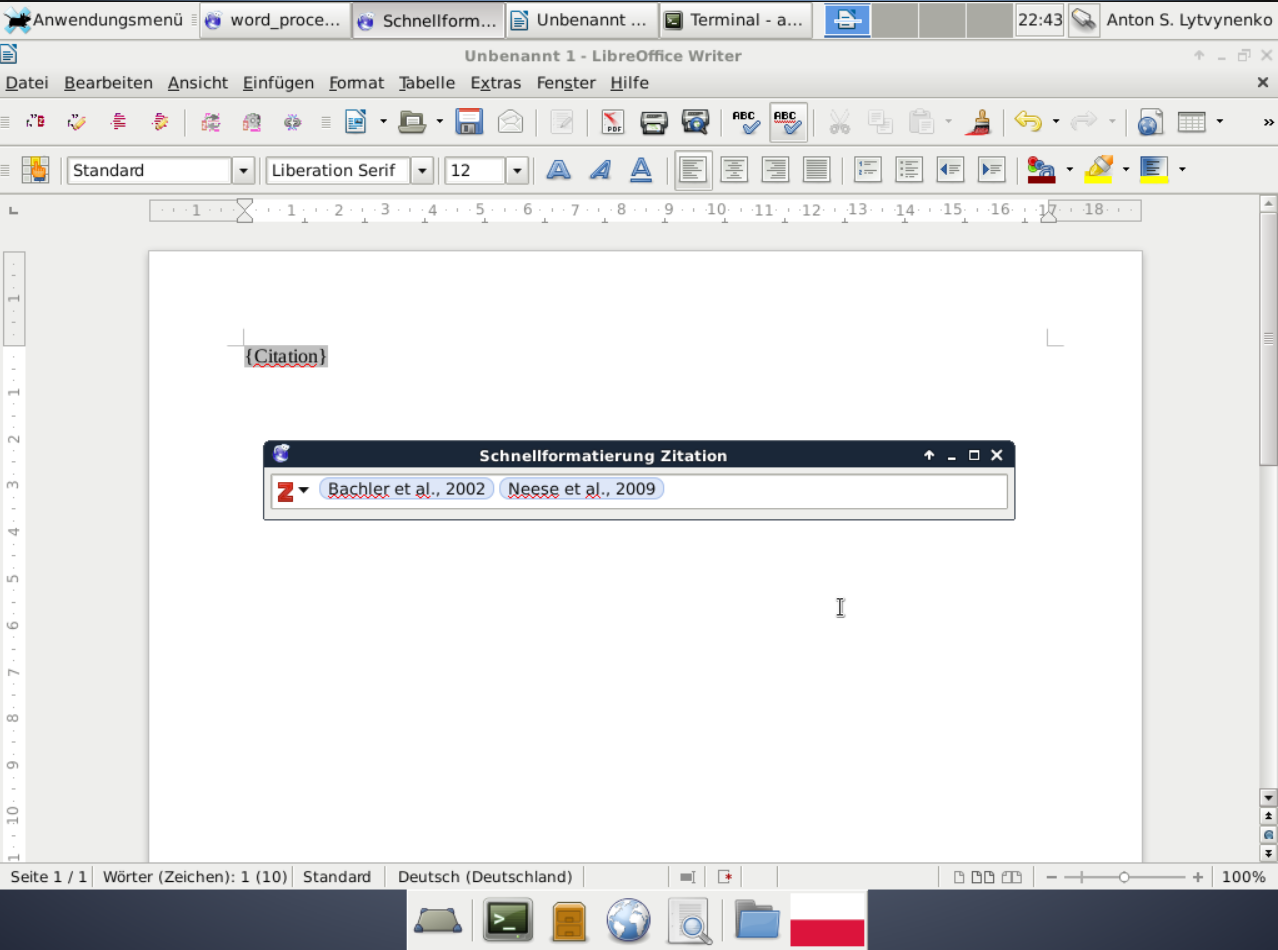
\includegraphics[scale=0.2]{11_2014_Fig3.png}
  \caption{Устаўка спасылкі хуткім пошукам}
\end{figure}

\subsection*{Палі і закладкі. Copy/Paste/Delete. Абмен \linebreak Open/Libre Office ды MS}

Zotero можа захоўваць дадзеныя пра спасылку ў зносках/палях альбо закладках. Варыянт закладак забяспечвае сумяшчальнасць пры супольнай працы ў OpenOffice ды MS Word, але не дазваляе аперацыі капіявання"=ўстаўкі над спасылкамі ў тэксце. Больш стандартным рэжымам з’яўляецца выкарыстанне зносак/палёў, якія дазваляюць працу са спасылкамі як са звыклымі элементамі тэксту "--- капіяванне, ўстаўка, перанос (у тым ліку з файлу ў файл).

\subsection*{Некаторыя брудныя падрабязнасці}

Іншы раз Zotero праз тыя ці іншыя прычыны фарматуе спасылку няправільна. Асабліва часта гэта стаецца пры наяўнасці ў спасылцы верхніх і ніжніх індэксаў, якія адлюстроўваюцца без адпаведнага фарматавання. Магчымасць «рэдагаваць бібліяграфію» дазваляе адфарматаваць тэкст спасылкі ў спісе літаратуры ўручную. Пры гэтым яе тэкст (а таксама нумар, зазначаны ў спісе літаратуры) прыпыняе абнаўляцца аўтаматычна (нумар у асноўным тэксце абнаўляецца) "--- пажадана не забыцца на гэта ў фінальнай версіі дакуманта.

Магчымасць ручнога фарматавання дае таксама магчымасць розных нестандартных спасылак (напрыклад, кампазітнай спасылкі, пры якой пад адным нумарам цытуецца некалькі спасылак (a, b, \ldots{})). Карыстальнік можа спачатку згенераваць праз сістэму індывідуальныя спасылкі, пасля стварыць спасылку на нейкі dummy"=аб’ект (напрыклад, нататку), спаслацца на яго і адфарматаваць тэкст уручную, ўставіўшы згенераваны тэкст пасля адпаведнага рэдагавання.

Над дакументам, у які з дапамогай Zotero ўстаўленыя спасылкі, можна працаваць і на кампутарах, дзе Zotero не ўсталявана, ў тым ліку ў версіях рэдактараў, якія не падтрымліваюцца Zotero (напрыклад, MS Word раней за версію 2003), ў тым ліку выконваць аперацыі капіявання, пераносу ці выдалення спасылак у тэксце. Пасля рэдагавання на такой сістэме дастаткова адчыніць дакумант у сістэме з усталяваным Zotero і панавіць бібліяграфію.

\subsection*{Высновы}

FLOSS"=сістэма Zotero, што інтэгруецца ў папулярныя офісныя тэкставыя працэсары, дазваляе аўтаматычнае фарматаванне і перанумероўку спасылак на літаратурныя крыніцы, што істотна палягшае працу навукоўцаў пры афармленні вынікаў іхняе працы. У адрозненні ад працы BibTeX і заснаваных на ім сістэм, Zotero дапоўненая кампанентамі аўтаматызаванага збору ды арганізацыі бібліяграфічных спасылак, што з’яўляецца мэтазгодным для \linebreak WYSIWYG"=сістэмы і таксама палягшае працу.

\begin{thebibliography}{9}
\bibitem{Litvinenko1} \url{http://citationstyles.org/}
\bibitem{Litvinenko2} \url{https://www.zotero.org/styles}
\bibitem{Litvinenko3} \url{http://editor.citationstyles.org/searchByExample/}
\end{thebibliography}
\end{document}

\documentclass[10pt, a5paper]{article}
\usepackage{pdfpages}
\usepackage{parallel}
\usepackage[T2A]{fontenc}
\usepackage{ucs}
\usepackage[utf8x]{inputenc}
\usepackage[polish,english,russian]{babel}
\usepackage{hyperref}
\usepackage{rotating}
\usepackage[inner=2cm,top=1.8cm,outer=2cm,bottom=2.3cm,nohead]{geometry}
\usepackage{listings}
\usepackage{graphicx}
\usepackage{wrapfig}
\usepackage{longtable}
\usepackage{indentfirst}
\usepackage{array}
\newcolumntype{P}[1]{>{\raggedright\arraybackslash}p{#1}}
\frenchspacing
\usepackage{fixltx2e} %text sub- and superscripts
\usepackage{icomma} % коскі ў матэматычным рэжыме
\PreloadUnicodePage{4}

\newcommand{\longpage}{\enlargethispage{\baselineskip}}
\newcommand{\shortpage}{\enlargethispage{-\baselineskip}}

\def\switchlang#1{\expandafter\csname switchlang#1\endcsname}
\def\switchlangbe{
\let\saverefname=\refname%
\def\refname{Літаратура}%
\def\figurename{Іл.}%
}
\def\switchlangen{
\let\saverefname=\refname%
\def\refname{References}%
\def\figurename{Fig.}%
}
\def\switchlangru{
\let\saverefname=\refname%
\let\savefigurename=\figurename%
\def\refname{Литература}%
\def\figurename{Рис.}%
}

\hyphenation{admi-ni-stra-tive}
\hyphenation{ex-pe-ri-ence}
\hyphenation{fle-xi-bi-li-ty}
\hyphenation{Py-thon}
\hyphenation{ma-the-ma-ti-cal}
\hyphenation{re-ported}
\hyphenation{imp-le-menta-tions}
\hyphenation{pro-vides}
\hyphenation{en-gi-neering}
\hyphenation{com-pa-ti-bi-li-ty}
\hyphenation{im-pos-sible}
\hyphenation{desk-top}
\hyphenation{elec-tro-nic}
\hyphenation{com-pa-ny}
\hyphenation{de-ve-lop-ment}
\hyphenation{de-ve-loping}
\hyphenation{de-ve-lop}
\hyphenation{da-ta-ba-se}
\hyphenation{plat-forms}
\hyphenation{or-ga-ni-za-tion}
\hyphenation{pro-gramming}
\hyphenation{in-stru-ments}
\hyphenation{Li-nux}
\hyphenation{sour-ce}
\hyphenation{en-vi-ron-ment}
\hyphenation{Te-le-pathy}
\hyphenation{Li-nux-ov-ka}
\hyphenation{Open-BSD}
\hyphenation{Free-BSD}
\hyphenation{men-ti-on-ed}
\hyphenation{app-li-ca-tion}

\def\progref!#1!{\texttt{#1}}
\renewcommand{\arraystretch}{2} %Іначай формулы ў матрыцы зліпаюцца з лініямі
\usepackage{array}

\def\interview #1 (#2), #3, #4, #5\par{

\section[#1, #3, #4]{#1 -- #3, #4}
\def\qname{LVEE}
\def\aname{#1}
\def\q ##1\par{{\noindent \bf \qname: ##1 }\par}
\def\a{{\noindent \bf \aname: } \def\qname{L}\def\aname{#2}}
}

\def\interview* #1 (#2), #3, #4, #5\par{

\section*{#1\\{\small\rm #3, #4. #5}}

\def\qname{LVEE}
\def\aname{#1}
\def\q ##1\par{{\noindent \bf \qname: ##1 }\par}
\def\a{{\noindent \bf \aname: } \def\qname{L}\def\aname{#2}}
}

\begin{document}
\title{Применение популярных протоколов и свободного ПО в управлении мобильным роботом}
\author{Андрей Дунец "--- Брест, Беларусь\footnote{\url{dunets@gmail.com}, \url{http://lvee.org/ru/abstracts/143}}}
\maketitle
\begin{abstract}
We consider the problems of telemetry, positioning and cont\-rol of the mobile robot for rivers and lakes monitoring. The project uses Bluetooth technology to transmit the telemetry data. RTKLIB library implementation of Real"=Time Kinematic algo\-rithm is used for positioning. Current version of the control system is based on the Ardupilot project.
\end{abstract}
Мониторинг водоемов актуален для решения самых разных задач. Начиная от построения профиля дна водоема для прогнозирования паводков и обеспечения безопасности судоходства и заканчивая контролем состояния воды в интересах рыболовецких хозяйств и служб охраны природных ресурсов. Применение мобильных водоплавающих роботов позволяет автоматизировать процесс мониторинга и значительно снизить его себестоимость.

На данный момент робот и его система управления находится в разработке. Текущие решаемые задачи это телеметрия, позиционирование и управление роботом.

Телеметрия обязательная часть подобного комплекса, так как без неё нормальная разработка ПО и отладка оборудования сильно затруднена. Выбор был сделан с расчетом на доступные популярные решения, так как особенности этих технологий хорошо известны и они недороги в отличии от решений, которые основаны на закрытых протоколах.

Первоначальным вариантом было использование Bluetooth \linebreak Class~1. Заявленная дальность до 100 метров, дешевизна оборудования, простота настройки позволили поставить несколько экспериментов по передаче телеметрических данных. Использовался профиль SPP (Serial Port Profile). На стороне робота микроконтроллер автопилота связывался с компьютером через Bluetooth модем BTM"=222, который полностью реализует весть стек необходимых беспроводных протоколов профиля SPP, предоставляет TTL UART"=интерфейс и управляется AT"=командами. На стороне компьютера применялся встроенный адаптер Bluetooth. Выяснилось, что приемо"=передатчики, кроме заявленных характеристик должны быть оснащены соответствующими антеннами. Удалось использовать на стороне робота антенну от адаптера WiFi (частотный диапазон один и тот же) и практическая полученная дальность составила 30 метров.

Эксперименты показали, что Bluetooth можно использовать для передачи телеметрической информации на небольшие расстояния. Но профиль SPP, будучи простым в использовании, позволяет передавать только один поток данных. На практике нужно как минимум два потока: поток с приемника GPS и поток консоли. Можно использовать протокол, который поддерживает подобное мультиплексирование. Возможны так же экзотические варианты: пробросить TCP трафик через PPP.

Дополнительно выявились проблемы с восстановлением связи при утере соединения: пересопряжение устройств требует поддержки в прикладном ПО, что неудобно. Сейчас как наиболее оптимальное решение для следующего шага рассматривается переход на WiFi.
WiFi обеспечит большую скорость передачи данных. Можно использовать более мощные антенны. Штатно доступный стек\linebreak TCP/IP позволит мультиплексировать данные. При этом возрастет энергопотребление, что является минусом данного решения. Эксперименты покажут, какой вариант наиболее оптимален.

Для позиционирования робота в акватории водоема применяется GPS. Для уточнения координат используется алгоритм RTK (Real"=Time Kinematic), который реализован в открытой библиотеке RTKLIB (\url{rtklib.com}). Для получения данных GPS применяется приемник NEO"=6M фирмы u"=blox и штатные утилиты из состава RTKLIB. Приемник настраивается с помощью хаков, разработанных сообществом OpenStreetMap. БД корректировок берутся с серверов проекта IAG Reference Frame Sub"=Commission for Europe (\url{http://www.euref.eu/}), базовые станции которого находятся на достаточно близком расстоянии от Беларуси.

Первоначальное решение по управлению, на которое был сделан упор "--- использовать существующие автопилоты, в которых используется открытое ПО. Одним из таких проектов является APM Autopilot Suite (\url{http://ardupilot.com}). Его особенности:

\begin{itemize}
  \item открытые исходные тексты ПО автопилота и базовой станции (лицензия GNU GPL);
  \item базовые аппаратные решения основаны на открытой платформе Arduino (Atmel Atmega), но более продвинутые используют 32"=разрядные контроллеры ARM Cortex и платы с закрытым дизайном;
  \item активное сообщество пользователей DIY Drones, которые делятся наработками и обмениваются опытом (\url{diydrones.com});
  \item используется открытый протокол MAVLink (Micro Air Vehicle Communication Protocol, \\ \url{http://qgroundcontrol.org/mavlink/start});
  \item реализовано управление бесплотниками с разной кинематикой: несколько видов коптеров, вертолет, самолет, автомобиль, что положительно сказалось на архитектуре ПО: код представляет из себя несколько программ управления для разной кинематики и общую библиотеку алгоритмов;
  \item в алгоритмах доступно множество полезных решений для создания собственного автопилота: от драйверов устройств (датчики, исполнительные механизмы, телеметрия и т.п.) до математики (ПИД, фильтры Калмана и т.д.).
\end{itemize}

Был приобретен комплект оборудования APM 2.5 и поставлено несколько экспериментов программированию автопилота. Выяснилось, что хотя код написан довольно качественно, документирован он слабо и отлаживать на микроконтроллере сложную математику весьма трудоемко. Также оказалось, что решение на базе микроконтроллеров не подходит для задач управления с нашими требованиями по позиционированию. Для достижения автономности на борту должен быть 32"=разрядный компьютер с тактовой частотой в несколько сотен мегагерц, чтобы вести расчеты позиции по алгоритму RTK. На такой компьютер можно установить полноценную ОС, которая упростит остальные эксперименты. При этом от микроконтроллера для управления вводом/выводом нельзя отказываться, так как есть перечень задач, которые оптимально выполнять именно на нем. Сейчас рассматривается возможность дополнить бортовую вычислительную систему платой микрокомпьютера под управлением Linux. Выбор будет сделан из двух вариантов: Raspberry Pi и Beagle Bone Black. Скорее всего, выбор будет остановлен на Rapberry Pi, так как у этой платы проще подсистема питания, что упрощает стыковку со штатным аккумулятором робота.

Результаты экспериментов доступны на Bitbucket:\\ \url{https://bitbucket.org/pondskaterteam/pondskater}


\end{document}



\documentclass[10pt, a5paper]{article}
\usepackage{pdfpages}
\usepackage{parallel}
\usepackage[T2A]{fontenc}
\usepackage{ucs}
\usepackage[utf8x]{inputenc}
\usepackage[polish,english,russian]{babel}
\usepackage{hyperref}
\usepackage{rotating}
\usepackage[inner=2cm,top=1.8cm,outer=2cm,bottom=2.3cm,nohead]{geometry}
\usepackage{listings}
\usepackage{graphicx}
\usepackage{wrapfig}
\usepackage{longtable}
\usepackage{indentfirst}
\usepackage{array}
\newcolumntype{P}[1]{>{\raggedright\arraybackslash}p{#1}}
\frenchspacing
\usepackage{fixltx2e} %text sub- and superscripts
\usepackage{icomma} % коскі ў матэматычным рэжыме
\PreloadUnicodePage{4}

\newcommand{\longpage}{\enlargethispage{\baselineskip}}
\newcommand{\shortpage}{\enlargethispage{-\baselineskip}}

\def\switchlang#1{\expandafter\csname switchlang#1\endcsname}
\def\switchlangbe{
\let\saverefname=\refname%
\def\refname{Літаратура}%
\def\figurename{Іл.}%
}
\def\switchlangen{
\let\saverefname=\refname%
\def\refname{References}%
\def\figurename{Fig.}%
}
\def\switchlangru{
\let\saverefname=\refname%
\let\savefigurename=\figurename%
\def\refname{Литература}%
\def\figurename{Рис.}%
}

\hyphenation{admi-ni-stra-tive}
\hyphenation{ex-pe-ri-ence}
\hyphenation{fle-xi-bi-li-ty}
\hyphenation{Py-thon}
\hyphenation{ma-the-ma-ti-cal}
\hyphenation{re-ported}
\hyphenation{imp-le-menta-tions}
\hyphenation{pro-vides}
\hyphenation{en-gi-neering}
\hyphenation{com-pa-ti-bi-li-ty}
\hyphenation{im-pos-sible}
\hyphenation{desk-top}
\hyphenation{elec-tro-nic}
\hyphenation{com-pa-ny}
\hyphenation{de-ve-lop-ment}
\hyphenation{de-ve-loping}
\hyphenation{de-ve-lop}
\hyphenation{da-ta-ba-se}
\hyphenation{plat-forms}
\hyphenation{or-ga-ni-za-tion}
\hyphenation{pro-gramming}
\hyphenation{in-stru-ments}
\hyphenation{Li-nux}
\hyphenation{sour-ce}
\hyphenation{en-vi-ron-ment}
\hyphenation{Te-le-pathy}
\hyphenation{Li-nux-ov-ka}
\hyphenation{Open-BSD}
\hyphenation{Free-BSD}
\hyphenation{men-ti-on-ed}
\hyphenation{app-li-ca-tion}

\def\progref!#1!{\texttt{#1}}
\renewcommand{\arraystretch}{2} %Іначай формулы ў матрыцы зліпаюцца з лініямі
\usepackage{array}

\def\interview #1 (#2), #3, #4, #5\par{

\section[#1, #3, #4]{#1 -- #3, #4}
\def\qname{LVEE}
\def\aname{#1}
\def\q ##1\par{{\noindent \bf \qname: ##1 }\par}
\def\a{{\noindent \bf \aname: } \def\qname{L}\def\aname{#2}}
}

\def\interview* #1 (#2), #3, #4, #5\par{

\section*{#1\\{\small\rm #3, #4. #5}}

\def\qname{LVEE}
\def\aname{#1}
\def\q ##1\par{{\noindent \bf \qname: ##1 }\par}
\def\a{{\noindent \bf \aname: } \def\qname{L}\def\aname{#2}}
}

\begin{document}
\title{Smart GreenHouse}
\author{Дмитрий Ясевич, Василий Слапик, Павет Вервенко, \\
Дмитрий Огиевич, Минск, Беларусь\footnote{\url{dzmitry_yasevich@epam.com}, \url{http://lvee.org/ru/abstracts/131}}}
\maketitle
\begin{abstract}
«Java for Farmers»: Greenhouse monitoring and automation, using Java, Raspberry Pi, Linux and multiple sensors. Smart Greenhouse Project is a Oracle IoT winner 2014 in professional category.
\end{abstract}
\subsection*{История проекта}

Ни для кого не секрет, что «умные» программные решения (дома, парники, и т.\,д.) находят все большее применение в реальном мире. Узнав о существовании Java Embedded для создания «Интернета вещей», мы загорелись идеей попробовать ее в деле. После недолгого обсуждения в качестве объекта для экспериментов была выбрана «умная» теплица.

Причин было несколько. Первая из них "--- умными домами занимаются широкий круг инженеров и энтузиастов, начиная от студенческих клубов и заканчивая серьезными IT-компаниями, поэтому здесь было тяжело создать что-то действительно новое и интересное.

Вторая, но не менее значимая причина, заключается в том, что Беларусь "--- это страна, в которой хорошо развит аграрный сектор. Наша команда решила быть патриотичной и создать устройство достаточно простое, но при этом потенциально полезное для использования в сельском хозяйстве. Таким образом выбор пал на теплицу, как точку приложения наших сил.

\subsection*{Java Embedded}

Java уже успела зарекомендовать себя в качестве успешной платформы для решения множества задач, включая и «умные» системы. Если охватывать весь спектр техники, то можно насчиать более 10 млрд устройств, использующих Java. При этом подавляющая часть таких устройств так или иначе базируются на *nix платформах.

Почему все-таки стоит использовать Java для встраиваемых систем; ведь на первый взгляд у Java недостатков гораздо больше, чем преимуществ:

\begin{itemize}
  \item Java является одной из самых популярных платформ для разработки приложений;
  \item Оптимизирована для Embedded решений;
  \item Высокопроизводительные, переносимые приложения;
  \item Свободно распространяемые инструменты разработчика;
  \item Проверенная модель безопасности.
\end{itemize}

Как показала практика, для создания «умной» теплицы с помощью Java Embedded достаточно скромных ресурсов Raspberry Pi, работающей под управлением Linux.

\subsection*{Функциональные возможности теплицы}

К числу основных особенностей проекта относятся:

\begin{itemize}
  \item Контроль и управление светом.
  \item Контроль полива.
  \item Контроль температуры и влажности.
  \item Удаленный мониторинг текущего состояния теплицы.
  \item Автоматическое управление теплицей.
  \item Автоматический процесс фотографирования роста растений.
  \item Низкая потребляемая мощность.
  \item Защита от коротких замыканий и отключения электричества.
\end{itemize}

Таким образом, наша разработка на данный момент представляет собой полнофункциональную автоматизированную систему, которая позволяет выращивать комнатные растения, сохраняя душевное спокойствие владельца теплицы. Обеспечивается удаленное управление и мониторинг света, температуры и влажности. Также запланирована возможность дистанционной проверки текущего процесса роста в режиме онлайн.

\subsection*{Реализация}

При создании нашего проекта мы старались использовать открытые и свободные компоненты и технологии: Raspberry Pi, Java Embedded, Raspbian, pi4j, Jetty и нескольких сенсоров.

Электрическая схема Smart GreenHouse показана на рисунке.

\begin{figure}[h!]
  \centering
  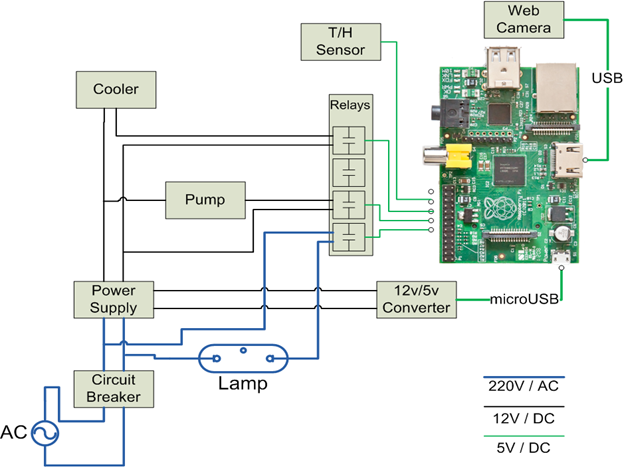
\includegraphics[scale=0.8]{13_2014_1.png}
\end{figure}

Raspbian "--- это операционная система, основанная на Debian и оптимизированная для Raspberry Pi, а pi4j "--- библиотека для работы с аппаратной частью Raspberry Pi.

Ниже приведен пример кода на Java для датчика влажности и температуры при использовании pi4j:

\begin{verbatim}
// инициализация
GpioController gpio = GpioFactory.getInstance();
GpioPinDigitalOutput light = 
	gpio.provisionDigitalOutputPin(
	RaspiPin.GPIO_07, "Light", PinState.LOW); 
	// подключились к пину 7
	
light.setShutdownOptions(true, PinState.LOW, 
	PinPullResistance.OFF); /* задали опцию, чтоб на выходе 
	из приложения этот пин отключался (чтоб свет гас) */

// управление
light.high(); // включить пин
light.low(); // выключить
\end{verbatim}
\subsection*{Текущий статус и планы}

На данный момент проект все еще развивается "--- добавляем поддержку разных датчиков, решаем проблемы, возникающие при совместной работе нескольких таких устройств. 
Также создаем специализированный дистрибутив на базе Yocto Project, содержащий все необходимое для работы автоматизированной теплицы «из коробки».

Полный исходный код управляющей части проекта доступен по адресу \url{https://bitbucket.org/Temdegon/greenhouse}

\end{document}

\documentclass[10pt, a5paper]{article}
\usepackage{pdfpages}
\usepackage{parallel}
\usepackage[T2A]{fontenc}
\usepackage{ucs}
\usepackage[utf8x]{inputenc}
\usepackage[polish,english,russian]{babel}
\usepackage{hyperref}
\usepackage{rotating}
\usepackage[inner=2cm,top=1.8cm,outer=2cm,bottom=2.3cm,nohead]{geometry}
\usepackage{listings}
\usepackage{graphicx}
\usepackage{wrapfig}
\usepackage{longtable}
\usepackage{indentfirst}
\usepackage{array}
\newcolumntype{P}[1]{>{\raggedright\arraybackslash}p{#1}}
\frenchspacing
\usepackage{fixltx2e} %text sub- and superscripts
\usepackage{icomma} % коскі ў матэматычным рэжыме
\PreloadUnicodePage{4}

\newcommand{\longpage}{\enlargethispage{\baselineskip}}
\newcommand{\shortpage}{\enlargethispage{-\baselineskip}}

\def\switchlang#1{\expandafter\csname switchlang#1\endcsname}
\def\switchlangbe{
\let\saverefname=\refname%
\def\refname{Літаратура}%
\def\figurename{Іл.}%
}
\def\switchlangen{
\let\saverefname=\refname%
\def\refname{References}%
\def\figurename{Fig.}%
}
\def\switchlangru{
\let\saverefname=\refname%
\let\savefigurename=\figurename%
\def\refname{Литература}%
\def\figurename{Рис.}%
}

\hyphenation{admi-ni-stra-tive}
\hyphenation{ex-pe-ri-ence}
\hyphenation{fle-xi-bi-li-ty}
\hyphenation{Py-thon}
\hyphenation{ma-the-ma-ti-cal}
\hyphenation{re-ported}
\hyphenation{imp-le-menta-tions}
\hyphenation{pro-vides}
\hyphenation{en-gi-neering}
\hyphenation{com-pa-ti-bi-li-ty}
\hyphenation{im-pos-sible}
\hyphenation{desk-top}
\hyphenation{elec-tro-nic}
\hyphenation{com-pa-ny}
\hyphenation{de-ve-lop-ment}
\hyphenation{de-ve-loping}
\hyphenation{de-ve-lop}
\hyphenation{da-ta-ba-se}
\hyphenation{plat-forms}
\hyphenation{or-ga-ni-za-tion}
\hyphenation{pro-gramming}
\hyphenation{in-stru-ments}
\hyphenation{Li-nux}
\hyphenation{sour-ce}
\hyphenation{en-vi-ron-ment}
\hyphenation{Te-le-pathy}
\hyphenation{Li-nux-ov-ka}
\hyphenation{Open-BSD}
\hyphenation{Free-BSD}
\hyphenation{men-ti-on-ed}
\hyphenation{app-li-ca-tion}

\def\progref!#1!{\texttt{#1}}
\renewcommand{\arraystretch}{2} %Іначай формулы ў матрыцы зліпаюцца з лініямі
\usepackage{array}

\def\interview #1 (#2), #3, #4, #5\par{

\section[#1, #3, #4]{#1 -- #3, #4}
\def\qname{LVEE}
\def\aname{#1}
\def\q ##1\par{{\noindent \bf \qname: ##1 }\par}
\def\a{{\noindent \bf \aname: } \def\qname{L}\def\aname{#2}}
}

\def\interview* #1 (#2), #3, #4, #5\par{

\section*{#1\\{\small\rm #3, #4. #5}}

\def\qname{LVEE}
\def\aname{#1}
\def\q ##1\par{{\noindent \bf \qname: ##1 }\par}
\def\a{{\noindent \bf \aname: } \def\qname{L}\def\aname{#2}}
}

\begin{document}
\title{clsync progess: security and porting to FreeBSD}
\author{Dmitry Okunev "--- Moscow, Russia\footnote{\url{xaionaro@gmail.com}, \url{http://lvee.org/ru/abstracts/138}}}
\maketitle
\begin{abstract}
The report focuses on methods to increase a level of security of "clsync" (free live sync utility). Multiple approaches to reduce risks of attack were used, and practical experience of applying these approaches is given. Used methods include unsharing un\-necessary resources, splitting the process to privileged and non"=privileged threads and using Linux"=specific security"=related API. Also problems of porting Linux"=based clsync to FreeBSD are described, including variants and problems of FS monitoring in FreeBSD.
\end{abstract}
\subsection*{Введение}

Проект clsync возник как альтернативный высокопроизводи"=\linebreak тельный инструмент для синхронизации контейнеров LXC между узлами HA"=кластера и их резервного копирования, изначально ориентированный под внутренние нужды отдела UNIX"=технологий НИЯУ МИФИ \cite{Okunev1}, \cite{Okunev2}. Данная статья является отчётом о достижениях по развитию программы «clsync» в вопросах повышения уровня безопасности и портируемости на другие ОС в 2014 году.

\subsection*{Средства защиты}

Процесс отслеживания изменений на ФС часто требует  привилегий root (или capability ``CAP\_DAC\_READ\_SEARCH'' \cite{Okunev3} в Linux). Однако известные программы \cite{Okunev4} для синхронизации на базе inotify \cite{Okunev5} имеют достаточно малое сообщество и при этом не имеют никаких встроенных механизмов повышения безопасности (сброс лишних привилегий, namespaces и т.п.). В результате становится маловозможной настройка синхронизации посредством inotify в системах, требующих особой защиты. Далее будут рассмотрены средства для минимизации последствий эксплуатации уязвимостей, реализованные в «clsync» летом 2014"=го года.

\subsubsection*{Задача}

Задача заключается в минимизации последствий обнаружения и эксплуатации уязвимостей в clsync злоумышленником.

Предполагается, что:

\begin{itemize}
  \item Необходимо предоставить процессу «clsync» полный доступ к некоторому файловому дереву, содержащему объекты (файлы, директории и т.п.) с произвольными наборами прав.
  \item Злоумышленник имеет возможность управлять содержимым данного файлового дерева, но не имеет других путей для манипуляции над процессом «clsync».
  \item «clsync» не наблюдает за файлами, чтение которых злоумышленником привело бы к ущербу.
  \item Процессу «clsync» необходимо запускать внешний процесс (например «rsync») для осуществления синхронизации.
\end{itemize}

Практическим применением данной задачи является хостинг на базе LXC, требующий синхронизации на другой узел для реализации High Availability \cite{Okunev1, Okunev6}. А для синхронизации запускается по одному процессу «clsync» на каждый контейнер. В такой конфигурации содержимым контейнера управляют малодоверенные пользователи, которые могут иметь интерес выйти за пределы предоставленных им пространств имен (namespaces), эксплуатируя уязвимость в «clsync» (который в свою очередь запущен с хост"=системы, то есть извне пространств имен контейнера).

\subsubsection*{Решение}

В качестве мер для повышения безопасности предлагается:

\begin{itemize}
  \item Применить unshare() \cite{Okunev7} для отсоединения от пространств имен хост"=системы для сети, IPC и других ресурсов.
  \item Сбросить привилегии с помощью setuid()/setgid(), предварительно сохранив capability «CAP\_DAC\_READ\_SEARCH» \linebreak для сохранения полного доступа к файловому дереву.
  \item Производить chroot(), pivot\_root() \cite{Okunev8} и umount() для запрета доступа к файлам вне наблюдаемой директории.
  \item Разделять процесс на «большой непривилегированный» и «малый привилегированный».
  \item Использовать seccomp filter \cite{Okunev9} для запрета лишних системных вызовов (syscalls) внутри непривилегированного потока.
\end{itemize}

\paragraph{unshare().}

Применение unshare() позволяет запретить доступ к сети (и сервисам, работающим на localhost), IPC и другим ресурсам. Это необходимо, чтобы предотвратить взлом процессов по цепочке (когда злоумышленник пытается взламывать другие сервисы через уязвимость clsync).

\paragraph{Сброс привилегий.}

Сброс привилегий "--- тривиальная и очень распространенная процедура. В «clsync» предлагается производить сброс с помощью setuid() и setgid() с предварительным сохранением capability «CAP\_DAC\_READ\_SEARCH» для доступа к файлам. Однако в рамках сформулированной задачи необходимо решить следующие проблемы:

\begin{enumerate}
  \item Запускаемому процессу для синхронизации (например, \linebreak «rsync») аналогично необходим доступ на чтение всего синхронизируемого файлового дерева. И наследовать для этого capability «CAP\_DAC\_READ\_SEARCH» недостаточно, так как кроме этого необходимо его активировать (добавить в effective capabilities bitmask). Но такого рода процессы обычно не имеют поддержки активации capabilities. Поэтому данную проблему необходимо решить возможностями «clsync». Для решения данной проблемы можно либо добавить в связку sudo (или аналог), или делать setuid()/setgid() назад на root. Использование дополнительного ПО существенно снижает уровень безопасности, поэтому setuid()/setgid() является более желательным вариантом. Но сохранение capabilities «CAP\_SETUID» и «CAP\_SETGID» фактически полностью ликвидирует защиту за счёт сброса привилегий. Чтобы решить данную проблему предложен способ разделения процесса на «большой привилегированный» и «малый непривилегированный».
  \item «CAP\_DAC\_READ\_SEARCH» предоставляет доступ на чтение всех файлов, что недопустимо в рамках сформулированной задачи. В качестве решения проблемы предлагается использовать chroot(), pivot\_root() и umount().
\end{enumerate}

\paragraph{Namespace файлового дерева.}

Как уже говорилось, для запрета доступа к файлам вне наблюдаемой директории предлагается использовать pivot\_root(), chroot() и umount(). В автоматической форме это делается по следующему алгоритму:

\begin{enumerate}
  \item Открепление от namespace точек монтирования с помощью unshare().
  \item Монтирование chroot"=окружения в отдельную директорию с помощью bind (с опцией режима ``только на чтение'').
  \item Переход в данную директорию.
  \item Вызов pivot\_root() для последующего отмонтирования rootfs хост"=системы.
  \item Вызов chroot() на данную директорию.
  \item Отмонтирование старого rootfs (что спровоцирует каскадное отмонтирование всех лишних точек монтирования).
\end{enumerate}

Данный подход даёт возможность достаточно надёжно защитить лишние файлы от чтения/изменения процессом «clsync». Однако существует риск, вызванный уязвимостью, описанной в статье \cite{Okunev10}. Данная проблема решается за счёт разделения процесса на «большой непривилегированный» и «малый привилегированный».

\paragraph{Splitting.}

Технически разделение процесса «clsync» на «большой непривилегированный» и «малый привилегированный» предполагает запуск дополнительного потока (thread) для обращения к системным вызовам, требующим привилегий выше чем «nobody». С точки зрения безопасности, это способ многократно снизить площадь для атаки на clsync. Если предположить, что потенциальные уязвимости распределены по всему коду равномерно, то данный подход позволяет ликвидировать последствия взлома почти полностью для более чем 90\% уязвимостей, и чем меньше будет код привилегированного потока, тем выше окажется эффективность метода. Однако данный подход требует применения блокировок и передачи сообщений между потоками, что существенно снижает производительность (время выполнения увеличивалось в несколько раз).

Для уменьшения потерь производительности был реализован механизм блокировок, комбинирующий pthread\_mutex\_* и spinlock, что позволило достичь на многоядерных системах времени выполнения близкого к прежнему (без данного разделения потоков), но со значительно большим расходом ресурсов CPU.

Однако, так как разделение производится при помощи pthread, то у непривилегированного потока есть доступ ко всей памяти привилегированного потока, включая доступ к stack и т.п. Это позволяет без особых сложностей провести атаку на привилегированный поток из непривилегированного. Чтобы решить данную проблему, предлагается использовать seccomp filter для запрета вызова mprotect из непривилегированного потока, а также «забыть» максимальное количество информации о привилегированном потоке. Если первое является реальным средством защиты, то второе "--- лишь способ усложнить эксплуатацию потенциальной уязвимости.

\paragraph{Seccomp.}

Seccomp, как уже было сказано выше, предлагается использовать для фильтрации лишних системных вызовов для непривилегированного потока, что позволяет:

\begin{itemize}
  \item защитить привилегированный поток с помощью mprotect \cite{Okunev11}.
  \item дополнительно снизить последствия эксплуатации уязвимости, так как набор действий злоумышленника будет ограничен до конкретного короткого списка системных вызовов.
\end{itemize}

\subsection*{Портирование на FreeBSD}

FreeBSD (как и другие BSD"=системы) до сих пор активно используются для реализации различных сервисов высокой доступности, однако в стандартном дереве портов данной ОС не предоставляется никаких production"=ready решений для живой синхронизации файлов (без использования специальных файловых систем). Далее будет описаны основные проблемы при портировании программы для живой синхронизации «clsync» под FreeBSD.

Оригинальный «clsync» использует inotify для наблюдения за ФС, однако данный API специфичен для Linux и не предоставляется во FreeBSD. В результате при портировании в качестве альтернатив для наблюдения за событями на ФС были выбраны «kqueue» \cite{Okunev12}, «bsm» \cite{Okunev13} и «dtrace» \cite{Okunev14}.

Основными проблемами при использовании «kqueue» являются:

\begin{itemize}
  \item использование большого количества файловых дескрипторов (в сравнении с inotify);
  \item невозможность получать детали по создаваемым файлами и директориям (что было решено полным пересканированием директории при появлении в ней нового объекта);
  \item необходимость «вручную» вычислять переносы файлов и директорий (и различать их с созданием жестких ссылок, т.е. hard links);
  \item множество сложноучитываемых эффектов (например, необходимо учитывать, что нельзя открывать pipes).
\end{itemize}

Основной проблемой при использовании «bsm» является требование глобальной перенастройки auditd.

А «dtrace», как выяснилось в ходе реализации его поддержки в «clsync», реализован не в соответствии с оригинальным «dtrace» \cite{Okunev15}. Причем различия построенным таким образом, что становится очень затруднительным получить полный путь файла, которому соответствует пойманное событие. В результате, реализация «dtrace» во FreeBSD непригодна для наблюдения за событиями ФС.

На данный момент самая стабильная работа clsync во FreeBSD обеспечена с применением библиотеки libinotify"=kqueue \cite{Okunev16}, которая представляет собой реализацию API inotify на базе kqueue.

\begin{thebibliography}{9}
  \bibitem{Okunev1} Окунев Д.Ю. «clsync — live sync utility», материалы Международная конференция разработчиков и пользователей свободного программного обеспечения Linux Vacation / Eastern Europe (LVEE Winter 2014), \url{http://lvee.org/en/reports/materials_lvee_winter_2014}
  \bibitem{Okunev2} «file live sync daemon based on inotify, written in GNU C», \url{https://github.com/xaionaro/clsync}
  \bibitem{Okunev3} \url{http://linux.die.net/man/7/capabilities}
  \bibitem{Okunev4} «Manual to Lsyncd 2.1.x», \url{https://github.com/axkibe/lsyncd/wiki/Manual-to-Lsyncd-2.1.x}
  \bibitem{Okunev5} «inotify – monitoring file system events», \url{http://linux.die.net/man/7/inotify}
  \bibitem{Okunev6} Окунев Д.Ю. «Опыт внедрения отказоустойчивого web-кластера для портала приёмной комиссии НИЯУ МИФИ», научная сессия НИЯУ МИФИ, 2012, \url{http://www.pandia.ru/text/78/343/297.php}
  \bibitem{Okunev7} \url{http://linux.die.net/man/2/unshare}
  \bibitem{Okunev8} \url{http://linux.die.net/man/2/pivot_root}
  \bibitem{Okunev9} \url{http://git.kernel.org/cgit/linux/kernel/git/torvalds/linux.git/tree/Documentation/prctl/seccomp_filter.txt}
  \bibitem{Okunev10} «Выявлена уязвимость, позволяющая выйти за пределы контейнеров Docker», \url{http://www.opennet.ru/opennews/art.shtml?num=40046}
  \bibitem{Okunev11} «mprotect -- set protection on a region of memory», \url{http://linux.die.net/man/2/mprotect}
  \bibitem{Okunev12} «kqueue, kevent — kernel event notification mechanism», \url{http://www.freebsd.org/cgi/man.cgi?query=kqueue&sektion=2}
  \bibitem{Okunev13} «auditd — audit log management daemon», \url{http://www.freebsd.org/cgi/man.cgi?query=auditd&sektion=8}
  \bibitem{Okunev14} «dtrace — DTrace dynamic tracing compiler and tracing utility», \url{http://www.unix.com/man-page/freebsd/1/dtrace/}
  \bibitem{Okunev15} «DTrace Built-in Variables», Oracle, \url{http://docs.oracle.com/cd/E18752_01/html/819-5488/gcfpz.html}
  \bibitem{Okunev16} «NetBSD Google Summer of Code 2011 project (\#2)», \url{https://github.com/dmatveev/libinotify-kqueue}
\end{thebibliography}

\end{document}

\documentclass[10pt, a5paper]{article}
\usepackage{pdfpages}
\usepackage{parallel}
\usepackage[T2A]{fontenc}
\usepackage{ucs}
\usepackage[utf8x]{inputenc}
\usepackage[polish,english,russian]{babel}
\usepackage{hyperref}
\usepackage{rotating}
\usepackage[inner=2cm,top=1.8cm,outer=2cm,bottom=2.3cm,nohead]{geometry}
\usepackage{listings}
\usepackage{graphicx}
\usepackage{wrapfig}
\usepackage{longtable}
\usepackage{indentfirst}
\usepackage{array}
\newcolumntype{P}[1]{>{\raggedright\arraybackslash}p{#1}}
\frenchspacing
\usepackage{fixltx2e} %text sub- and superscripts
\usepackage{icomma} % коскі ў матэматычным рэжыме
\PreloadUnicodePage{4}

\newcommand{\longpage}{\enlargethispage{\baselineskip}}
\newcommand{\shortpage}{\enlargethispage{-\baselineskip}}

\def\switchlang#1{\expandafter\csname switchlang#1\endcsname}
\def\switchlangbe{
\let\saverefname=\refname%
\def\refname{Літаратура}%
\def\figurename{Іл.}%
}
\def\switchlangen{
\let\saverefname=\refname%
\def\refname{References}%
\def\figurename{Fig.}%
}
\def\switchlangru{
\let\saverefname=\refname%
\let\savefigurename=\figurename%
\def\refname{Литература}%
\def\figurename{Рис.}%
}

\hyphenation{admi-ni-stra-tive}
\hyphenation{ex-pe-ri-ence}
\hyphenation{fle-xi-bi-li-ty}
\hyphenation{Py-thon}
\hyphenation{ma-the-ma-ti-cal}
\hyphenation{re-ported}
\hyphenation{imp-le-menta-tions}
\hyphenation{pro-vides}
\hyphenation{en-gi-neering}
\hyphenation{com-pa-ti-bi-li-ty}
\hyphenation{im-pos-sible}
\hyphenation{desk-top}
\hyphenation{elec-tro-nic}
\hyphenation{com-pa-ny}
\hyphenation{de-ve-lop-ment}
\hyphenation{de-ve-loping}
\hyphenation{de-ve-lop}
\hyphenation{da-ta-ba-se}
\hyphenation{plat-forms}
\hyphenation{or-ga-ni-za-tion}
\hyphenation{pro-gramming}
\hyphenation{in-stru-ments}
\hyphenation{Li-nux}
\hyphenation{sour-ce}
\hyphenation{en-vi-ron-ment}
\hyphenation{Te-le-pathy}
\hyphenation{Li-nux-ov-ka}
\hyphenation{Open-BSD}
\hyphenation{Free-BSD}
\hyphenation{men-ti-on-ed}
\hyphenation{app-li-ca-tion}

\def\progref!#1!{\texttt{#1}}
\renewcommand{\arraystretch}{2} %Іначай формулы ў матрыцы зліпаюцца з лініямі
\usepackage{array}

\def\interview #1 (#2), #3, #4, #5\par{

\section[#1, #3, #4]{#1 -- #3, #4}
\def\qname{LVEE}
\def\aname{#1}
\def\q ##1\par{{\noindent \bf \qname: ##1 }\par}
\def\a{{\noindent \bf \aname: } \def\qname{L}\def\aname{#2}}
}

\def\interview* #1 (#2), #3, #4, #5\par{

\section*{#1\\{\small\rm #3, #4. #5}}

\def\qname{LVEE}
\def\aname{#1}
\def\q ##1\par{{\noindent \bf \qname: ##1 }\par}
\def\a{{\noindent \bf \aname: } \def\qname{L}\def\aname{#2}}
}

\begin{document}
\title{Особенности коррекции оптических искажений в цифровой фотографии}
\author{Алексей Бабахин, Рязань, РФ\footnote{\url{tamerlan311@mail.ru}, \url{http://lvee.org/ru/abstracts/136}}}
\maketitle
\begin{abstract}
The article talks about the distortion correction in digital images, as well as cases where correction is used to solve applied problems.
\end{abstract}
Любой объектив вносит искажения в формируемое им изображение. Чем дороже оптика, тем меньше искажений. Но полностью избавиться от них невозможно.

\begin{itemize}
  \item Виньетирование "--- затемнение изображения по краям кадра.
  \item Хроматические аберрации "--- «расслоение» изображения по \linebreak цветовым каналам из"=за различных углов преломления у света с разной длиной волны. Проявляется в виде цветного ореола вокруг контрастных мест.
  \item Дисторсия "--- искривление изображения, вызванное неравномерным линейным увеличением при отклонении от оптической оси. Из"=за дисторсии прямые линии на кадре становятся изогнутыми.
\end{itemize}

С развитием цифровой техники появилась возможность строить математические модели оптических искажений и исправлять их. Помимо общего повышения качества фотографий, расчет и устранение аберраций критически необходимы для решения множества практических задач, таких как компьютерное зрение (CV "--- Compu\-ter Vision), фотограмметрия, объединение нескольких фотографий и создание панорам. Точные расчеты на основании фотографий без коррекции искажений невозможны.

С точки зрения различных расчетов наиболее важным является исправление дисторсии. виньетированием и хроматическими аберрации зачастую можно либо пренебречь, либо они исправляются некоторыми камерами прямо в процессе съемки, если камера знает калибровки для текущего объектива.

Существует несколько математических моделей, описывающих дисторсию. Пожалуй, самой популярной моделью является PTLens, изначально разработанная доктором Хельмутом Дерша (Helmut \linebreak Dersch) в Panorama Tools. На данный момент эта модель является основной в библиотеке LensFun. В свою очередь эту библиотеку используют множество популярных открытых фоторедакторов "--- UFRaw, Darktable, Rawstudio, Digikam/Kipi, GimpLensfun, Photivo и оболочка для создания панорам Hugin. Библиотека имеет постоянно пополняемую базу объективов, которая облегчает исправление искажений. Однако есть возможность и самостоятельно создать профиль для своего объектива.

Немного особняком стоит библиотека компьютерного зрения \linebreak OpenCV, которая использует свою собственную математическую модель, описывающую дисторсию. Ту же самую модель использует и Blender для реконструкции и привязки живого видео к 3D"=сцене.

Проблема заключается в том, что LensFun не поддерживает модель дисторсии, используемую в OpenCV. Да и при наличии такой поддержки, прямой конвертации одной модели в другую добиться невозможно. Поэтому на данный момент нет возможности использовать обширную базу объективов и инструменты для профилирования при работе с видео в Blender и в других разработках, использующих библиотеку OpenCV. Перспективной выглядит идея подбора коэффициентов одной модели на основании коэффициентов другой модели методом наименьших квадратов "--- например, при помощи библиотеки ceres"=solver.

Редакторы фотографий, как правило, могут использовать только уже готовые данные калибровки объективов. Сшиватель панорам Hugin или Blender могут подбирать приблизительные коэффициенты для коррекции дисторсии в процессе своей работы. Такое поведение обусловлено работой сразу с несколькими фотографиями (или видео), которые позволяют сопоставлять между собой разные ракурсы. Тем не менее, предварительная аккуратная калибровка объектива специальными мишенями позволяет повысить точность расчетов, качество результата и снизить суммарные трудозатраты.

\end{document}

\documentclass[10pt, a5paper]{article}
\usepackage{pdfpages}
\usepackage{parallel}
\usepackage[T2A]{fontenc}
\usepackage{ucs}
\usepackage[utf8x]{inputenc}
\usepackage[polish,english,russian]{babel}
\usepackage{hyperref}
\usepackage{rotating}
\usepackage[inner=2cm,top=1.8cm,outer=2cm,bottom=2.3cm,nohead]{geometry}
\usepackage{listings}
\usepackage{graphicx}
\usepackage{wrapfig}
\usepackage{longtable}
\usepackage{indentfirst}
\usepackage{array}
\newcolumntype{P}[1]{>{\raggedright\arraybackslash}p{#1}}
\frenchspacing
\usepackage{fixltx2e} %text sub- and superscripts
\usepackage{icomma} % коскі ў матэматычным рэжыме
\PreloadUnicodePage{4}

\newcommand{\longpage}{\enlargethispage{\baselineskip}}
\newcommand{\shortpage}{\enlargethispage{-\baselineskip}}

\def\switchlang#1{\expandafter\csname switchlang#1\endcsname}
\def\switchlangbe{
\let\saverefname=\refname%
\def\refname{Літаратура}%
\def\figurename{Іл.}%
}
\def\switchlangen{
\let\saverefname=\refname%
\def\refname{References}%
\def\figurename{Fig.}%
}
\def\switchlangru{
\let\saverefname=\refname%
\let\savefigurename=\figurename%
\def\refname{Литература}%
\def\figurename{Рис.}%
}

\hyphenation{admi-ni-stra-tive}
\hyphenation{ex-pe-ri-ence}
\hyphenation{fle-xi-bi-li-ty}
\hyphenation{Py-thon}
\hyphenation{ma-the-ma-ti-cal}
\hyphenation{re-ported}
\hyphenation{imp-le-menta-tions}
\hyphenation{pro-vides}
\hyphenation{en-gi-neering}
\hyphenation{com-pa-ti-bi-li-ty}
\hyphenation{im-pos-sible}
\hyphenation{desk-top}
\hyphenation{elec-tro-nic}
\hyphenation{com-pa-ny}
\hyphenation{de-ve-lop-ment}
\hyphenation{de-ve-loping}
\hyphenation{de-ve-lop}
\hyphenation{da-ta-ba-se}
\hyphenation{plat-forms}
\hyphenation{or-ga-ni-za-tion}
\hyphenation{pro-gramming}
\hyphenation{in-stru-ments}
\hyphenation{Li-nux}
\hyphenation{sour-ce}
\hyphenation{en-vi-ron-ment}
\hyphenation{Te-le-pathy}
\hyphenation{Li-nux-ov-ka}
\hyphenation{Open-BSD}
\hyphenation{Free-BSD}
\hyphenation{men-ti-on-ed}
\hyphenation{app-li-ca-tion}

\def\progref!#1!{\texttt{#1}}
\renewcommand{\arraystretch}{2} %Іначай формулы ў матрыцы зліпаюцца з лініямі
\usepackage{array}

\def\interview #1 (#2), #3, #4, #5\par{

\section[#1, #3, #4]{#1 -- #3, #4}
\def\qname{LVEE}
\def\aname{#1}
\def\q ##1\par{{\noindent \bf \qname: ##1 }\par}
\def\a{{\noindent \bf \aname: } \def\qname{L}\def\aname{#2}}
}

\def\interview* #1 (#2), #3, #4, #5\par{

\section*{#1\\{\small\rm #3, #4. #5}}

\def\qname{LVEE}
\def\aname{#1}
\def\q ##1\par{{\noindent \bf \qname: ##1 }\par}
\def\a{{\noindent \bf \aname: } \def\qname{L}\def\aname{#2}}
}

\begin{document}
\title{Гарантированное уничтожение информации}
\author{Виталий Балашов, Харьковский НИИ \\ судебных экспертиз, Харьков, Украина\footnote{\url{vitaly.balashov@gmail.com}, \url{http://lvee.org/ru/abstracts/141}}}
\maketitle
\begin{abstract}
Today HDDs help people to save huge volumes of information.  People often use already used HDDs to save money. If the infor\-mation stored in the HDD should not be accessible to a new HDD owner (or other persons), it should be utilized by special methods. Use of a special utilization method is important for information security, because a lot of filesystems actually don`t wipe information, but only remove (delete) it. Information that was not wiped, is always at risk of recovery.  
\end{abstract}
Человек издавна старался сохранять информацию. Использовал для этого все возможные способы и всё время их совершенствовал в соответствии со своими потребностями в коммуникации. Рисунок на скале в пещере не поддавался транспортировке и человек придумал использовать различные каменные дощечки, которые уже легко перенести и показать своему собрату. Но дощечки тяжелые и неудобные, поэтому человек решил использовать более легкие варианты "--- из дерева или аналогичного материала.  И весь этот долгий процесс эволюции носителей информации привел нас к широко распространенным на сегодняшний день способам хранения информации с помощью фиксации состояния магнитного поля  и дальнейшего его считывания.  К сожалению, в таких носителях человек уже не может самостоятельно считывать информацию, обязательным становится использование устройства, умеющего интерпретировать магнитное поле в информацию, воспринимаемую человеком. Но эта жертва простительна, учитывая современные требования к уровню коммуникации.

Мы научились хранить огромные объемы самых разнообразнейших типов информации десятками лет и считывать их практически в режиме реального времени, находясь при этом на другом континенте, а то и за пределами планеты.

Оперируя носителями информации, человек всегда хотел иметь возможность ее гарантированного уничтожения. И если с краской на скале, березовой берестой, бумагой и другими носителями, хранящими информацию в виде, доступном прямому восприятию человеком, все достаточно просто, то с магнитными и транзисторными накопителями возникает вопрос: а действительно ли информация полностью и безвозвратно уничтожена?

Практически все существующие файловые системы не уничтожают информацию фактически, когда ее уничтожают пользователи  штатными средствами. Это позволяет добиться более высоких показателей производительности носителя и продления срока его службы. Информация не уничтожена, а удалена от пользователя, ему более не доступна, результат достигнут. Когда, с технической точки зрения, разрушить эту информацию будет целесообразным, тогда она и будет уничтожена. Бросить что"=либо как есть всегда дешевле, чем проводить утилизацию (а если в ней нет критической необходимости, то и вообще не целесообразно).

Само собой, этот эффект имеет и обратную сторону.  Информация, которая не должна попасть после ее удаления пользователем в руки третьих лиц, остается доступной для восстановления и использования.

Среди решений данной проблемы различают два основных метода гарантированного уничтожения информации:
\begin{enumerate}
      \item Физическое уничтожение носителя;
      \item Гарантированное уничтожение с сохранением работоспособности носителя и возможностью дальнейшей его эксплуатации.
\end{enumerate}

Первый метод не нуждается в комментариях, носитель просто механически или химически разрушают (например, разбивают диски НЖМД молотком, используют мощный электромагнитный импульс и т. п.).

Рассмотрим подробнее метод №2. При больших количествах носителей, хранящих информацию, подлежащую уничтожению, их разрушение становится экономически накладным (пусть даже \linebreak оправданным). Стоимость НЖМД позволяет уничтожать их большими объемами разве что некоторым очень хорошо спонсируемым государственным ведомствам, например, военным или правоохранительным, но даже военные ведомства далеко не в каждой стране могут позволить себе подобное расточительство.

Гарантированно уничтожить информацию, не хуже чем при физическом уничтожении, позволяет ее перезапись. На перезаписи базируются все существующие способы уничтожения информации с сохранением работоспособности носителя.

Но даже перезапись иногда может не спасти от полного уничтожения данных. К примеру, если данные были записаны в секторах, которые в последствии были помечены как сбойные, не являясь таковыми по сути, то контроллер НЖМД не допустит его перезаписи, т.~к. уже считает сектор сбойным и не использует в работе.

Иным способом восстановления, лишь частично предотвращаемым с помощью перезаписи, является считывание данных между дорожками разметки НЖМД. Запись в этих пространствах появляется за счет рассеивания магнитного поля в зазоре между записывающей головкой и поверхностью диска. Когда ширина поля рассеивания становится больше ширины дорожки разметки, появляется теоретическая возможность считывания сигналов, сохранившихся на поверхности диска между дорожками.

Если же восстановление информации из перемещенных (bad) секторов может дать полезный эффект, в случае, когда этих секторов много и они подлежат считыванию, то восстановление из междорожечного пространства, учитывая плотность размещения дорожек в современных НЖМД, носит более теоретический характер.

Другой фактор, который является больше теорией "--- подход с использованием остаточной намагниченности магнитных доменов. Суть этого метода заключается в том, что уровень намагниченности не всегда соответствует уровню нуля или уровню единицы. Грубо говоря, если в магнитном домене содержался уровень 0 и был перезаписан уровнем единицы, то по факту уровень намагниченности будет равен, к примеру, 0,75. Или же наоборот, после содержания единицы, перезаписанной нулем, в домене уровень намагниченности будет ближе к 0,25. Контроллером НЖМД такие уровни будут округляться и декодироваться как 0 и 1, но если считать эти уровни в обход контроллера, например, с помощью магнитного силового микроскопа, то можно интерпретировать их по"=своему: 0,25 воспринимать как 1, а 0,75 как 0. Теоретически, в результате должна получиться информация, содержащаяся на данном участке накопителя до его перезаписи. Также, теоретически, есть вероятность восстановления сигнала вплоть до нескольких перезаписей, к примеру, если сигналы имели различные характеристики частоты магнитного поля.

На данный момент такой подход имеет достаточное количество как теоретических, так и практических проблем, и остается теорией, имеющей право на жизнь. Реально работающие устройства либо компании, реально гарантирующие восстановление данных после перезаписи, пока неизвестны. Сам же Питер Гутман, разработчик одного из наиболее эффективных методов гарантированного уничтожения данных с помощью перезаписи, утверждает, что у спецслужб такие устройства есть. Спецслужбы в свою очередь не дают подтверждения, но и, как правило, их процедуры безопасности данных считают перезаписанный диск ненадежным. К примеру, в США жесткие диски, на которых хранилась информация с грифом «СОВЕРШЕННО СЕКРЕТНО», подлежат только размагничиванию или физическому уничтожению (что по сути почти одно и тоже).

Питер Гутман предложил метод, охватывающий все возможные НЖМД, а также предусматривающий эффективное уничтожение данных с НЖМД, использующих MFM и RLL кодирование, для которых были предназначены 27 проходов. В силу тех факторов, что пользователь, как правило, не знает, какое магнитное кодирование используется в утилизируемом НЖМД, метод Гутмана предусматривает в сумме 35 проходов перезаписи. Каждый проход записывает различные шаблоны данных в каждый байт каждого сектора, 8 из которых используют в качестве шаблонов случайные последовательности. При точном знании метода магнитного кодирования НЖМД, количество проходов перезаписи можно сократить без потери эффективности уничтожения данных. Также следует учитывать, что метод был предложен в 1996 году, и некоторые методы кодирования уже являются устаревшими, что также позволяет сократить количество проходов без потери качества уничтожения данных.

Существует несколько свободных проектов, реализующих метод Гутмана. Наиболее популярна, по всей видимости, утилита  shred, входящая в состав GNU Core Utilities.

Для унификации и оптимизации методов уничтожения информации в различных странах были выпущены различные стандарты, которыми все на сегодняшний день и пользуются.

Министерством Обороны США был выпущен стандарт DoD \linebreak 5220.22"=M. Стандарт имеет различные модификации для различных областей применения. Количество проходов различными шаблонами данных, включая случайные шаблоны, колеблется от 2 до 7.

В Российской Федерации разработан стандарт ГОСТ P50739"=95. Данный государственный стандарт предоставляет свободу в выборе шаблона перезаписи и предусматривает, в зависимости от класса автоматизированной системы, от 1 до 2 циклов перезаписи.

В Германии разработан стандарт VSITR. Стандарт предусматривает 7 циклов перезаписи, но не предусматривает случайных последовательностей в шаблонах перезаписи и использует всего три заранее заданных шаблона.

К сожалению, белорусских нормативных актов, регулирующих процессы уничтожения цифровой информации, найти не удалось, а украинские не описывают методы, которые должны применяться, и лишь указывают на необходимость применения гарантированного уничтожения информации с цифровых носителей.

Как правило, на практике зачастую достаточно одного"=трех проходов для вполне успешного уничтожения данных и дальнейшего использования НЖМД без практической возможности восстановления информации, содержащейся на нем ранее.

\end{document}

\documentclass[10pt, a5paper]{article}
\usepackage{pdfpages}
\usepackage{parallel}
\usepackage[T2A]{fontenc}
\usepackage{ucs}
\usepackage[utf8x]{inputenc}
\usepackage[polish,english,russian]{babel}
\usepackage{hyperref}
\usepackage{rotating}
\usepackage[inner=2cm,top=1.8cm,outer=2cm,bottom=2.3cm,nohead]{geometry}
\usepackage{listings}
\usepackage{graphicx}
\usepackage{wrapfig}
\usepackage{longtable}
\usepackage{indentfirst}
\usepackage{array}
\newcolumntype{P}[1]{>{\raggedright\arraybackslash}p{#1}}
\frenchspacing
\usepackage{fixltx2e} %text sub- and superscripts
\usepackage{icomma} % коскі ў матэматычным рэжыме
\PreloadUnicodePage{4}

\newcommand{\longpage}{\enlargethispage{\baselineskip}}
\newcommand{\shortpage}{\enlargethispage{-\baselineskip}}

\def\switchlang#1{\expandafter\csname switchlang#1\endcsname}
\def\switchlangbe{
\let\saverefname=\refname%
\def\refname{Літаратура}%
\def\figurename{Іл.}%
}
\def\switchlangen{
\let\saverefname=\refname%
\def\refname{References}%
\def\figurename{Fig.}%
}
\def\switchlangru{
\let\saverefname=\refname%
\let\savefigurename=\figurename%
\def\refname{Литература}%
\def\figurename{Рис.}%
}

\hyphenation{admi-ni-stra-tive}
\hyphenation{ex-pe-ri-ence}
\hyphenation{fle-xi-bi-li-ty}
\hyphenation{Py-thon}
\hyphenation{ma-the-ma-ti-cal}
\hyphenation{re-ported}
\hyphenation{imp-le-menta-tions}
\hyphenation{pro-vides}
\hyphenation{en-gi-neering}
\hyphenation{com-pa-ti-bi-li-ty}
\hyphenation{im-pos-sible}
\hyphenation{desk-top}
\hyphenation{elec-tro-nic}
\hyphenation{com-pa-ny}
\hyphenation{de-ve-lop-ment}
\hyphenation{de-ve-loping}
\hyphenation{de-ve-lop}
\hyphenation{da-ta-ba-se}
\hyphenation{plat-forms}
\hyphenation{or-ga-ni-za-tion}
\hyphenation{pro-gramming}
\hyphenation{in-stru-ments}
\hyphenation{Li-nux}
\hyphenation{sour-ce}
\hyphenation{en-vi-ron-ment}
\hyphenation{Te-le-pathy}
\hyphenation{Li-nux-ov-ka}
\hyphenation{Open-BSD}
\hyphenation{Free-BSD}
\hyphenation{men-ti-on-ed}
\hyphenation{app-li-ca-tion}

\def\progref!#1!{\texttt{#1}}
\renewcommand{\arraystretch}{2} %Іначай формулы ў матрыцы зліпаюцца з лініямі
\usepackage{array}

\def\interview #1 (#2), #3, #4, #5\par{

\section[#1, #3, #4]{#1 -- #3, #4}
\def\qname{LVEE}
\def\aname{#1}
\def\q ##1\par{{\noindent \bf \qname: ##1 }\par}
\def\a{{\noindent \bf \aname: } \def\qname{L}\def\aname{#2}}
}

\def\interview* #1 (#2), #3, #4, #5\par{

\section*{#1\\{\small\rm #3, #4. #5}}

\def\qname{LVEE}
\def\aname{#1}
\def\q ##1\par{{\noindent \bf \qname: ##1 }\par}
\def\a{{\noindent \bf \aname: } \def\qname{L}\def\aname{#2}}
}

\begin{document}
\title{FlowForwarding Warp: how is JVM running the SDN controller}
\author{Dmitry Orekhov --- Minsk, Belarus\footnote{\url{Dmitry_Orekhov@epam.com}, \url{http://lvee.org/ru/abstracts/135}}}
\maketitle
\begin{abstract}
How to build a fast, scalable and portable SDN controller? Is JVM an appropriate platform for this? What solutions may Java world suggest for distribute systems and data serialization? And how fast would it be, eventually?
These questions make a subject of the presentation.
\end{abstract}
\subsection*{Introduction: be ready for the Real World}

Today Software-defining is a real factor in the Industry. Network Function Virtualization, Service insertion in datacenters and clouds; Dynamic WAN rerouting and interconnecting, Bandwidth on Demand for providers --- that's only a short list of SDN use cases. The most well-known usage of SDN is OpenStack --- Open Source cloud computing platform, created and supported by free developers in tight collaboration with enterprise vendors.

At considering SDN as an Enterprise technology, new non-functional requirements become actual: stable work under high-load (hundreds and thousands of controllers and switches) and scalability.

For Open Source developers we may add one more requirement, a portability. Enterprise vendors can tune software carefully against certain hardware, but Open Source developers cannot afford this to themselves.

Instead of this, a strategy would be to provide open and portable solutions, so everybody may use them on favorite platforms, improve and customize. Probably JVM is currently one of the best platform for such solutions. 
Additionally, most interesting Open Source initiatives in SDN OpenDaylight and ONOS are written in Java. Also one can take Hadoop as an example: we have made some experiments using OpenFlow controller Java library to make Hadoop topology more adap\-tive. 
So our decision is JVM.

\subsection*{Apache Avro: Fast run-time serialization framework in Java}

In the real world, a very desirable feature for SDN (and, particularly, OpenFlow) Controller would be an ability to update itself with new versions on the fly. It dictates us, at first, to separate  protocol definition from other code and, secondly, to provide dynamic load of protocol in run-time, as it may be critical for topology to update SDN controller on the fly, without stopping. To fulfill these requirements we chose Apache Avro.

Avro is a data serialization and remote procedure call framework. For us, the most important Avro distinction from other similar solutions like Protobuff or Thrift, is that Avro doesn't demand code generation and may parse protocol and apply any protocol changes in run-time.

When you use Avro, the workflow is:

\begin{enumerate}
  \item Define protocol in JSON-based Avro language,
  \item If you don't need run-time protocol updating, you may compile your protocol, get bunch of classes and get all advantages of static typing
  \item If real-time protocol update in Avro is quick enough, then there should be wide use caching and pools of pre-built objects.
\end{enumerate}

\subsection*{Akka}

Akka library was developed to simplify development of distributed and concurrent software on JVM. It was inspired with Erlang and implements high-performing Actors model. Millions messages per second, very small footprint and distributability by design make Akka very good for distributed software on JVM.

We have chosen Akka because Actors model fits ideally into the SDN controller architecture. SDN Controller must run multiple independent and stateless sessions, one per connected Switch. No session can harm the other one. Further, according to SDN Controller ideology, it is stateless, and therefore shouldn't store any information about the Switch state. So, we don't need any failover. Eventually, if any Controller session want to crash --- we should let it crashing. And it matches ideally Actors model implemented by Akka (and by Erlang before).

\subsection*{Scala}

Akka is in Scala, so it brings support of functional programming.
Also, Scala is scalable by design. One Scala feature we don't use now is very powerful parsing facility, which we use in our project, dedicated to Domain-specific language for `binary' protocols, like OpenFlow.

\section*{Assemble everything together}

Using Akka we have built a pool of Actors, communicating via sending messages. Every Switch is handled by separate Switch Connector. Switch Connectors define only basic functionality, and developer may customize behavior, implementing Event handlers and registering his Actor for specific Event. Currently, we have some custom actors imple\-menting REST API for Warp controller.

Protocol drivers are totally separated from Controller part. Via simple API every Controller actor may build, customize and serialize messages. Moreover, it's possible to use Protocol drivers with any other JVM applications. We made proof of a concept, using Warp OpenFlow driver in Floodlight controller, by the way.
Currently, only OpenFlow protocol is implemented as the most widely used protocol in SDN.

\subsection*{High-load testing}

Well, we've just started yet. We have performed quick and initial testing of Warp controller running on on 4-core CPU against 600 LINC logical switches running on two 4-core CPUs. We were satisfied, having:

\begin{enumerate}
  \item About thousand heartbeats from different switches per minute
  \item Session establishing (TCP connection, handshake) in 25 seconds
  \item Using script we're able to establish and we have about 60-70\% of CPU utilization during these tests for all cores
\end{enumerate}

\subsection*{References}

\begin{enumerate}
  \item \url{http://www.sdncentral.com/sdn-use-cases}
  \item \url{http://flowforwarding.org}
  \item \url{https://github.com/FlowForwarding/warp}
  \item \url{https://github.com/FlowForwarding/LINC-Switch}
  \item \url{http://akka.io}
  \item \url{http://avro.apache.org}
\end{enumerate}

\end{document}

\documentclass[10pt, a5paper]{article}
\usepackage{pdfpages}
\usepackage{parallel}
\usepackage[T2A]{fontenc}
\usepackage{ucs}
\usepackage[utf8x]{inputenc}
\usepackage[polish,english,russian]{babel}
\usepackage{hyperref}
\usepackage{rotating}
\usepackage[inner=2cm,top=1.8cm,outer=2cm,bottom=2.3cm,nohead]{geometry}
\usepackage{listings}
\usepackage{graphicx}
\usepackage{wrapfig}
\usepackage{longtable}
\usepackage{indentfirst}
\usepackage{array}
\newcolumntype{P}[1]{>{\raggedright\arraybackslash}p{#1}}
\frenchspacing
\usepackage{fixltx2e} %text sub- and superscripts
\usepackage{icomma} % коскі ў матэматычным рэжыме
\PreloadUnicodePage{4}

\newcommand{\longpage}{\enlargethispage{\baselineskip}}
\newcommand{\shortpage}{\enlargethispage{-\baselineskip}}

\def\switchlang#1{\expandafter\csname switchlang#1\endcsname}
\def\switchlangbe{
\let\saverefname=\refname%
\def\refname{Літаратура}%
\def\figurename{Іл.}%
}
\def\switchlangen{
\let\saverefname=\refname%
\def\refname{References}%
\def\figurename{Fig.}%
}
\def\switchlangru{
\let\saverefname=\refname%
\let\savefigurename=\figurename%
\def\refname{Литература}%
\def\figurename{Рис.}%
}

\hyphenation{admi-ni-stra-tive}
\hyphenation{ex-pe-ri-ence}
\hyphenation{fle-xi-bi-li-ty}
\hyphenation{Py-thon}
\hyphenation{ma-the-ma-ti-cal}
\hyphenation{re-ported}
\hyphenation{imp-le-menta-tions}
\hyphenation{pro-vides}
\hyphenation{en-gi-neering}
\hyphenation{com-pa-ti-bi-li-ty}
\hyphenation{im-pos-sible}
\hyphenation{desk-top}
\hyphenation{elec-tro-nic}
\hyphenation{com-pa-ny}
\hyphenation{de-ve-lop-ment}
\hyphenation{de-ve-loping}
\hyphenation{de-ve-lop}
\hyphenation{da-ta-ba-se}
\hyphenation{plat-forms}
\hyphenation{or-ga-ni-za-tion}
\hyphenation{pro-gramming}
\hyphenation{in-stru-ments}
\hyphenation{Li-nux}
\hyphenation{sour-ce}
\hyphenation{en-vi-ron-ment}
\hyphenation{Te-le-pathy}
\hyphenation{Li-nux-ov-ka}
\hyphenation{Open-BSD}
\hyphenation{Free-BSD}
\hyphenation{men-ti-on-ed}
\hyphenation{app-li-ca-tion}

\def\progref!#1!{\texttt{#1}}
\renewcommand{\arraystretch}{2} %Іначай формулы ў матрыцы зліпаюцца з лініямі
\usepackage{array}

\def\interview #1 (#2), #3, #4, #5\par{

\section[#1, #3, #4]{#1 -- #3, #4}
\def\qname{LVEE}
\def\aname{#1}
\def\q ##1\par{{\noindent \bf \qname: ##1 }\par}
\def\a{{\noindent \bf \aname: } \def\qname{L}\def\aname{#2}}
}

\def\interview* #1 (#2), #3, #4, #5\par{

\section*{#1\\{\small\rm #3, #4. #5}}

\def\qname{LVEE}
\def\aname{#1}
\def\q ##1\par{{\noindent \bf \qname: ##1 }\par}
\def\a{{\noindent \bf \aname: } \def\qname{L}\def\aname{#2}}
}

\begin{document}
\title{Лицензионный иммунитет СПО. Освобождение проекта на примере Kallithea}
\author{Андрей Шадура, Братислава, Словакия\footnote{\url{andrew@shadura.me}, \url{http://lvee.org/ru/abstracts/145}}}
\maketitle
\begin{abstract}
Authors of free software projects, while trying to get reward for their work, sometimes go against the spirit of free software and open-source, switching to the closed development models, and often changing the license of the project to a proprietary one. In some cases, developers become hostile to the free software community and try to fight it. Fortunately enough, the very idea behind free software, coupled with specifics of some of the free licenses, makes it possible to prevent such things from happening, and to liberate the project when it's at danger of becoming non-free.
\end{abstract}
Зачастую авторы успешных свободных программных проектов задумываются над тем, как превратить хобби в способ зарабатывания денег на жизнь. Самым действенным способом зарабатывания денег на свободном коде, оставляя его свободным, является платная поддержка его или продуктов на его основе, либо продажа сервисов, в которых этот продукт используется. Помимо крупных компаний, таких как RedHat и Ubuntu, подобным образом зарабатывают авторы меньших проектов. Одним из известных примеров таких продуктов является веб-сервер nginx: основанная автором компания осуществляет платную поддержку и обновления безопасности, а также предоставляет услуги по настройке специальных конфигураций и внедрению дополнительных возможностей. Менее известный белорусский проект "--- Ajenti, инструмент веб-администрирования наподобие Webmin, но основанный на современных технологиях. Проект распространяется под лицензией AGPLv3, но предлагает и схему коммерческого лицензирования для компаний, предоставляющих услуги хостинга, или производителей серверного оборудования.

Тем не менее, некоторые разработчики решают перейти на «тёмную сторону силы», уходя от модели open source на модель, базирующуюся исключительно на продаже лицензий по количеству пользователей. Рассмотрим один из таких случаев подробнее на примере недавней борьбы за освобождение кода одного некогда свободного проекта.

В феврале 2010 года польский программист Марцин Кузьминьски начал проект под названием RhodeCode, цель которого была в создании платформы для совместной работы над кодом с использованием системы контроля версий Mercurial, подобной GitHub. На тот момент для Mercurial не было сравнимой по возможностям системы, кроме «облачного» и закрытого Bitbucket. Код RhodeCode, с другой стороны, распространялся на условиях GPLv3, и его можно было поставить на свой собственный сервер, в отличие от «облачных» решений. Проект начал быстро развиваться, к разработке подключилось много разработчиков, в том числе, например, из Unity Technologies. Появилась поддержка pull requests, комментирования коммитов, поддержка Git, авторизации через LDAP и другие возможности.

В июле 2013 года после продолжительной закрытой разработки компания, которую основал Марцин, RhodeCode GmbH, выпустила новую версию, 2.0, на новых условиях "--- Business Source License. Первоначально лицензия покрывала весь код, требуя покупки лицензий для коммерческих пользователей, но при этом обещалось, что лицензия автоматически превращается в GPLv3. Помимо того, что такая лицензия делает код несвободным (хоть и доступным), подобная смена лицензии без согласия всех, кто вносил свой вклад в кодовую базу, попросту нелегальна. После существенного недовольства пользователей решение было изменено: отныне код на Python и HTML снова под лицензией GPLv3, а всё остальное "--- под Business Source License.

\paragraph{Что же такое опенсорс?}

Небольшое отступление насчёт критериев «опенсорсности» лицензий. Первоначально, Ричард Столлман определил свободу ПО как «право пользователя свободно запускать, копировать, распространять, изучать, изменять и улучшать его». В июле 1997 проект Debian опубликовал Debian Free Software Guidelines (DFSG) "--- набор критериев для определения свободного ПО:

\begin{itemize}
  \item Свободное распространение: лицензия не ограничивает распространение каким бы то ни было лицам или организациям, не требует денежной компенсации
  \item Исходные тексты: они должны присутствовать, и лицензия не должна ограничивать их распространение
  \item Производные работы: лицензия должна разрешать создание и распространение производных работ от данного ПО на тех же условиях, как и оригинал
  \item Целостность авторских исходных текстов: лицензия может запрещать распространение производных работ от исходных текстов, но в этом случае она должна разрешать свободное распространение патчей для исходного текста
  \item Запрещается дискриминация людей или групп людей
  \item Запрещается дискриминации по областям деятельности
  \item Распространение лицензии: лицензия распространяется на любого, кто получил копию ПО
  \item Лицензия не должна относиться исключительно к Debian
  \item Лицензия не должна ограничивать другое ПО
  \item Примеры лицензий: GNU GPL, BSD, Artistic License "--- свободные лицензии
\end{itemize}

Эти самые критерии легли в основу определения open source. Вопреки распространённому мнению, любое программное обеспечение, которое является open source, всегда является и free software. Иначе говоря, разница в определениях free software и open source исключительно идеологическая: FSF и Столлман исходят из этической стороны вопроса, а OSI и Debian "--- из практической. Кроме того, Столлман не распространяет своё видение этих свобод в полной мере на документацию: лицензия GNU FDL с неизменяемыми секциями признаётся Debian несвободной, а именно под такой лицензией распространяется документация к многим проектам GNU.

\paragraph{Проблемы с лицензией RhodeCode}

Легко видеть, что ограничения на количество пользователей, род деятельности (коммерческий, военный и т.д.) переводят лицензию в род несвободных. Именно такой является новая лицензия Business Source RhodeCode.

Следующая проблема с лицензией RhodeCode "--- раздельное применение GPLv3 и Business Source к разным частям проекта. Как известно, GPL требует, чтобы производные работы распространялись также под GPL, так что по сути GPLv3 применима ко всему проекту, но на часть файлов накладываются ограничения в соответствии с Business Source. А здесь уже вступает в силу раздел §7 GPLv3, в котором говорится, что дополнительные условия могут только давать права пользователям, но не могут их отбирать. Подобные дополнительные ограничения, утверждает этот пункт, не имеют силы, могут игнорироваться и могут быть вовсе устранены.

По мнению Брэдли Куна, президента фонда Software Freedom Conservancy, подобная схема лицензирования, возможно, представляет собой нарушение GPL, и вносит неясность насчёт того, какими же правами обладает пользователь (leaves the redistributor feeling unclear about their rights).

К сожалению, проблемы с RhodeCode неясностью лицензии не ограничились. Американский разработчик, Travis Burtrum, опубликовал на GitHub четырёхстрочный патч, устраняющий ограничение по количеству пользователей в RhodeCode\ldots{} после чего с ним связался CEO упомянутого GmbH с угрозами судебного преследования за нарушение условий использования торговой марки. Подобные угрозы получил James Rhodes, который месяцами ранее поднял вопрос о легальности смены лицензии. Несмотря на это, RhodeCode продолжал рекламироваться как opensource-решение, а сотрудник фирмы, занимающийся PR-деятельностью, старательно удалял правки из статьи на Википедии, говорящие о спорном лицензионном статусе продукта.

\paragraph{Форк}

Как легко догадаться, такая ситуация расстроила немалое количество людей, потому в январе 2014 началась работа по подготовке форка RhodeCode. Очевидным и самым простым способом было бы взять за основу код последней полностью свободной версии, 1.7.2. Таким путём удалось бы избежать борьбы с неясностями лицензии, но кодовая база проекта была бы устаревшей как минимум на год, и в ней отсутствовала бы некоторая весьма востребованная функциональность. Кроме того, версия 2.0 состояла из объединённых двух веток: развивавшейся в закрытых условиях ветки с графическим интерфейсом, и открытой до определённого момента ветки с бэкендом, которая не писалась единолично автором. Весь этот код было бы очень неприятно потерять, поэтому было решено рискнуть и взять максимум того, что получится, из самого свежего кода, выпущенного GmbH.

Форк производился под эгидой вышеупомянутой организации Software Freedom Conservancy, что позволило гарантировать дальнейший свободный характер разработки и снять с разработчиков решение юридических и финансовых вопросов. Группа энтузиастов с помощью юридического отдела SFC провела ревизию всех опубликованных изменений в RhodeCode начиная с последней полностью свободной версии и заканчивая наиболее актуальной на данный момент версией 2.2.5. Был тщательно рассмотрен лицензионный статус каждого из них, и те, которые были признаны полностью свободными, были перенесены в новый проект. Кроме того, был наведён порядок с лицензиями на JavaScript-библиотеки, использованные в проекте (jQuery, Bootstrap, YUI и другие).

Таким образом, Kallithea получила большую часть кода RhodeCode на Python, но оказалась лишена нового графического интерфейса, который в версии 2.0 был переписан практически с нуля. Адаптация старого интерфейса на новую кодовую базу, ребрендинг, включение в поставку полных исходных кодов JavaScript-зависимостей "--- всё это потребовало ещё немало времени, но в конце концов проект был выпущен в свет 4 июля 2014 года, в день независимости США. Код Kallithea гарантированно 100\% GPLv3, и таковым и останется: поддержание данного статуса является одной из задач Software Freedom Conservancy. Поддержку проекту выразил и автор и главный разработчик Mercurial "--- Matt Mackall.

Как видно, «закрыть» открытый проект "--- довольно непростое дело в силу специфики свободных лицензий, предоставляющих определённый иммунитет к такого рода атакам. С учётом эффекта Стрейзанд "--- уже опубликованные версии общедоступны, а сменить лицензию постфактум нельзя "--- такой разработчик не имеет гарантий успешности своей затеи.

\end{document}

%\input{01_2014_LastName}
%%%\chapter{LVEE Winter 2014}
\documentclass[10pt, a5paper]{article}
\usepackage{pdfpages}
\usepackage{parallel}
\usepackage[T2A]{fontenc}
\usepackage{ucs}
\usepackage[utf8x]{inputenc}
\usepackage[polish,english,russian]{babel}
\usepackage{hyperref}
\usepackage{rotating}
\usepackage[inner=2cm,top=1.8cm,outer=2cm,bottom=2.3cm,nohead]{geometry}
\usepackage{listings}
\usepackage{graphicx}
\usepackage{wrapfig}
\usepackage{longtable}
\usepackage{indentfirst}
\usepackage{array}
\newcolumntype{P}[1]{>{\raggedright\arraybackslash}p{#1}}
\frenchspacing
\usepackage{fixltx2e} %text sub- and superscripts
\usepackage{icomma} % коскі ў матэматычным рэжыме
\PreloadUnicodePage{4}

\newcommand{\longpage}{\enlargethispage{\baselineskip}}
\newcommand{\shortpage}{\enlargethispage{-\baselineskip}}

\def\switchlang#1{\expandafter\csname switchlang#1\endcsname}
\def\switchlangbe{
\let\saverefname=\refname%
\def\refname{Літаратура}%
\def\figurename{Іл.}%
}
\def\switchlangen{
\let\saverefname=\refname%
\def\refname{References}%
\def\figurename{Fig.}%
}
\def\switchlangru{
\let\saverefname=\refname%
\let\savefigurename=\figurename%
\def\refname{Литература}%
\def\figurename{Рис.}%
}

\hyphenation{admi-ni-stra-tive}
\hyphenation{ex-pe-ri-ence}
\hyphenation{fle-xi-bi-li-ty}
\hyphenation{Py-thon}
\hyphenation{ma-the-ma-ti-cal}
\hyphenation{re-ported}
\hyphenation{imp-le-menta-tions}
\hyphenation{pro-vides}
\hyphenation{en-gi-neering}
\hyphenation{com-pa-ti-bi-li-ty}
\hyphenation{im-pos-sible}
\hyphenation{desk-top}
\hyphenation{elec-tro-nic}
\hyphenation{com-pa-ny}
\hyphenation{de-ve-lop-ment}
\hyphenation{de-ve-loping}
\hyphenation{de-ve-lop}
\hyphenation{da-ta-ba-se}
\hyphenation{plat-forms}
\hyphenation{or-ga-ni-za-tion}
\hyphenation{pro-gramming}
\hyphenation{in-stru-ments}
\hyphenation{Li-nux}
\hyphenation{sour-ce}
\hyphenation{en-vi-ron-ment}
\hyphenation{Te-le-pathy}
\hyphenation{Li-nux-ov-ka}
\hyphenation{Open-BSD}
\hyphenation{Free-BSD}
\hyphenation{men-ti-on-ed}
\hyphenation{app-li-ca-tion}

\def\progref!#1!{\texttt{#1}}
\renewcommand{\arraystretch}{2} %Іначай формулы ў матрыцы зліпаюцца з лініямі
\usepackage{array}

\def\interview #1 (#2), #3, #4, #5\par{

\section[#1, #3, #4]{#1 -- #3, #4}
\def\qname{LVEE}
\def\aname{#1}
\def\q ##1\par{{\noindent \bf \qname: ##1 }\par}
\def\a{{\noindent \bf \aname: } \def\qname{L}\def\aname{#2}}
}

\def\interview* #1 (#2), #3, #4, #5\par{

\section*{#1\\{\small\rm #3, #4. #5}}

\def\qname{LVEE}
\def\aname{#1}
\def\q ##1\par{{\noindent \bf \qname: ##1 }\par}
\def\a{{\noindent \bf \aname: } \def\qname{L}\def\aname{#2}}
}

\switchlang{en}
\begin{document}
\title{Virtualization"=based illustrated reviews of the software history}
\author{Dmitriy Kostiuk, Pavel Lutsiuk, Sergey Vlasenko, \\ Vitaliy Zheludok "--- Brest, Belarus\footnote{\url{dmitriykostiuk@gmail.com}, \url{http://lvee.org/ru/abstracts/144}}}
\maketitle
\begin{abstract}
Experience of using virtual machines instead of screenshots in a visual timeline of GUI is reviewed. Availability of materials is considered as far as problems of QEMU"=based nested virtualiza\-tion. A solution is proposed for free distribution of F/LOSS virtualized items with a possibility to automatically integrate proprietary ones in case of their presence. 
\end{abstract}
Although technically working with the new information technologies doesn't demands knowing the history of their development, however specialist who formulates or applies modern theory without knowledge of its history, runs the risk of repeating the mistakes of predecessors personally one by one.

In the context of spoken above statement this project lies, providing the user of a local network or a standalone workstation with the set of chronologically HTML documents, each with a description of the specific graphical operating system and its live illustration in the form of built"=in frame with the screen of a running virtual machine (thanks to the performance of today's notebooks and desktop PCs, this task is easy enough). The information content of this project is based on the lecture course on the history of graphical user interface, including 40 desktop and 30 mobile operating systems and desktop environments.

Technical infrastructure implementing such informational materials, is close to one reviewed in \cite{kostiuk1} and includes following components: 
\begin{itemize}
\item QEMU virtual machine with hardware virtualization support,
\item noVNC VNC client, written in JavaScript and HTML5, 
\item JavaScript framework to display informational materials in one interactive timeline.
\end{itemize}

Running the scheme shown on the figure 1 is done by a startup script, which scans subdirectories in search for the information elements: pages with the content, virtual machine images and scripts to run them. Script passes VNC port numbers to discovered virtual machines and reconstructs HTML document to include of pages with information materials into timeline. This component based approach allows to divide the information, making free/libre parts publicly available on the net\-work, and taking away from public access those virtualized systems, which can not be redistributed due to the terms of commercial licenses.

\begin{figure}[h!]
  \centering
  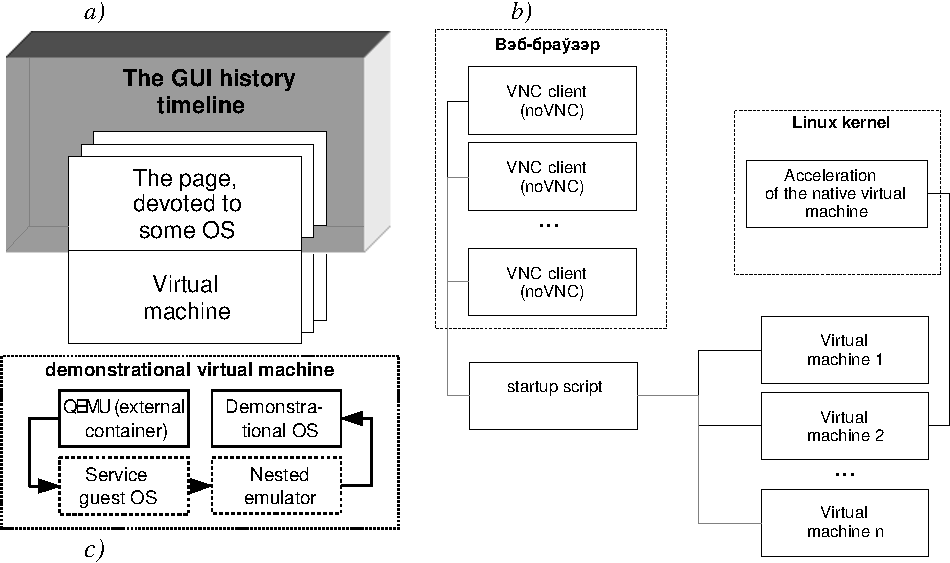
\includegraphics[scale=0.65]{100_2014_w-kostiuk1crop_en}
  \caption{Scheme of the document building (a), and components interaction (b) with nested virtualization (c)}
\end{figure}

The virtual machine is used as a fully isolated container storing a snapshot of the running OS \cite{kostiuk2}. Choice of QEMU is caused by the extremely simple transfer of virtual machine images between computers, and also by its ability to emulate not only x86"=compatible platforms, but also ones based on SPARC, PowerPC, Motorola 68k, MIPS and ARM processors, which are necessary to run many operating systems from 80s and 90s. However, currently multiplatformness of QEMU is poorly used, because the support of peripheral devices on alternative platforms at this emulator is rarely sufficient to boot ancient operating systems.

At the same time, there are emulators available to support virtually all ancient Intel"=incompatible systems "---community"=developed ones or created as the part of commercial SDK. The first variant is more common in desktop operating systems, so it was possible to enrich the timeline with Xerox Alto, Amiga, RiscOS, Apple Lisa, MacOS of 1.x, 7.x and X versions. Proprietary emulators for desktop operating systems are rare case and usually belong to the manufacturer of the OS, as in the case of Xerox GlobalView emulator. In case of mobile operating systems emulators from the SDK are dominating, such as Psion EPOC16 and EPOC32, PalmOS, Magic Cap, Windows CE, pre"=release versions of Android SDK. For now we use only one community"=developed mobile OS emulator "---Open Einstein project, which allows to run NewtonOS.

However, all these emulators don't support snapshots and the VNC protocol. Therefore a large part of demos is build along with the the nested virtualization scheme (see Fig. 1) where QEMU plays the role of an external container. 

Of course many operating systems do not require nested virtualiza\-tion and so internal emulator is not used for them. That's the case of desktop Windows OS oif 1.x, 2.x, 3.x and 95 versions, as far as IBM OS/2 2.x and 4.x, GEM from Digital Research, GEOS by Berkeley Softworks, as well as a number of mobile operating systems: Pen \linebreak Windows, Maemo, Android, WebOS (not least due to the fact that QEMU is often included in mobile SDK).

Freely distributable part of the timeline contains free/libre software systems (having such licenses from the very beginning, or opensourced because of the extreme aging or being a free clone of the abandoned commercial system). That's about different Unix"=based and Linux"=based desktop environments for desktop and mobile computers as well as GEM, Amiga, RiscOS, and HaikuOS.

The timeline material is still at the stage of filling; at this point the review has some missing objects, which have still played an important role in the history of graphical operating systems. Mainly these are new OS versions from Microsoft and Apple. In addition, DOS shell Visi On, and NeXTSTEP are incompatible with the current versions of QEMU. Currently we use Linux"=based GNUStep DE as the NeXTSTEP replacement. The problem with the Visi On can be solved using Bochs and VirtualBox, which is undesirable from the portability and resources consumption points of view.

The number of historically important GUI shells without runnable versions  appeared to be surprisingly small: currently this row includes multi"=window interface of Smalltalk from the late 70s, Xerox Star \linebreak Document Processor, as well as two mobile systems: PenPoint OS and IBM Simon. 

One more component can be seen in the scheme of embedded virtua\-lization "--- a service guest OS, which is used to start the nested emulator. Its choice is determined by the requirement of the minimum memory consumption, usage of idle CPU cycles, as well as support for USB bus emulation, which allows to emulate pointing devices in absolute coordinates. The latter requirement is important for a comfortable mouse control in a virtual machine \cite{kostiuk1}. As a service guest operating system in addition to multiple versions of Linux we have used FreeDOS and ReactOS. It should be further noted that ReactOS perfectly meets all three requirements, and thus in our own experience it is the first case of its successful application for some practical needs.


\begin{thebibliography}{9}
\bibitem{kostiuk1} Костюк Д.А. Особенности использования виртуализованных окружений, внедренных в презентационные материалы // Восьмая конференция «Cвободное программное обеспечение высшей школе»: тез. докл. / Переславль, 26--27 января 2012  года. М.: Альт Линукс, 2012. "---C. 83--86.
\bibitem{kostiuk2} Костюк Д.А., Дереченник С.С. Построение прозрачных виртуализованных окружений для изоляции уязвимых программных систем // Комплексная защита информации: матер. XVI научно-практич. конф., Гродно, 17--20 мая 2011 г. Гродно, 2011. "---С. 209--212. 
\end{thebibliography}
\end{document}

\documentclass[10pt, a5paper]{article}
\usepackage{pdfpages}
\usepackage{parallel}
\usepackage[T2A]{fontenc}
\usepackage{ucs}
\usepackage[utf8x]{inputenc}
\usepackage[polish,english,russian]{babel}
\usepackage{hyperref}
\usepackage{rotating}
\usepackage[inner=2cm,top=1.8cm,outer=2cm,bottom=2.3cm,nohead]{geometry}
\usepackage{listings}
\usepackage{graphicx}
\usepackage{wrapfig}
\usepackage{longtable}
\usepackage{indentfirst}
\usepackage{array}
\newcolumntype{P}[1]{>{\raggedright\arraybackslash}p{#1}}
\frenchspacing
\usepackage{fixltx2e} %text sub- and superscripts
\usepackage{icomma} % коскі ў матэматычным рэжыме
\PreloadUnicodePage{4}

\newcommand{\longpage}{\enlargethispage{\baselineskip}}
\newcommand{\shortpage}{\enlargethispage{-\baselineskip}}

\def\switchlang#1{\expandafter\csname switchlang#1\endcsname}
\def\switchlangbe{
\let\saverefname=\refname%
\def\refname{Літаратура}%
\def\figurename{Іл.}%
}
\def\switchlangen{
\let\saverefname=\refname%
\def\refname{References}%
\def\figurename{Fig.}%
}
\def\switchlangru{
\let\saverefname=\refname%
\let\savefigurename=\figurename%
\def\refname{Литература}%
\def\figurename{Рис.}%
}

\hyphenation{admi-ni-stra-tive}
\hyphenation{ex-pe-ri-ence}
\hyphenation{fle-xi-bi-li-ty}
\hyphenation{Py-thon}
\hyphenation{ma-the-ma-ti-cal}
\hyphenation{re-ported}
\hyphenation{imp-le-menta-tions}
\hyphenation{pro-vides}
\hyphenation{en-gi-neering}
\hyphenation{com-pa-ti-bi-li-ty}
\hyphenation{im-pos-sible}
\hyphenation{desk-top}
\hyphenation{elec-tro-nic}
\hyphenation{com-pa-ny}
\hyphenation{de-ve-lop-ment}
\hyphenation{de-ve-loping}
\hyphenation{de-ve-lop}
\hyphenation{da-ta-ba-se}
\hyphenation{plat-forms}
\hyphenation{or-ga-ni-za-tion}
\hyphenation{pro-gramming}
\hyphenation{in-stru-ments}
\hyphenation{Li-nux}
\hyphenation{sour-ce}
\hyphenation{en-vi-ron-ment}
\hyphenation{Te-le-pathy}
\hyphenation{Li-nux-ov-ka}
\hyphenation{Open-BSD}
\hyphenation{Free-BSD}
\hyphenation{men-ti-on-ed}
\hyphenation{app-li-ca-tion}

\def\progref!#1!{\texttt{#1}}
\renewcommand{\arraystretch}{2} %Іначай формулы ў матрыцы зліпаюцца з лініямі
\usepackage{array}

\def\interview #1 (#2), #3, #4, #5\par{

\section[#1, #3, #4]{#1 -- #3, #4}
\def\qname{LVEE}
\def\aname{#1}
\def\q ##1\par{{\noindent \bf \qname: ##1 }\par}
\def\a{{\noindent \bf \aname: } \def\qname{L}\def\aname{#2}}
}

\def\interview* #1 (#2), #3, #4, #5\par{

\section*{#1\\{\small\rm #3, #4. #5}}

\def\qname{LVEE}
\def\aname{#1}
\def\q ##1\par{{\noindent \bf \qname: ##1 }\par}
\def\a{{\noindent \bf \aname: } \def\qname{L}\def\aname{#2}}
}

\begin{document}
\def\v!#1!{\texttt{#1}}
\title{Удобства и особенности OpenBSD Ports}
\author{Vadim Zhukov, Moscow, Russia}
\maketitle
\begin{abstract}
OpenBSD acquired Ports framework from FreeBSD many years ago, and since then those frameworks diversed very much. Current OpenBSD Ports infrastructure makes it possible to have many up-to-date ports, including ‘heavy’ ones like GNOME, LibreOffice and KDE, by relatively few number active maintainers. This talk is about features of current OpenBSD ports system: bulk package builds, package signing and updating, manual library versions handling, modules framework and other stuff.
\end{abstract}
Как в любой нормальной современной ОС общего назначения, в OpenBSD есть механизм для установки стороннего ПО. В данном случае "--- OpenBSD Ports, происходящие, как многие знают, от FreeBSD Ports. Однако, сохранив ряд внешних признаков прародителя, OpenBSD Ports кардинально отличаются от FreeBSD Ports внутри. Проще всего это показать, перечислив то, что сохранилось:

\begin{enumerate}
  \item Использование Makefile для описания порта.
  \item Названия основных операций и ряд переменных, используемых в этом Makefile.
\end{enumerate}

Во всём остальном OpenBSD Ports заметно ушли вперёд "--- впрочем, разработчики FreeBSD раскачались и стали догонять, что видно на примере свежевышедшей FreeBSD 10.

Ключевые особенности OpenBSD Ports:

\begin{enumerate}
  \item Сборка пакета "--- обязательный этап. Пакет сначала собирается, и только потом ПО устанавливается из него в систему.
  \item Контроль сборки посредством \v!systrace!(1), \v!sudo!(8), fake"=фреймворка и \v!pkg\_create!(1). Файлы для пакета помещаются в отдельный каталог, а не прямо на рабочую систему. В ходе «фальшивой установки» отлавливается запись за пределы рабочего каталога (кроме /tmp и /var/tmp).
  \item Поддержание целостности дерева портов посредством непрерывной сборки пакетов с использованием dpb(1).
  \item Четыре вида зависимостей: \v!BUILD\_DEPENDS!, \v!LIB\_DE\-PENDS!, \v!RUN\_DEPENDS!, \v!TEST\_DEPENDS!.
  \item Опции и субпакеты, см. «FLAVORS AND MULTI\_PACKAGES» в \v!bsd.port.mk!(5).
  \item Модули, см. \v!port-modules!(7).
  \item Реально работающий механизм обновления пакетов, с учётом переименований, требований к конкретным версиям, наличия конфликтов и т.\,д.
  \item Ручной контроль версий «публичных» разделяемых библиотек.
\end{enumerate}

Благодаря имеющимся средствам автоматизации большинства рутинных операций и жёстком контролю в виде \v!dpb!(1), на поддержание высокого качества пакетов уходит сравнительно небольшое количество сил. Как результат, в OpenBSD при сравнительно небольшом количестве мейнтейнеров поддерживается большая часть современного софта. Текущие примеры:

\begin{itemize}
  \item порты GNOME и XDG-стек поддерживаются всего двумя \linebreak людьми
  \item порты LibreOffice и Chromium "--- одним и тем же человеком
  \item KDE 3 и 4 "--- одним и тем же человеком
  \item все порты Mozilla-приложений "--- одним и тем же человеком
\end{itemize}

О субпакетах и опциях:

OpenBSD Ports, как и другие аналогичные системы, позволяет задавать для пакетов опции сборки. Основные отличия OpenBSD в этой области следующие:

\begin{itemize}
  \item Количество опций OpenBSD старается поддерживать на минимальном уровне. Это позволяет при разумных усилиях тестировать все или почти все возможные варианты пакетов.
  \item Используемые при сборке опции записываются в имя пакета через дефис, после номера версии. Например:\\
\verb!kdelibs-4.11.5-debug!\\
\verb!vim-7.4.45p2-huge-gtk2-python!
\end{itemize}


Благодаря этому в репозитории пакетов вместе могут одновременно находиться разные варианты пакетов, и не возникает вопросов вроде «какие опции были использованы для пакета?».

Изначально в FreeBSD Ports было чёткое соответствие: одна сборка "--- один пакет. Когда требовалось собирать несколько разных пакетов на базе одного порта (например: \v!postgresql"=client! и \v!postgresql"=server!), то один порт включал себя директивой \v!.in\-clu\-de! другой, незначительно модифицировал переменные и предоставлял альтернативный plist. Таким образом, сборка этих двух пакетов должна была бы происходить дважды, либо требовала довольно «грязных» хаков.

В OpenBSD Ports имеется возможность создавать из одного порта несколько пакетов. Строго говоря, корректнее было бы говорить о субпортах, а не субпакетах, так как создаваемые пакеты являются изначально независимыми и могут иметь любые (допустимые) имена. Однако менять название переменной теперь никто не собирается.

Названия самих субпакетов начинаются с дефиса. Это делается для возможности отличать субпакеты от опций в \v!FULL\-PKG\-PATH! "--- своеобразном «пути», используемом для пакета с портом, из которого он собирается. \v!FULL\-PKG\-PATH! "--- своего рода идентификатор (суб-)пакета и играет большую роль на всех этапах работы с пакетами.

Наравне с \v!FULLPKGPATH! имеется \v!FULL\-PKG\-NAME!. Если \v!PKG\-NAME! содержит собственно название пакета и его версию, то в \v!FULL\-PKG\-NAME! к этому добавляются номера ревизии порта (\v!RE\-VI\-SI\-ON!) и эпохи порта (\v!EPOCH!), а также используемые опции. Именно \v!FULL\-PKG\-NAME! и становится именем конечного файла, содержащего собранный пакет (не считая расширения).

Для портов также можно задавать псевдоопции (\v!PSEUDO\_FLA\-VORS!). Они используются в тех случаях, когда необходимо управлять сборкой порта без влияния на содержимое создаваемых пакетов. Обычно это ситуации, когда нужно избежать лишних зависимостей при сборке, когда какие-то субпакеты являются лишними, или, например, зависимости нужны только для прогона тестов. Псевдоопции не записываются в имени пакета.

Так как отдельные субпакеты могут выпадать и по другим причинам (например, непригодность для какой-то аппаратной архитектуры) посредством переменных вида \v!BROKEN"=subpkg! и \v!IGNORE"=subpkg!, для конечного определения параметров сборки имеется \linebreak вспомогательный механизм \v!bsd.port.arch.mk!(5). Хотя внешне он кажется аналогом \v!bsd.port.pre.mk! из FreeBSD, назначение у них всё же разное: \v!bsd.port.arch.mk! используется только для двух вещей:
\begin{enumerate}
  \item Определение аппаратной архитектуры, под которую собирается пакет.
  \item Вычисление переменной \v!BUILD\_PA\-CKA\-GES!, содержащей список подлежащих сборке пакетов. После включения \linebreak \v!<bsd.port.arch.mk>! порт может использовать проверки вида \linebreak \texttt{.if \$\{BUILD\_PA\-CKA\-GES:M-subpkg\}} для определения, нужно ли включать сборку определённого субпакета.
\end{enumerate}

Результаты данных проверок обычно используются для установки специфичных параметров конфигурации и наборов зависимостей.

О модулях:

Модули "--- Makefile, подключаемые OpenBSD Ports по просьбе порта. Модули могут как модифицировать переменные, так и устанавливать или добавлять обработчики стандартных операций. Для подключения модуля достаточно добавить его имя в переменную \v!MODULES!. Примеры модулей:

\begin{enumerate}
  \item Один из самых простых модулей "--- \v!converters/libiconv!. Всё, что он делает "--- добавляет ряд зависимостей для порта и дополняет \v!WANTLIB! (список используемых портом разделяемых библиотек).
  \item Более сложный модуль "--- \v!devel/cmake!. Он используется портами, которые, как не трудно догадаться, собираются при помощи CMake. Данный модуль устанавливает ряд переменных, используемых CMake при конфигурировании и сборке, в том числе для: выбора движка сборки (поддерживаются make и Ninja), перекрытия версий разделяемых библиотек, настройки вывода прогресса сборки и т.\,д.
  \item Модуль \v!lang/ruby! "--- пожалуй, самый сложный в дереве портов; он даже получил персональную man-страницу: \linebreak\v!ruby"=module!(5). С его помощью собираются как обычные программы, зависящие от Ruby, так и Ruby gems, с платформо-зависимым кодом и без. Из возможностей модуля:
\end{enumerate}

\begin{itemize}
  \item Поддержка использования одним портом различных версий Ruby (включая JRuby и Rubinius) через механизм опций.
  \item Санация путей к интерпретатору Ruby в скриптах (замена \texttt{\#!/usr/bin/env} или \texttt{\#!/usr/bin/ruby} на то, с чем должен работать порт).
\end{itemize}

Функциональность, подобная описанной выше, присутствует и в других аналогичных модулях: \v!lang/python!, \v!lang/tcl!\ldots{}

О ручном контроле версий разделяемых библиотек:

Речь здесь пойдёт о самих библиотеках как объектах компиляции, а не о дистрибутивах ПО. Также следует сказать, что нижесказанное относится лишь к «публичным» библиотекам, которые используются при компиляции ПО. Всевозможные плагины и им подобные сущности не используются при компиляции, а загружаются динамически, посредством \v!dlopen()!, и располагаются в отдельных подкаталогах.

Для разделяемых библиотек существует соглашение о нумерации: \v!MAJOR.MINOR[.OTHER\ldots{}]!, со следующими правилами изменения версии:

\begin{itemize}
  \item Изменение в библиотеке, приводящее к изменению ABI без сохранения обратной совместимости: увеличение MAJOR.
  \item Изменение в библиотеке, не приводящее к изменению ABI, или же сохраняющее обратную совместимость ABI: увеличение MINOR.
\end{itemize}

Номер версии записывается в имени файла и/или в SONAME библиотеки. Когда требуется найти подходящую для программы версию библиотеки, поиск осуществляется с учётом вышеуказанного соглашения: MAJOR должна совпадать с тем, что требуется программе, а MINOR "--- быть не меньше требуемого программой. Казалось бы, всё довольно просто, но:

\begin{itemize}
  \item Часто разработчики смешивают версию дистрибутива, поставляющего библиотеку, с её внутренним номером. В результате, смена внутреннего номера библиотеки находится в полном отрыве от реальности.
  \item В других случаях не производится изменение внутреннего номера библиотеки, или изменяется не та часть номера. В результате, после обновления установленной версии библиотеки, использующее её ПО может оказаться неработоспособным.
  \item Наконец, иногда в самой операционной системе могут происходить изменения, влияющие на ABI. В случае OpenBSD, правда, обычно делается увеличение MAJOR для libc, что автоматически «разделяет» разные поколения пакетов.
\end{itemize}

В силу вышеперечисленных причин, в OpenBSD введена практика использования собственной нумерации разделяемых библиотек. Ответственность за соблюдение правил ABI в этом случае ложится на того, кто подготавливает порт или его обновление. Это может показаться большим усложнением, однако на самом деле для всех популярных систем сборки в OpenBSD имеется поддержка перекрытия версий библиотек. Внешне эти изменения сводятся к следующему: когда система сборки готовится слинковать конечную версию библиотеки libfoo, то проверяется наличие переменной окружения \v!LIBfoo\_VERSION! и, если такая установлена, использует её значение вместо заданного в конфигурации сборки разработчиком. Таким образом, максимум, что приходится делать при подготовке (обновления) порта "--- это второй раз его собрать, если были пропущены какие-то библиотеки; обычно инфраструктура портов сама обнаруживает и уведомляет о таковых при выполнении операции «\v!make update-plist!».

Версии разделяемых библиотек играют большую роль при обновлении ПО, так как позволяют осуществлять плавную миграцию между версиями использующего библиотеки ПО.

\end{document}

\documentclass[10pt, a5paper]{article}
\usepackage{pdfpages}
\usepackage{parallel}
\usepackage[T2A]{fontenc}
\usepackage{ucs}
\usepackage[utf8x]{inputenc}
\usepackage[polish,english,russian]{babel}
\usepackage{hyperref}
\usepackage{rotating}
\usepackage[inner=2cm,top=1.8cm,outer=2cm,bottom=2.3cm,nohead]{geometry}
\usepackage{listings}
\usepackage{graphicx}
\usepackage{wrapfig}
\usepackage{longtable}
\usepackage{indentfirst}
\usepackage{array}
\newcolumntype{P}[1]{>{\raggedright\arraybackslash}p{#1}}
\frenchspacing
\usepackage{fixltx2e} %text sub- and superscripts
\usepackage{icomma} % коскі ў матэматычным рэжыме
\PreloadUnicodePage{4}

\newcommand{\longpage}{\enlargethispage{\baselineskip}}
\newcommand{\shortpage}{\enlargethispage{-\baselineskip}}

\def\switchlang#1{\expandafter\csname switchlang#1\endcsname}
\def\switchlangbe{
\let\saverefname=\refname%
\def\refname{Літаратура}%
\def\figurename{Іл.}%
}
\def\switchlangen{
\let\saverefname=\refname%
\def\refname{References}%
\def\figurename{Fig.}%
}
\def\switchlangru{
\let\saverefname=\refname%
\let\savefigurename=\figurename%
\def\refname{Литература}%
\def\figurename{Рис.}%
}

\hyphenation{admi-ni-stra-tive}
\hyphenation{ex-pe-ri-ence}
\hyphenation{fle-xi-bi-li-ty}
\hyphenation{Py-thon}
\hyphenation{ma-the-ma-ti-cal}
\hyphenation{re-ported}
\hyphenation{imp-le-menta-tions}
\hyphenation{pro-vides}
\hyphenation{en-gi-neering}
\hyphenation{com-pa-ti-bi-li-ty}
\hyphenation{im-pos-sible}
\hyphenation{desk-top}
\hyphenation{elec-tro-nic}
\hyphenation{com-pa-ny}
\hyphenation{de-ve-lop-ment}
\hyphenation{de-ve-loping}
\hyphenation{de-ve-lop}
\hyphenation{da-ta-ba-se}
\hyphenation{plat-forms}
\hyphenation{or-ga-ni-za-tion}
\hyphenation{pro-gramming}
\hyphenation{in-stru-ments}
\hyphenation{Li-nux}
\hyphenation{sour-ce}
\hyphenation{en-vi-ron-ment}
\hyphenation{Te-le-pathy}
\hyphenation{Li-nux-ov-ka}
\hyphenation{Open-BSD}
\hyphenation{Free-BSD}
\hyphenation{men-ti-on-ed}
\hyphenation{app-li-ca-tion}

\def\progref!#1!{\texttt{#1}}
\renewcommand{\arraystretch}{2} %Іначай формулы ў матрыцы зліпаюцца з лініямі
\usepackage{array}

\def\interview #1 (#2), #3, #4, #5\par{

\section[#1, #3, #4]{#1 -- #3, #4}
\def\qname{LVEE}
\def\aname{#1}
\def\q ##1\par{{\noindent \bf \qname: ##1 }\par}
\def\a{{\noindent \bf \aname: } \def\qname{L}\def\aname{#2}}
}

\def\interview* #1 (#2), #3, #4, #5\par{

\section*{#1\\{\small\rm #3, #4. #5}}

\def\qname{LVEE}
\def\aname{#1}
\def\q ##1\par{{\noindent \bf \qname: ##1 }\par}
\def\a{{\noindent \bf \aname: } \def\qname{L}\def\aname{#2}}
}

\begin{document}
\title{Операционная система Linux как основа для построения высокопроизводительных систем хранения данных}
\author{Александр Фахрутдинов, Сызрань, Russia}
\maketitle
\begin{abstract}
Report describes some Linux kernel subsystems which can be used to create a high-performance data storage. Well-known instruments of storage management (RAID and LVM) are explained as far as cutting-edge technologies for multi-level caching and data tiering. Also, kernel-mode virtual target device  for remote access to data storage from other hosts is reviewed.
\end{abstract}
Системы хранения данных (СХД) "--- это одна из основ современного мира компьютерных технологий. С возникновением облачных сред и повсеместном внедрением виртуализации возникла необходимость в сверхскоростных хранилищах большого объема и повышенной  отказоустойчивости. Кроме того, потребовались «умные» системы, которые хранят вместо несколько копий одних и тех же данных только одну, выделяют под данные именно столько реально имеющегося дискового пространства, сколько требуется, а не сколько запросит пользователь, умеют копировать массивы данных внутри устройства без отправки их на сервер и так далее.

Для организации эффективного хранения данных в Linux применяются виртуальные блочные устройства, которые представляют собой прослойку между собственно аппаратным хранилищем данных, например, жестким диском, и приложениями. Классический случай применения таких устройств программные дисковые массивы "--- RAID. За   обслуживание  RAID в Linux отвечает подсистема md (multiplie devices), которая позволяет создавать основные типы RAID "--- простое объединение дисков (JBOD), RAID уровней 0, 1 (зеркало), 4, 5, 6, а также "--- RAID 10.
.
RAID обеспечивает объединение дисков и отказоустойчивость в пределах одного сервера, однако он не решет проблему распределения пространства массива. Для управления дисковым пространством в Linux принято использовать менеджер виртуальных томов "--- LVM. Он позволяет гибко распределять место на дисках между приложениями, поддерживает создание, удаление и изменение размера тома «на лету», а также позволяет создавать собственные массивы типа JBOD,  RAID 0 и 1. Кроме того, LVM обеспечивает создание мгновенных снимков (snapshot) томов вне зависимости от того, поддерживает ли снимки файловая система тома, причем снимки доступны не только на чтение, но и на запись.  Однако платой за эту универсальность является низкое быстродействие снимков, что ограничивает область их применения.

В основе md и LVM лежит система проецирования устройств "--- device-mapper (dm). Она предоставляет единый механизм для создания на базе простых блочных устройств более сложных, наделенных дополнительными функциями. Возможности dm расширяются при помощи модулей, называемых «mapping targets». В стандартном ядре Linux, кроме md и LVM, присутствуют модули общего назначения для следующих целей:

\begin{itemize}
  \item диагностика и тестирование\begin{itemize}
  \item создание фиксированной задержки "--- dm-delay
  \item имитация сбоев "--- dm-flakey
  \item сбор статистики об обращениях к конкретным областям устройства "--- dm-statistics
  \item имитация пустого устройства "--- dm-zero
  \item проверка цифровой подписи тома "--- dm-verity
\end{itemize}


  \item построение RAID 0, 1 "--- dm-mod
  \item шифрование тома "--- dm-crypt
  \item доступ к подсистеме md для управления массивами через интерфейс device-mapper "--- dm-raid
\end{itemize}

Кроме того, в состав ядра входят модули, применяемые в высокопроизводительных СХД уровня предприятия

\begin{itemize}
  \item доступ к хранилищу через множество путей\begin{itemize}
  \item с простым резервированием "--- dm-multipath
  \item с учетом длины очереди "--- dm-queue-length
  \item с учетом времени доступа "--- dm-service-time
  \item доступ к разным регионам хранилища через разные пути "--- dm-switch
\end{itemize}


  \item кэширование данных на твердотельных накопителях\begin{itemize}
  \item dm-cache (с версии ядра 3.9,  релиз 28 апреля 2013)
  \item bcache (с версии 3.10, релиз 30 июня 2013)
  \item flashcache (разработка Facebook, не включен в ядро)
\end{itemize}


  \item не включены в ядро, но могут быть полезны:\begin{itemize}
  \item «многослойное» хранилище из разных типов дисков "--- btier
  \item RAM-диск с периодическим сохранением информации "--- eprd
Как известно, в Linux кэшируется только доступ к файловой системе, доступ же напрямую к блочным устройствам не кэшируется, поэтому одним из способов повысить быстродействие, особенно в может быть применение указанных выше модулей. В особенности это справедливо для систем виртуализации.
\end{itemize}


\end{itemize}

В системах  виртуализации принято выделять дисковое пространство не на этапе создания виртуальной машины, а по мере необходимости (thin provisioning). Device mapper имеет подобный функционал, начиная с ядра 3.2 (релиз 4 января 2012). Модуль dm-thin-pool позволяет создавать виртуальные устройства, которые не резервируют весь предназначенный им объем в момент создания, а расходуют выделенное физическое пространство по мере заполнения самого устройства данными. Также dm-thin-pool поддерживает возврат более не используемых блоков в общий пул, если вышележащая файловая система уведомит его об этом. Кроме того, модуль dm-thin-pool  позволяет создавать виртуальное устройство на базе шаблона, в роли которого выступает другое устройство, доступное только для чтения.

Несмотря на то, что device-mapper обладает широким функционалом, нельзя не заметить, что его назначение "--- создание виртуальных устройств «высокого уровня», которые служат для управления уже имеющимся дисковым пространством и должны опираться на программный или аппаратный RAID. В то же время  device-mapper не обеспечивает доступ к созданному устройству за пределами хоста, например, по протоколам iSCSI и FC. Для этих целей в ядро Linux не так давно была включена инфраструктура LIO-target.

LIO-target "--- это разработка компании Rising Tide Systems, которая была лицензирована под  GPL и включена в ядро Linux, начиная с версии 2.6.38 (релиз 15 января 2011 г.). В 2013 году разработчики LIO-target покинули  Rising Tide Systems и основали компанию Datera, целью которой является разработка программного обеспечения для СХД.

LIO-target состоит из высокоскоростного виртуального блочного устройства с поддержкой расширенного набора команд SCSI, драйверов нижнего уровня (бэкэндов), при помощи которых виртуальное устройство отображается на реальное и драйверов верхнего уровня (фронтэндов), при помощи которых можно получить доступ к устройству из-за пределов хоста.
Поддерживаются следующие бэкэнды:

\begin{itemize}
  \item FILEIO "--- обращение к нижележащему блочному устройству как к файлу через слой виртуальной ФС.
  \item BLOCKIO "--- обращение к нижележащему блочному устройству при помощи команд SCSI.
  \item PSCSI "--- пересылка команд  SCSI физическому   устройству, например, RAID-контроллеру, без обработки.
  \item Memory Copy RAMDISK "--- блочное устройство в оперативной памяти.
Фронтэнды обеспечивают подключение к LIO-target других хостов. В настоящий момент поддерживаются интерфейсы iSCSI, FCoE, Fibre Channel, InfiniBand, IBM vSCSI, FireWare и USB. Кроме того, возможна эмуляция блочного устройства на локальной машине, а также передача такого устройства внутрь виртуальной машины под управлением \linebreak KVM (vHost).
\end{itemize}

Особенностью  LIO-target является поддержка SCSI-команд аппаратного ускорения для систем хранения данных (VAAI). Эти команды используются, в первую очередь, системами виртуализации и призваны разгрузить гипервизор при таких ресурсоемких операциях, как клонирование виртуальной машины. До недавнего времени этот набор команд был реализован только в коммерческих СХД, теперь же он доступен всем пользователям ОС Linux.

Таким образом, ОС Linux предоставляет функционал, достаточный для построения на базе конкретной аппаратной платформы надежного и высокопроизводительного хранилища, которое может быть использовано как само по себе, так и в качестве узла в распределенной системе хранения данных.

\end{document}

\documentclass[10pt, a5paper]{article}
\usepackage{pdfpages}
\usepackage{parallel}
\usepackage[T2A]{fontenc}
\usepackage{ucs}
\usepackage[utf8x]{inputenc}
\usepackage[polish,english,russian]{babel}
\usepackage{hyperref}
\usepackage{rotating}
\usepackage[inner=2cm,top=1.8cm,outer=2cm,bottom=2.3cm,nohead]{geometry}
\usepackage{listings}
\usepackage{graphicx}
\usepackage{wrapfig}
\usepackage{longtable}
\usepackage{indentfirst}
\usepackage{array}
\newcolumntype{P}[1]{>{\raggedright\arraybackslash}p{#1}}
\frenchspacing
\usepackage{fixltx2e} %text sub- and superscripts
\usepackage{icomma} % коскі ў матэматычным рэжыме
\PreloadUnicodePage{4}

\newcommand{\longpage}{\enlargethispage{\baselineskip}}
\newcommand{\shortpage}{\enlargethispage{-\baselineskip}}

\def\switchlang#1{\expandafter\csname switchlang#1\endcsname}
\def\switchlangbe{
\let\saverefname=\refname%
\def\refname{Літаратура}%
\def\figurename{Іл.}%
}
\def\switchlangen{
\let\saverefname=\refname%
\def\refname{References}%
\def\figurename{Fig.}%
}
\def\switchlangru{
\let\saverefname=\refname%
\let\savefigurename=\figurename%
\def\refname{Литература}%
\def\figurename{Рис.}%
}

\hyphenation{admi-ni-stra-tive}
\hyphenation{ex-pe-ri-ence}
\hyphenation{fle-xi-bi-li-ty}
\hyphenation{Py-thon}
\hyphenation{ma-the-ma-ti-cal}
\hyphenation{re-ported}
\hyphenation{imp-le-menta-tions}
\hyphenation{pro-vides}
\hyphenation{en-gi-neering}
\hyphenation{com-pa-ti-bi-li-ty}
\hyphenation{im-pos-sible}
\hyphenation{desk-top}
\hyphenation{elec-tro-nic}
\hyphenation{com-pa-ny}
\hyphenation{de-ve-lop-ment}
\hyphenation{de-ve-loping}
\hyphenation{de-ve-lop}
\hyphenation{da-ta-ba-se}
\hyphenation{plat-forms}
\hyphenation{or-ga-ni-za-tion}
\hyphenation{pro-gramming}
\hyphenation{in-stru-ments}
\hyphenation{Li-nux}
\hyphenation{sour-ce}
\hyphenation{en-vi-ron-ment}
\hyphenation{Te-le-pathy}
\hyphenation{Li-nux-ov-ka}
\hyphenation{Open-BSD}
\hyphenation{Free-BSD}
\hyphenation{men-ti-on-ed}
\hyphenation{app-li-ca-tion}

\def\progref!#1!{\texttt{#1}}
\renewcommand{\arraystretch}{2} %Іначай формулы ў матрыцы зліпаюцца з лініямі
\usepackage{array}

\def\interview #1 (#2), #3, #4, #5\par{

\section[#1, #3, #4]{#1 -- #3, #4}
\def\qname{LVEE}
\def\aname{#1}
\def\q ##1\par{{\noindent \bf \qname: ##1 }\par}
\def\a{{\noindent \bf \aname: } \def\qname{L}\def\aname{#2}}
}

\def\interview* #1 (#2), #3, #4, #5\par{

\section*{#1\\{\small\rm #3, #4. #5}}

\def\qname{LVEE}
\def\aname{#1}
\def\q ##1\par{{\noindent \bf \qname: ##1 }\par}
\def\a{{\noindent \bf \aname: } \def\qname{L}\def\aname{#2}}
}

\begin{document}
\title{Steganography "--- coding and intercepting the information from encoded pictures in the absence of any initial information}
\author{Monika Kwiatkowska, Lublin, Poland \\ \L{}ukasz \'S{}wierczewski, \L{}om\.z{}a, Poland}
\maketitle
\begin{abstract}
The work includes implementation and extraction algorithms capabilities test, without any additional data (starting position, the number of bits used, gap between the amount of data encoded) information from encoded files (mostly images). The software is written using OpenMP standard which allowed them to run on parallel computers. Performance tests were carried out on computers, Blue Gene/P, Blue Gene/Q and the system consisting of four AMD Opteron 6272. Source code is available under GNU GPL v3 license and are available in a repository OLib.
\end{abstract}
\section{Introduction}

Steganography is the science of determining how to conduct commu\-ni\-ca\-tion so that the presence of the message could not be detected by third parties. It differs from cryptography in a way that in cryptography existence of the message is not negated but its content remains implicit. Steganography hides the fact that any communication has been con\-duct\-ed.

Differences between steganography and cryptography is shown in Table 1.

\section{Traditional Steganography}
The use of steganography dates back to the time of Herodotus, the fifth century BC. Examples of traditional steganography can be tattooing the scalp (after the hair grew back information remains in\-vi\-sible). One of the best solutions of this kind applied by the Germans during World War II "--- microdots technique. It was based on minimazing  pictures to such scale so that you can paste them into the text as a dot.

\begin{table}[t!]
\begin{center}
\begin{tabular}{P{13em}|c|c}
\hline
                                                                            & Cryptography & Steganography \\
\hline
Transforming information into a form in\-compre\-hensible by third parties  &     Yes      &     Yes       \\
Hiding information                                                          &     No       &     Yes       \\
Key usage                                                                   &     Yes      &     Yes       \\
Hiding the fact of commu\-ni\-ca\-tion                                      &     No       &     Yes       \\
Ensuring anonymity of commu\-ni\-ca\-ting parties                           &     No       &     Yes       \\
The amount of information transmitted to the encrypted information          &  Comparable  &  Much greater \\
\hline
\end{tabular}

Table 1. Differences between steganography and cryptography.
\end{center}
\end{table}

\section{Digital Steganography}

With the development of digital technology, steganography has found a new use also in the field of science. Digital steganography bases on making subtle changes to the original medium, and therefore gives a much more possibilities than traditional steganography.

The carrier of concealed information can be virtually any file (one that can be modified without having to worry about damage to its internal structures). However, the most commonly used are multimedia files "--- these are relatively large in size and difficult to capture the modification of original file.

Digital steganography depending on the type of operation can be divided into the following categories:

\begin{itemize}
  \item Substitutional
  \item Transformational
  \item Spectrum modification
  \item Spectrum spread
  \item Distortional
  \item Statistical
  \item Carrier generation
\end{itemize}

Another field of use for steganography is to communicate using VoIP technology. The Polish jargon adopted using in this case the word ‘steganphony’. The first such solution had been proposed by two Polish scientists Wojciech Mazurczyk and Krzysztof Szczypiorski in 2008 at a conference in Mexico \footnotemark[11]. It was based on in transferring the hidden content in the delayed packets, which according to a standard communication protocol (operating in real time) are omitted.

\section{LSB "--- Least Significant Bit "--- one of the methods of substitution}

The article will summarize often used method of substitution "--- LSB. Mostly it uses the least significant bits to record information. These bits often carry only noise and are insignificant from the point of view images for example. The principle of LSB operation for one and two least significant bits are shown in Figure 1 and Figure 2.

\begin{figure}[h!]
  \centering
  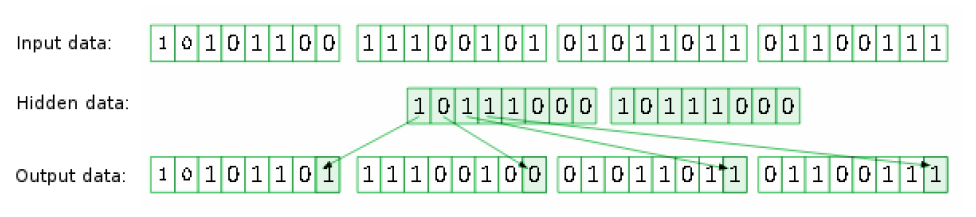
\includegraphics[width=\textwidth]{103_2014_w_Kwiatkowska_lsb1.png}
  Figure 1. Applying the LSB using one least significant bit.
\end{figure}

\begin{figure}[h!]
  \centering
  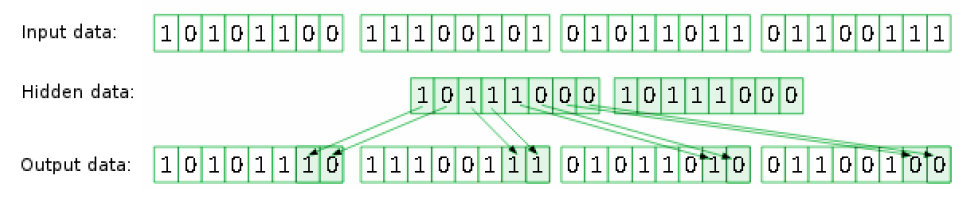
\includegraphics[width=\textwidth]{103_2014_w_Kwiatkowska_lsb2.png}
  Figure 2. Application of the LSB method using the two least significant bits.
\end{figure}

\section{Implementation}

Source code had been implemented in pure ANSI C. Sample code for function encrypting text using least significant bits of the image you can see in Listing 1.

\begin{verbatim}
int crypt_space_1bit(char * buffer, char *open_text,
  long int start_position, long int open_text_size,
  long int space_size)
{
  long int i;
  for (i = 0; i < (open_text_size * 8); i++)
  {
    if (check_bit(open_text[i / 8], i % 8))
    {
      set_bit(buffer[start_position + i * space_size], 0);
    }
    else
    {
      clear_bit(buffer[start_position + i * space_size], 0);
    }
  }
}
\end{verbatim}
Listing 1. The function encrypting the data in the image using one least significant bit.\\~

We are passing pointers to two array to the function "--- the buffer array (image data) and open\_text array (array of information to be encoded). In addition, the code uses macros check\_bit, set\_bit and clear\_bit. Their definition is shown in Listing 2.

\begin{verbatim}
# define check_bit(var,pos) ((var) & (1LL<<(pos)))
# define set_bit(var,pos) ((var) |= (1LL<<(pos)))
# define clear_bit(var,pos) ((var) &= ~{}(1LL<<(pos)))
\end{verbatim}
Listing 2. Macros defining operations on bits.\\~

The most important, in the case of this article, however, is a function used to extract encrypted text without knowledge of the initial starting value, or even the length of ciphertext. It has been shown in Listing 3.

\begin{verbatim}
long int breaker_standard_1bit_unknown_size_openmp(
  char *buffer, long int buffer_size, long int size_down,
  long int size_upper, result_structure *result,
  int number_of_threads)
{
  char *open_text;
  long int start_position;
  long int index_result;
  index_result = 0;
  long int i;
  long int j;
  j = size_down;

  #pragma omp parallel for shared(buffer, buffer_size, \
      size_down, size_upper, result, index_result)     \
      private(i, j, start_position, open_text)         \
      num_threads(number_of_threads)
  for(i=0; i < (buffer_size - j); i++)
  {
    open_text = (char *)malloc((size_upper + 1) * sizeof(char));
    start_position = i;
    for (j = size_down; j <= size_upper; j++)
    {
      encrypt_standard_1bit(buffer, open_text, start_position, j);
      if (ascii_veryfi(open_text, j) == 1)
      {
        open_text[j] = '\0';
        #pragma omp critical
        {
          result[index_result].start_position = i;
          strcpy(result[index_result].text, open_text);
          index_result++;
        }
      }
    }
    free(open_text);
  }
  return index_result;
}
\end{verbatim}
Listing 3. Function to extract information from the least significant bits without the initial information.\\~

This function searches the least significant bits in the buffer array of size of buffer\_size and searches all the possible encrypted patterns of lengths from size\_down to size\_upper. The result is inserted into the result array. The code uses so"=called pragma derived from the OpenMP standard. This pragma aims to parallelize the main loop. Also worth mentioning is separate critical section "--- it takes care of the correct addition of blocks to the results array. Only one thread can access the critical section at a time. Also a function has been used:

\verb!int ascii_verify(pointer, size);!

which verifies whether the starting substring at the pointer of length size is the correct text stored using ASCII code.

\section{Results}

Performance results obtained when searching for encoded text inside graphic file with a resolution of $1600\times1200$ is shown in Table 2. A similar table for resolution $4096\times4096$ is presented in Table 3. Additionally, obtained through parallel programming (OpenMP), speedup on IBM Blue Gene/Q and AMD Opteron 6272 is shown in Figure 3.


\begin{figure}[h!]
  \centering
  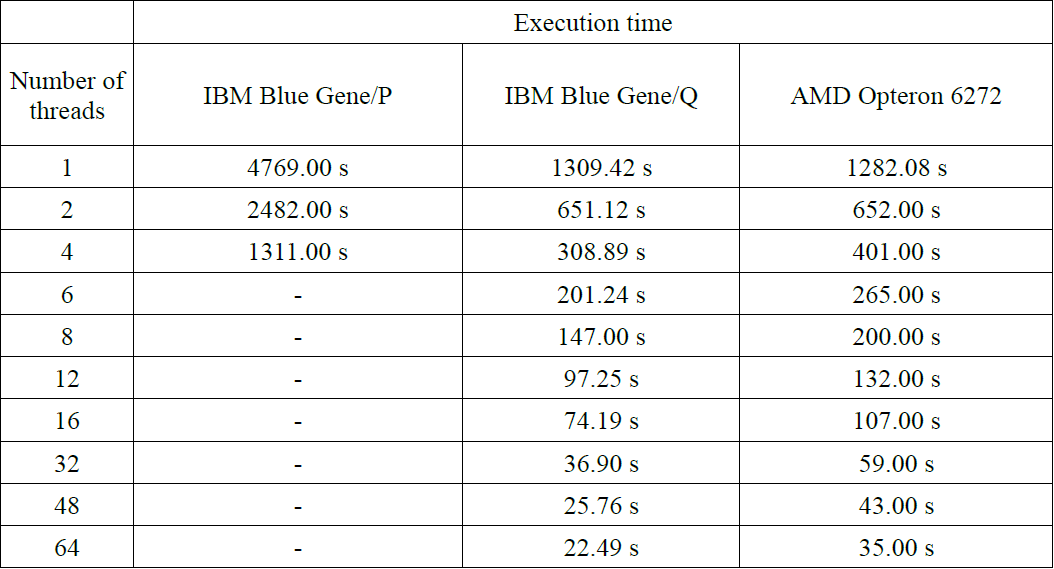
\includegraphics[width=\textwidth]{103_2014_w_Kwiatkowska_time2.png}
  Table 2. Performance results obtained during scan of the image with a resolution of $1600\times1200$ (searching one least significant bit using length of the search phrase in the range of 10 to 25).
\end{figure}

\begin{figure}[h!]
  \centering
  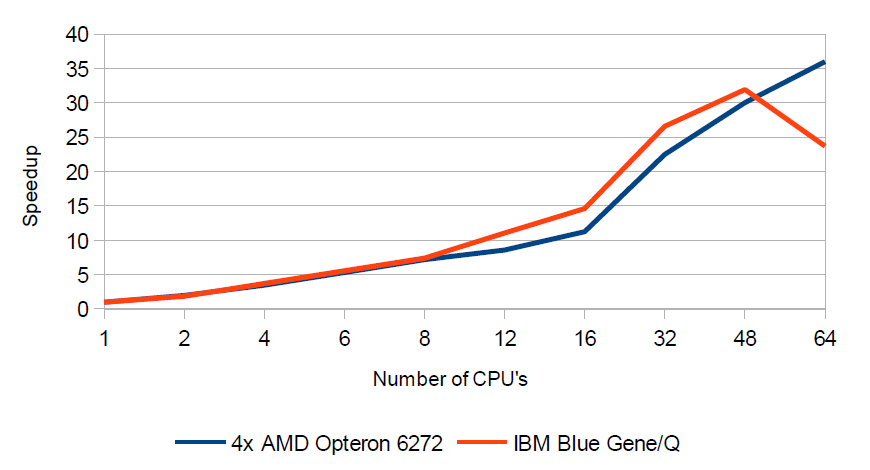
\includegraphics[width=\textwidth]{103_2014_w_Kwiatkowska_speedup.png}
  Figure 3. The speedup obtained on platforms AMD Opteron 6272 and IBM Blue Gene/Q while searching an image with a resolution of $1600\times1200$ (search only one least significant bit of the length of the text to search in the range from 10 to 25).
\end{figure}
\begin{figure}[h!]
  \centering
  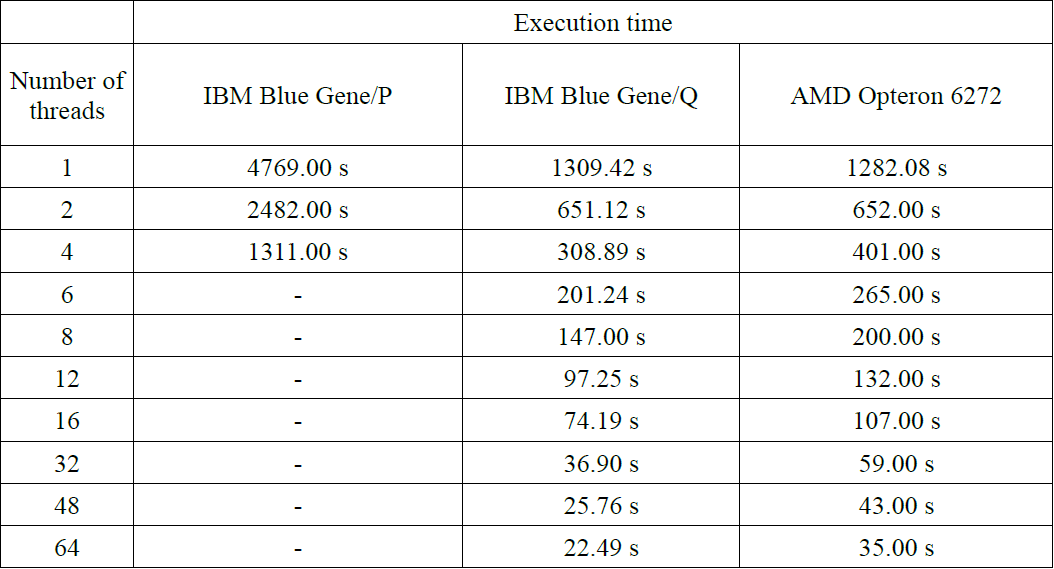
\includegraphics[width=\textwidth]{103_2014_w_Kwiatkowska_time2.png}
  Table 3. Performance results obtained during scan of the image with a resolution of $4096\times4096$ (searching one least significant bit using length of the search phrase in the range of 10 to 25).
\end{figure}

In the case of a platform consisting of four AMD Opteron 6272 maximum speedup is achieved by using 64 CPU and it reached 36.00. Using computational units used in Blue Gene/Q the speedup reached to 31.915. But it was not obtained, as might be expected, with a maximum (64) number of processors, but only 48. This may be due to the fact that one Blue Gene/Q CPU has only 16 physical cores that implement the execution of 64 threads.
It can also be noted that increasing the resolution of the analyzed image from $1600\times1200$ to $4096\times4096$ did not increase the runtime of the algorithm even tenfold "--- for applications executed sequentially on the Blue Gene/Q time increased from 193.11 seconds to 1309.42 seconds (about 6.78 times) and for the Blue Gene/P changed from 560.47 seconds to 4769.00 (about 8.50 times). Analysis has been performed for the speedup depending on the size of the hidden string searched. The results are shown in Table 3 (for AMD Opteron 6272) and in Table 4 (for Blue Gene/Q). Presentation of speedup obtained is presented in Figure 4. Additionally, Figure 5 shows the difference in the runtime of the sequential program execution between two platforms (AMD Opteron 6272 "--- IBM Blue Gene/Q).

\begin{figure}[h!]
  \centering
  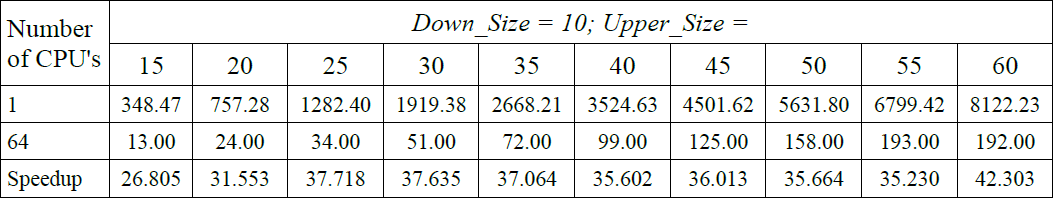
\includegraphics[width=\textwidth]{103_2014_w_Kwiatkowska_perf1.png}
  Table 4. The results of the analysis of performance for different sizes of searched hidden string [Down\_Size; Upper\_Size] (the ranges of [10, 15] to [10,60]) and platform based on AMD Opteron 6272.
\end{figure}
\begin{figure}[h!]
  \centering
  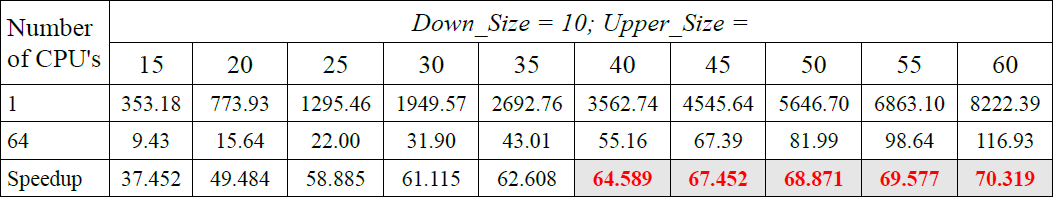
\includegraphics[width=\textwidth]{103_2014_w_Kwiatkowska_perf2.png}
  Table 5. The results of the analysis of performance for different sizes of searched hidden string [Down\_Size; Upper\_Size] (the ranges of [10, 15] to [10,60]) and platform based on processors installed in the Blue Gene/Q.
\end{figure}

\begin{figure}[h!]
  \centering
  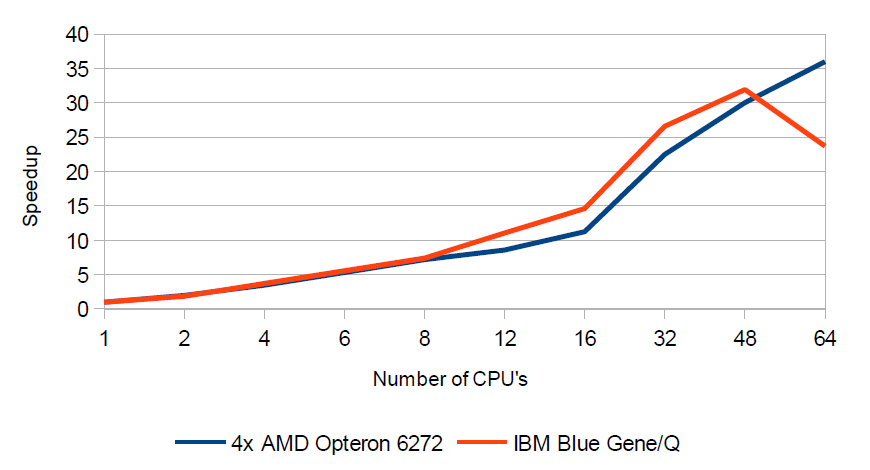
\includegraphics[width=\textwidth]{103_2014_w_Kwiatkowska_speedup.png}
  Figure 4. Graph showing the resulting speedup on AMD Opteron 6272 and IBM Blue Gene/Q in the analysis of performance for different sizes of searched hidden string.
\end{figure}

\begin{figure}[h!]
  \centering
  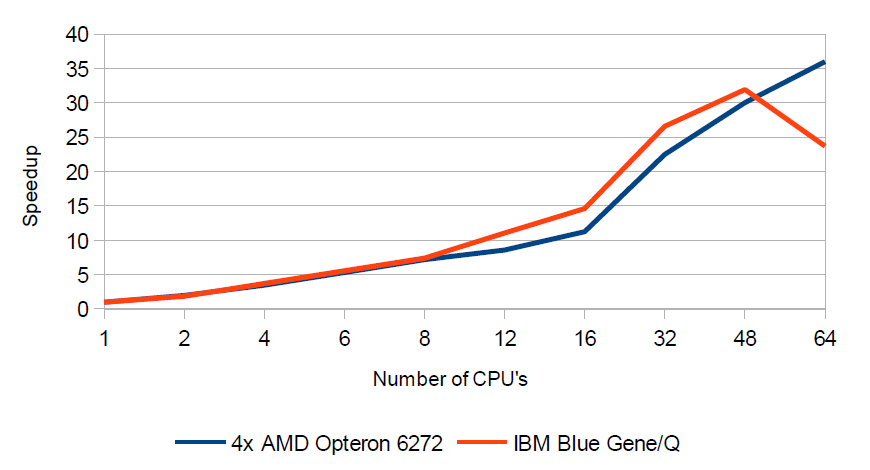
\includegraphics[width=\textwidth]{103_2014_w_Kwiatkowska_speedup.png}
  Figure 5. Graph showing the time difference obtained on a platform consisting of the AMD Opteron 6272 and obtained on the Blue Gene/Q in the analysis of performance for different sizes of searched hidden string.
\end{figure}

The strangest fact can be seen in the analysis of speedup presented in Table 5. According to the measurements on 64 processors for searching string of a length of 10 to 60 characters, maximum achieved speedup of 70.319, which is impossible and must be the result of the time measurment error. Problematic data in the table indicated in red. This anomaly is no longer present on the computer with four AMD Opteron 6272. However, in this case, the maximum speedup was only 42.303 and was obtained while searching a string with the length in the range [10, 60].

While in terms of speedup, the platform for the Blue Gene/Q is better but the lower sequential execution runtime of the program is always achieved on a computational node with AMD Opteron 6272 "--- it is confirmed in Figure 5. Differences in the runtime between these two systems, however, are relatively small and do not exceed 2\%.

\section{Conclusions and capabilities of work development}

Using the abilities of parallel programming, one  can very effectively deal with data processing in the field of steganography. LSB technique is used in most commercial software.

The work can be treated as a base for discussion, because it is very difficult to find a practical application of implemented steganography methods in the modern world. In the so-called ‘pure steganography’ strenght of encryption is mainly based on lack of knowledge about the techniques used by the individual encrypting the information \footnotemark[7]. So you can not publish this type of algorithms as Open Source. Such an approach, however, does not meet Kerckhoffs principle \footnotemark[10] stating, that a cryptographic system should be secured even if all the details about how it works (except the key) are known, and it is not recommended.

The presented work results concern the simplest variant in which the string is interpreted as ASCII code. Of course you can come up with your own, much more complicated system for the representation of characters.

\begin{figure}[h!]
  \centering
    
\includegraphics{103_2014_w_Kwiatkowska_lvee.png}\\
Figure 6. Logo of the LVEE conference with hidden text ‘LVEE – the best conference’.
\end{figure}

\section*{Acknowledgment}

Interdisciplinary Centre for Mathematical and Computational Modeling (ICM), Warsaw University, Poland is acknowledged for providing the computer facilities under the Grant No. G55-11.

\section*{Note}

The thesis presented on Winter LVEE 2014 Conference in Minsk (Belarus).

\section*{References}

\begin{enumerate}
  \item Dagum, Leonardo, and Ramesh Menon. ``OpenMP: an industry standard API for shared-memory programming.'' Computational Science \& Engineering, IEEE 5.1 (1998): 46-55.
  \item Lin, Heshan, et al. ``Massively parallel genomic sequence search on the Blue Gene/P architecture.'' High Performance Computing, Networking, Storage and Analysis, 2008. SC 2008. International Conference for. IEEE, 2008.
  \item Haring, Ruud A., et al. ``The IBM Blue Gene/Q compute chip.'' Micro, IEEE 32.2 (2012): 48-60.
  \item Keltcher, Chetana N., et al. ``The AMD Opteron processor for multiprocessor servers.'' Micro, IEEE 23.2 (2003): 66-76.
  \item OLib Library; http://lib.oproject.info
  \item Katzenbeisser S.: Information Hiding Techniques for Steganography and Digital Watermarking, s. 65 -- 105, 1999, Artech House
  \item Katzenbeisser S.: Information Hiding Techniques for Steganography and Digital Watermarking, s. 20 -- 23, 1999, Artech House
  \item Katzenbeisser, Stefan, and Fabien AP Petitcolas. Information hiding techniques for steganography and digital watermarking. Vol. 316. Norwood: Artech house, 2000.
  \item Kozieł, G. ``Przezroczystość danych ukrytych w sygnale audio.'' Pomiary, Automatyka, Kontrola 58 (2012): 972-974.
  \item Auguste Kerckhoffs, ``La cryptographie militaire'' Journal des sciences militaires, vol. IX, pp. 5–83, January 1883, pp. 161–191, February 1883.
  \item Mazurczyk, Wojciech, and Krzysztof Szczypiorski. ``Steganography of VoIP streams.'' On the Move to Meaningful Internet Systems: OTM 2008. Springer Berlin Heidelberg, 2008. 1001-1018.
\end{enumerate}

\end{document}

\documentclass[10pt, a5paper]{article}
\usepackage{pdfpages}
\usepackage{parallel}
\usepackage[T2A]{fontenc}
\usepackage{ucs}
\usepackage[utf8x]{inputenc}
\usepackage[polish,english,russian]{babel}
\usepackage{hyperref}
\usepackage{rotating}
\usepackage[inner=2cm,top=1.8cm,outer=2cm,bottom=2.3cm,nohead]{geometry}
\usepackage{listings}
\usepackage{graphicx}
\usepackage{wrapfig}
\usepackage{longtable}
\usepackage{indentfirst}
\usepackage{array}
\newcolumntype{P}[1]{>{\raggedright\arraybackslash}p{#1}}
\frenchspacing
\usepackage{fixltx2e} %text sub- and superscripts
\usepackage{icomma} % коскі ў матэматычным рэжыме
\PreloadUnicodePage{4}

\newcommand{\longpage}{\enlargethispage{\baselineskip}}
\newcommand{\shortpage}{\enlargethispage{-\baselineskip}}

\def\switchlang#1{\expandafter\csname switchlang#1\endcsname}
\def\switchlangbe{
\let\saverefname=\refname%
\def\refname{Літаратура}%
\def\figurename{Іл.}%
}
\def\switchlangen{
\let\saverefname=\refname%
\def\refname{References}%
\def\figurename{Fig.}%
}
\def\switchlangru{
\let\saverefname=\refname%
\let\savefigurename=\figurename%
\def\refname{Литература}%
\def\figurename{Рис.}%
}

\hyphenation{admi-ni-stra-tive}
\hyphenation{ex-pe-ri-ence}
\hyphenation{fle-xi-bi-li-ty}
\hyphenation{Py-thon}
\hyphenation{ma-the-ma-ti-cal}
\hyphenation{re-ported}
\hyphenation{imp-le-menta-tions}
\hyphenation{pro-vides}
\hyphenation{en-gi-neering}
\hyphenation{com-pa-ti-bi-li-ty}
\hyphenation{im-pos-sible}
\hyphenation{desk-top}
\hyphenation{elec-tro-nic}
\hyphenation{com-pa-ny}
\hyphenation{de-ve-lop-ment}
\hyphenation{de-ve-loping}
\hyphenation{de-ve-lop}
\hyphenation{da-ta-ba-se}
\hyphenation{plat-forms}
\hyphenation{or-ga-ni-za-tion}
\hyphenation{pro-gramming}
\hyphenation{in-stru-ments}
\hyphenation{Li-nux}
\hyphenation{sour-ce}
\hyphenation{en-vi-ron-ment}
\hyphenation{Te-le-pathy}
\hyphenation{Li-nux-ov-ka}
\hyphenation{Open-BSD}
\hyphenation{Free-BSD}
\hyphenation{men-ti-on-ed}
\hyphenation{app-li-ca-tion}

\def\progref!#1!{\texttt{#1}}
\renewcommand{\arraystretch}{2} %Іначай формулы ў матрыцы зліпаюцца з лініямі
\usepackage{array}

\def\interview #1 (#2), #3, #4, #5\par{

\section[#1, #3, #4]{#1 -- #3, #4}
\def\qname{LVEE}
\def\aname{#1}
\def\q ##1\par{{\noindent \bf \qname: ##1 }\par}
\def\a{{\noindent \bf \aname: } \def\qname{L}\def\aname{#2}}
}

\def\interview* #1 (#2), #3, #4, #5\par{

\section*{#1\\{\small\rm #3, #4. #5}}

\def\qname{LVEE}
\def\aname{#1}
\def\q ##1\par{{\noindent \bf \qname: ##1 }\par}
\def\a{{\noindent \bf \aname: } \def\qname{L}\def\aname{#2}}
}

\hyphenation{BO-INC}
\switchlang{en}
\begin{document}
\title{BOINC "--- Not only calculations}
\author{\L{}ukasz \'S{}wierczewski, \L{}om\.z{}a, Poland}
\maketitle
\begin{abstract}
Many people participated in the SETI@\-Home project, which was
launched almost 15 years ago "--- on 17 May 1999. At that time providing ones computing power to the scientists from big American research center was for a common user virtual adventure. Research conducted on shared computers involved (and still do) rather ‘popular’ subject, searching in the radio waves, signals that may come from foreign civilization. The project has gained popularity and in this respect a comparison to
today's Facebook can be quite accurate. One should remember though that this are completely different systems and SETI@\-Home began operations in 1999, when Internet in Poland was its infancy. However, SETI@\-home and BOINC turned out to be a great initiative, which has already nearly two decades and unites people around the distributed computing.
\end{abstract}
Initially, the BOINC platform has been used only by the above"=mentioned project SETI@\-Home. Today, according to statistics at BOINC\-stats there are more than 77 projects. A large number is carried out by scientific institutions such as CERN, Oxford University or the University of Washington. But there are also projects directed by individuals.

For the calculations performed, BOINC users are rewarded with `credits'. They reflect, or rather should reflect person contribution to scientific calculations. However, this isn't an ideal solution. In recent years, administrators of projects have revealed a number of successful or failed attempts to obtain an incorrect (too large) number of credits for a time contributed. Any such attack, however, contributes to the improvement of the gaps in safety and fair `reward' for the users.

Due to the very large difference in performance, it is difficult to compare the points obtained by the graphics card (GPU, Graphics Processing Unit) with those assigned for work on a regular processor (CPU, Central Processing Unit). For example, one hour of running a job on a video card can get us about 10000 credit points. At the same time, a modern computer without the graphics card supporting calculations, obtained only 200 credit points. This very large difference is due to the fact that the GPU under specific conditions can actually be up to 50x faster than classical CPU. It's difficult to compare the contribution if we have only one number for reference. One person can exceed 50000 points within one hour, and the other, without the use of graphics cards, after a month. We also need to know that all the calculations can be done on the CPU, but for graphics cards it is not possible to transfer programs for some research projects, because of their architecture. Some projects are therefore limited to processors. The user decides which BOINC projects to join. Sometimes user  will have to choose between more interesting projects for science and a little less interesting, but more crediting ones.

BOINC is not just calculations. According to statistics provided by Ohloh website (created by former employees of Microsoft) BOINC is 427 899 lines of source code that has been written by 81 programmers (data from 29 January 2014). When we try to assess the cost of the system, using one of the models for software engineering called CO\-CO\-MO\-DO, it equals to 113 years of working for one programmer.

\begin{figure}[b!]
  \centering
  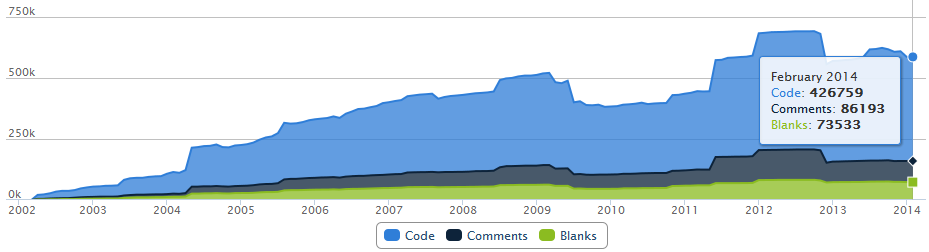
\includegraphics[width=\textwidth]{104_2014_w_Swierczewski_ohloh1.png}
  Figure 1. BOINC project – lines of code (data from 5 February 2014). Source: www.ohloh.net.
\end{figure}

\begin{figure}[b!]
  \centering
  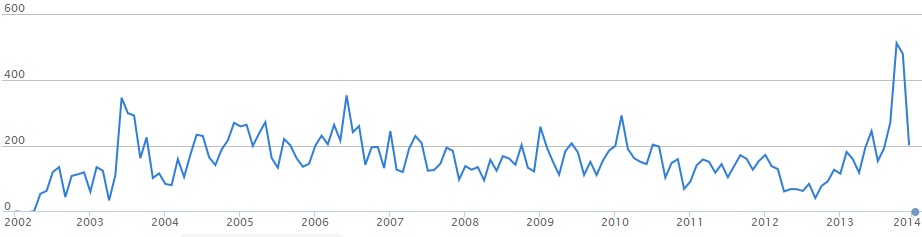
\includegraphics[width=\textwidth]{104_2014_w_Swierczewski_ohloh2.png}
  Figure 2. BOINC project – commits per month (data from 5 February 2014). Source: www.ohloh.net.
\end{figure}

Many projects using BOINC also provides their source code of applications or modules. Many users often try to optimize the application code so that it becomes more afficient . Sometimes such an improved software goes to the administrators of the project, and will be officially added and used as standard on all computers in the system. Also an interesting idea is to announca a competition for the best algorithm and its implementation in a particular programming language. This type of far more `social' solution was used recently in the project OPro\-ject@\-Ho\-me (www.oproject.info) in the subproject Weird Engine, which aims to find the so-called `weird numbers". After two months and receiving several interesting proposals, it turned out that the best solution has been sent by the Frenchman "--- Cedric Den Drijver. Basing on the new concept, a new version of the application has been created, which was several hundred times faster than the previous one. This change significantly contributed to the development of the project OPro\-ject@\-Ho\-me. With it you can now get far more results.

The only conclusion is that sometimes it is worth to describe a problem and ask for international help in finding a solution. If the issue is interesting, then, despite the fact, that the level of knowledge required to solve it, is very large and beyond knowledge of a statistical student, one can expect a response from some part of the world. For the creators of the BOINC projects, development can move in two directions. The first is calculations performed on thousands of computers and other, working on more and more perfect algorithms, which often are written not only by the official developers. Contribution to the project can be achieved by whole society, which forms around the project.

\end{document}

\documentclass[10pt, a5paper]{article}
\usepackage{pdfpages}
\usepackage{parallel}
\usepackage[T2A]{fontenc}
\usepackage{ucs}
\usepackage[utf8x]{inputenc}
\usepackage[polish,english,russian]{babel}
\usepackage{hyperref}
\usepackage{rotating}
\usepackage[inner=2cm,top=1.8cm,outer=2cm,bottom=2.3cm,nohead]{geometry}
\usepackage{listings}
\usepackage{graphicx}
\usepackage{wrapfig}
\usepackage{longtable}
\usepackage{indentfirst}
\usepackage{array}
\newcolumntype{P}[1]{>{\raggedright\arraybackslash}p{#1}}
\frenchspacing
\usepackage{fixltx2e} %text sub- and superscripts
\usepackage{icomma} % коскі ў матэматычным рэжыме
\PreloadUnicodePage{4}

\newcommand{\longpage}{\enlargethispage{\baselineskip}}
\newcommand{\shortpage}{\enlargethispage{-\baselineskip}}

\def\switchlang#1{\expandafter\csname switchlang#1\endcsname}
\def\switchlangbe{
\let\saverefname=\refname%
\def\refname{Літаратура}%
\def\figurename{Іл.}%
}
\def\switchlangen{
\let\saverefname=\refname%
\def\refname{References}%
\def\figurename{Fig.}%
}
\def\switchlangru{
\let\saverefname=\refname%
\let\savefigurename=\figurename%
\def\refname{Литература}%
\def\figurename{Рис.}%
}

\hyphenation{admi-ni-stra-tive}
\hyphenation{ex-pe-ri-ence}
\hyphenation{fle-xi-bi-li-ty}
\hyphenation{Py-thon}
\hyphenation{ma-the-ma-ti-cal}
\hyphenation{re-ported}
\hyphenation{imp-le-menta-tions}
\hyphenation{pro-vides}
\hyphenation{en-gi-neering}
\hyphenation{com-pa-ti-bi-li-ty}
\hyphenation{im-pos-sible}
\hyphenation{desk-top}
\hyphenation{elec-tro-nic}
\hyphenation{com-pa-ny}
\hyphenation{de-ve-lop-ment}
\hyphenation{de-ve-loping}
\hyphenation{de-ve-lop}
\hyphenation{da-ta-ba-se}
\hyphenation{plat-forms}
\hyphenation{or-ga-ni-za-tion}
\hyphenation{pro-gramming}
\hyphenation{in-stru-ments}
\hyphenation{Li-nux}
\hyphenation{sour-ce}
\hyphenation{en-vi-ron-ment}
\hyphenation{Te-le-pathy}
\hyphenation{Li-nux-ov-ka}
\hyphenation{Open-BSD}
\hyphenation{Free-BSD}
\hyphenation{men-ti-on-ed}
\hyphenation{app-li-ca-tion}

\def\progref!#1!{\texttt{#1}}
\renewcommand{\arraystretch}{2} %Іначай формулы ў матрыцы зліпаюцца з лініямі
\usepackage{array}

\def\interview #1 (#2), #3, #4, #5\par{

\section[#1, #3, #4]{#1 -- #3, #4}
\def\qname{LVEE}
\def\aname{#1}
\def\q ##1\par{{\noindent \bf \qname: ##1 }\par}
\def\a{{\noindent \bf \aname: } \def\qname{L}\def\aname{#2}}
}

\def\interview* #1 (#2), #3, #4, #5\par{

\section*{#1\\{\small\rm #3, #4. #5}}

\def\qname{LVEE}
\def\aname{#1}
\def\q ##1\par{{\noindent \bf \qname: ##1 }\par}
\def\a{{\noindent \bf \aname: } \def\qname{L}\def\aname{#2}}
}

\begin{document}
\title{Краткий обзор базовых лицензий СПО}
\author{Ирина Шубина, Минск, Беларусь\footnote{\url{klasy@tut.by}, \url{http://lvee.org/en/abstracts/104}}}}
\maketitle
\begin{abstract}
With this report we are going to make a quick and brief overview of the open-source licenses. Starting with the base ideas of the licensing we'll come to the most wirespread and most popular licenses used in the open-source software. Also one of the most important points of the report I would consider the differentiation of the permissive and copyleft licenses.
\end{abstract}
\section*{Введение}

\subsection*{Понятие лицензирования}

Лицензирование "--- соглашение сторон, по которому одна сторона предоставляет какие-либо права другой стороне. Лицензирование используется для защиты авторских прав.

Именно правила лицензирования диктуют различные права доступа и использования исходного кода в приложении к программному обеспечению.

\subsection*{Типы лицензирования}

Различают пермиссивные и копилефт лицензии.

\textbf{Пермиссивные лицензии} "--- это лицензии на программное обеспечение, которые практически не ограничивают свободу действий пользователей ПО и разработчиков, работающих с исходным кодом. По своему духу, распространение работы под пермиссивной лицензией схоже с помещением работы в общественное достояние, не требующее отказа от авторского права.

Идея \textbf{копилефт} состоит в том, что каждый, кто распространяет программу как с изменениями, так и без них, не вправе ограничивать свободу её дальнейшего распространения либо модификации.

\begin{itemize}
  \item \textbf{«Сильная»} copyleft лицензия  разрешает использовать код только программам, созданным под такой же лицензией.
  \item \textbf{«Слабая»} copyleft лицензия разрешает вносить любые изменения в код данной программы. Но она ставит условие, что другая программа, использующая данный код, будет строиться с указанием изначальной в качестве библиотеки. Тогда новая программа может выходить под любой другой лицензией.
\end{itemize}

В рамках данного типа лицензирования выделяют также полный и частичный копилефт.

\textbf{Полный копилефт} "--- все части программы (за исключением самой лицензии) могут модифицироваться и распространяться только под лицензией копилефта.

\textbf{Частичный копилефт} "--- программа может исключать несколько условий копилефт лицензии и при этом включать модификации в рамках какой-то не-копилефт лицензии. Или в некоторых случаях программа, распространяемая под такой лицензией, может следовать не всем принципам копилефта. Например, исключение, сделанное для некоторых программ для GPL связывания.

\section*{Краткий обзор лицензий}

\subsection*{GPL (General Public License)}

Стандартная Общественная Лицензия GNU (GNU General Public License, GNU GPL) "--- это свободная copyleft лицензия для программного обеспечения (ПО) и других видов произведений\footnotemark[1].

GNU GPL требует распространения с двоичными файлами (в том числе неизменными) исходного кода или письменного обязательства его предоставить (своего или чужого; способы зависят от версии лицензии).

Лицензии, созданные на базе GPL:
\begin{itemize}
  \item AGPL (Affero General Public License)
  \item LGPL (Lesser General Public License)
\end{itemize}

\subsection*{BSD (Berkley Software Distribution)}

Существуют две основные версии лицензии BSD, которые необходимо различать: «оригинальная» и так называемая «модифицированная» (вторую в англоязычной литературе часто называют New BSD License). Данная лицензия является пермиссивной.

Лицензия BSD допускает проприетарное коммерческое использование ПО. Для ПО, выпущенного под этой лицензией, допускается встраивание в проприетарные коммерческие продукты. Работы, основанные на таком ПО, даже могут распространяться под проприетарными лицензиями (но всё же обязаны соответствовать требованиям лицензии). Наиболее заметные примеры таких программ "--- использование сетевого кода BSD в продуктах корпорации Microsoft, а также использование многих компонентов FreeBSD в операционной системе Mac OS X.

\subsection*{Apache Software License}

Лицензия Apache даёт пользователю право использовать программное обеспечение для любых целей, свободно распространять, изменять, и распространять изменённые копии, за исключением названия.

Данная лицензия не ставит условием неизменность лицензии распространения программного обеспечения, и не настаивает даже на сохранении его открытого статуса. Единственным условием, накладываемым лицензией Apache, является информирование получателя о факте использования исходного кода. В противоположность copyleft-лицензиям, получатель модифицированной версии не обязательно получает все права, изначально предоставляемые лицензией Apache.

В каждом лицензируемом файле должна быть сохранена вся исходная информация о копирайтах или патентах, в каждый изменённый файл должна добавляться информация о проведённых изменениях.

\section*{Совместимость лицензий}

\textbf{Совместимость} "--- понятие, возникающее при попытке комбинирования двух и более лицензий. Совместимость определяет непосредственно возможность комбинации одной лицензии с другими. Совместимость может варьироваться в зависимости от типа лицензии, а версии самой лицензии. Различают GPL-совсемстимые и GPL-несовместимые лицензии. Также нужно отметить возможность сочетать закрытые (или проприетарные) лицензии с открытыми.

Ссылка на ресурс, где можно посмотреть совместимость лицензий: http://www.tldrlegal.com/compare

\footnotetext[1]{Взято из Неофициального Перевода GNU GPLv3 (http://code.google.com/p/gpl3rus/wiki/LatestRelease)}\footnotetext[2]{Большая часть мариала основана на статьях Википедии (wikipedia.org).}
\end{document}

\documentclass [10pt, a5paper]{article}
\usepackage{pdfpages}
\usepackage{parallel}
\usepackage[T2A]{fontenc}
\usepackage{ucs}
\usepackage[utf8x]{inputenc}
\usepackage[polish,english,russian]{babel}
\usepackage{hyperref}
\usepackage{rotating}
\usepackage[inner=2cm,top=1.8cm,outer=2cm,bottom=2.3cm,nohead]{geometry}
\usepackage{listings}
\usepackage{graphicx}
\usepackage{wrapfig}
\usepackage{longtable}
\usepackage{indentfirst}
\usepackage{array}
\newcolumntype{P}[1]{>{\raggedright\arraybackslash}p{#1}}
\frenchspacing
\usepackage{fixltx2e} %text sub- and superscripts
\usepackage{icomma} % коскі ў матэматычным рэжыме
\PreloadUnicodePage{4}

\newcommand{\longpage}{\enlargethispage{\baselineskip}}
\newcommand{\shortpage}{\enlargethispage{-\baselineskip}}

\def\switchlang#1{\expandafter\csname switchlang#1\endcsname}
\def\switchlangbe{
\let\saverefname=\refname%
\def\refname{Літаратура}%
\def\figurename{Іл.}%
}
\def\switchlangen{
\let\saverefname=\refname%
\def\refname{References}%
\def\figurename{Fig.}%
}
\def\switchlangru{
\let\saverefname=\refname%
\let\savefigurename=\figurename%
\def\refname{Литература}%
\def\figurename{Рис.}%
}

\hyphenation{admi-ni-stra-tive}
\hyphenation{ex-pe-ri-ence}
\hyphenation{fle-xi-bi-li-ty}
\hyphenation{Py-thon}
\hyphenation{ma-the-ma-ti-cal}
\hyphenation{re-ported}
\hyphenation{imp-le-menta-tions}
\hyphenation{pro-vides}
\hyphenation{en-gi-neering}
\hyphenation{com-pa-ti-bi-li-ty}
\hyphenation{im-pos-sible}
\hyphenation{desk-top}
\hyphenation{elec-tro-nic}
\hyphenation{com-pa-ny}
\hyphenation{de-ve-lop-ment}
\hyphenation{de-ve-loping}
\hyphenation{de-ve-lop}
\hyphenation{da-ta-ba-se}
\hyphenation{plat-forms}
\hyphenation{or-ga-ni-za-tion}
\hyphenation{pro-gramming}
\hyphenation{in-stru-ments}
\hyphenation{Li-nux}
\hyphenation{sour-ce}
\hyphenation{en-vi-ron-ment}
\hyphenation{Te-le-pathy}
\hyphenation{Li-nux-ov-ka}
\hyphenation{Open-BSD}
\hyphenation{Free-BSD}
\hyphenation{men-ti-on-ed}
\hyphenation{app-li-ca-tion}

\def\progref!#1!{\texttt{#1}}
\renewcommand{\arraystretch}{2} %Іначай формулы ў матрыцы зліпаюцца з лініямі
\usepackage{array}

\def\interview #1 (#2), #3, #4, #5\par{

\section[#1, #3, #4]{#1 -- #3, #4}
\def\qname{LVEE}
\def\aname{#1}
\def\q ##1\par{{\noindent \bf \qname: ##1 }\par}
\def\a{{\noindent \bf \aname: } \def\qname{L}\def\aname{#2}}
}

\def\interview* #1 (#2), #3, #4, #5\par{

\section*{#1\\{\small\rm #3, #4. #5}}

\def\qname{LVEE}
\def\aname{#1}
\def\q ##1\par{{\noindent \bf \qname: ##1 }\par}
\def\a{{\noindent \bf \aname: } \def\qname{L}\def\aname{#2}}
}

\begin{document}
\title{Кандалы прогресса: авторское право и научные публикации}
\author{Антон Литвиненко, Киев, Украина\footnote{\url{tenebrosus.scriptor@gmail.com}, \url{http://lvee.org/en/abstracts/109}}}
\maketitle
\begin{abstract}
Copyright treats scientific publication equal to regular work of art, ignoring its specific nature, that gives some signs of natural monopolies to scientific publishing houses. This severely compli\-cates exchange of scientific information and, so, slows down the worldwide research. Present issues of access to publications to\-gether with some present and theoretical methods of their solu\-tion are discussed.
\end{abstract}
\subsection*{Открытость как основа мировой исследовательской деятельности}

Во времена Средневековья и более ранних цивилизаций, когда наука в современном виде еще не сформировалась, а объем знаний о мире был невелик, исследователи тщательно скрывали свои результаты, распространяя их максимум в узком круге учеников, зачастую придумывая специальные обозначения и шифры. При экспоненциальном нарастании количества информации в мире вообще и научного знания в частности наука перестала быть делом одиночек-энциклопедистов и вынуждена основываться на тесном сотрудничестве и интенсивном обмене информацией между исследователями и их группами. Каждая научная работа добавляет незначительный фрагмент информации в общую структуру научного знания, общий объем которого давно невозможно изучить, а тем более исследовать одному человеку. При этом, фактически, работа, не обнародованная в общедоступных источниках, не существует для научной общественности.

Доступность для исследователя научных работ его коллег исторически составляла некоторую проблему по ряду технических причин: необходимость физической доставки экземпляров журналов и книг, языковой барьер, сложность поиска, политические аспекты (например, «железный занавес»). Для решения этих проблем с переменным успехом применялся ряд технических подходов (например, реферативные журналы для облегчения поиска), пока они не были фактически решены за счет компьютеризации, четкого доминирования английского языка и краха биполярной политической системы.

Однако, на пути прогресса встали вопросы авторского права.

\subsection*{Особенности авторского права на научные публикации}

Фундаментальная информация о природе, получаемая в процессе научного познания, является общественным достоянием. Тем не менее, при работе исследования создается и продукт, который может становиться объектом интеллектуальной собственности. Это касается:
\begin{itemize}
  \item Разработки новых изобретений; устройств, методов, материалов и прочих результатов, которые могут быть запатентованы;
  \item Баз данных научной информации, которые, не обладая правами на содержащуюся информацию, обладают правами на ее компиляции и результаты поиска;
  \item Авторское право на научные публикации.
\end{itemize}

С точки зрения авторского права, научные публикации являются обычными литературными произведениями.

\subsection*{Принципиальные отличия между научной публикацией и литературным произведением в контексте авторского права}
\begin{enumerate}
  \item Литературное произведение можно опубликовать с помощью любой организации, способной подготовить его к печати (при необходимости) и физически создать нужное количество экземпляров. Именитость издания может иметь некоторое значение для дальнейшей судьбы произведения, но основным является физическое наличие тиража. В то же время, для научного произведения место опубликования имеет критическое значение:\begin{itemize}
  \item Научное произведение должно пройти рецензирование в той или оной форме. Именитость места публикации (издательства, периодического издания, представительства конференции и т.\,д.) играет значительную роль и выступает показателем качества произведения (в том числе через систему наукометрических параметров, характеризующих место публикации "--- например, импакт"=фактор журнала).
  \item Авторитет места публикации влияет на принятие работы как научной, а также ее добавление в общую структуру научного знания "--- будут ли другие исследователи читать работу, воспримут ли ее всерьез, будет ли она доступна в научных поисковых системах.
  \item В некоторых случаях в качестве приемлемых научных работ воспринимаются только опубликованные в местах из определенного авторизованного списка (например, \linebreak списки ВАКов).
  \item Выход на рынок научных публикаций достаточно затруднен, так как малоизвестному издателю сложно претендовать на поступление для публикации интересных высококачественных работ.
\end{itemize}


  \item Первичные научные работы (по материалам оригинальных исследований), как правило, содержат достаточно уникальную информацию, которая редко где-либо дублируется полностью. Таким образом, необходимость доступа к конкретной публикации (а в процессе текущих работ теоретически может понадобиться доступ к любой ранее опубликованной работе) может быть критической без возможности замены какой-либо другой публикацией.
  \item Как правило, исследователь не получает значительного дохода от продажи своих научных публикаций (часто не получает его вообще), мотивы публикации и распространения своих трудов более нематериальны.
\end{enumerate}

Таким образом, рынок научного издательства имеет черты природной монополии (олигополии), в котором интерес издателя и автора существенно различен. Однако, это совершенно игнорируется при юридическом регулировании.

\subsection*{Типичная политика научных издательств}

\begin{enumerate}
  \item Продается подписка на печатный журнал и/или на онлайн-доступ к электронным версиям статей за все время или определенный период; а также продается онлайн-доступ к отдельным публикациям при отсутствии общей подписки;
  \item Подписка стоит дорого. Например, годовая подписка на журнал Angewandte Chemie стоит \$11529 (печатный + онлайн) [1]. А таких журналов только по химии десятки самых важных, а по широкому набору дисциплин (например, для научной библиотеки) сотни и тысячи. Доступ же к единичной статье стоит десятки долларов. Так, библиотека Гарварда в 2013 году сделала заявление о непомерных расходах на журнальные подписки, призвав ученых публиковаться в бесплатно распространяемых журналах [2].
  \item Подписки могут продаваться сразу на группу журналов. Фактически, часть журналов может продаваться в довесок.
  \item Гонорары авторам невелики или вовсе отсутствуют.
  \item Рецензенты не получают денег за работу.
  \item Условия лицензионных соглашений предусматривают передачу практически всех прав издательству.
  \item Высокая стоимость не гарантирует однозначно высокого качества научных публикаций.
  \item В последнее время большинство научных журналов было скуплено тремя большими издательскими домами: Wiley, Elsevier, Springer.
\end{enumerate}

Издатель научных публикаций торгует воздухом, пользуясь монопольным положением. Такая ситуация ведет к затруднению научных исследований, повышению порога вхождения в научную деятельность, недоступности результатов оригинальных исследований для широких масс интересующихся людей.

В последние годы это (а также ряд других причин вроде поддержки SOPA и PIPA) вызвало даже попытки «бунта» среди ученых, в том числе и весьма известных, "--- в частности, бойкот издательства Elsevier [3,4].

\subsection*{Методы борьбы}

\begin{enumerate}
  \item Заграница нам поможет. Ссылки, которые нужно скачать, направляются знакомым «утекшим мозгам» или временно стажирующимся/работающим за бугром коллегам или друзьям. Они скачивают статью, пользуясь местной подпиской.
  \item Расширенные версии предыдущих. Сообщества для реквестов вроде жжшного pdf.livejournal.com, межбиблиотечные подписки и т.д.
  \item Связка проектов sci-hub.org и libgen.org. Первый представляет собой систему прокси с парсерами и прочими техническими дополнениями для автоматического доступа к журналам через компьютеры в западных университетах. Второй "--- огромный фонд научных публикаций, ставящий цель собрать большинство научных публикаций в истории мировой науки вообще. Скачанные через sci-hub статьи автоматически попадают в libgen, при повторной скачке предлагается уже готовая копия. При неудачной попытке поиска через libgen предлагается открыть статью через sci-hub.
  \item Опция издательства "--- авторы платят за публикацию, после чего она становится открытой всем.
  \item Open-access журналы "--- аналог предыдущего, но применяется для всего журнала. Как правило, не имеет печатной версии. В то же время, могут финансироваться как авторами, так и из других источников. Некоторые исследователи критикуют низкое качество рецензирования, но проводимые ими исследования не вполне строгие (традиционные журналы страдают теми же проблемами) [3,5], и эти проблемы могут быть объяснены новизной явления. В качестве примера open-access журнала можно привести PLOS Biology, который взнимает с авторов зависящую от страны плату и публикует работу под лицензией Creative Commons CC-BY [6].
  \item Тома журналов выкачиваются постатейно ботами и выкладываются на торрентах.
  \item Максимально используются оставшиеся у автора права "--- рассылка небольшого числа авторских копий, публикация препринтов (не все журналы). Публикация препринтов эффективна в интеграции с Google Scholar (рядом со ссылкой на статью позволяет скачать найденный препринт с другого адреса).
  \item Использование временного открытия некоторых статей во время рекламных кампаний, доступа по паролям для рецензентов через проприетарные поисковики и прочих лазеек.
\end{enumerate}

Таким образом, большинство имеющихся методов борьбы являются откровенно пиратскими, а существующие легально не решают целостной проблемы (open access распространяется только на работы, явно опубликованные по этой модели).

Для существенного прогресса в вопросе авторских прав на научные работы следует разрабатывать и вносить изменения в законодательство об авторском праве, выделяя научные публикации в особый вид произведений со специальным регулированием. Например, существенное уменьшение (до нескольких лет) времени перехода в общественное достояние.

Таким образом, несмотря на принципиальную приверженность открытости информации, научному сообществу еще только предстоит пройти путь по либерализации недопустимой ситуации с авторскими правами, который уже успешно проходит общество программистское.

P.\,S. Во время обсуждения доклада слушателями были названы еще некоторые цифровые хранилища и библиотеки, из которых можно бесплатно или за разумную цену поличить желаемую литературу по определенным областям знаний. В частности, сайт CiteSeerX [7] (спасибо Алексею Чеусову).

\begin{thebibliography}{9}
 \bibitem{L1} \url{http://ordering.onlinelibrary.wiley.com/subs.asp?ref=1521-3757&doi=10.1002/(ISSN)1521-3757}
 \bibitem{L2} \url{http://www.vestifinance.ru/articles/22492/print}
 \bibitem{L3} \url{http://theoryandpractice.ru/posts/8440-znaniya-dlya-vsekh}
 \bibitem{L4} \url{http://www.svoboda.org/content/article/24892099.html}
 \bibitem{L5} \url{http://habrahabr.ru/company/cyberleninka/blog/197946/}
 \bibitem{L6} \url{http://www.plosbiology.org/static/information}
 \bibitem{L7} \url{http://citeseerx.ist.psu.edu}
\end{thebibliography}
\end{document}

\documentclass[10pt, a5paper]{article}
\usepackage{pdfpages}
\usepackage{parallel}
\usepackage[T2A]{fontenc}
\usepackage{ucs}
\usepackage[utf8x]{inputenc}
\usepackage[polish,english,russian]{babel}
\usepackage{hyperref}
\usepackage{rotating}
\usepackage[inner=2cm,top=1.8cm,outer=2cm,bottom=2.3cm,nohead]{geometry}
\usepackage{listings}
\usepackage{graphicx}
\usepackage{wrapfig}
\usepackage{longtable}
\usepackage{indentfirst}
\usepackage{array}
\newcolumntype{P}[1]{>{\raggedright\arraybackslash}p{#1}}
\frenchspacing
\usepackage{fixltx2e} %text sub- and superscripts
\usepackage{icomma} % коскі ў матэматычным рэжыме
\PreloadUnicodePage{4}

\newcommand{\longpage}{\enlargethispage{\baselineskip}}
\newcommand{\shortpage}{\enlargethispage{-\baselineskip}}

\def\switchlang#1{\expandafter\csname switchlang#1\endcsname}
\def\switchlangbe{
\let\saverefname=\refname%
\def\refname{Літаратура}%
\def\figurename{Іл.}%
}
\def\switchlangen{
\let\saverefname=\refname%
\def\refname{References}%
\def\figurename{Fig.}%
}
\def\switchlangru{
\let\saverefname=\refname%
\let\savefigurename=\figurename%
\def\refname{Литература}%
\def\figurename{Рис.}%
}

\hyphenation{admi-ni-stra-tive}
\hyphenation{ex-pe-ri-ence}
\hyphenation{fle-xi-bi-li-ty}
\hyphenation{Py-thon}
\hyphenation{ma-the-ma-ti-cal}
\hyphenation{re-ported}
\hyphenation{imp-le-menta-tions}
\hyphenation{pro-vides}
\hyphenation{en-gi-neering}
\hyphenation{com-pa-ti-bi-li-ty}
\hyphenation{im-pos-sible}
\hyphenation{desk-top}
\hyphenation{elec-tro-nic}
\hyphenation{com-pa-ny}
\hyphenation{de-ve-lop-ment}
\hyphenation{de-ve-loping}
\hyphenation{de-ve-lop}
\hyphenation{da-ta-ba-se}
\hyphenation{plat-forms}
\hyphenation{or-ga-ni-za-tion}
\hyphenation{pro-gramming}
\hyphenation{in-stru-ments}
\hyphenation{Li-nux}
\hyphenation{sour-ce}
\hyphenation{en-vi-ron-ment}
\hyphenation{Te-le-pathy}
\hyphenation{Li-nux-ov-ka}
\hyphenation{Open-BSD}
\hyphenation{Free-BSD}
\hyphenation{men-ti-on-ed}
\hyphenation{app-li-ca-tion}

\def\progref!#1!{\texttt{#1}}
\renewcommand{\arraystretch}{2} %Іначай формулы ў матрыцы зліпаюцца з лініямі
\usepackage{array}

\def\interview #1 (#2), #3, #4, #5\par{

\section[#1, #3, #4]{#1 -- #3, #4}
\def\qname{LVEE}
\def\aname{#1}
\def\q ##1\par{{\noindent \bf \qname: ##1 }\par}
\def\a{{\noindent \bf \aname: } \def\qname{L}\def\aname{#2}}
}

\def\interview* #1 (#2), #3, #4, #5\par{

\section*{#1\\{\small\rm #3, #4. #5}}

\def\qname{LVEE}
\def\aname{#1}
\def\q ##1\par{{\noindent \bf \qname: ##1 }\par}
\def\a{{\noindent \bf \aname: } \def\qname{L}\def\aname{#2}}
}

\begin{document}
\title{Опыты над людьми и Octave: FOSS-based GSR measurements}
\author{Ольга Карабутова, Minsk, Belarus}
\maketitle
\begin{abstract}
The paper describes practical experience of creating a biometrical device to evaluate user’s stress level. Signs specific to stress are considered as well as the device prototype and intermediate research results. Free/libre open-source software used to evaluate and analyse raw biometric data is covered.
\end{abstract}
\subsection*{Вступление}

С каждым днем различные устройства, использующие биометрические данные (фитнес-гаджеты, сканеры отпечатков пальцев, умные часы, умные очки, одежда, протезы, управляемые силой мысли, нейрокомпьютерные интерфейсы) находят все более широкое применение, а сами устройства становятся меньше и удобнее для повседневного использования.

Перед нами стояла задача  создания биометрического устройства, которое могло бы отслеживать уровень стресса  человека в течение дня, недели.  Хотя обычно человек сам в состоянии определить, находится сейчас он в стрессовом состоянии или нет, но он далеко не всегда способен объективно оценить стрессовую  нагрузку на свой организм, тем более, не всегда очевидны причины стресса.

\subsection*{Стресс}

Под стрессом (от англ. stress "--- нажим, напряжение) понимают общую реакцию организма на физическое или психологическое воздействие, выводящее его из состояния равновесия (нарушающее гомеостаз), а также соответствующее состояние нервной системы и организма в целом.
«Изобретатель» стресса канадский эндокринолог Ганс Салье доказал, что стресс ведет к истощению организма и к очень многим нарушениям здоровья.

Реакцию организма на стресс можно выразить фразой «дерись или беги». За большинство физиологических изменений, отвечают две нейроэндокринные системы, управляемых гипоталамусом: симпатической и парасимпатической. Симпатическая нервная система подготавливает организм к атаке, обеспечивая выброс в кровь глюкозы, увеличение кислорода в крови и артериального давления, сердцебиения, расширяет зрачок, активирует железы и мускулатуру, сокращает ток периферических сосудов, а также подавляет деятельность большинства внутренних органов, такие как пищеварение. Действие парасимпатической системы во многом противоположно. Поэтому можно выделить стандартные признаки, сопутствующие стрессовой ситуации:

\begin{itemize}
  \item артериальное давление
  \item содержание сахара и кислорода в крови
  \item повышение частоты сердцебиения, учащение дыхания
  \item расширение зрачков
  \item специфическое сокращение лицевых нервов (мимика)
  \item уменьшение слюноотделения
\end{itemize}

С точки зрения использования в конечном устройстве для выявления стресса нас интересуют в первую очередь метрики, пригодные для неинвазивного измерения и обладающие при этом достаточной достоверностью.

Ряд исследований показывает, что для детектирования стресса достаточно одного датчика кожно-гальванической реакции (Galvanic Skin Response или GSR).

\begin{figure}[h!]
  \centering
  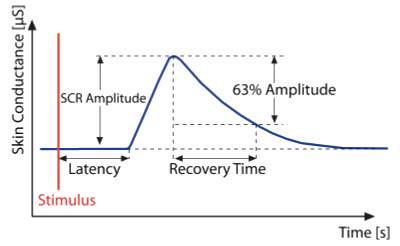
\includegraphics{107_2014_w_Karabutova_plot.png}
\end{figure}

GSR "--- биоэлектрическая реакция, обусловленная деятельностью потовых желез. Если приложить к коже электрическое напряжение, то между двумя участками кожи можно замерить электрическое сопротивление или проводимость. Во время стрессового воздействия потовые железы кожи выделяют микрочастицы пота, в результате чего сопротивление кожи меняется.

На рисунке показана идеальная реакция на стрессовый стимул, обозначенный красной линией с подписью «Stimulus». Можно заметить временную задержку отклика (Latency) и последующее время восстановления (Recovery), т.е. адаптации к новому гомеостазу или релаксации после точечного стресса.

\subsection*{Устройство}

Разработка включает две части: носимое устройство в виде браслета и программное обеспечение, устанавливаемое на персональный компьютер или мобильное устройство.

Носимое устройство включает следующие части:

\begin{itemize}
  \item датчик GSR
  \item акселерометр
  \item микропроцессор
  \item память
  \item RF-модуль (Bluetooth Low Energy)
  \item устройство питания (батарея CR2032 или литий-полимерный аккумулятор)
\end{itemize}

\begin{figure}[b!]
  \centering
  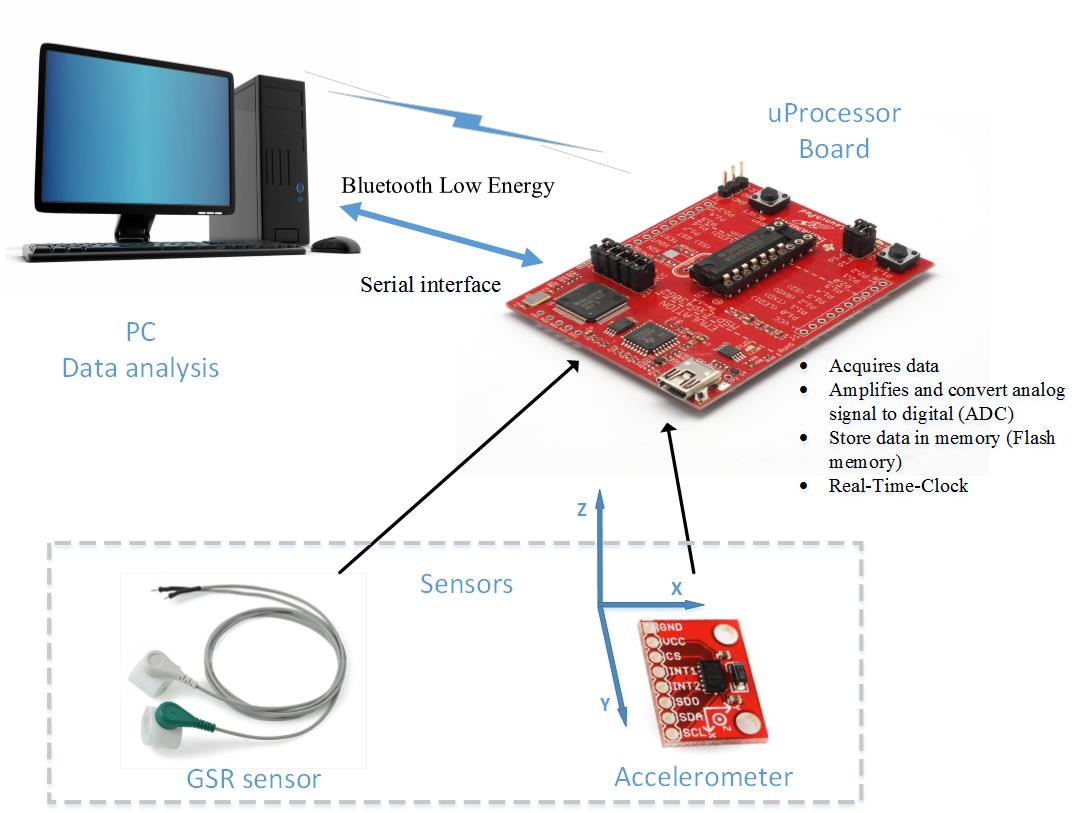
\includegraphics[width=0.8\textwidth]{107_2014_w_Karabutova_struct.png}
\end{figure}

Биометрия считывается с аналоговых датчиков, усиливается, конвертируется в цифровой сигнал. Далее показания агрегируются в памяти, находящейся на устройстве. При портативном ношении данные собираются на устройстве за продолжительный период времени. Также они могут передаваться в режиме реального времени на персональный компьютер или мобильное устройство для обработки "--- как по интерфейсу USB, так и через беспроводной интерфейс Bluetooth Low Energy, который широко используется в медицинских устройствах.

Для обработки данных на PC использован GNU Octave.

\subsection*{Методика тестирования}

Для проверки работоспособности прибора использовалась серия тестов следующего вида. После закрепления датчиков подопытному давался адаптационный период не менее 15 минут. Далее испытуемый подвергается стрессовым воздействиям, которые следовали одно за другим в случайном порядке. Воздействия проводились с перерывом в 20—30 минут. Между последним стрессовым воздействием и завершением предусматривалась пауза не менее 10—15 минут. Общая продолжительность одной сессии составляет 1—3 часа.

Датчики GSR крепятся на двух пальцах одной руки или на запястье подопытного, но должны быть разнесены минимум на 1 сантиметр расстояния между ними, с обеспечением плотного контакта. Плотность контакта на пальцах обеспечивается заводским креплением на «липучке», а на запястье "--- креплением на резинке с регулируемой длиной браслета. Дополнительно на теле человека закрепляется акселерометр.

В качестве типов стрессовой нагрузки применялись следующие:
\begin{center}
  %\centering
  \begin{longtable}{P{10em}|P{20em}}
    \hline
    Физическое воздействие & Физические упражнения \\
     & Изменение температуры в помещении \\
    \hline
    Когнитивная нагрузка & Решение интересных, но не тривиальных задач \\[-2ex]
     & Прохождение/выполнение задач вне компетенции на время \\[-2ex]
     & Соревновательные игры \\
    \hline
    Эмоциональная нагрузка & Видеоролики или материалы, вызывающие эмоциональный отклик \\
     & Обсуждение событий, вызывающих радость, положительные эмоции \\
     & Требование отчета вышестоящим начальником (этот тест показал слабую эффективность) \\
     & Ситуация экзамена \\
    \hline
  \end{longtable}
\end{center}
Данные с датчиков сохранялись в cvs-файл и затем обрабатывались в Octave. Там же обработанные данные пропускались через алгоритм, выдающий на выходе, когда у человека был стресс (по показаниям GSR), и был ли он вызван физической активностью или нет (по показаниям акселерометра).

\begin{figure}[h!]
  \centering
  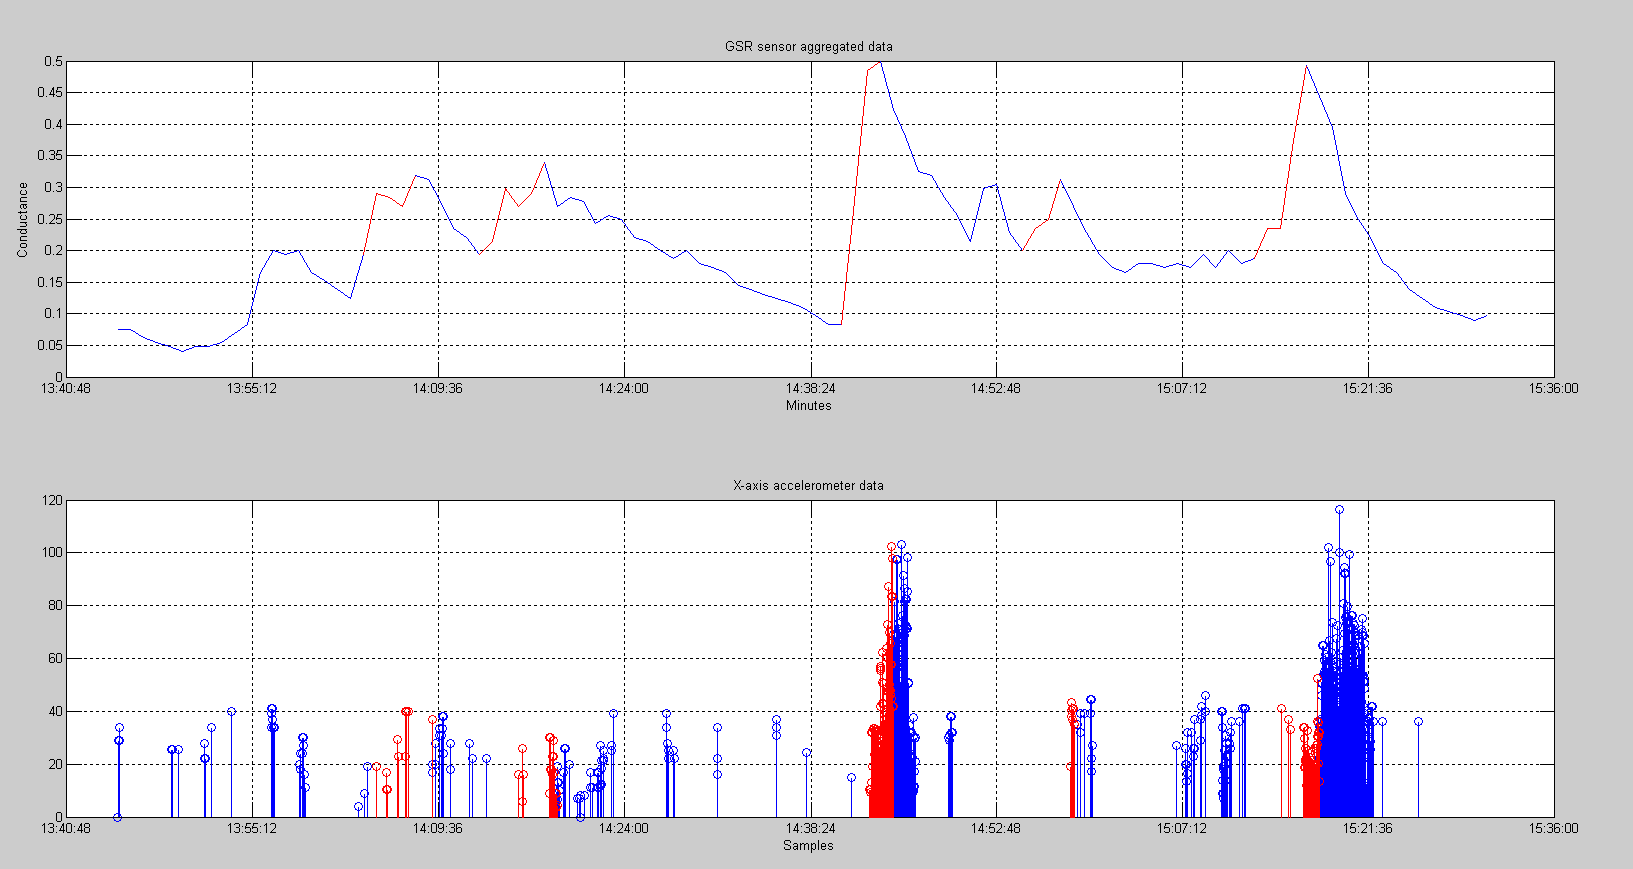
\includegraphics[width=\textwidth]{107_2014_w_Karabutova_data.png}
\end{figure}

\newpage
Параллельно все происходящее во время опытов тщательно документировалось наблюдателем. Пример журнала:
\begin{longtable}{P{5em}|P{25em}}
\hline
13.57  &  Испытуемый разговаривает по телефону \linebreak
Виден пик повышения GSR, но как стресс программа это не выделила (не достаточно существенное отклонение от общего уровня GSR) \\
14.05  &  Игра «Морской бой» с ограничением по времени \\
14.09   &  Окончание игры \\
14.10   &  Обсуждение игры и тактик. (Испытуемый выиграл) \\
14.44  &  Физическое упражнение  «бег на месте» \linebreak
Стресс, вызванный физической активностью испытуемого, легко отличить по показаниям акселерометра \\
14.45  &  Завершение физических упражнений \\
15.00  &  Включение обогревателя в комнате \\
15.16  &  Выполнение разнообразных физических упражнений \\
15.21  &  Завершение физических упражнений \\
\hline
\end{longtable}

\subsection*{Результаты испытаний}

Тестирование показало, что стресс, вызванный физической нагрузкой, детектируется 100\%. Что касается прочих причин, было сложно иногда создать однозначно стрессовую ситуацию для подопытного.
Например, ситуация отчета перед начальством не всегда вызывала у подопытного волнение (подопытному было известно, что он в ситуации «теста» и ситуация создана искусственно).
Тем не менее, у разработчика, который также иногда выступал в роли подопытного, сообщение о визите вышестоящего начальства, как и сам визит, однозначно повышало регистрируемый уровень стресса.

Игровые ситуации дают однозначный результат, как и во время игры, так и при последующих обсуждениях результатов и стратегий. Аналогично дело обстоит и с просмотром видеоматериалов, вызывающих с высокой долей вероятности эмоциональный отклик у реципиентов.

\subsection*{Octave}

GNU Octave "--- свободная система для математических вычислений, использующая совместимый с MATLAB язык высокого уровня.
По сути, Octave "--- это свободный клон MATLAB, благодаря чему и динамически подгружаемые модули (*.m-файлы), и пользовательские функции можно очень легко портировать из одной среды в другую.

В среде профессиональных исследователей MATLAB занимает лидирующие позиции (благодаря крайне обширному набору вычислительных функций практически для всех областей применения) а к его свободным клонам часто относятся с предубеждением. Однако по нашему опыту GNU Octave оказался чрезвычайно мощным математическим инструментом, с помощью которого можно экспериментировать, моделировать устройства и обрабатывать цифровые данные.

Не в последнюю очередь это достигается благодаря тому, что Octave позволяет подключать сторонние утилиты, а также общие или предметно-ориентированные библиотеки функций для вычислений. 
Например, для построения графиков по умолчанию Octave использует Gnuplot, хотя также есть на выбор не менее 5 альтернативных графических пакетов.

Сторонняя библиотека Octave-forge включает множество пакетов, среди которых для решения класса задач анализа биометрических данных нами были отобраны следующие:

\textbf{Для получения данных из подключаемых устройств:}

\begin{itemize}
  \item \textbf{instrument-control} позволяет взаимодействовать с внешними устройствами через последовательный и параллельный порты, I²C, TCP/IP, интерфейсы GPIB, VXI11 и USBTMC.
  \item \textbf{communications} "--- передача цифровых данных, кодов коррекции ошибок ECC, модуляции и поля Галуа.
\end{itemize}

\textbf{Для цифровой обработки сигнала:}

\begin{itemize}
  \item \textbf{signal} "--- наборы функций для обработки сигналов (а также обработки изображений, проектирования цифровых фильтров и систем связи -- БПФ, фильтры различных порядков).
  \item \textbf{ltfat} "--- библиотека частотно-временного анализа сигналов. Позволяет производить большое количество линейных преобразований, включая преобразование Габора и вейвлет-преобразование, а так же шаблоны для конструирования окон (моделирование фильтров) и утилиты для манипулирования коэффициентами.
\end{itemize}

\textbf{Для статистики, анализа данных и машиного обучения:}

\begin{itemize}
  \item \textbf{nan} "--- набор утилит для статистики и машинного обучения, работает как с Octave, так и с Matlab, умеет обрабатывать как непрерывные данные, так и данные с пропущенными значениями.
  \item \textbf{mvn} "--- кластеризация многомерного нормального распределения
  \item \textbf{fuzzy-logic-toolkit} позволят создавать экспертные системы на основе нечеткой логики, проводить кластеризацию нечеткими алгоритмами, а также проектировать нечеткие нейронные сети.
  \item \textbf{fl-core} содержит базовые функции для нечеткой логики.
  \item \textbf{queueing} содержит набор функций в том числе и для анализа цепей Маркова
\end{itemize}

В итоге для решения нашей задачи был задействован меньший набор пакетов Octave для построения эффективной обработки данных и ее статистического анализа (преимущественно использовались пакеты signal). Определенно мог быть задействован пакет instrument-control для приема данных на ПК.
Но Octave "--- поистине мощный математический инструмент, с помощью которого можно экспериментировать, моделировать устройства и обрабатывать цифровые данные.

\end{document}

\documentclass[10pt, a5paper]{article}
\usepackage{pdfpages}
\usepackage{parallel}
\usepackage[T2A]{fontenc}
\usepackage{ucs}
\usepackage[utf8x]{inputenc}
\usepackage[polish,english,russian]{babel}
\usepackage{hyperref}
\usepackage{rotating}
\usepackage[inner=2cm,top=1.8cm,outer=2cm,bottom=2.3cm,nohead]{geometry}
\usepackage{listings}
\usepackage{graphicx}
\usepackage{wrapfig}
\usepackage{longtable}
\usepackage{indentfirst}
\usepackage{array}
\newcolumntype{P}[1]{>{\raggedright\arraybackslash}p{#1}}
\frenchspacing
\usepackage{fixltx2e} %text sub- and superscripts
\usepackage{icomma} % коскі ў матэматычным рэжыме
\PreloadUnicodePage{4}

\newcommand{\longpage}{\enlargethispage{\baselineskip}}
\newcommand{\shortpage}{\enlargethispage{-\baselineskip}}

\def\switchlang#1{\expandafter\csname switchlang#1\endcsname}
\def\switchlangbe{
\let\saverefname=\refname%
\def\refname{Літаратура}%
\def\figurename{Іл.}%
}
\def\switchlangen{
\let\saverefname=\refname%
\def\refname{References}%
\def\figurename{Fig.}%
}
\def\switchlangru{
\let\saverefname=\refname%
\let\savefigurename=\figurename%
\def\refname{Литература}%
\def\figurename{Рис.}%
}

\hyphenation{admi-ni-stra-tive}
\hyphenation{ex-pe-ri-ence}
\hyphenation{fle-xi-bi-li-ty}
\hyphenation{Py-thon}
\hyphenation{ma-the-ma-ti-cal}
\hyphenation{re-ported}
\hyphenation{imp-le-menta-tions}
\hyphenation{pro-vides}
\hyphenation{en-gi-neering}
\hyphenation{com-pa-ti-bi-li-ty}
\hyphenation{im-pos-sible}
\hyphenation{desk-top}
\hyphenation{elec-tro-nic}
\hyphenation{com-pa-ny}
\hyphenation{de-ve-lop-ment}
\hyphenation{de-ve-loping}
\hyphenation{de-ve-lop}
\hyphenation{da-ta-ba-se}
\hyphenation{plat-forms}
\hyphenation{or-ga-ni-za-tion}
\hyphenation{pro-gramming}
\hyphenation{in-stru-ments}
\hyphenation{Li-nux}
\hyphenation{sour-ce}
\hyphenation{en-vi-ron-ment}
\hyphenation{Te-le-pathy}
\hyphenation{Li-nux-ov-ka}
\hyphenation{Open-BSD}
\hyphenation{Free-BSD}
\hyphenation{men-ti-on-ed}
\hyphenation{app-li-ca-tion}

\def\progref!#1!{\texttt{#1}}
\renewcommand{\arraystretch}{2} %Іначай формулы ў матрыцы зліпаюцца з лініямі
\usepackage{array}

\def\interview #1 (#2), #3, #4, #5\par{

\section[#1, #3, #4]{#1 -- #3, #4}
\def\qname{LVEE}
\def\aname{#1}
\def\q ##1\par{{\noindent \bf \qname: ##1 }\par}
\def\a{{\noindent \bf \aname: } \def\qname{L}\def\aname{#2}}
}

\def\interview* #1 (#2), #3, #4, #5\par{

\section*{#1\\{\small\rm #3, #4. #5}}

\def\qname{LVEE}
\def\aname{#1}
\def\q ##1\par{{\noindent \bf \qname: ##1 }\par}
\def\a{{\noindent \bf \aname: } \def\qname{L}\def\aname{#2}}
}

\begin{document}
\title{Реализация UEFI SecureBoot в ALT Linux}
\author{Михаил Шигорин, Киев, Украина\footnote{\url{mike@altlinux.org}, \url{http://lvee.org/en/abstracts/117}}}
\maketitle
\begin{abstract}
There are many misunderstandings and myths related to UEFI in general and SecureBoot extension in particular; I've implemented both within ALT Linux distribution and would like to help sort things out.
\end{abstract}
\subsection*{Вводная}

Следует оговориться, что задокументированная реализация построена поверх предшествовавшей работы по поддержке загрузки в режиме UEFI, о чём было бы полезно написать отдельное HOWTO к тому моменту, когда мы этим занялись (конец 2012 года).  Поскольку на данный момент основные дистрибутивы скорее умеют такую загрузку, было решено ограничиться пользовательской страничкой на вики и документированием средств сборки.

Ситуация с SecureBoot отличалась: по состоянию на 2013 год загружаться без отключения этой «ручки» и лишних проблем умели только Fedora, openSUSE и Ubuntu, причём сведения о реализации оказывались либо устаревшими, либо лоскутными, либо вместе.

Проблему можно охарактеризовать в нескольких частях, некоторые из которых являются (по крайней мере пока) одноразовыми, а другие "--- повторяющимися либо имеющими шанс свалиться на голову.

\subsection*{Одноразовая морока}

Как и описывал Matthew Garrett, для авторизации на sysdev.mi\-cro\-soft.com пришлось обеспечить наличие IE/Windows, сертификата Symantec и логина live.com.

Сертификат Verisign/Symantec понадобится единственный раз, чтобы аутентифицировать компанию при регистрации на портале UEFI CA, а затем каждый раз, когда вы готовитесь загрузить очередной объект на рассмотрение и подпись. Это сертификат Au\-then\-ti\-code class 3; его можно получить с одноразовой скидкой через Windows Dev Center. Для получения сертификата понадобится IE7+ с нестандартными настройками ActiveX "--- чтобы сначала его сгенерировать и импортировать, а затем экспортировать в файл.

Та же Windows-система (реальная или виртуальная) пригодится для заведения акаунта на  sysdev.mi\-cro\-soft.com. Предлагаемые шаги:

\begin{enumerate}
  \item завести акаунт live.com (sysdev.microsoft.com требует его для работы);
  \item привязать/аутентифицировать компанию к этому акаунту (однократная процедура, заключается в подписывании тестового бинарника сертификатом Symantec/Verisign);
  \item прочитать и принять лицензионные соглашения Microsoft.
\end{enumerate}

Вам понадобится создать базу данных NSS с импортированными в нее сертификатами Symantec, скачать winqualexe.zip с сайта sysdev.microsoft.com, распаковать и подписать его (используя pesign), а затем закачать подписанный winqual.exe обратно. На момент осени 2013 г. требуется подписать лицензионные соглашения «Windows Logo Program Testing Agreement V3» и «UEFI Firmware Agreement».

\subsection*{Многократная морока}

Получение подписанного бинарника shim "--- последующая многократная процедура, которая выполняется каждый раз, когда вы собираете новую версию оного в пакет для выпуска. В процессе будет задействован все тот же Windows-хост или виртуалка с установленным Silverlight, подготовленный shim.efi с публичной частью вашего  cacert, сертификат Symantec (чтобы подписать заявку), а также акаунт sysdev с правами подписи UEFI.  Процедура занимает от нескольких дней до нескольких недель.

Процесс включает следующие шаги:

\begin{enumerate}
  \item подготовка shim.efi;
  \item заливка shim.cab на sysdev.microsoft.com;
  \item отправка запроса на sysdev@microsoft.com;
  \item ожидание и периодическая проверка входящих и спам-бокса вашего почтового акаунта;
  \item скачивание подписанного бинарника, если/когда процесс наконец будет завершен.
\end{enumerate}

По большому счету, есть два варианта EFI shim: старше версии 0.5 либо новее (сама версия 0.5 поломана). Начиная с версии 0.5, реализованы дополнительные ограничения по вторичному загрузчику, что потребует подписывать еще и образы ядра. Версия 0.4 лишена этого функционала, но нет гарантии, что вам удастся ее подписать (как это удалось сделать нам).

При подаче заявки с shim.cab вы получите номер заявки "--- submission ID, который потом будет использоваться в переписке с sysdev@microsoft.com для идентификации вашей заявки. Переписка может включать типовой вопросник от sysdev@microsoft.com на предмет дополнительных подробностей о вашем shim. По-видимому, в sysdev проверяют очередь заявок раз или два в неделю. Чтобы ускорить процедуру, можно заранее выслать ответы на ссылкой на полученный submission ID в теме письма.

\subsection*{Собирая все вместе}

После получения подписанного бинарника shim понадобится аппаратный или виртуальный стенд со включенным SecureBoot, поддержка UEFI boot/install, а также терпение для внесения доработок в уже работающие части.
Вы должны убедиться в наличии верифицированной загрузочной цепочки при включенном SecureBoot как для установочного/загрузочного образа, так и для установленной ОС:

\begin{enumerate}
  \item bootx64.efi или shim.efi (shim);
  \item grubx64.efi (первичный бутменеджер или загрузчик);
  \item vmlinuz (ядро) либо вторичный загрузчик;
\end{enumerate}

цепочка может варьироваться после shim, но основные принципы сохраняются:

\begin{enumerate}
  \item shim верифицируется ключем, который предоставляется для firmware с помощью KEK/DB, а затем верифицирует бинарник загрузчика с помощью встроенного сертификата, MOK или firmware;
  \item последующие загрузчики могут обмениваться информацией с shim чтобы использовать информацию о вашем сертификате, встроенном в него, и MOK, добавленных пользователем конкретной машины.
\end{enumerate}

\newpage
\subsection*{ALT way}

Ваша  реализация может сильно отличаться; ALT Linux сейчас использует следующую:

shim $\rightarrow$ refind $\rightarrow$ elilo $\rightarrow$ vmlinuz для install/live/rescue media 

shim $\rightarrow$ grub2 $\rightarrow$ vmlinuz для установленной системы

Мы используем refind в качестве бут-менеджера, поскольку некоторые реализации UEFI поставляются с кривыми реализациями выбора цели загрузки или не имеют таковой вовсе; elilo работает в качестве фильтра, позволяющего загрузить ядро Linux "--- нам это необходимо, т.\,к. мы хотим дать пользователям возможность загрузки неподписанных ядер и при этом не оставлять дыру, позволяющую загрузить что попало.

\end{document}

\documentclass[10pt, a5paper]{article}
\usepackage{pdfpages}
\usepackage{parallel}
\usepackage[T2A]{fontenc}
\usepackage{ucs}
\usepackage[utf8x]{inputenc}
\usepackage[polish,english,russian]{babel}
\usepackage{hyperref}
\usepackage{rotating}
\usepackage[inner=2cm,top=1.8cm,outer=2cm,bottom=2.3cm,nohead]{geometry}
\usepackage{listings}
\usepackage{graphicx}
\usepackage{wrapfig}
\usepackage{longtable}
\usepackage{indentfirst}
\usepackage{array}
\newcolumntype{P}[1]{>{\raggedright\arraybackslash}p{#1}}
\frenchspacing
\usepackage{fixltx2e} %text sub- and superscripts
\usepackage{icomma} % коскі ў матэматычным рэжыме
\PreloadUnicodePage{4}

\newcommand{\longpage}{\enlargethispage{\baselineskip}}
\newcommand{\shortpage}{\enlargethispage{-\baselineskip}}

\def\switchlang#1{\expandafter\csname switchlang#1\endcsname}
\def\switchlangbe{
\let\saverefname=\refname%
\def\refname{Літаратура}%
\def\figurename{Іл.}%
}
\def\switchlangen{
\let\saverefname=\refname%
\def\refname{References}%
\def\figurename{Fig.}%
}
\def\switchlangru{
\let\saverefname=\refname%
\let\savefigurename=\figurename%
\def\refname{Литература}%
\def\figurename{Рис.}%
}

\hyphenation{admi-ni-stra-tive}
\hyphenation{ex-pe-ri-ence}
\hyphenation{fle-xi-bi-li-ty}
\hyphenation{Py-thon}
\hyphenation{ma-the-ma-ti-cal}
\hyphenation{re-ported}
\hyphenation{imp-le-menta-tions}
\hyphenation{pro-vides}
\hyphenation{en-gi-neering}
\hyphenation{com-pa-ti-bi-li-ty}
\hyphenation{im-pos-sible}
\hyphenation{desk-top}
\hyphenation{elec-tro-nic}
\hyphenation{com-pa-ny}
\hyphenation{de-ve-lop-ment}
\hyphenation{de-ve-loping}
\hyphenation{de-ve-lop}
\hyphenation{da-ta-ba-se}
\hyphenation{plat-forms}
\hyphenation{or-ga-ni-za-tion}
\hyphenation{pro-gramming}
\hyphenation{in-stru-ments}
\hyphenation{Li-nux}
\hyphenation{sour-ce}
\hyphenation{en-vi-ron-ment}
\hyphenation{Te-le-pathy}
\hyphenation{Li-nux-ov-ka}
\hyphenation{Open-BSD}
\hyphenation{Free-BSD}
\hyphenation{men-ti-on-ed}
\hyphenation{app-li-ca-tion}

\def\progref!#1!{\texttt{#1}}
\renewcommand{\arraystretch}{2} %Іначай формулы ў матрыцы зліпаюцца з лініямі
\usepackage{array}

\def\interview #1 (#2), #3, #4, #5\par{

\section[#1, #3, #4]{#1 -- #3, #4}
\def\qname{LVEE}
\def\aname{#1}
\def\q ##1\par{{\noindent \bf \qname: ##1 }\par}
\def\a{{\noindent \bf \aname: } \def\qname{L}\def\aname{#2}}
}

\def\interview* #1 (#2), #3, #4, #5\par{

\section*{#1\\{\small\rm #3, #4. #5}}

\def\qname{LVEE}
\def\aname{#1}
\def\q ##1\par{{\noindent \bf \qname: ##1 }\par}
\def\a{{\noindent \bf \aname: } \def\qname{L}\def\aname{#2}}
}

\begin{document}
\title{Как пропатчить KDE4 под OpenBSD}
\author{Vadim Zhukov, Moscow, Russia}
\maketitle
\begin{abstract}
For a long time OpenBSD did not ship modern KDE versions. But during two last years situation changed. The talk is about what happened behind the scenes to make the working KDE4 platform usable by OpenBSD users. There will be covered such things as tweaking CMake modules, authentication support and so on. Also, there was a success in making KDE 3 and 4 co-exist that involved solving assorted technical problems. The experience gained during process could be useful for porting other software on OpenBSD as well as for porting in general.
\end{abstract}
KDE "--- крупный открытый проект, включающий в себя множество различных компонентов. Определённое множество этих компонентов составляет KDE Software Compilation (KDE SC):
\begin{itemize}
 \item основные библиотеки, например: kdelibs, kdepimlibs;
 \item служебные приложения, например: lnusertemp, kded, kread\-con\-fig;
 \item основные пользовательские приложения, например: Kon\-quer\-or, Dolphin, KMail;
 \item компоненты среды KDE, например: kde-workspace (включает, среди прочего, KDM и KWin), kde-artwork;
 \item дополнительные компоненты: игры, обучающие приложения, всевозможные полезные утилиты.
\end{itemize}

За пределами KDE SC находится ряд связанных проектов, которые можно условно разделить на две группы:
\begin{itemize}
 \item KDE Support: полусамостоятельные проекты, необходимые\linebreak для сборки и работы KDE, например: сервер Akonadi, lib\-at\-ti\-ca, набор модулей для CMake.
 \item базирующиеся на KDE проекты, как-то: Calligra Suite, Digikam SC, KMyMoney, Amarok и т.д.
\end{itemize}

Портирование KDE состоит из следующих этапов:

\begin{enumerate}
 \item Определение и портирование недостающих зависимостей. В случае OpenBSD это были весь KDE Support (включая сервер Akonadi), Virtuoso и ряд небольших библиотек. Моменты, которые хочется отметить:
\begin{itemize}
 \item Akonadi: ни с одним бэкендом до сих пор не наблюдается 100\% стабильной работы. В лучшем случае очередь запросов к серверу забивается из-за плохого планирования. Патчи, внесённые разработчиками Akonadi в SQLite"=бэкенд, выглядят не совсем корректными, поэтому в OpenBSD добавлена возможность использовать штатный, из состава Qt4.
 \item Virtuoso: ряд встроенных в дистрибутив Virtuoso тестов на регрессии до сих пор не проходит, по различным причинам. Однако, во-первых, имеющейся функциональности вполне хватает для нужд Ne\-po\-muk "--- единственного пользователя Virtuoso; а во-вторых, в KDE в данный момент ведётся работа над следующим поколением Nepomuk под кодовым названием Baloo, в которой значительно переделана и упрощена внутренняя архитектура данной подсистемы, в результате чего хранилище RDF-данных вроде Virtuoso становится не нужным.
 \item Модули CMake: часть этих модулей дублировала имеющиеся в поставке CMake (в портах OpenBSD силами dcoppa@ всегда есть актуальная версия), некоторые потребовали полного переписывания. А в случае с Find\-Get\-text.cma\-ke пришлось писать обвязку для KDE4-портов, которая исправляет на лету файлы CMake\-Lists.txt, в которых производится компиляция файлов локализация.
\end{itemize}

 \item Портирование kdelibs и других базовых компонентов. Этот процесс в OpenBSD, на самом деле, продолжается до сих пор. Все известные критичные проблемы устранены, для ряда подсистем обновлены или написаны «с нуля» специфичные для ОС реализации. На данный момент под OpenBSD в KDE недоступны следующие возможности:
\begin{itemize}
 \item Solid: отсутствует поддержка OpenBSD, поэтому KDE не умеет получать данные об устройствах в системе.
 \item KDM: отсутствует поддержка multi-seat X (т.н. «быстрое переключение пользователей») из-за ограничений базовой ОС.
 \item Незначительно ограничены возможности управления звуковой подсистемой из-за привязки некоторых компонентов Phonon к ALSA. Учитывая сравнительно малую проблемность звуковой подсистемы в OpenBSD (в большинстве случаев не требуется делать абсолютно ничего), данный пункт упомянут скорее для полноты картины.
\end{itemize}
 \item Портирование остальных частей KDE SC. Выполнено практически полностью, со следующими оговорками:
\begin{itemize}
 \item Отсутствует поддержка Web-камер и Jingle/GoogleTalk в Kopete.
 \item Порт Kalzium отмечен как BROKEN из-за проблем с зависимостями. Проблема обходится при использовании официального репозитория WIP-портов (https://github.com/\linebreak{}jas\-per\-la/open\-bsd-wip/), в котором имеются обновлённые, но не до конца проработанные порты.
 \item Не собираются биндинги к libattica. Проблема скорее в самом фреймворке Smoke, но, поскольку эти биндинги не требуются ни для одного портированного приложения, изучение проблемы отложено до лучших времён.
\end{itemize}
 \item Обеспечение совместной установки приложений KDE~3 и 4. В случае с OpenBSD для этого была переименована часть каталогов, в которых хранятся данные приложений KDE~3. Благодаря централизованности управления списками каталогов с данными в KDE, данное решение удалось разработать и внедрить в течение всего двух месяцев, включая отладку и тестирование. Единственный побочный эффект "--- некоторое разрастание пользовательского профиля KDE, из-за того, что приложение может считать данные из одного локального конфигурационного файла, а записать данные уже по другому пути, внутри того же профиля "--- это связано с тем, что иерархия «системных» и «пользовательских» каталогов в KDE едина.

Следует отметить, что, в отличие от других немногочисленных ОС, предоставлявших возможность параллельной установки KDE~3 и 4, в OpenBSD это сделано без ущерба для целостности системной структуры каталогов: никаких /opt или /usr/local/kde3.
 \item Обеспечение совместной работы приложений KDE~3 и 4. Это потребовало внесения изменений в пакеты kdelibs, kde-runtime и kde-workspaces, чтобы приложения KDE~4 использовали альтернативные пути к различным хранилищам временных файлов: KDE создаёт каталоги вида «/var/tmp/kde\-cache-user\-na\-me», а для доступа к ним использует символические ссылки в каталоге профиля пользователя. Данное изменение, в отличие от предыдущего, было внесено в KDE 4 с целью избежать ненужных проблем у пользователей KDE~3.
 \item Обеспечение совместной сборки KDE~3 и 4. Пользователям, не собирающим пакеты самостоятельно, эта проблема совершенно не очевидна и не видна. Однако для менйтейнеров она составляла заметную головную боль: невозможность собрать KDE~3 при установленном KDE~4 и наоборот ставила крест на используемой в OpenBSD технике непрерывной сборки пакетов. Для решения этой проблемы пришлось убедить в её серьёзности Марка Эспи, главного разработчика инфраструктуры портов и, в прошлом, мейнтейнера портов KDE. Это было сделано на Euro\-BSD\-Con 2013, а уже через несколько недель появился патч для dpb(1), позволявший разграничивать сборку портов по так называемым тегам. Фактически, это самый крупный «костыль», который был добавлен в OpenBSD в связи с портированием KDE.

В последние пару месяцев KDE~4 были подготовлены и частично внесены в дерево портов патчи, позволяющие KDE 3 собираться в присутствии KDE 4 и наоборот. Однако уже подготовленное полное решение в OpenBSD 5.5 не попадёт из-за близости момента заморозки дерева, которая должна произойти буквально в дни проведения нынешней конференции.
 \item Портирование приложений за пределами KDE SC. На текущий момент подгтовлены в WIP-репозитории и по большей части отлажены порты для Calligra Suite, Digikam SC, K3b, Kdenlive, Kile, KMyMoney, KTorrent, Tellico и Yakuake. Их импортирование так же ожидается на следующей итерации цикла разработки OpenBSD. Желающие же могут уже сейчас подключить WIP-репозитории и собрать интересующие их порты самостоятельно.
\end{enumerate}

\end{document}

\documentclass[10pt, a5paper]{article}
\usepackage{pdfpages}
\usepackage{parallel}
\usepackage[T2A]{fontenc}
\usepackage{ucs}
\usepackage[utf8x]{inputenc}
\usepackage[polish,english,russian]{babel}
\usepackage{hyperref}
\usepackage{rotating}
\usepackage[inner=2cm,top=1.8cm,outer=2cm,bottom=2.3cm,nohead]{geometry}
\usepackage{listings}
\usepackage{graphicx}
\usepackage{wrapfig}
\usepackage{longtable}
\usepackage{indentfirst}
\usepackage{array}
\newcolumntype{P}[1]{>{\raggedright\arraybackslash}p{#1}}
\frenchspacing
\usepackage{fixltx2e} %text sub- and superscripts
\usepackage{icomma} % коскі ў матэматычным рэжыме
\PreloadUnicodePage{4}

\newcommand{\longpage}{\enlargethispage{\baselineskip}}
\newcommand{\shortpage}{\enlargethispage{-\baselineskip}}

\def\switchlang#1{\expandafter\csname switchlang#1\endcsname}
\def\switchlangbe{
\let\saverefname=\refname%
\def\refname{Літаратура}%
\def\figurename{Іл.}%
}
\def\switchlangen{
\let\saverefname=\refname%
\def\refname{References}%
\def\figurename{Fig.}%
}
\def\switchlangru{
\let\saverefname=\refname%
\let\savefigurename=\figurename%
\def\refname{Литература}%
\def\figurename{Рис.}%
}

\hyphenation{admi-ni-stra-tive}
\hyphenation{ex-pe-ri-ence}
\hyphenation{fle-xi-bi-li-ty}
\hyphenation{Py-thon}
\hyphenation{ma-the-ma-ti-cal}
\hyphenation{re-ported}
\hyphenation{imp-le-menta-tions}
\hyphenation{pro-vides}
\hyphenation{en-gi-neering}
\hyphenation{com-pa-ti-bi-li-ty}
\hyphenation{im-pos-sible}
\hyphenation{desk-top}
\hyphenation{elec-tro-nic}
\hyphenation{com-pa-ny}
\hyphenation{de-ve-lop-ment}
\hyphenation{de-ve-loping}
\hyphenation{de-ve-lop}
\hyphenation{da-ta-ba-se}
\hyphenation{plat-forms}
\hyphenation{or-ga-ni-za-tion}
\hyphenation{pro-gramming}
\hyphenation{in-stru-ments}
\hyphenation{Li-nux}
\hyphenation{sour-ce}
\hyphenation{en-vi-ron-ment}
\hyphenation{Te-le-pathy}
\hyphenation{Li-nux-ov-ka}
\hyphenation{Open-BSD}
\hyphenation{Free-BSD}
\hyphenation{men-ti-on-ed}
\hyphenation{app-li-ca-tion}

\def\progref!#1!{\texttt{#1}}
\renewcommand{\arraystretch}{2} %Іначай формулы ў матрыцы зліпаюцца з лініямі
\usepackage{array}

\def\interview #1 (#2), #3, #4, #5\par{

\section[#1, #3, #4]{#1 -- #3, #4}
\def\qname{LVEE}
\def\aname{#1}
\def\q ##1\par{{\noindent \bf \qname: ##1 }\par}
\def\a{{\noindent \bf \aname: } \def\qname{L}\def\aname{#2}}
}

\def\interview* #1 (#2), #3, #4, #5\par{

\section*{#1\\{\small\rm #3, #4. #5}}

\def\qname{LVEE}
\def\aname{#1}
\def\q ##1\par{{\noindent \bf \qname: ##1 }\par}
\def\a{{\noindent \bf \aname: } \def\qname{L}\def\aname{#2}}
}

\begin{document}
\title{SDN сегодня.}
\author{Дмитрий Орехов, Минск, Беларусь}
\maketitle
\begin{abstract}
Today Software-Defined Networking is still a cutting-edge rather than a common production technology. In spite of this, SDN technologies are evolving actively, as well as it's enthusiasts com\-mu\-ni\-ty and engineer's culture. It holds out hope that common usage of SDN in world-wide networks is a matter of the closest future. And you're able to be a part of this!
We made a review of current SDN state and most valuable solutions which are available right now to build and manage SDN, it's platforms and technology stacks. Wherein we paid a special attention on Open Source software which enables SDN, so everyone can contribute in the future of networking.
\end{abstract}
\subsection*{Программно-управляемые сети}

Концепция SDN (Software-defined networking) основана на идее разделения уровня передачи данных и уровня управления правилами, по которым данные передаются. Обычно говорят, что на уровне управления действует Контроллер, а на уровне передачи данных "--- Свич. Контроллер при этом не только устанавливает правила для Свича, но и принимает от него сообщения о событиях, происходящих в сети, обеспечивая обратную связь.

\subsection*{OpenFlow}

Ясно, что одним из ключевых элементов SDN является протокол взаимодействия между Свичом и Контроллером. В настоящий момент таким протоколом в основном является OpenFlow. Ключевое понятие этого протокола "--- Flow или правило, по которому обрабатываются пактеы внутри Свича. Flows объединены в таблицу Flow Table, которые, в свою очередь, объединены в конвейер.

Фактически, Flows представляют собой микрокоманды для программирования сети. Как средство управления сетью, OpenFlow прошел большой путь от примитивной концепции, включающей в себя одну Flow Table и весьма ограниченный набор критериев, в версии 1.0, до версии 1.3 (готовится к выпуску версия 1.4), с конвейером таблиц, улучшенной обратной связью между Свичом и Контроллером, поддержкой множества критериев сравнения как то MPLS, IPv6 и т.\,д., и возможностью писать весьма сложные «программы» для управления сетью.

\subsection*{Открытые лицензии для открытого стандарта}

Уже сейчас наиболее интересные и полные решения, позволяющие строить OpenFlow топологии, опубликованы под различными Open Source лицензиями. Интересно то, что большая часть из них поддерживается крупными корпорациями "--- поставщиками сетевого обурудования и программного обеспечения. Решения эти используют очень разнообразные стеки технологий. Ниже представлен краткий список наиболее интересных, на мой взгляд, сообществ и их решений.

\begin{itemize}
  \item Project Floodlight (бывший OpenFlowHub.org)
Представляют контроллер OpenFlow Floodlight, базирующиеся на нём решения для управления сетью, Java API, REST API, а также средства для тестирования OpenFlow устройств. Основные языки программирования "--- Java, Python, C
  \item CPqD
Представляют OpenFlow свич и контроллер, OpenFlow драйвер с API для создания кастомных контроллеров, поддерживают дистрибутив OpenWRT с поддержкой OpenFlow. Основные языки "--- С/С++ и Python
  \item Ryu SDN framework
Очень функциональный фреймворк для создания контроллеров, написанный на Питоне. Оттестирован с большим числом свичей, поддерживается OpenStack'ом
  \item FlowForwarding.org
Представляет решения с использованием двух различных стеков:\begin{itemize}
  \item Erlang VM: LINC Switch, Loom controller, Tapestry "--- анализатор сети
  \item Java VM: Warp OpenFlow драйвер с API для создания кастомных контроллеров и Warp Controller на базе фреймворка Akka
\end{itemize}


\end{itemize}

\subsection*{Высокоуровневое программирование}

И все же OpenFlow остается низкоуровневым «языком программирования»; энтузаистами SDN был запущен проект Frenetiс, ставящий своей целью создание и развитие высокоуровневого языка программирования для сетей. С запуском же проекта Pyretic (Python + Frenetic) эта инициатива приобрела черты вполне реального domain"=specific language.

\subsection*{Прогулки с монстрами}

Усилиями SDN-сообщества, The Linux Foundation и корпораций-доноров был запущен весьма амбициозный проект OpenDaylight, представляющий собой SDN-стек и фреймворк для создания SDN-сетей.

Поскольку технологии SDN прекрасно подходят для создания виртуальных сетей, они широко используются в проекте OpenStack

\subsection*{Оптимизм}

Будущее SDN, еще недавно весьма туманное, теперь вызывает сдержанный оптимизм. Множество решений опубликованных под свободными лицензиями позволяют привлечь энтузиастов и стимулируют активное развитие области.

\end{document}

\documentclass[10pt, a5paper]{article}
\usepackage{pdfpages}
\usepackage{parallel}
\usepackage[T2A]{fontenc}
\usepackage{ucs}
\usepackage[utf8x]{inputenc}
\usepackage[polish,english,russian]{babel}
\usepackage{hyperref}
\usepackage{rotating}
\usepackage[inner=2cm,top=1.8cm,outer=2cm,bottom=2.3cm,nohead]{geometry}
\usepackage{listings}
\usepackage{graphicx}
\usepackage{wrapfig}
\usepackage{longtable}
\usepackage{indentfirst}
\usepackage{array}
\newcolumntype{P}[1]{>{\raggedright\arraybackslash}p{#1}}
\frenchspacing
\usepackage{fixltx2e} %text sub- and superscripts
\usepackage{icomma} % коскі ў матэматычным рэжыме
\PreloadUnicodePage{4}

\newcommand{\longpage}{\enlargethispage{\baselineskip}}
\newcommand{\shortpage}{\enlargethispage{-\baselineskip}}

\def\switchlang#1{\expandafter\csname switchlang#1\endcsname}
\def\switchlangbe{
\let\saverefname=\refname%
\def\refname{Літаратура}%
\def\figurename{Іл.}%
}
\def\switchlangen{
\let\saverefname=\refname%
\def\refname{References}%
\def\figurename{Fig.}%
}
\def\switchlangru{
\let\saverefname=\refname%
\let\savefigurename=\figurename%
\def\refname{Литература}%
\def\figurename{Рис.}%
}

\hyphenation{admi-ni-stra-tive}
\hyphenation{ex-pe-ri-ence}
\hyphenation{fle-xi-bi-li-ty}
\hyphenation{Py-thon}
\hyphenation{ma-the-ma-ti-cal}
\hyphenation{re-ported}
\hyphenation{imp-le-menta-tions}
\hyphenation{pro-vides}
\hyphenation{en-gi-neering}
\hyphenation{com-pa-ti-bi-li-ty}
\hyphenation{im-pos-sible}
\hyphenation{desk-top}
\hyphenation{elec-tro-nic}
\hyphenation{com-pa-ny}
\hyphenation{de-ve-lop-ment}
\hyphenation{de-ve-loping}
\hyphenation{de-ve-lop}
\hyphenation{da-ta-ba-se}
\hyphenation{plat-forms}
\hyphenation{or-ga-ni-za-tion}
\hyphenation{pro-gramming}
\hyphenation{in-stru-ments}
\hyphenation{Li-nux}
\hyphenation{sour-ce}
\hyphenation{en-vi-ron-ment}
\hyphenation{Te-le-pathy}
\hyphenation{Li-nux-ov-ka}
\hyphenation{Open-BSD}
\hyphenation{Free-BSD}
\hyphenation{men-ti-on-ed}
\hyphenation{app-li-ca-tion}

\def\progref!#1!{\texttt{#1}}
\renewcommand{\arraystretch}{2} %Іначай формулы ў матрыцы зліпаюцца з лініямі
\usepackage{array}

\def\interview #1 (#2), #3, #4, #5\par{

\section[#1, #3, #4]{#1 -- #3, #4}
\def\qname{LVEE}
\def\aname{#1}
\def\q ##1\par{{\noindent \bf \qname: ##1 }\par}
\def\a{{\noindent \bf \aname: } \def\qname{L}\def\aname{#2}}
}

\def\interview* #1 (#2), #3, #4, #5\par{

\section*{#1\\{\small\rm #3, #4. #5}}

\def\qname{LVEE}
\def\aname{#1}
\def\q ##1\par{{\noindent \bf \qname: ##1 }\par}
\def\a{{\noindent \bf \aname: } \def\qname{L}\def\aname{#2}}
}

\begin{document}
\title{Свободное программное обеспечение на службе у психолога}
\author{Олег Кондрашов, Алексей Городилов, Александра Кононова, Москва, Russia}
\maketitle
\begin{abstract}
Psychology is a purely humanitarian science. Nevertheless, specialists more often prefer solutions of application tasks to be done by PC. Automation of diagnostic processes gives more accuracy when choosing healing approach. Free software offers very useful tools for it for a psychologist or a coach.
\end{abstract}
Одной из самых экзотических областей нашей жизни, где может найти применение программное обеспечение (причем не обязательно свободное), является психология. Ведь как только мы пытаемся найти что-нибудь, разработанное специально для профессиональных психологов или коучей, мы определенно терпим неудачу. Другими словами, почти ничего специализированного для этого пласта наук не написано.

На мой взгляд, это обуславливается двумя факторами. Самый значительный заключается в серьезной разрозненности и несистемности многих современных теорий, что затрудняет формулирование «запроса на ПО» со стороны их приверженцев, в сторону программистов. Только за последние сорок лет появилось около тысячи новых течений, так или иначе перекликающихся друг с другом и имеющих чисто практическую, но не научную подоплеку. Соответственно, совершенно не ясно, какие процессы можно автоматизировать и для чего может использоваться софт при работе непосредственно с людьми.

Другим фактором является то, что многие эмпирические, эзотерические и игровые выводы некоторых течений в практической психологии принципиально не поддаются формализации и автоматизации.

В частности, так называемый «Дизайн человека». Системы его построения сильно разнятся, хотя при анализе используют одни и те же входные данные. Это происходит потому, что каждый специалист по Дизайну человека понимает его по-разному, и нет общепринятой схемы для построения.

Однако, для решения локальных, сиюминутных задач, зачастую встающих перед психологами и коучами, вполне применимы существующие программы, применяемые порой для совершенно других целей. Примеры таких задач:
\begin{itemize}
 \item	Определение психологических травм человека по его внешности
 \item	Вычисление диаграммы уровней мышления человека
 \item	Определение архетипа человека
 \item	Выведение клиента из состояния паники, шока
 \item	Помощь в принятии решений
 \item	Имитация работы подсознания
\end{itemize}

Все эти задачи, конечно, не могут быть в полной мере решены с помощью компьютера, но компьютерное моделирование и вычисление может повысить точность диагностики, а следовательно эффективность рекомендаций психолога.

\subsubsection*{Распознавание лиц с помощью OpenCV}

Эта библиотека имеет сравнительно большие возможности для идентификации лиц на фотографиях, очертаний и фигур. Согласно теории Л.~Бурбо, форма лица и форма тела человека напрямую демонстрируют нам те или иные психологические травмы. Необходимо научить искусственную нейронную сеть распознавать форму лица, а затем идентифицировать травму по фотографии. Например, лицо человека, страдающего травмой «Униженного», можно представить в виде силуэта:
\begin{center}
  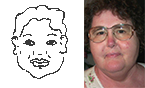
\includegraphics{111_2014_w_Kononova_face.png}
\end{center}

Программа, найдя на фотографии пациента похожее положение глаз, размер подбородка и др., выдаст нам результат о наличии или отсутствии травмы «Униженного». То же подходит и для других травм, только зависит от качества фотографий. Тело человека может содержать и несколько травм. Это потребует большего числа циклов обучения.

\subsubsection*{Вычисление диаграммы уровней мышления}

Согласно теории американского ученого К.~Грейвза, все живые системы в мире развиваются по спирали. По спирали также эволюционирует и мышление человека, приобретая четкие, характерные черты для каждого уровня мышления. Посредством онлайн теста можно построить для себя «диаграмму мышления» по типу jobEQ ASQ, ответив на некоторые вопросы:
\begin{center}
  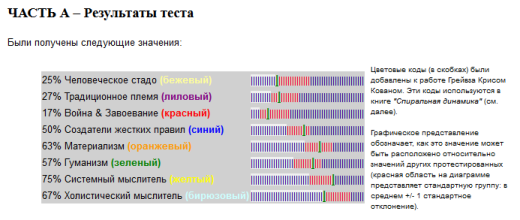
\includegraphics[width=\textwidth]{111_2014_w_Kononova_results.png}
	Осуществляется такой тест на свободном движке, например, testMaker 3.3.
\end{center}

\subsubsection*{Лаборатория экспериментов PEBL}

PEBL "--- Psychology Experiment Building Language. Это простой язык программирования для создания различных экспериментов на основе шаблонов. С помощью его реализации PEBL 0.13 можно запускать написанные на PEBL скрипты. Хорошей демонстрацией возможностей языка является скрипт, генерирующий случайные числа для выявления проблем с памятью.

\subsubsection*{Обработка звука в Audacity}

Для выведения человека из состояния шока широко используются специальные звуковые дорожки, в которых правильно подобраны частоты сигнала. С помощью Audacity легко подготовить звуковые дорожки, например для следующих целей:
\begin{itemize}
 \item	Устранение шумов и изоляция лишних звуков из многослойной дорожки, чтобы научить клиента фокусировать внимание на отдельных фракциях звука (обучение концентрации внимания).
 \item	Волны человеческого голоса имеют разную громкость на разном уровне частот. Разделив дорожку собственного голоса клиента на части, можно продемонстрировать ему, буквально «на каких частотах» он разговаривает в обычной жизни. Это позволит задуматься, что именно стоит изменить в поведении и общении.
 \item	Для активизации правого полушария мозга человека психологи часто применяют вдохновляющую музыку. Компиляции из нескольких композиций удобно делаются в Audacity простыми инструментами монтажа.
\end{itemize}

Поскольку большинство программ используется психологами для прикладных целей, то можно сделать вывод: свободное ПО даже на сегодняшний день предлагает весьма солидный инструментарий и совершенно не уступает собственническому ПО.
	Тем не менее, вопрос о разработке централизованного ПО для психологов и коучей, которое собрало бы в себя новые течения, было бы высококачественным и при этом свободным, остается на сегодняшний день открытым.

\subsection*{Краткий словарь:}

Коучинг "--- персональный систематический психологический тренинг, в рамках которого тренер путем совместного с клиентом поиска решений, обеспечивает улучшение качества жизни, самообучение и личностный рост клиента. (перевод определения Association for Coaching)

Архетип "--- (от греч. arche "--- начало и typos "--- образ) Прообраз, первоначальный образ, идея. Был введен К.\,Г.~Юнгом, как древнешие общечеловеческие символы, лежащие в основе мифов, фольклора и культуры. В данном контексте под архетипами подразумеваются совокупности поведенческих моделей, характерных для того или иного человека.

«Дизайн человека» "--- одна из современных психологических теорий, в основе которой лежит предположение, что момент рождения человека четко определяет возможные ветви его развития. Знание о конкретном моменте позволяет выстроить довольно сложную «карту» эволюции личности. Интересна тем, что было предпринято множество попыток автоматизировать процесс построения Дизайна человека.

\end{document}

\documentclass[10pt, a5paper]{article}
\usepackage{pdfpages}
\usepackage{parallel}
\usepackage[T2A]{fontenc}
\usepackage{ucs}
\usepackage[utf8x]{inputenc}
\usepackage[polish,english,russian]{babel}
\usepackage{hyperref}
\usepackage{rotating}
\usepackage[inner=2cm,top=1.8cm,outer=2cm,bottom=2.3cm,nohead]{geometry}
\usepackage{listings}
\usepackage{graphicx}
\usepackage{wrapfig}
\usepackage{longtable}
\usepackage{indentfirst}
\usepackage{array}
\newcolumntype{P}[1]{>{\raggedright\arraybackslash}p{#1}}
\frenchspacing
\usepackage{fixltx2e} %text sub- and superscripts
\usepackage{icomma} % коскі ў матэматычным рэжыме
\PreloadUnicodePage{4}

\newcommand{\longpage}{\enlargethispage{\baselineskip}}
\newcommand{\shortpage}{\enlargethispage{-\baselineskip}}

\def\switchlang#1{\expandafter\csname switchlang#1\endcsname}
\def\switchlangbe{
\let\saverefname=\refname%
\def\refname{Літаратура}%
\def\figurename{Іл.}%
}
\def\switchlangen{
\let\saverefname=\refname%
\def\refname{References}%
\def\figurename{Fig.}%
}
\def\switchlangru{
\let\saverefname=\refname%
\let\savefigurename=\figurename%
\def\refname{Литература}%
\def\figurename{Рис.}%
}

\hyphenation{admi-ni-stra-tive}
\hyphenation{ex-pe-ri-ence}
\hyphenation{fle-xi-bi-li-ty}
\hyphenation{Py-thon}
\hyphenation{ma-the-ma-ti-cal}
\hyphenation{re-ported}
\hyphenation{imp-le-menta-tions}
\hyphenation{pro-vides}
\hyphenation{en-gi-neering}
\hyphenation{com-pa-ti-bi-li-ty}
\hyphenation{im-pos-sible}
\hyphenation{desk-top}
\hyphenation{elec-tro-nic}
\hyphenation{com-pa-ny}
\hyphenation{de-ve-lop-ment}
\hyphenation{de-ve-loping}
\hyphenation{de-ve-lop}
\hyphenation{da-ta-ba-se}
\hyphenation{plat-forms}
\hyphenation{or-ga-ni-za-tion}
\hyphenation{pro-gramming}
\hyphenation{in-stru-ments}
\hyphenation{Li-nux}
\hyphenation{sour-ce}
\hyphenation{en-vi-ron-ment}
\hyphenation{Te-le-pathy}
\hyphenation{Li-nux-ov-ka}
\hyphenation{Open-BSD}
\hyphenation{Free-BSD}
\hyphenation{men-ti-on-ed}
\hyphenation{app-li-ca-tion}

\def\progref!#1!{\texttt{#1}}
\renewcommand{\arraystretch}{2} %Іначай формулы ў матрыцы зліпаюцца з лініямі
\usepackage{array}

\def\interview #1 (#2), #3, #4, #5\par{

\section[#1, #3, #4]{#1 -- #3, #4}
\def\qname{LVEE}
\def\aname{#1}
\def\q ##1\par{{\noindent \bf \qname: ##1 }\par}
\def\a{{\noindent \bf \aname: } \def\qname{L}\def\aname{#2}}
}

\def\interview* #1 (#2), #3, #4, #5\par{

\section*{#1\\{\small\rm #3, #4. #5}}

\def\qname{LVEE}
\def\aname{#1}
\def\q ##1\par{{\noindent \bf \qname: ##1 }\par}
\def\a{{\noindent \bf \aname: } \def\qname{L}\def\aname{#2}}
}

\begin{document}
\title{Обзор GNURadio}
\author{Юрий Адамов, Минск, Беларусь\footnote{\url{begemotv2718@tut.by}, \url{http://lvee.org/ru/abstracts/115}}}
\maketitle
\begin{abstract}
Gnuradio is a software framework intended in particular to building software defined radio. New functions and new external devices can be added easily by writing plugins. It also has graphical front end to rapidly create software signal processors.
I will demonstrate creating software radio receivers with GNUradio and commodity components.
Also I will discuss using gnuradio as a general signal processing tool and writing plugins for gnuradio, using processing of electroencephalogram (EEG) as an example.
\end{abstract}
\subsection*{От обычного радио к программно определяемому радио}

Изначально все компоненты радиоприемников и радиопередатчиков создавались из дискретных компонент. Из отдельных катушек, резисторов,  конденсаторов, транзисторов и т.п. собирались устройства, которые применяли определенные математические преобразования к исходному сигналу, принятому в антенне, дабы получить какой-то полезный сигнал на выходе. Например, типичный супергетеродинный приемник осуществляет предварительное усиление сигнала (умножение на константу в идеале), преобразование частоты (перемножение исходного сигнала и сигнала внутреннего генератора "--- гетеродина), фильтрацию получившегося сигнала полосовым фильтром, детектирование сигнала.

Возьмем более сложную систему "--- телевизор. Он также может быть описан как совокупность сравнительно простых блоков, осуществляющих простые математические преобразования сигнала: перенос телевизионного сигнала на промежуточную частоту (гетеродин "--- смеситель), усиление полного сигнала на промежуточной частоте (фильтр, усилитель), выделение несущих звука и изображения (фильтры), детектирование звука и изображения (AM детектор, FM детектор), усилители, выделение сигналов цветности (фильтры), детектирование сигналов цветности (FM детекторы), линии задержки (фазовый преобразователь), сумматоры (восстановление R,\,G,\,B), схемы синхронизации (пороговый детектор).

Несмотря на чисто аналоговую элементную базу, проектирование сложного радиоэлектронного прибора подобно проектированию программной системы "--- мы разбиваем систему на слабосвязанные функциональные блоки, блоки разбиваем на подблоки, пока не дойдем до элементарных операций (усиления, фильтрации, детектирования, порогового детектирования и т.д.).

Сейчас, когда частоты цифровой электроники уже довольно глубоко в радиодиапазоне, стало возможным сначала преобразовать сигнал из антенны в цифровую форму и затем делать многие из перечисленных выше операций уже на цифровых процессорах. При этом проектирование системы можно устраивать как средствами обычных языков программирования, так и с помощью старых добрых блок-схем.

Программно-определяемые радиосистемы, собственно, и предназначены для такой задачи. Gnuradio "--- как раз представитель подобного класса систем.

Рассмотрим чуть подробнее возможности современного процессора по обработке радиосигнала. Если мы возьмем диапазон длинных волн (30-300 кГц, километровые волны), то за один период этого сигнала успевает пройти более 10000 тактов процессора. Этого более чем достаточно, чтобы сделать с сигналом все что угодно (например, принять одновременно все длинноволновые станции и записывать каждую из них в отдельный файл). При этом процессор справится даже если мы добавим к ДВ существенный кусок средневолнового диапазона (300 кГц -- 3 МГц). Однако выполнить то же самое с наиболее интересными коротковолновым, УКВ и СВЧ диапазонами так просто не получится: в запасе остается слишком мало тактов. Здесь приходится использовать компромисс: с помощью аналоговой электроники часть представляющего интерес диапазона можно перенести по частоте в диапазон от 0 до нескольких мегагерц, а потом уже этот сигнал оцифровывать и обрабатывать с помощью программно-определяемого радио.

Практически те же самые средства, как программные так и аппаратные, работают и в обратную сторону "--- для подготовки к передаче сигнала в эфир.

Предварительное преобразование и оцифровку сигнала делает специальная аппаратура Universal software radio peripheral (USRP, универсальное внешнее устройство для программного радио). Она содержит в себе предварительный усилитель, преобразователь частоты и АЦП. До недавнего времени это были специализированные и потому сравнительно дорогие устройства (например, USRP фирмы Ettus research стоит порядка \textbackslash{}\$700). Однако несколько лет назад были открыты свойства USRP у сравнительно дешевых устройств для приема DVB-T телевидения на базе чипов Elonics E4000 и Raphael Micro R820T. Эти устройства стоят порядка \textbackslash{}\$20, имеют довольно широкий диапазон частот настройки (54---2200 МГц у E4000, 24---1700 МГц у R820T), большую частоту выборки АЦП (2.5 Ms/s) и приемлемую чувствительность. Недостатки таких приемников DVB-T "--- закрытость и невозможность передачи сигнала. Подобных недостатков лишен проект HackRF "--- свободное аппаратное обеспечение с возможностью приема и передачи. Однако, HackRF дороже и может вызвать претензии у служб радиоконтроля и таможни (поскольку является передатчиком).

\subsection*{Архитектура Gnuradio}

Все схемы в GNUradio строятся из \emph{блоков}. Блок "--- это элементарная единица обработки сигнала, «черный ящик» с несколькими входами и выходами. Выходы одних блоков можно соединять с однотипными входами других блоков, строя блок-схемы. Блоки можно соединять как программно (внутри программ на Python или C++) так и в графическом редакторе (GNURadio companion). Алгоритм обработки сигнала внутри блока реализуется на C++ (с ассемблерными вставками), для всех блоков существует обвязка на Python.

Блоки делятся на источники (sources), потребители (sinks), промежуточные и т.д. Также имеется большая библиотека графических виджетов, оформленных в виде блоков (поддерживаются Wx- и QT-виджеты).

Источники не имеют входов, зато имеют выходы. К источникам относятся интерфейсы USRP-приемников, программные генераторы сигналов, интерфейсы к микрофонам звуковой карточки, файлы с записями сигналов\ldots{} Например, описанные в предыдущем разделе приемники DVB-T  обрабатываются блоком RTL-SDR.

Потребители (sinks) не имеют выходов, но имеют один или несколько входов. К потребителям относят интерфейсы USRP-передатчиков, выходы звуковой карточки, выводы в файл. Некоторые графические виджеты также относятся к потребителям (например анализатор спектра, осциллограф).

Имеются потребители и источники, конвертирующие сигнал в/из TCP или UDP-поток данных. С помощью таких блоков можно разделить обработку сигнала на несколько машин.

Типичный представитель промежуточных блоков "--- фильтр. Имеется полный набор стандартных FIR или IIR-фильтров. Также фильтры могут конвертировать частоту выборки сигнала (децимация). Еще один класс промежуточных блоков "--- детекторы.

Имеются также вспомогательные блоки "--- например, представляющие глобальные переменные или виджеты для настройки глобальных переменных.

Для примера разберем, как сделать работающий FM-приемник из стандартных компонент GNUradio. Блок-схема самого простого приемника показана на рисунке.  Он состоит из источника (RTL-SDR), фильтра нижних частот (селектор сигнала одной станции), FM-детектора, еще ресэмплера и потребителя "--- аудиокарточки. Частота настройки и частота выборки задаются глобальными переменными. Для удобства работы добавим виджеты настройки и красивую картинку для спектра сигнала. Чтобы превратить эту схему в приемник AM-сигнала, достаточно заменить детектор. Можно устроить одновременный прием двух FM станций, если они помещаются в полосу частот 1 MГц. Для этого можно использовать блок сдвига частоты frequency XLATE.

\begin{center}
  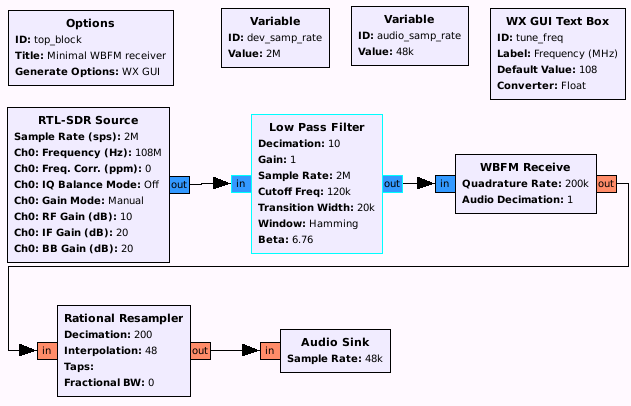
\includegraphics[width=\textwidth]{112_2014_w_Adamov_struct.png}
\end{center}

\subsection*{Нестандартные применения GNUradio и написание своих блоков}

Хотя проект GNUradio изначально предназначен для задач обработки радиосигналов, он предоставляет набор стандартных хорошо оптимизированных компонент, пригодных для любой цифровой обработки сигналов. В качестве еще одного примера рассмотрим, как можно обработать данные энцефалограммы человека (запись мозговой активности). Для анализа в энцефалограмме выделяют несколько ритмов, они лежат в разных диапазонах частот (альфа 8---13 Гц, бета 13---30 Гц, гамма \textgreater{} 30 Гц, тета и дельта 1---7 Гц). Для определения активности в этих каналах нужно отфильтровать соответствующие диапазоны частот, по возможности сдвинуть частоты к нулю, продетектировать и усреднить сигнал. Однако данные от энцефалографа поступают в виде csv-файла, который стандартные средства GNUradio читать не умеют. С помощью gr\_modtool мы создаем шаблон нового компонента

\verb!% gr_modtool newmod csvfile!

Добавляем источник с типом выходных данных float (f).

\verb!% cd gr_csvfile!

\verb!% gr_modtool add -t source csvfile_f!

Это создает структуру директорий:

\verb!% ls gr_csvfile!

\verb!apps cmake CMakeLists.txt docs examples!

\verb!grc include lib python swig!

Нам в первую очередь потребуется отредактировать файлы \textbf{сsv\-file\_f\_impl.cc} и \textbf{csvfile\_f\_impl.h}. В качестве образца возьмем стандартный компонент чтения из wav-файла, который есть в исходных кодах GNUradio. Нужно также отредактировать xml-файл описания компонента в директории grc. Далее, после компиляции с помощью cmake, получаем нужный компонент.

\end{document}

%\input{101_2014_w_LastName}
%\documentclass[10pt, a5paper]{article}
\usepackage{pdfpages}
\usepackage{parallel}
\usepackage[T2A]{fontenc}
\usepackage{ucs}
\usepackage[utf8x]{inputenc}
\usepackage[polish,english,russian]{babel}
\usepackage{hyperref}
\usepackage{rotating}
\usepackage[inner=2cm,top=1.8cm,outer=2cm,bottom=2.3cm,nohead]{geometry}
\usepackage{listings}
\usepackage{graphicx}
\usepackage{wrapfig}
\usepackage{longtable}
\usepackage{indentfirst}
\usepackage{array}
\newcolumntype{P}[1]{>{\raggedright\arraybackslash}p{#1}}
\frenchspacing
\usepackage{fixltx2e} %text sub- and superscripts
\usepackage{icomma} % коскі ў матэматычным рэжыме
\PreloadUnicodePage{4}

\newcommand{\longpage}{\enlargethispage{\baselineskip}}
\newcommand{\shortpage}{\enlargethispage{-\baselineskip}}

\def\switchlang#1{\expandafter\csname switchlang#1\endcsname}
\def\switchlangbe{
\let\saverefname=\refname%
\def\refname{Літаратура}%
\def\figurename{Іл.}%
}
\def\switchlangen{
\let\saverefname=\refname%
\def\refname{References}%
\def\figurename{Fig.}%
}
\def\switchlangru{
\let\saverefname=\refname%
\let\savefigurename=\figurename%
\def\refname{Литература}%
\def\figurename{Рис.}%
}

\hyphenation{admi-ni-stra-tive}
\hyphenation{ex-pe-ri-ence}
\hyphenation{fle-xi-bi-li-ty}
\hyphenation{Py-thon}
\hyphenation{ma-the-ma-ti-cal}
\hyphenation{re-ported}
\hyphenation{imp-le-menta-tions}
\hyphenation{pro-vides}
\hyphenation{en-gi-neering}
\hyphenation{com-pa-ti-bi-li-ty}
\hyphenation{im-pos-sible}
\hyphenation{desk-top}
\hyphenation{elec-tro-nic}
\hyphenation{com-pa-ny}
\hyphenation{de-ve-lop-ment}
\hyphenation{de-ve-loping}
\hyphenation{de-ve-lop}
\hyphenation{da-ta-ba-se}
\hyphenation{plat-forms}
\hyphenation{or-ga-ni-za-tion}
\hyphenation{pro-gramming}
\hyphenation{in-stru-ments}
\hyphenation{Li-nux}
\hyphenation{sour-ce}
\hyphenation{en-vi-ron-ment}
\hyphenation{Te-le-pathy}
\hyphenation{Li-nux-ov-ka}
\hyphenation{Open-BSD}
\hyphenation{Free-BSD}
\hyphenation{men-ti-on-ed}
\hyphenation{app-li-ca-tion}

\def\progref!#1!{\texttt{#1}}
\renewcommand{\arraystretch}{2} %Іначай формулы ў матрыцы зліпаюцца з лініямі
\usepackage{array}

\def\interview #1 (#2), #3, #4, #5\par{

\section[#1, #3, #4]{#1 -- #3, #4}
\def\qname{LVEE}
\def\aname{#1}
\def\q ##1\par{{\noindent \bf \qname: ##1 }\par}
\def\a{{\noindent \bf \aname: } \def\qname{L}\def\aname{#2}}
}

\def\interview* #1 (#2), #3, #4, #5\par{

\section*{#1\\{\small\rm #3, #4. #5}}

\def\qname{LVEE}
\def\aname{#1}
\def\q ##1\par{{\noindent \bf \qname: ##1 }\par}
\def\a{{\noindent \bf \aname: } \def\qname{L}\def\aname{#2}}
}

\begin{document}
\title{Голос спонсора: SaM Solutions}
%\author{}
\date{}
\maketitle

Компания SaM Solutions выступает в роли системо-образующего спонсора конференции Linux Vacation Eastern Europe с момента рождения LVEE в 2005 году и на протяжении всех лет её проведения. 

Сложившаяся корпоративная практика не случайна. Продукты и решения, задействующие Linux и другие Free/Open Source Software проекты, составляют заметную часть пакета разработок SaM Solutions. Кадровая политика компании направлена на поощрение профессионального развития своих сотрудников, организацию их эффективного отдыха и привлечение хорошо мотивированных кандидатов к работе на компанию. Формат конференции LVEE успешно позволяет решать все три задачи. 

Одним из подразделений компании является отдел Linux и \linebreak Embbeded. Специалисты компании на протяжении десятилетий работают с СПО. Компанией реализован ряд проектов по адаптации ОС GNU/Linux для работы в различных устройствах, построенных на таких платформах как ARM, PowerPC, x86, MIPS. В последние годы "--- на ведущие позиции выходит разработка управляющего ПО для серверов Enterprise-класса, от низкоуровнего BMC Firmware на основе Linux до высокоуровневых систем контроля виртуализации и графических интерфейсов управления, от прошивок устройств хранения данных до BSP интегрированных плат для разработчика. Надёжность, качество и широкая функциональность множества свободных проектов позволяет строить нам системы любого уровня и сложности, опираясь на высококачественные готовые компоненты.

В рамках направления Linux и Embedded успешно выполнены проекты для таких знаковых заказчиков, как  Novell/SUSE, Fujitsu Technology Solutions  и осуществляется партнёрство с компаниями IBM и Oracle/Sun в области Open Source решений.

Мы разрабатываем, модифицируем и адаптируем различное свободное программное обеспечение для наших заказчиков, но не забываем и о своих нуждах "--- наши сотрудники используют в своей работе существующие програмные продукты и вносят вклад в их развитие. Часть внутренней инфраструктуры, а именно интранет-сеть компании, тестовые стенды отдела контроля качества, рабочие места сотрудников профильных подразделений "--- также работает под управлением СПО (серверные и десктопные платформы GNU/Linux и FreeBSD). 

В минувшем году, в рамках реорганизации, был разработан долгосрочный план развития направления Linux и Embedded в SaM Solutions. В нём впервые были кодифицированы уже имеющиеся внутренние неофициальные практики по взаимодействию с commu"=nity-based проектами. В частности разработаны меры и правила по
\begin{itemize}
  \item возврата изменений в родительские проекты (upstreaming);
  \item вхождения в состав постоянных разработчиков активно используемых нами FOSS-компонентов;
  \item публикации сообщений об ошибках (bug reporting);
  \item участия и помощи в организации community events;
  \item стимуляции докладов и участия в технических конференциях.
\end{itemize}
И план немедленно начал претворяться в жизнь.

Силами отдела организовано внутреннее обучение сотрудников на регулярной
основе. Был прочтен и опубликован курс по TDD. По согласованию с автором
опубликован курс Debian/Ubuntu Packaging (видео, презентация и исходные
тексты презентации в \LaTeX).  Были организованы и проведены курсы по
обучению QA специалистов для направления Embeded Linux. Проведено
практическое занятие по основам виртуализации и эмуляции, организована
лекция по вопросу профилирования и оптимизации Ruby-кода, лекция о
High-availability кластерах и направлении развития технологии. Кроме того,
проводился семинар по Video4Linux2. Для создания и обучения кадрового
резерва на ближайшее будущее запланированы постоянно действующие внутренние
проекты в области Embedded Linux, результаты которых также запланированы к
публикации.

Визиты представительных делегаций на Embedded World 2012 и Linux Con Europe/Embedded LinuxCon Europe 2011 обогатили нас новыми идеями, куда можно
двигаться дальше и что сейчас актуально. А выступления на Software
Engineering Forum for Students, круглом столе по СПО в рамках TIBO-2012
и LVEE Winter 2012 позволили поделиться опытом с
заинтересованными сторонами.

В апреле состоялась Ганноверская промышленная ярмарка \linebreak (Hannover Messe
2013). Компания SaM Solutions была представлена отдельным стендом, на
котором демонстрировались наработки в области встроенного и системного ПО
на базе OS Linux. Идея «умного» дома вызвала неподдельный интерес у
посетителей стенда.

При поддержке SaM Solutions, с декабря 2011 года возобновились регулярные встречи Minsk Linux Users Groups, под названием <<Линуксовка в SaM Solutions>>. Техническое оснащение линуксовок и открытый формат встреч позволил им практически мгновенно стать заметным дискуссионным клубом по широкому спектру вопросов, прямо или косвенно связанных с СПО. Свободная картография (OpenStreetMap), технологии виртуализации, минский \linebreak hackerspace, Linux Mobile, бойкот Голливудской продукции, systemd, загрузчик u-boot, белорусская локализация GNOME --- это только часть тем, поднятых за последние линуксовки.

Быстрые и положительные изменения, как внутри компании SaM Solutions, так и в экосфере СПО (и Linux в частности) наполняют нас уверенностью, что направление движения выбрано верно.

\begin{figure}[h!]
\centering
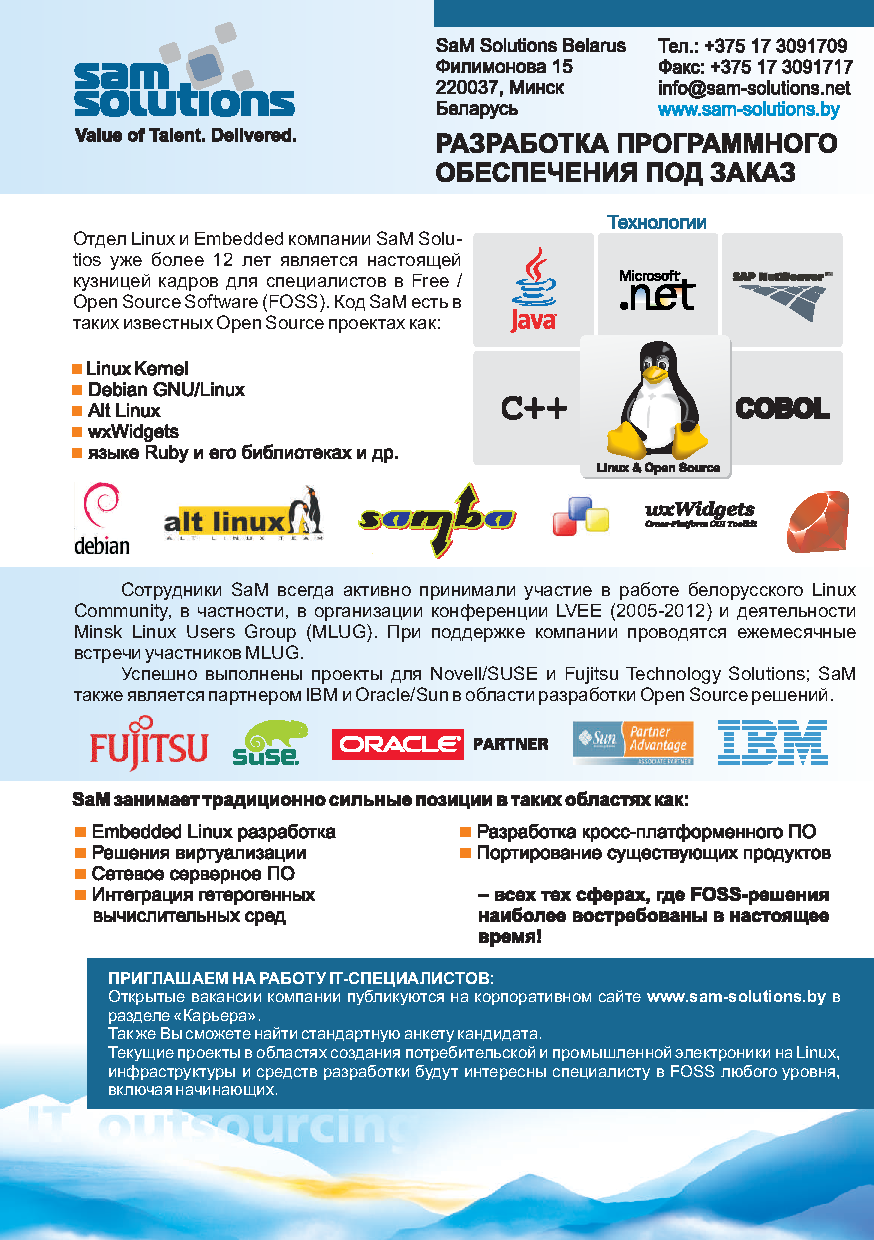
\includegraphics[height=11.8cm]{48_spons_sams.pdf}
\end{figure}
\end{document}



%\documentclass[10pt, a5paper]{article}
\usepackage{pdfpages}
\usepackage{parallel}
\usepackage[T2A]{fontenc}
\usepackage{ucs}
\usepackage[utf8x]{inputenc}
\usepackage[polish,english,russian]{babel}
\usepackage{hyperref}
\usepackage{rotating}
\usepackage[inner=2cm,top=1.8cm,outer=2cm,bottom=2.3cm,nohead]{geometry}
\usepackage{listings}
\usepackage{graphicx}
\usepackage{wrapfig}
\usepackage{longtable}
\usepackage{indentfirst}
\usepackage{array}
\newcolumntype{P}[1]{>{\raggedright\arraybackslash}p{#1}}
\frenchspacing
\usepackage{fixltx2e} %text sub- and superscripts
\usepackage{icomma} % коскі ў матэматычным рэжыме
\PreloadUnicodePage{4}

\newcommand{\longpage}{\enlargethispage{\baselineskip}}
\newcommand{\shortpage}{\enlargethispage{-\baselineskip}}

\def\switchlang#1{\expandafter\csname switchlang#1\endcsname}
\def\switchlangbe{
\let\saverefname=\refname%
\def\refname{Літаратура}%
\def\figurename{Іл.}%
}
\def\switchlangen{
\let\saverefname=\refname%
\def\refname{References}%
\def\figurename{Fig.}%
}
\def\switchlangru{
\let\saverefname=\refname%
\let\savefigurename=\figurename%
\def\refname{Литература}%
\def\figurename{Рис.}%
}

\hyphenation{admi-ni-stra-tive}
\hyphenation{ex-pe-ri-ence}
\hyphenation{fle-xi-bi-li-ty}
\hyphenation{Py-thon}
\hyphenation{ma-the-ma-ti-cal}
\hyphenation{re-ported}
\hyphenation{imp-le-menta-tions}
\hyphenation{pro-vides}
\hyphenation{en-gi-neering}
\hyphenation{com-pa-ti-bi-li-ty}
\hyphenation{im-pos-sible}
\hyphenation{desk-top}
\hyphenation{elec-tro-nic}
\hyphenation{com-pa-ny}
\hyphenation{de-ve-lop-ment}
\hyphenation{de-ve-loping}
\hyphenation{de-ve-lop}
\hyphenation{da-ta-ba-se}
\hyphenation{plat-forms}
\hyphenation{or-ga-ni-za-tion}
\hyphenation{pro-gramming}
\hyphenation{in-stru-ments}
\hyphenation{Li-nux}
\hyphenation{sour-ce}
\hyphenation{en-vi-ron-ment}
\hyphenation{Te-le-pathy}
\hyphenation{Li-nux-ov-ka}
\hyphenation{Open-BSD}
\hyphenation{Free-BSD}
\hyphenation{men-ti-on-ed}
\hyphenation{app-li-ca-tion}

\def\progref!#1!{\texttt{#1}}
\renewcommand{\arraystretch}{2} %Іначай формулы ў матрыцы зліпаюцца з лініямі
\usepackage{array}

\def\interview #1 (#2), #3, #4, #5\par{

\section[#1, #3, #4]{#1 -- #3, #4}
\def\qname{LVEE}
\def\aname{#1}
\def\q ##1\par{{\noindent \bf \qname: ##1 }\par}
\def\a{{\noindent \bf \aname: } \def\qname{L}\def\aname{#2}}
}

\def\interview* #1 (#2), #3, #4, #5\par{

\section*{#1\\{\small\rm #3, #4. #5}}

\def\qname{LVEE}
\def\aname{#1}
\def\q ##1\par{{\noindent \bf \qname: ##1 }\par}
\def\a{{\noindent \bf \aname: } \def\qname{L}\def\aname{#2}}
}

\begin{document}
\title{Голос спонсора: EPAM Systems}
%\author{}
\date{}
\maketitle

Компания EPAM Systems не первый год является спонсором международной конференции разработчиков и пользователей свободного программного обеспечения LVEE (Linux Vacation / Eastern Europe). Этот год также не стал исключением. Пожалуй, LVEE является самым значимым событием для русскоязычных разработчиков и тестировщиков Open Source. Каждое лето здесь встречаются начинающие специалисты и «ветераны»"=разработчики из десятка стран для обмена опытом и общения на профессиональные темы. Наши специалисты также активно участвуют в данной конференции: в качестве докладчиков и организаторов/волонтёров. Это уникальная в своём роде конференция, и именно поэтому EPAM Systems очередной раз принимает участие в LVEE в качестве спонсора.


EPAM Systems "--- одна из крупнейших компаний"=поставщиков\linebreak услуг в области разработки программного обеспечения и решений на территории СНГ и Центральной и Восточной Европы. Созданная в 1993 году, сегодня она имеет представительства в 12 странах мира, в штате работают более 9 тыс. сотрудников, из которых более 3 тыс. "--- в Беларуси. Рост компании обеспечивается за счет собственных обучающих программ и передаче опыта от больших специалистов до начинающих разработчиков. Компания EPAM Systems выполняет проекты более чем в 30 странах мира. Основные направления деятельности: разработка, тестирование, сопровождение и поддержка заказного программного обеспечения и бизнес"=приложений, а также ИТ"=консалтинг с учетом отраслевой специфики бизнеса.

Наша компания участвует в проектах с такими крупными, хорошо известными заказчиками как Google, Novell, Infoblox, Parallels, 10Gen и др., так и с небольшими, в том числе и с начинающими свой путь в софтверном бизнесе.


К примеру, для Infoblox была реализована связка между WebUI с BIND и DHCP. Для этого был разработан комплекс решений под управлением Shell и Python скриптов, а также механизм позволяющий вносить правки в BIND и DHCP на языке C. Также был разработан развернутый функционал, автоматизирующий инсталляцию новых устройств и их эксплуатацию, что позволяет значительно упростить управление данными. Встроенный Web"=интерфейс позволяет разворачивать, управлять сервисами DNS, DNSSEC, DHCP, IPAM, устанавливать новые версии ПО, архивировать и восстанавливать из архивов необходимые данные, восстанавливать их после аварии, проводить мониторинг сети и создавать отчеты без необходимости обращения к командной строке.


Еще одним решением, реализованным для компании Infoblox, являлся программный продукт, позволяющий контролировать сетевые изменения, таким образом, облегчая идентификацию трудноуловимых проблем конфигурации и соответствие требованиям. Вместо того чтобы просто регистрировать изменения, система использует внесенную информацию для проверки, анализа и автоматической обработки сетевых изменений. Благодаря инновационной, квалифицированной, глубокой технике логического анализа, программа изолирует проблемы исправности и конфигурации до того, как они могут вызвать более серьезные сбои.


Разработанная для анализа сложных сетей система изучает сеть, собирает ключевую информацию, применяет встроенную технику логического анализа и создает оценку исправности сети и список проблем, требующих принятие мер для улучшения качества работы сети.


Правильное использование свободного ПО в разработках сокращает и расходы на покупку лицензионных программ, и трудозатраты при создании коммерческого ПО. Немалую роль для достижения превосходного результата играет привлечение к разработке опытных специалистов. LVEE способствует появлению таких специалистов, развитию их навыков и расширению кругозора. Хотелось бы пожелать участникам конференции интересных проектов и максимум пользы от участия в LVEE.


\end{document}



%\documentclass[10pt, a5paper]{article}
\usepackage{pdfpages}
\usepackage{parallel}
\usepackage[T2A]{fontenc}
\usepackage{ucs}
\usepackage[utf8x]{inputenc}
\usepackage[polish,english,russian]{babel}
\usepackage{hyperref}
\usepackage{rotating}
\usepackage[inner=2cm,top=1.8cm,outer=2cm,bottom=2.3cm,nohead]{geometry}
\usepackage{listings}
\usepackage{graphicx}
\usepackage{wrapfig}
\usepackage{longtable}
\usepackage{indentfirst}
\usepackage{array}
\newcolumntype{P}[1]{>{\raggedright\arraybackslash}p{#1}}
\frenchspacing
\usepackage{fixltx2e} %text sub- and superscripts
\usepackage{icomma} % коскі ў матэматычным рэжыме
\PreloadUnicodePage{4}

\newcommand{\longpage}{\enlargethispage{\baselineskip}}
\newcommand{\shortpage}{\enlargethispage{-\baselineskip}}

\def\switchlang#1{\expandafter\csname switchlang#1\endcsname}
\def\switchlangbe{
\let\saverefname=\refname%
\def\refname{Літаратура}%
\def\figurename{Іл.}%
}
\def\switchlangen{
\let\saverefname=\refname%
\def\refname{References}%
\def\figurename{Fig.}%
}
\def\switchlangru{
\let\saverefname=\refname%
\let\savefigurename=\figurename%
\def\refname{Литература}%
\def\figurename{Рис.}%
}

\hyphenation{admi-ni-stra-tive}
\hyphenation{ex-pe-ri-ence}
\hyphenation{fle-xi-bi-li-ty}
\hyphenation{Py-thon}
\hyphenation{ma-the-ma-ti-cal}
\hyphenation{re-ported}
\hyphenation{imp-le-menta-tions}
\hyphenation{pro-vides}
\hyphenation{en-gi-neering}
\hyphenation{com-pa-ti-bi-li-ty}
\hyphenation{im-pos-sible}
\hyphenation{desk-top}
\hyphenation{elec-tro-nic}
\hyphenation{com-pa-ny}
\hyphenation{de-ve-lop-ment}
\hyphenation{de-ve-loping}
\hyphenation{de-ve-lop}
\hyphenation{da-ta-ba-se}
\hyphenation{plat-forms}
\hyphenation{or-ga-ni-za-tion}
\hyphenation{pro-gramming}
\hyphenation{in-stru-ments}
\hyphenation{Li-nux}
\hyphenation{sour-ce}
\hyphenation{en-vi-ron-ment}
\hyphenation{Te-le-pathy}
\hyphenation{Li-nux-ov-ka}
\hyphenation{Open-BSD}
\hyphenation{Free-BSD}
\hyphenation{men-ti-on-ed}
\hyphenation{app-li-ca-tion}

\def\progref!#1!{\texttt{#1}}
\renewcommand{\arraystretch}{2} %Іначай формулы ў матрыцы зліпаюцца з лініямі
\usepackage{array}

\def\interview #1 (#2), #3, #4, #5\par{

\section[#1, #3, #4]{#1 -- #3, #4}
\def\qname{LVEE}
\def\aname{#1}
\def\q ##1\par{{\noindent \bf \qname: ##1 }\par}
\def\a{{\noindent \bf \aname: } \def\qname{L}\def\aname{#2}}
}

\def\interview* #1 (#2), #3, #4, #5\par{

\section*{#1\\{\small\rm #3, #4. #5}}

\def\qname{LVEE}
\def\aname{#1}
\def\q ##1\par{{\noindent \bf \qname: ##1 }\par}
\def\a{{\noindent \bf \aname: } \def\qname{L}\def\aname{#2}}
}

%\frenchspacing
\begin{document}
\title{Голос спонсора: ITS Partner}
%\author{}
\date{}
\maketitle%

~

\end{document}



%\documentclass[10pt, a5paper]{article}
\usepackage{pdfpages}
\usepackage{parallel}
\usepackage[T2A]{fontenc}
\usepackage{ucs}
\usepackage[utf8x]{inputenc}
\usepackage[polish,english,russian]{babel}
\usepackage{hyperref}
\usepackage{rotating}
\usepackage[inner=2cm,top=1.8cm,outer=2cm,bottom=2.3cm,nohead]{geometry}
\usepackage{listings}
\usepackage{graphicx}
\usepackage{wrapfig}
\usepackage{longtable}
\usepackage{indentfirst}
\usepackage{array}
\newcolumntype{P}[1]{>{\raggedright\arraybackslash}p{#1}}
\frenchspacing
\usepackage{fixltx2e} %text sub- and superscripts
\usepackage{icomma} % коскі ў матэматычным рэжыме
\PreloadUnicodePage{4}

\newcommand{\longpage}{\enlargethispage{\baselineskip}}
\newcommand{\shortpage}{\enlargethispage{-\baselineskip}}

\def\switchlang#1{\expandafter\csname switchlang#1\endcsname}
\def\switchlangbe{
\let\saverefname=\refname%
\def\refname{Літаратура}%
\def\figurename{Іл.}%
}
\def\switchlangen{
\let\saverefname=\refname%
\def\refname{References}%
\def\figurename{Fig.}%
}
\def\switchlangru{
\let\saverefname=\refname%
\let\savefigurename=\figurename%
\def\refname{Литература}%
\def\figurename{Рис.}%
}

\hyphenation{admi-ni-stra-tive}
\hyphenation{ex-pe-ri-ence}
\hyphenation{fle-xi-bi-li-ty}
\hyphenation{Py-thon}
\hyphenation{ma-the-ma-ti-cal}
\hyphenation{re-ported}
\hyphenation{imp-le-menta-tions}
\hyphenation{pro-vides}
\hyphenation{en-gi-neering}
\hyphenation{com-pa-ti-bi-li-ty}
\hyphenation{im-pos-sible}
\hyphenation{desk-top}
\hyphenation{elec-tro-nic}
\hyphenation{com-pa-ny}
\hyphenation{de-ve-lop-ment}
\hyphenation{de-ve-loping}
\hyphenation{de-ve-lop}
\hyphenation{da-ta-ba-se}
\hyphenation{plat-forms}
\hyphenation{or-ga-ni-za-tion}
\hyphenation{pro-gramming}
\hyphenation{in-stru-ments}
\hyphenation{Li-nux}
\hyphenation{sour-ce}
\hyphenation{en-vi-ron-ment}
\hyphenation{Te-le-pathy}
\hyphenation{Li-nux-ov-ka}
\hyphenation{Open-BSD}
\hyphenation{Free-BSD}
\hyphenation{men-ti-on-ed}
\hyphenation{app-li-ca-tion}

\def\progref!#1!{\texttt{#1}}
\renewcommand{\arraystretch}{2} %Іначай формулы ў матрыцы зліпаюцца з лініямі
\usepackage{array}

\def\interview #1 (#2), #3, #4, #5\par{

\section[#1, #3, #4]{#1 -- #3, #4}
\def\qname{LVEE}
\def\aname{#1}
\def\q ##1\par{{\noindent \bf \qname: ##1 }\par}
\def\a{{\noindent \bf \aname: } \def\qname{L}\def\aname{#2}}
}

\def\interview* #1 (#2), #3, #4, #5\par{

\section*{#1\\{\small\rm #3, #4. #5}}

\def\qname{LVEE}
\def\aname{#1}
\def\q ##1\par{{\noindent \bf \qname: ##1 }\par}
\def\a{{\noindent \bf \aname: } \def\qname{L}\def\aname{#2}}
}

\begin{document}
\title{Голос спонсора: Promwad}
%\author{}
\date{}
\maketitle
%\begin{wrapfigure}{l}{0.3\textwidth}

\begin{figure}[h!]
\centering

\includegraphics[width=10cm]{53_spons_promwad.png}
\end{figure}

{\bf Инновационная компания Promwad} реализует полный цикл разработки электроники: создание концепции продукта, промышленный дизайн и конструирование, проектирование аппаратных \linebreak платформ, разработка встроенного и прикладного ПО, тестирование ПО и контроль качества, сертификация, изготовление опытных образцов, постановка и сопровождение массового производства.

Promwad предлагает услуги аутсорсинга разработки электронных устройств в различных отраслях рынка электроники: телекоммуникации, автомобильная электроника, автоматизация, потребительская электроника, медиа и развлечения и другие. 

Разработка встроенного ПО "--- одна из основных услуг и направлений развития Promwad. Мы разрабатываем ПО для микропроцессоров, систем-на-кристалле, цифровых сигнальных процессоров и микроконтроллеров.

Наши разработчики работают с:
\begin{itemize}
\item Операционными системами "--- GNU/Linux, Android, FreeRTOS, RTEMS и другие специализированные RTOS
\item Языками программирования "--- C (user-space, kernel-space),\linebreak ARM Assembler, C++, Unix shell, Lua, Python, Javascript
\item Графическими библиотеками "--- QT+QML, SDL, OpenGL
\item Linux подсистемами "--- network drivers, USB, PCI, UART, SPI, I2C, GPIO, IRQs, Real time scheduling, cryptography, DMA, PMIC, ALSA, touchscreen, sensors, framebuffer, v4l2
\item Базами данных "--- MySQL, sqlite
\item Средствами сборки "--- make, Automake/Autotools, Cmake, \linebreak Qmak
\item Сборочными системами, фреймворками "--- Buildroot, \linebreak OpenEmbedded, Yocto, Openwrt, rpm/rpmbuild, deb/debuild, uClinux, STAPI
\item Отладками "--- jtag, openocd, valgrind, gdb
\item Системами контроля версий "--- SVN, GIT
\end{itemize}

В компании всегда открыт набор специалистов- разработчиков Linux Embedded, имеющих опыт работы  на языке программирования С/С++  в сфере Embedded не менее двух лет.

Сегодня Promwad "--- это успешная компания на рынке электроники и IT, резидент Парка высоких технологий (ПВТ), участник партнерских программ ведущих мировых производителей электронных компонентов, таких как Texas Instruments, STMicroelectronics, Analog Devices, Marvell и Fujitsu. 

Как современная компания мы уделяем внимание внутренним ценностям: обучение, развитие сотрудников, активный отдых, спонсорство и участие в тематических конференциях и тп. (с 2007 года Promwad постоянный спонсор конференций LVEE, а с 2009 года проводит собственный Форум разработчиков цифровой электроники "--- DEDF).

Как социально ответственная компания мы являемся партнером и титульным спонсором Кубка приключенческих гонок "--- ПромвадТур, который объединяет неравнодушных к активному досугу и приключениям единомышленников различных профессий. 

Описание услуг  компании, портфолио выполненных проектов, текущие вакансии и другую полезную информацию смотрите на корпоративном сайте Promwad: \url{www.promwad.com}.

{\bf Мы любим то, что делаем, и работаем на результат! Если ты разделяешь нашу позицию "--- будем рады принять в команду!}

%\documentclass[10pt, a5paper]{article}
\usepackage{pdfpages}
\usepackage{parallel}
\usepackage[T2A]{fontenc}
\usepackage{ucs}
\usepackage[utf8x]{inputenc}
\usepackage[polish,english,russian]{babel}
\usepackage{hyperref}
\usepackage{rotating}
\usepackage[inner=2cm,top=1.8cm,outer=2cm,bottom=2.3cm,nohead]{geometry}
\usepackage{listings}
\usepackage{graphicx}
\usepackage{wrapfig}
\usepackage{longtable}
\usepackage{indentfirst}
\usepackage{array}
\newcolumntype{P}[1]{>{\raggedright\arraybackslash}p{#1}}
\frenchspacing
\usepackage{fixltx2e} %text sub- and superscripts
\usepackage{icomma} % коскі ў матэматычным рэжыме
\PreloadUnicodePage{4}

\newcommand{\longpage}{\enlargethispage{\baselineskip}}
\newcommand{\shortpage}{\enlargethispage{-\baselineskip}}

\def\switchlang#1{\expandafter\csname switchlang#1\endcsname}
\def\switchlangbe{
\let\saverefname=\refname%
\def\refname{Літаратура}%
\def\figurename{Іл.}%
}
\def\switchlangen{
\let\saverefname=\refname%
\def\refname{References}%
\def\figurename{Fig.}%
}
\def\switchlangru{
\let\saverefname=\refname%
\let\savefigurename=\figurename%
\def\refname{Литература}%
\def\figurename{Рис.}%
}

\hyphenation{admi-ni-stra-tive}
\hyphenation{ex-pe-ri-ence}
\hyphenation{fle-xi-bi-li-ty}
\hyphenation{Py-thon}
\hyphenation{ma-the-ma-ti-cal}
\hyphenation{re-ported}
\hyphenation{imp-le-menta-tions}
\hyphenation{pro-vides}
\hyphenation{en-gi-neering}
\hyphenation{com-pa-ti-bi-li-ty}
\hyphenation{im-pos-sible}
\hyphenation{desk-top}
\hyphenation{elec-tro-nic}
\hyphenation{com-pa-ny}
\hyphenation{de-ve-lop-ment}
\hyphenation{de-ve-loping}
\hyphenation{de-ve-lop}
\hyphenation{da-ta-ba-se}
\hyphenation{plat-forms}
\hyphenation{or-ga-ni-za-tion}
\hyphenation{pro-gramming}
\hyphenation{in-stru-ments}
\hyphenation{Li-nux}
\hyphenation{sour-ce}
\hyphenation{en-vi-ron-ment}
\hyphenation{Te-le-pathy}
\hyphenation{Li-nux-ov-ka}
\hyphenation{Open-BSD}
\hyphenation{Free-BSD}
\hyphenation{men-ti-on-ed}
\hyphenation{app-li-ca-tion}

\def\progref!#1!{\texttt{#1}}
\renewcommand{\arraystretch}{2} %Іначай формулы ў матрыцы зліпаюцца з лініямі
\usepackage{array}

\def\interview #1 (#2), #3, #4, #5\par{

\section[#1, #3, #4]{#1 -- #3, #4}
\def\qname{LVEE}
\def\aname{#1}
\def\q ##1\par{{\noindent \bf \qname: ##1 }\par}
\def\a{{\noindent \bf \aname: } \def\qname{L}\def\aname{#2}}
}

\def\interview* #1 (#2), #3, #4, #5\par{

\section*{#1\\{\small\rm #3, #4. #5}}

\def\qname{LVEE}
\def\aname{#1}
\def\q ##1\par{{\noindent \bf \qname: ##1 }\par}
\def\a{{\noindent \bf \aname: } \def\qname{L}\def\aname{#2}}
}

\begin{document}
\title{Голос спонсора: World of Tanks team}
%\author{}
\date{}
\maketitle

\subsection*{О проекте}

World of Tanks (Мир танков) "--- первый ММО проект ААА класса, созданный
белоруской командой. Разработчиками игра позиционируется как MMO"=экшн с
элементами ролевой игры, шутера и стратегии. Концепция <<World of Tanks>>
базируется на массовых командных танковых сражениях в режиме PvP. Онлайн
релиз русской версии игры состоялся 12 августа 2010 года, в марте 2011 года
состоялся <<китайский>> релиз, а в апреле 2011 года проект успешно вышел на
территории США и Европы.

Успех проекта World of Tanks можно оценить по целому ряду показателей:
количество активных игроков более 2 миллионов, рекордная цифра одновременной
игры "--- более 150.000 игроков на российском игровом кластере! В книгу
рекордов Гиннеса мы вошли 23 января 2011 года с показателем 91 311 игроков
он"=лайн. 

Дважды подряд в 2010 и 2011 году на Конференции Разработчиков Компьютерных
Игр (Москва) наш проект был признан Лучшей клиентской он"=лайн игрой (КРИ
2010) и Лучшей игрой (КРИ 2011).

В 2010 году по результатам международной выставки E3 (Лос"=Анжелес)
крупнейший ММО"=портал Massivly назвал наш проект New Concept 2010. В
настоящий момент определяются победители E3 2011. Мы сможем рассказать о
наших успехах уже при личной встрече на конференции LVEE 2011.

\subsection*{Подробности о проекте}

Игровые кластеры проекта находятся в дата"=центрах России, Германии, США и
Китая. Общее количество серверов в настоящий момент порядка 500, к концу
года мы планируем удвоить их количество.

Как игровые, так и прочие инфраструктурные сервера функционируют на базе
операционной системы CentOS.

Осенью 2010 года пики онлайна на российском игровом кластере достигали 30
тыс. В настоящий момент за счет высокотехнологичных решений наших
специалистов (включающих в себя оптимизацию сетевой инфраструктуры,
оптимизацию работы с базами данных, оптимизацию нашего серверного ПО) пик
он-лайна вырос до 150 тыс.

Высокая производительность достигается в т.~ч. за счет использования
free and open source software  как технологической основы для работы
серверной части самой масштабной ММО"=игры, а именно: CentOS,
MySQL, nginx, zabbix, nagios, cacti, python, django и т.~д.

\subsection*{О нас}

Над созданием проекта работает СООО <<Гейм Стрим>> "--- основной центр разработки
компании \url{Wargaming.net}. История компании "--- это 12"=летний опыт создания игр,
более 15 выпущенных проектов, среди которых <<Операция Багратион>>, а так же
<<Order of War>>, изданная Square Enix. В 2007 году мы объединились с минской
студией Arise. В 2010 из разработчика превратились в издателя "--- мы сами
осуществляем оперирование проекта World of Tanks. 

Наши награды на Конференции Разработчиков Компьютерных Игр (Москва): лучшая стратегическая игра КРИ"=2008 (проект <<Операция Багратион>>),
приз от прессы КРИ"=2009, лучшая компания"=разработчик КРИ"=2009 и КРИ"=2010, приз от индустрии КРИ 2011, приз зрительских симпатий КРИ 2011.

Сейчас в студии работает более 200 человек. Мы готовимся к запуску в
производство новых проектов и будем рады знакомству с талантливыми
специалистами. 

Нашим будущим сотрудникам мы предлагаем уникальную возможность работать над
онлайн"=проектами ААА класса, с применением передовых технологических
решений; реализовать себя, работая над сложными задачами; учиться у ведущих
специалистов отрасли. Со своей стороны мы создаём для этого все условия:
комфортный офис, современное техническое обеспечение рабочих мест, все
социальные гарантии, высокие белые зарплаты, обучение и т.~д. А ещё у нас
работают замечательные люди.

Наш контактный e-mail:  \url{rabota@wargaming.net}
Присоединяйтесь к команде World of Tanks!

\end{document}



%\documentclass[10pt, a5paper]{article}
\usepackage{ucs}
\usepackage[utf8]{inputenc}
\usepackage[T2A]{fontenc}
\usepackage[english, russian]{babel}
\usepackage{hyperref}
\usepackage{geometry}
\usepackage{graphicx}
\frenchspacing
\begin{document}
\title{Голос спонсора: Ciklum}
%\author{}
\date{}
\maketitle
\begin{figure}[ht]
\centering{
\includegraphics[width=12cm]{51_spons_ciklum1}}
%\label{pic:fl1}
%\caption{Схема инфракрасного приемника}
\end{figure}

Ciklum is a Danish innovative IT outsourcing company specializing in nearshore software development. 
Established in 2002, Ciklum employs more than 1200+ IT specialists worldwide with more than 130+ current clients own development teams. Ciklum has pioneered a unique business model in Ukraine where employees have direct communication with the client and are equal to clients` home-based colleagues. In Ciklum we are working on the development of different kind of projects: from cross-platform end-user applications to multifunctional B2B scalable solutions.

What Ciklum offers to developers?
\begin{itemize}
\item Variety of knowledge sharing and training opportunities within Ciklum Knowledge Exchange community
\item A lot of various technical seminars
\item Unique working environment where you communicate and work directly with international businesses
\item Possibility to work in a big and successful company
\item Competitive salary
\item Career and professional growth 
\item Long-term employment with 20 working-days paid vacation and other social benefits 
\item State of the art, cool, centrally located offices with warm atmosphere which creates really good working conditions
\end{itemize}

Ciklum has four development offices in the four largest cities in Ukraine \& Belarus (Kyiv, Minsk, Kharkiv, Dnipropetrovsk, Donetsk) and two development offices in Pakistan (Lahore, Islamabad), as well as representative offices in Denmark, Sweden, United Kingdom, Switzerland, Germany and the Netherlands. 

Join Ciklum and «Cross the Borders» together with us!

\begin{figure}[hb]
\centering{
\includegraphics[width=12cm]{51_spons_ciklum2}}
%\label{pic:fl1}
%\caption{Схема инфракрасного приемника}
\end{figure}

\end{document}



\documentclass[10pt, a5paper]{article}
\usepackage{pdfpages}
\usepackage{parallel}
\usepackage[T2A]{fontenc}
\usepackage{ucs}
\usepackage[utf8x]{inputenc}
\usepackage[polish,english,russian]{babel}
\usepackage{hyperref}
\usepackage{rotating}
\usepackage[inner=2cm,top=1.8cm,outer=2cm,bottom=2.3cm,nohead]{geometry}
\usepackage{listings}
\usepackage{graphicx}
\usepackage{wrapfig}
\usepackage{longtable}
\usepackage{indentfirst}
\usepackage{array}
\newcolumntype{P}[1]{>{\raggedright\arraybackslash}p{#1}}
\frenchspacing
\usepackage{fixltx2e} %text sub- and superscripts
\usepackage{icomma} % коскі ў матэматычным рэжыме
\PreloadUnicodePage{4}

\newcommand{\longpage}{\enlargethispage{\baselineskip}}
\newcommand{\shortpage}{\enlargethispage{-\baselineskip}}

\def\switchlang#1{\expandafter\csname switchlang#1\endcsname}
\def\switchlangbe{
\let\saverefname=\refname%
\def\refname{Літаратура}%
\def\figurename{Іл.}%
}
\def\switchlangen{
\let\saverefname=\refname%
\def\refname{References}%
\def\figurename{Fig.}%
}
\def\switchlangru{
\let\saverefname=\refname%
\let\savefigurename=\figurename%
\def\refname{Литература}%
\def\figurename{Рис.}%
}

\hyphenation{admi-ni-stra-tive}
\hyphenation{ex-pe-ri-ence}
\hyphenation{fle-xi-bi-li-ty}
\hyphenation{Py-thon}
\hyphenation{ma-the-ma-ti-cal}
\hyphenation{re-ported}
\hyphenation{imp-le-menta-tions}
\hyphenation{pro-vides}
\hyphenation{en-gi-neering}
\hyphenation{com-pa-ti-bi-li-ty}
\hyphenation{im-pos-sible}
\hyphenation{desk-top}
\hyphenation{elec-tro-nic}
\hyphenation{com-pa-ny}
\hyphenation{de-ve-lop-ment}
\hyphenation{de-ve-loping}
\hyphenation{de-ve-lop}
\hyphenation{da-ta-ba-se}
\hyphenation{plat-forms}
\hyphenation{or-ga-ni-za-tion}
\hyphenation{pro-gramming}
\hyphenation{in-stru-ments}
\hyphenation{Li-nux}
\hyphenation{sour-ce}
\hyphenation{en-vi-ron-ment}
\hyphenation{Te-le-pathy}
\hyphenation{Li-nux-ov-ka}
\hyphenation{Open-BSD}
\hyphenation{Free-BSD}
\hyphenation{men-ti-on-ed}
\hyphenation{app-li-ca-tion}

\def\progref!#1!{\texttt{#1}}
\renewcommand{\arraystretch}{2} %Іначай формулы ў матрыцы зліпаюцца з лініямі
\usepackage{array}

\def\interview #1 (#2), #3, #4, #5\par{

\section[#1, #3, #4]{#1 -- #3, #4}
\def\qname{LVEE}
\def\aname{#1}
\def\q ##1\par{{\noindent \bf \qname: ##1 }\par}
\def\a{{\noindent \bf \aname: } \def\qname{L}\def\aname{#2}}
}

\def\interview* #1 (#2), #3, #4, #5\par{

\section*{#1\\{\small\rm #3, #4. #5}}

\def\qname{LVEE}
\def\aname{#1}
\def\q ##1\par{{\noindent \bf \qname: ##1 }\par}
\def\a{{\noindent \bf \aname: } \def\qname{L}\def\aname{#2}}
}

\begin{document}
\title{Интервью с участниками}
%\author{}
\date{}
\maketitle

По традиции в сборник материалов входят интервью, взятые представителями оргкомитета во время зимней сессии конференции. Датой LVEE Winter 2014 оказался день 14 февраля, и это подвигло организаторов на романтическую идею: выбрать из программы конференции трех представительниц прекрасной половины человечества и узнать их мнение о свободном ПО, роли и месте GNU/Linux, и собственно о LVEE.

\section{Ирина Шубина "--- senior software developer, EPAM Systems, Минск, Беларусь}
%\begin{figure}[ht]
%\centering{\includegraphics[width=4cm]{49_spons_altoros.jpg}}
%\end{figure}

{\noindent \bf LVEE: Скажи, помнишь ли ты тот момент, когда ты первый раз услышала о свободном программном обеспечении?}

{\noindent \bf И:} Услышать \ldots даже не так: я его первый раз даже увидела. Я о нем не слышала до этого. Для меня это было естественно новостью. После третьего курса я искала работу "--- очень долго, целое лето, активно.

{\noindent \bf L: А курс это\ldots}

{\noindent \bf И:} БГУ. Гуманитарный факультет. Специальность <<Веб"=дизайн и компьютерная графика>> на тот момент.  И вот я искала работу, после того как прошла курсы тестировщиков "--- меня почему"=то все лето не брали в тестировщики, но зато в конце лета взяли в программисты.

{\noindent \bf L: На чем писать?}

{\noindent \bf И:} Да в общем"=то я и не знала, на чем :) Как оказалось, на С++ и Python.

{\noindent \bf L: <<Потом я узнала, что это С++, С и Python\ldots>>}

{\noindent \bf И:} Да, потом я узнала. А еще, когда я в первый раз пришла на работу, меня посадили за компьютер, там был двойной bootloader, и меня сразу загрузили в Linux и сказали: <<Знакомься, это Archlinux>>. Да, как"=то так\ldots Я посмотрела и сказала: <<О\ldots >>.

{\noindent \bf L: Это была любовь с первого взгляда? Или не была?}

{\noindent \bf И:} Ну, на тот момент я еще два года работала и в Windows, и в Linux, а позже перешла полностью на Linux.

{\noindent \bf L: А почему у вас, собственно, Linux"=то использовался? Особенно Archlinux "--- не очень простой в настройке дистрибутив, и не самый стабильный, из"=за постоянного обновления пакетов.}

{\noindent \bf И:} Archlinux использовался собственно на моем только компьютере\ldots

{\noindent \bf L: Кто"=то очень тебя любил :)}

{\noindent \bf И:} На тот момент я, как вы сами понимаете, не могла его установить с нуля "--- это же Arch!

{\noindent \bf L: Да, тогда у него еще был инсталлятор, но все равно книжка по установке была большая :)}

{\noindent \bf И:} Вот. Книжку по установке я тоже никогда не видела "--- до сих пор\ldots

{\noindent \bf L: А она есть!}

{\noindent \bf И:} Верю :)

{\noindent \bf L: Хорошо. И значит, Archlinux запустился, открылся какой"=то Gnome или KDE\ldots И какие были первые впечатления?}

{\noindent \bf И:} Он был на KDE. Мне сказали: <<Вот здесь есть тоже большая кнопка. Она, правда, вверху\ldots И нужно вот нажать вот здесь, и будет тебе меню>>.

{\noindent \bf L: Поскольку девушка"=дизайнер собиралась работать программистом, наверное это было не самое большое потрясение на общем фоне.}

{\noindent \bf И:} Ну, я не собиралась работать дизайнером, это точно, поскольку я искала работу тестировщика. Но в общем"=то мечтая, где"=то там на бэкграунде, работать программистом "--- но думала, что надо начинать с чего"=то попроще, попроще\ldots

{\noindent \bf L: По поводу Linux. Потихонечку ты начала им пользоваться больше\ldots}

{\noindent \bf И:} Да, потихонечку. В итоге даже установила на домашнем компьютере. Пришел момент, когда я решила снести свою XP\ldots

{\noindent \bf L: А что повлияло?}

{\noindent \bf И:} Не знаю, в какой"=то момент захотелось, чтобы это было стилем жизни. Вот, наверное так.

{\noindent \bf L: Кто"=то из домашних пугался?}

{\noindent \bf И:} Да у меня домашние до сих пор пугаются. Это основной момент, когда меня что"=то спрашивают и сильно донимают этим, я всем угрожаю, что я приеду и установлю Ubuntu, страшную и ужасную. Да, это главная угроза "--- по отношению, по крайней мере, к младшей сестре.

{\noindent \bf L: Все"=таки не Archlinux?}

{\noindent \bf И:} Нет, домашний все"=таки Ubuntu, на данный момент основной Linux на работе это Fedora у меня\ldots

{\noindent \bf L: А дома Ubuntu "--- как у Дональда Кнута\ldots}

{\noindent \bf И:} Только не с конфигурационным файлом 30"=летней давности :)

{\noindent \bf L: Хорошо. Как в последнее время, на твой взгляд, меняется отношение к Linux и вообще к свободному программному обеспечению? Заметно что"=нибудь?}

{\noindent \bf И:} На самом деле очень заметно. Очень заметна положительная тенденция, потому что становится больше обычных простых пользователей.

{\noindent \bf L: Не разработчиков.}

{\noindent \bf И:} Да, не разработчиков, которые не знают о разработке вообще ничего. То есть у меня есть знакомая, которая работает в магазине продавщицей, и не знаю как у нее появился Linux\ldots

{\noindent \bf L: Где она его взяла\ldots}

{\noindent \bf И:} Где она его взяла, да, но откуда"=то он у нее появился, и мне, как специалисту, задавали некоторые вопросы по чистому банальному пользованию.

{\noindent \bf L: Это здорово.}

{\noindent \bf И:} Это здорово, это приятно, и это хорошо.

\section{Александра Кононова "--- доцент кафедры информатики и программного обеспечения вычислительных систем, МИЭТ, г. Зеленоград, Москва, Россия}

%\begin{figure}[ht]
%\centering{\includegraphics[width=4cm]{49_spons_altoros.jpg}}
%\end{figure}

{\noindent \bf Александра Кононова:} Я по отношению к свободному ПО скорее пользователь, для начала. Хотя мне приходится иногда подгонять что"=то под свои нужды\ldots

{\noindent \bf L: Ты говоришь, что ты пользователь. А что побуждает тебя приезжать на LVEE (уже второй раз), и выступать с докладами?}

{\noindent \bf А:} Любопытство. А кроме того мне белая майка не к лицу, а у вас, вот, докладчикам выдают черные :)

{\noindent \bf L: Хороший стимул :) Так. Ты помнишь тот момент, когда ты впервые услышала про свободное программное обеспечение, или про Linux, или еще про что"=то в этом роде?}

{\noindent \bf А:} К сожалению, память у меня достаточно скверная :) Поэтому когда первый раз "--- не знаю\ldots

{\noindent \bf L: Но если примерно?}

{\noindent \bf А:} Может, когда на курсе мехмата МГУ я увидела, как верстался математический журнал\ldots В \TeX, кажется, и да, под Linux. И меня поразило, насколько это было красиво.

{\noindent \bf L: Что"=то изменилось в твоей жизни после этого? Linux, во всяком случае, теперь приходится пользоваться, да?}

{\noindent \bf А:} Ну не то, чтобы приходится. Оказалось, что это удобно и действительно красиво. Поэтому немножко не то слово выбрано. 

{\noindent \bf L: То есть это собственное желание, которое удается претворять в жизнь.}

{\noindent \bf А:} Ну поскольку эта система "--- логичная и интуитивно"=понятная, и к которой можно подобрать удобный интерфейс, а не унифицированный для среднестатистического пользователя, то да, безусловно. 

{\noindent \bf L: А в учебном процессе появляется какое"=то свободное программное обеспечение у вас?}

{\noindent \bf А:} Поскольку на ВЦ стоит во всех аудиториях Windows официально, поскольку однотипное ПО проще администрировать "--- то только прикладное: Octave, Scilab, среды разработки\ldots

{\noindent \bf L: То есть много математического ПО?}

{\noindent \bf А:} Да\ldots А еще OpenOffice, как же без него.

{\noindent \bf L: А студенты различают вообще как"=то: <<Вот это свободная программа, а это "--- несвободная, но мы ей пользуемся>>?}

{\noindent \bf А:} Студенты все разные. Но надо признать, что большинство на вопрос о лицензиях отвечают <<Плевали мы на эту лицензию, все равно есть все взломанное>>. 

{\noindent \bf L: То есть борьба за чистоту лицензий это все"=таки, до конечного пользователя когда доходит, носит довольно условный характер, да? В принципе, российские вузы "--- они пока не очень сильно озабочены этим вопросом, или в вузе все"=таки приходится\ldots}

{\noindent \bf А:} Это, честно говоря, зависит от ВЦ. Потому что где"=то программное обеспечение если не свободное, то купленное, а где"=то "--- обычно это дорогостоящие мощные комплексы "--- где"=то оно\ldots разное :)

{\noindent \bf L: По"=настоящему тактичный ответ. А тот же Linux удается использовать или на собственном компьютере, или на кафедральных как"=то?}

{\noindent \bf А:} На собственных и кафедральных безусловно стоит у нескольких человек: у кого"=то как учебное пособие, а у кого"=то "--- как основная система. Потом есть отдельный учебный курс, <<Основы Unix>>, и курс <<Операционные системы>>, но там используется виртуальная машина, что, наверное, не улучшает впечатление, и в виртуальной машине он: Redhat, Ubuntu.

{\noindent \bf L: Получается, что преподавательский состав его использует активнее, чем студенты?}

{\noindent \bf А:} Опять"=таки, и студенты и преподаватели разные, поэтому многие используют, а многие нет.

{\noindent \bf L: Если соотношение попытаться вывести "--- где можно чаще услышать об этом, от студента и ли от преподавателя?}

{\noindent \bf А:} Слово "--- ни от кого: кто пользуется, тот пользуется и молчит :)

{\noindent \bf L: Значит, персональное личное дело каждого. Как вегетарианство :)}

{\noindent \bf А:} Но есть ресурс \url{unix.miet.ru}, где находятся зеркала основных дистрибутивов Linux, BSD. Так что, судя по всему, эта тема хоть и не проговаривается, но поддерживается.

{\noindent \bf L: То есть, судя по всему, ваш вычислительный центр как раз достаточно активно его использует. Наверняка же ВЦ администрирует эти зеркала. А кстати, по сложности эксплуатации свободных программ какая"=то разница ощущается?}

{\noindent \bf А:} Проще.

{\noindent \bf L: Проще?}

{\noindent \bf А:} Во"=первых. установка проще, и не требуется искать\ldots лицензию, и отвечать на многие кнопочки. А во"=вторых, поскольку свободное ПО пишут в основном энтузиасты и для себя, то можно обычно найти программу, которая соответствует твоей логике.

{\noindent \bf L: И последний вопрос, традиционно: как ты вообще узнала про LVEE?}

{\noindent \bf А:} В основном из чувства противоречия. Ибо нам на кафедру сыплются конференции от Microsoft "--- есть рассылка, и в ней периодически спрашивают: не хотите поучаствовать? Ну и поскольку возник естественный вопрос, а нет ли конференций\ldots

{\noindent \bf L: \ldotsгде все наоборот\ldots}

{\noindent \bf А:} Да, где можно обсудить свободное ПО, то стали искать и нашли несколько завершившихся. Через стандартный поиск, google. И эта показалась наиболее вменяемой по времени "--- когда надо было ждать не год, а несколько месяцев. 

{\noindent \bf L: И как впечатление?}

{\noindent \bf А:} Очень приятное.

{\noindent \bf L: На что это вообще похоже? LVEE все"=таки во многом отличается от академических конференций\ldots}

{\noindent \bf А:} На капустник. Но весело :) А доклады "--- ну, я не знаю, с чем их сравнить\ldots На доклады. Можно узнать много новых слов. Много интересного. 

{\noindent \bf L: Спасибо :)}

{\noindent \bf А:} Они наверное более понятны, чем многие академические, здесь больше практики. И видно, что человек этим занимается, а не просто наскреб на доклад. 

\section{Ольга Карабутова "--- senior programmer, R\&D, EPAM Systems, Минск, Беларусь}

%\begin{figure}[ht]
%\centering{\includegraphics[width=4cm]{49_spons_altoros.jpg}}
%\end{figure}

{\noindent \bf L: Ты сегодня выступала с докладом. Расскажи об ощущениях "--- как это страшно, как это волнительно, какие чувства приносит такое публичное выступление?}

{\noindent \bf Ольга Карабутова:} Честно говоря, первое что я хочу сказать "--- что это было мое первое публичное выступление.

{\noindent \bf L: Кстати, у тебя очень хорошо получилось.}

{\noindent \bf О:} Ура. Но факт в том, например, что ту же магистерскую я не смогла нормально защитить, растерялась, потому что чувствовала, что я что"=то не доделала\ldots Диплом у меня был чем"=то, что я действительно сделала "--- аппаратный проект, да, я звезда была по сравнению со всеми остальными, мальчиками, девочками, дневниками, вечерниками. А магистерская была дана преподавателем, магистратура у меня была заочная, все это было недоработано\ldots

{\noindent \bf L: По специальности?..}

{\noindent \bf О:} Радиотехника. Включая радиолокацию, радионавигацию и телевидение. В общем, магистратура была заочной, и я чувствовала, что недоработана тема. Но поблажки мне за это не было\ldots C тех пор я успела сменить много работ. Сейчас я работаю в EPAM. Там замечательно :)

{\noindent \bf L: Что не устраивало в предыдущих работах?}

{\noindent \bf О:} Ну если взять эволюцию, то бывало что что"=то серьезно не устраивало, но с последнего места работы я ушла не потому, что что"=то не устраивало "--- было некоторое стечение обстоятельств, и здесь мне предложили и более интересный проект, и более денежный, но в первую очередь все"=таки более интересный. И я, как человек общительный,  уже знала достаточно много людей оттуда и так\ldots Возможно благодаря LVEE. 

{\noindent \bf L: А кстати, как ты на LVEE попала впервые?}

{\noindent \bf О:} Мне его рекламировали несколько человек.  То есть фактически, это была внутрикорпоративная среда, где какие"=то разработчики рассказывали, что есть такая замечательная конференция. И один человек мне ее прорекламировал\ldots Он ни разу, кстати, на LVEE не был, но очень рекламировал. Это было в 2009 или в 2010 году. Потом я встретила старого знакомого, и он тоже\ldots А потом мне прорекламировал мой бывший на тот момент начальник, с бывшего места работы. И тут уж было без вариантов. Три человека с разных точек взаимодействия сказали\ldots

{\noindent \bf L: Это была просто судьба. И какое было первое впечатление?}

{\noindent \bf О:} Во"=первых, очень интересные доклады. Опять же, формат летнего LVEE располагает к отдыху, общению и новым профессиональным знакомствам "--- и не только, к дружеским в том числе. То есть я увидела большую"=большую сборную из разных интересных людей, и теперь я постоянный посетитель.

{\noindent \bf L: Может быть это как"=то повлияло на карьеру?}

{\noindent \bf О:} Конечно же повлияло. Дело в том, что каждый раз, когда вы идете к какому"=то изменению, есть много факторов. И нельзя сказать, что первое: мой интерес к Linux, и поэтому LVEE,  или LVEE и поэтому мой усилившийся интерес к Linux.

{\noindent \bf L: А вообще, первое знакомство с Linux "--- оно как произошло? Это наш вечный вопрос.}

{\noindent \bf О:} Одно дело личное знакомство, а другое "--- почти знакомство. Услышала я в университете, от одногруппников, и даже когда"=то, когда я попросила помощи, человек мне сразу поставил еще и Linux, и Windows\ldots Поставил и сказал: резервная система, если какие"=то будут неполадки, то через Linux можно решить. И был еще Linux на работе, после, я тогда работала в публичных библиотеках города Минска.

{\noindent \bf L: А в публичных библиотеках города Минска есть Linux?}

{\noindent \bf О:} Да он давным"=давно был. И я думаю, что не только в публичных библиотеках города Минска. На самом деле еще, например, в налоговой, УВД\ldots А в библиотеке я им не занималась "--- там была отдельная девушка выделена, системный администратор, которая занималась Linux. В общем, эта тема просто была на слуху. Но ближе познакомилась я чуть позже. Не помню точный момент\ldots

{\noindent \bf L: То есть это просто система для себя, за какие"=то ее достоинства?}


{\noindent \bf О:} Да, для себя, для тех экспериментов, которые вы проводите дома "--- с этим же интересно поиграться. Ну конечно же, я работала с Linux на работе, но я не помню, чтобы это было требованием. Где"=то, возможно, были встраиваемые системы, где"=то еще что"=то, т.е. с Linux у меня есть опыт работы, но прямо сказать, что я работала разработчиком под Linux "--- такого не было. 

{\noindent \bf L: А какое"=то такое ощущение, что свободное программное обеспечение "--- это есть какой"=то отдельной разновидность или отдельная группа программ, чем"=то отличается\ldots}

{\noindent \bf О:} Есть же своя философия Linux, это все знают, и это красиво и стройно. Я вообще склонна к философии, поэтому это мне особенно понравилось. В этом есть какая"=то гармония. Мне как инженеру по образованию вполне понятно, что система может быть красивой, устройство может быть красивым, и обычно это говорит о том, что\ldots О его лаконичности, эффективности, без всего лишнего. И в этом плане я очень быстро разочаровалась в Windows, как только попровала Linux. Ну, как есть так есть, что тут сделаешь :) Вот так :)


\end{document}



\newpage

\makeatletter
\let\enddocument\@lvee@enddoc
\let\input\@lvee@input
\makeatother

\eof


